\documentclass{formato/UNIR}

%--- Parametros de entrada ---%
\titulo{Sistemas de recomendación: descripción, implementación y uso aplicado al cine.}
\autor{Gonzalo Izaguirre de Diego}
\director{Yamila}
\fecha{Febrero 2020}
\ciudad{Zaragoza}
\universidad{Universidad Internacional de la Rioja}
\escuela{Departamento de ingeniería}
\master{Máster en Análisis y Visualización de Datos Masivos}
\tipoTesis{Trabajo Fin de Máster}

\keywords{Data Analysis, Data Visualization, Recomendation Engines, NLP, Python, Flask} %Keywords en ingles
\keywordsEs{Análisis de Datos, Visualización de Datos, Sistemas de Recomendación, PLN, Python, Flask} %Palabras clave en español


%--- Archivo de configuracion global ---%
\makeatletter
    \xdef\autorv{\@author}
    \xdef\titulov{\@title}
    \xdef\masterv{\@master}
    \xdef\fechav{\@date}
    \xdef\universidadv{\@universidad}
    \xdef\escuelav{\@escuela}
    \xdef\tipoTesisv{\@tipoTesis}
    \xdef\directorv{\@director}
    \xdef\ciudadv{\@ciudad}
\makeatother

%Referencias 
\usepackage{footmisc}
\usepackage{hyperref}
\hypersetup{
    pdftitle={\titulov},
    pdfauthor={\autorv},
    pdfsubject={\masterv},
    pdfpagemode={UseOutlines},
    bookmarksopen=true,
    bookmarksopenlevel=0,
    hypertexnames=false,
    colorlinks=true,
    pdfborder={0 0 0},
    citecolor=blue,
    linkcolor=blue,
    urlcolor=blue,
    pdfstartview={FitV},
    breaklinks=true
}

%Metadatos
\usepackage{hyperxmp}     
\AtBeginDocument{\hypersetup{pdfkeywords={\keywordsESv}}}


%Tablas (líneas horizonales toprule,bottomrule,midrule)
\usepackage{booktabs}

%Estructura del documento
\usepackage[toc,page,title,titletoc]{appendix}
\renewcommand*\appendixpagename{Apéndices}

%Idioma
\usepackage[spanish]{babel}
\addto\captionsspanish{\renewcommand{\tablename}{Tabla}}
\addto\captionsspanish{\renewcommand{\listtablename}{Índice de tablas}}

%Color azul UNIR
\usepackage[dvipsnames]{xcolor}
\definecolor{azul}{RGB}{81, 131, 187}
\def\azul{\color{azul}}
\def\an{\bfseries\azul}

%Márgenes UNIR
\RequirePackage{geometry}
\geometry{
	paper=a4paper,  
	left=3.5cm,
	right=1.5cm,
	top=2.5cm, 
	bottom=2.5cm,
	headheight=0.75cm,
	headsep=1.5cm,
	footskip=1.5cm,
	%showframe, % Ver marcos
}

%listings de codigo


\usepackage{listings}
\usepackage{xcolor}

\definecolor{codegreen}{rgb}{0,0.6,0}
\definecolor{codegray}{rgb}{0.5,0.5,0.5}
\definecolor{codepurple}{rgb}{0.58,0,0.82}
\definecolor{backcolour}{rgb}{0.95,0.95,0.92}

\lstdefinestyle{mystyle}{
    backgroundcolor=\color{backcolour},   
    commentstyle=\color{codegreen},
    keywordstyle=\color{magenta},
    numberstyle=\tiny\color{codegray},
    stringstyle=\color{codepurple},
    basicstyle=\ttfamily\footnotesize,
    breakatwhitespace=false,         
    breaklines=true,                 
    captionpos=b,                    
    keepspaces=true,                 
    numbers=left,                    
    numbersep=5pt,                  
    showspaces=false,                
    showstringspaces=false,
    showtabs=false,                  
    tabsize=2
}

\lstset{style=mystyle}

% Cabeceras y pies de página UNIR
\usepackage{lastpage}
\usepackage{fancyhdr}
\pagestyle{fancy}
\patchcmd{\chapter}{\thispagestyle{plain}}{\thispagestyle{fancy}}{}{}

\fancypagestyle{mainmatter}{%
    \fancyhead{}%
    \lhead{{\color{azul}\autorv}}%
    \chead{}%
    \rhead{\masterv}%
    \lfoot{{\color{azul}\titulov}}%
    \cfoot{}%
    \rfoot{\thepage\ %of \getpagerefnumber{LastPage}
    }}

\fancypagestyle{frontmatter}{%
    \fancyhead{}%
    \lhead{{\color{azul}\autorv}}%
    \chead{}%
    \rhead{\masterv}%
    \lfoot{{\color{azul}\titulov}}%
    \cfoot{}%
    \rfoot{\thepage}}

% Necesario para forzar encabezados y pies de página en la primera página de cada    
%\usepackage{etoolbox}      
\usepackage{setspace} % Espaciado entre líneas
\setstretch{1.5}
\usepackage[autostyle=true]{csquotes} % Referencias en UTF8

% Dependiendo del compilador se utilizan fuentes true type o fuentes convertidas (TFM)
\usepackage{array}
\usepackage{ifluatex,ifxetex}
\ifnum\ifluatex1\else\ifxetex1\else0\fi\fi
    =1 %
        % Fuentes comerciales TTF
    %Fuentes TFM UNIR: Arial, Georgia y Cambria
    \RequirePackage{fontspec}
    
    \setmainfont{Arial}[%
    Path=./formato/fuentes/,
    Extension=.ttf,
    UprightFont =*-Regular,
    BoldFont=*-Bold,
    ItalicFont=*-Italic,
    BoldItalicFont=*-BoldIt]
    
    \newfontfamily{\georgia}{Georgia}%
    [Path = ./formato/fuentes/,
    Extension = .ttf,
    UprightFont = *-Regular,
    BoldFont = *-Bold,
    ItalicFont =*-Italic,
    BoldItalicFont = *-BoldIt]
    
    \newfontfamily{\cambria}{Cambria}%
    [Path = ./formato/fuentes/,
    Extension = .ttf,
    UprightFont = *-Regular,
    BoldFont = *-Bold,
    ItalicFont =*-Italic,
    BoldItalicFont = *-BoldIt]
    
    \newcommand{\cambriamd}{\mdseries \cambria}
    \newcommand{\georgiamd}{\mdseries \georgia}
    \newcommand{\cambriab}{\bfseries \cambria}
    \newcommand{\georgiab}{\bfseries \georgia}

   
  
\else
    \renewcommand{\sfdefault}{arial}
\renewcommand{\familydefault}{\sfdefault}
\newcommand{\arialmd}{\usefont{T1}{arial}{m}{n}}
\newcommand{\arialb}{\usefont{T1}{arial}{b}{n}}
\newcommand{\arialit}{\usefont{T1}{arial}{m}{it}}
\newcommand{\arialbit}{\usefont{T1}{arial}{b}{it}}
\newcommand{\cambriamd}{\usefont{T1}{cambria}{m}{n}}
\newcommand{\cambriab}{\usefont{T1}{cambria}{b}{n}}
\newcommand{\cambriait}{\usefont{T1}{cambria}{m}{it}}
\newcommand{\cambriabit}{\usefont{T1}{cambria}{b}{it}}
\newcommand{\georgiamd}{\usefont{T1}{georgia}{m}{n}}
\newcommand{\georgiab}{\usefont{T1}{georgia}{b}{n}}
\newcommand{\georgiait}{\usefont{T1}{georgia}{m}{it}}
\newcommand{\georgiabit}{\usefont{T1}{georgia}{b}{it}}

\renewcommand{\mdseries}{\arialmd}
\renewcommand{\textmd}[1]{{\arial #1}}
\renewcommand{\bfseries}{\arialb}
\renewcommand{\textbf}[1]{{\arialb #1}}
\renewcommand{\itshape}{\arialit}
\renewcommand{\textit}[1]{{\arialit #1}}
\renewcommand{\normalfont}{\arialmd}
\renewcommand{\textnormal}[1]{{\arialmd #1}}


\fi


\usepackage{svg}

%--- Portada ---%
\renewcommand*{\maketitle}{%
    \begin{titlepage}%
        {\flushleft%
            {
\includegraphics[width=8.18cm]{./contenido/imagenes/logo-UNIR.pdf}}\par
        }%
        \vspace{1cm}
        \begin{table}[h!]
        \hyphenpenalty=10000
        \setlength\arrayrulewidth{2pt}
            \begin{tabularx}{14.5cm}{ L{0.074} !{\color{azul}\vline}  L{0.931} }
                & \\
                & \fontsize{14}{14}\selectfont \georgiab \universidadv\\
                & \\
                & \fontsize{18}{18}\selectfont \georgiab \escuelav \\
                & \\
                & \fontsize{14}{14}\selectfont  \georgiab\masterv \\
                & \\ & \\ & \\
                & \fontsize{42}{42}\selectfont \cambriamd \color{azul}   \titulov \\

            \end{tabularx}
        \end{table}
        \vspace{0.5cm}
        {\flushleft \fontsize{11}{11}\selectfont %
            \georgiab \tipoTesisv\par
                \vspace{0.3cm}
                Presentado por: \georgiamd \autorv \par
                \vspace{0.3cm}
                \georgiab Director: \georgiamd \directorv \par
                \vspace{2cm}
                {\color{azul}%
                \georgiab Ciudad: \georgiamd \ciudadv \par
                \georgiab Fecha: \georgiamd \fechav \par}
        }
    \end{titlepage}}

%---  Compilacion rapida ---%
% Para ahorrar tiempo de compilacion, comentar las secciones que no se quieran compilar
% Carácter % en frente de la sección.
\includeonly{
  contenido/TFM-00_Abstract,
  contenido/TFM-01_Introduccion,
  contenido/TFM-02_Objetivos_y_Metodologia,
  contenido/TFM-03_Adquisicion,
  contenido/TFM-04_Analisis,
  contenido/TFM-05_Recomendacion,
  contenido/TFM-06_Creacion,
  contenido/TFM-07_Integracion,
  contenido/TFM-09_Results,
  contenido/TFM-10_Bibliografia,
  contenido/TFM-11_Apendice_1,
  contenido/TFM-11_Apendice_2 
}

%---------------------------------------------%
%           Inicio del documento
%---------------------------------------------%
\begin{document}
    %--- Paginas iniciales: portada,abstract,índice,lista de figuras y lista de tablas ---%. 
    \frontmatter
    \pagestyle{frontmatter}
        \maketitle          % Portada
        \tableofcontents    % Índice
        \clearpage
        \begin{abstract}[Resumen]
\par\vspace{-8.5cm}
En este proyecto analizamos la necesidad de utilizar sistemas de recomendación en el entorno tecnológico en el que vivimos. Con el tiempo, las bibliotecas de los servicios de vídeo online han ido creciendo de forma incesante. Con este incremento, cada vez se hace más difícil encontrar, a nivel individual, un contenido recomendable. Además, las plataformas de vídeo como Netflix o Amazon Prime Video están diseñadas para que se permanezca en ellas el máximo tiempo posible, haciendo que muchas veces no nos sean recomendados contenidos similares por estar en otras plataformas. En este proyecto, revisamos los diferentes tipos de sistemas de recomendación y sus implementaciones y creamos un sistema basado en contenido utilizando Python y Procesamiento del Lenguaje Natural para recomendar películas. Para realizar las recomendaciones se usarán las palabras clave de las películas y más metadatos disponibles. Se desarrollará una solución \textit{end to end}, no desarrollando únicamente el sistema sino también un entorno en el que podría ser utilizado. El resultado final consiste en paquete de Python que implementa una API integrada en un chatbot de Telegram que recomienda películas basándose en una aportada por el usuario.
\par\vspace{0.25cm}
\centering\textbf{Palabras clave: } \keywordsESv \par
\end{abstract}
\pagebreak
%Ingles
\begin{abstract}
In this project we discuss the need for recommendation systems in the technological enviroment we currently live on. The increase of the number of products available for the customers makes having a recommendation system a must for any online company looking for success. We review the different kinds of recommendation systems available and implement a content based one using Python and NLP to recommend films. An end to end solution will be developed, not only developing the system but also the enviroment in which it could be used. The final result consists on a Python  package that implements an API integrated in a Telegram chatbot. This chatbot recommends films based on one given by the user.
\par\vspace{0.25cm}
\centering\textbf{Keywords: } \keywordsv \par
\end{abstract}
  %Abtract
        \listoffigures      % Índice de imagenes
        \listoftables       % Índice de tablas
    
    %---    Cuerpo ---% 
    \mainmatter
    \pagestyle{mainmatter}
        \setcounter{page}{6}
        %Incluir aqui todos los capitulos (carpeta contenido)
    	\chapter{Introducción}\label{chap:introduccion}
%Motivation

En los últimos años, con el crecimiento de plataformas online como Amazon, Netflix, YouTube y muchas otras, los contenidos disponibles para los usuarios han crecido de forma exponencial, habiéndose triplicado el número de películas lanzadas desde el año 2000 \cite{watson_2020} y multiplicado por 100 el número de horas subidas a YouTube cada minuto \cite{clement_2019}. \\

Hace no mucho tiempo si uno tenía que comprar un pequeño electrodoméstico para la cocina iba a una tienda especializada en ello. Si quería ver una película iba aun videoclub donde se le podían recomendar películas y alquilarlas, etc. Sin embargo, con el auge de Internet han aparecido plataformas que integran muchos de estos servicios. Amazon es un centro comercial virtual gigante en el que podemos encontrar desde alimentación hasta arte, pasando por tecnología, libros... e incluso ver películas en su plataforma. YouTube, por su parte, es una plataforma en la que los propios creadores de contenido suben de forma diaria $26$ millones de horas de vídeo al día y $1000$ millones de horas son visualizadas cada día por sus $2000$ millones de usuarios \cite{YoutubeStats}. Queda a la vista el hecho de que en los últimos años ha tenido lugar un cambio en el orden de magnitud de las plataformas de venta, pasando de pequeñas tiendas o cadenas nacionales a plataformas internacionales.\\

Uno de los grandes retos que estas plataformas han tenido que abordar es mantener a sus usuarios en ellas. Pongamos por ejemplo una persona en un ordenador con los miles de millones de vídeos que hay en YouTube, o delante de todos los contenidos que hay disponibles para visualizar en Netflix (1770 títulos en España \cite{Lovely2019}). El elegir qué contenido consumir puede ser una tarea de tal magnitud, que en ocasiones consigue ahuyentar al usuario. Por tanto, parece que ya no es suficiente con tener en la plataforma (tienda, antes; web, ahora) contenidos atractivos para el usuario, ni siquiera es ya suficiente con conseguir los usuarios acceder a la plataforma en cuestión dispuestos a usarla, sino que es vital que sea la plataforma quien les ayude a filtrar el contenido que puede ser de su agrado.\\

Por su parte, los hábitos de consumo de los usuarios también han evolucionado mucho en los últimos años. Desde escuchar la opinión de un producto de uno o varios vendedores y de su círculo más cercano hasta contar en la actualidad con grandes redes de encuentro entre usuarios donde diferentes productos son valorados y analizados. En un ejemplo concreto, una persona que quiera comprar un equipo de música para su hogar, hace unos años hubiera ido a una tienda cercana a su casa, hubiera preguntado al vendedor y, en base a la opinión del mismo y su presupuesto, hubiera realizado una elección. En la actualidad, podría buscar equipos de música en Amazon, que le serían ordenados según opiniones de otros usuarios, hubiera podido leer cientos de opiniones personales de compradores, visto análisis de expertos en YouTube, que analizarían de forma más objetiva las ventajas e inconvenientes de cada producto.\\

Se puede decir que con la llegada de estas plataformas ha llegado también la necesidad de ser capaz de orientar al consumidor dentro de las mismas, ya que de no hacerlo existe el riesgo de que el usuario se vea abrumado y no sea capaz de utilizarla. Tampoco puede decirse que el beneficio de ser capaz de realizar una recomendación al usuario sea sólo para él. La forma que tiene YouTube de recomendarte vídeos puede hacer que lo que iba a ser una visita de $10$ minutos se transforme en media tarde viendo vídeos y, en consecuencia, anuncios.\\

Nuestras intenciones y las de las plataformas online, no tienen por qué estar alineadas. Las plataformas actuales tienen motores de recomendación potentes, capaces de mantener a sus usuarios en la plataforma. Sin embargo, muchos los usuarios lo que desean es tratar de ver el contenido que mas les pueda gustar, independientemente de la plataforma en la que se encuentre. Las compañías usan un acercamiento que tiene en cuenta primero la plataforma, ya que recomiendan contenido que ellos tienen disponible. Mientras tanto, muchos usuarios pueden preferir un acercamiento que dé prioridad al contenido, sin importar la plataforma.\\

Ha quedado patente que en la actualidad se hace necesario disponer de sistemas que en base al contenido disponible y la opinión de los distintos usuarios sean capaces de recomendar productos de la plataforma \cite{Konstan2004}. La intención del proyecto es desarrollar un motor de recomendación que, sin disponer de la misma cantidad de datos que plataformas como Netflix, sea capaz de obtener unos resultados de satisfacción comparables, pero sin tener en cuenta la plataforma de visionado del contenido.


%%%           %%%
%  Objectives   %
%%%           %%%
\section{Objetivos del proyecto}\label{sec:objetivos}

Como se ha visto anteriormente, es muy beneficioso para las empresas que ofrecen productos online ser capaces de recomendar a sus usuarios otros productos a partir de los ya consumidos. Esto tiene, dos ventajas fundamentales:

\begin{itemize}
    \item ?La plataforma es capaz de orientar al usuario, de forma que se evita una posible fuga de usuarios a otras plataformas ante la ingente cantidad de productos a consumir.
    \item Una vez el usuario ha consumido un producto pueden serle recomendados otros relacionados, incrementando el número de productos consumidos por el usuario.
\end{itemize}

En este trabajo utilizaremos un conjunto de datos compuesto por información sobre películas, con la finalidad de construir un sistema de recomendación de películas que, partiendo de una película propuesta por el usuario, pueda recomendarle otras similares. La diferencia con el motor de búsqueda de plataformas como Netflix, es que estará disponible fuera de estas plataformas, en una app tan común como Telegram, y que recomendará películas de todo tipo, no solo las que estén en una determinada plataforma. Las preguntas a las que dará respuesta este TFE son:
\begin{itemize}
    \item \textquestiondown Es posible crear un sistema de recomendación usando recomendación basada en contenido? \textquestiondown Es Telegram una buena vía para realizar esta recomendación?
    \item \textquestiondown Prefiere el usuario recomendaciones que no tengan en cuenta la plataforma, pudiendo ver contenido más variado?
\end{itemize}

La forma en la que trataremos de mejorar los sistemas de plataformas como Netflix o Prime Video será, por tanto, en términos de riqueza del contenido y de posibilidad de recibir recomendaciones en cualquier situación, no solo dentro de estas plataformas.\\

El conjunto de datos utilizado\footnote{El conjunto de datos está disponible en \url{https://tinyurl.com/ypfdw8w}} posee metadatos sobre las películas, como palabras clave, presupuesto, puntuación de los usuarios... Información relevante y suficiente para poder implementar este sistema. Como puede deducirse, es necesario un soporte para este sistema que permita al usuario final poderlo utilizar. Lo habitual sería integrarlo con un trabajo de User Experience (UX) y que quedara, por tanto, integrado en la plataforma. En este caso no disponemos de una plataforma en la que integrar el sistema, por lo que se creará una API (que contendrá el sistema de recomendación) que podrá ser llamada por un bot de Telegram, de forma que recomiende películas a un usuario a partir de otra.\\

\begin{figure}[h]
    \centering
    \captionsetup{width=10cm}
    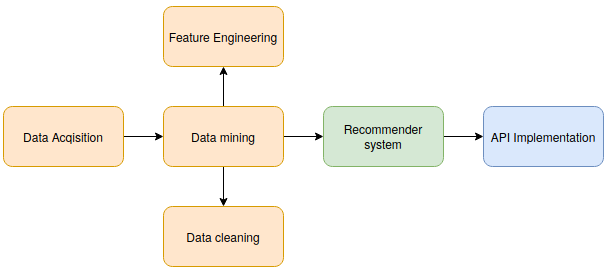
\includegraphics[width=12cm]{contenido/imagenes/initial.png}
    \caption{Metodología de trabajo abreviada. Proceso de tratado de la información para la creación del sistema de recomendación.}
    \label{fig:process}
\end{figure}

El proceso que se seguirá para la creación del sistema de recomendación se muestra en la \autoref{fig:process} y consistirá de los siguientes pasos:
\begin{enumerate}
    \item Adquisición de los datos y limpieza de los mismos.
    %\item Análisis preliminar avanzado de los datos.
    \item Creación del sistema de recomendación.
    \item Creación de la API e integración en el bot de Telegram.
\end{enumerate}
%%%                  %%%
% Document structure   %
%%%                  %%%
\section{Estructura de la memoria}\label{sec:estructura}

El trabajo, como se ha descrito en los capítulos anteriores, tiene como objetivo la creación de un sistema de recomendación de películas, aunque se tratará de incluir en el mismo el flujo \textit{end to end} de tratamiento de la información. El trabajo se estructurará en diferentes capítulos, conteniendo cada uno de ellos una de las partes del flujo. Los capítulos que se incluirán en este trabajo serán los siguientes:

\begin{itemize}
    \item \autoref{chap:recom}: Sistemas de recomendación. Se realizará una explicación de la teoría que existe tras estos sistemas y los diferentes tipos que existen. Se creará el sistema de recomendación.
    \item \autoref{chap:adq}: Estructura de los datos a utilizar y preprocesado de los mismos. En este capítulo se realizará una presentación y explicación de los datos de los que se dispone, de forma que se entiendan los siguientes pasos seguidos.
    %\item \textit{Preliminary Data Analysis}. Caso de uso de análisis de datos para resolución de preguntas de negocio. %Al trabajar con un conjunto de datos siempre es importante realizar un análisis previo, de forma que pueda %entenderse la estructura de los mismos. También se verá la utilidad de disponer de un conjunto de datos %relativamente grande a la hora de responder a preguntas que pueden surgir en relación con la informacion contenida %en los mismos.
    
    \item \autoref{chap:api}: Integración del sistema en una API y creación de un chatbot. Es importante que nuestro sistema de recomendación sea explotable por los usuarios, de nada sirve tener un buen sistema de recomendación si no puede ser usado. Se explicará la creación de un bot de Telegram y cómo crear una API que pueda ser llamada por el bot.
    \item \autoref{chap:resultados}: Resultados. En este capítulo se detallará la metodología seguida para realizar una evaluación del sistema construido en el trabajo y se mostrarán los resultados obtenidos.
    \item \autoref{chap:futuro}: Conclusiones y trabajo futuro. Finalmente, se realizará un repaso de lo desarrollado en el trabajo y se propondrán puntos en los que mejorar el sistema que no hayan podido implementarse por algún motivo.
\end{itemize}

\section{Alcance del trabajo desarrollado}\label{sec:trabajodesarrollado}

En esta memoria, se trata de solventar el problema que se ha comentado en las secciones anteriores. Las plataformas de contenido disponen de sistemas de recomendación potentes, pero con una limitación de origen: solo recomiendan contenido de sus plataformas. Esto hace que si vemos una película concreta en una plataforma y esta nos recomienda otra, es posible que haya mejores recomendaciones que la plataforma en cuestión no esté realizando debido a que no dispone de ese contenido.\\ 

Tal y como se verá en el \autoref{chap:recom}, un tipo de motores de recomendación son los motores basados en contenido. Estos motores se basan en características intrínsecas de las películas y no tanto en las opiniones atómicas de los usuarios. En la solución propuesta en este trabajo, las palabras clave que describen una película son la parte central de la recomendación. Esta elección se ha realizado principalmente por los datos disponibles, ya que los temas de una película, su año de producción o la opinión media de los usuarios son datos relativamente abiertos, mientras que las opiniones concretas de cada usuario son algo propiedad de las plataformas en las que se realizan estas valoraciones, por lo que no tenemos acceso a estos datos.\\ 

Para realizar la recomendación y una vez se ha limpiado el dataset, las películas se distribuyen en un espacio vectorial de keywords y se seleccionan en base a una distancia las más próximas a la película dada. Una vez se tienen las películas más cercanas a la película dada, se establece una heurística que puntúa cada una de estas películas en función de su puntuación, su año de producción y el ratio entre votos e ingresos. Esta heurística trata de, una vez se han seleccionado las películas candidatas a ser recomendadas, tratar de escoger de entre ellas las que probablemente prefiera el usuario. Por ejemplo, creemos que si tras ver una película de Harry Potter se nos recomienda una de magia similar pero del año 1950 es probable que el usuario sea reacio a escogerla.\\

Una de las principales ventajas de nuestro motor de recomendación, es la forma en la que se ha implementado. Al ser un motor agnóstico en términos de plataforma (ya que simplemente tiene datos de las películas y su puntuación en IMDB), necesitábamos un sitio desde el que pudiera ser explotado. De entre todos los posibles, hemos elegido implementarlo en un bot de Telegram, ya que Telegram es una plataforma con una gran expansión y además multiplataforma. Consideramos que la mayoría de usuarios tendrán a mano un dispositivo móvil cuando estén viendo películas, por lo que en cualquier momento pueden escribir un título al bot y éste les enviará las recomendaciones obtenidas.\\

Además, nuestro motor (y en general los motores basados en contenido) tiene una ventaja principal, y es que puede ser actualizado fácilmente con la llegada de nuevas películas a la cartelera. Dado que la información principal que utilizamos son las palabras clave, no necesitamos que un gran número de usuarios haya visto la película en cuestión para que tengamos la información suficiente para recomendar esa nueva película. Esto hace que sea un modelo especialmente beneficioso para que los usuarios puedan descubrir películas menos conocidas que puedan ser de su agrado.\\

Uno de los problemas que suelen tener los motores de recomendación basados en contenido es que en muchas ocasiones recomiendan elementos demasiado similares. Esto se entiende mejor con un ejemplo: imaginemos que nuestra última compra en Amazon es un teclado de ordenador. Si Amazon nos recomendase los productos más parecidos, probablemente nos recomendase otros teclados. Normalmente, cuando hemos comprado un teclado lo último que necesitamos es otro. Las recomendaciones serían, en este caso, tan similares que no serían de utilidad. Sin embargo, consideramos que como nuestro sistema sirve para recomendar películas, este problema se ve mitigado por el mero hecho de que no hay películas tan similares entre sí como productos en Amazon, por ejemplo.


    

        
\chapter{Objetivos y Metodología}\label{chap:objetivos}

Este trabajo tiene como objetivo presentar un caso de uso de las herramientas estudiadas en el máster. Como se ha descrito en capítulos anteriores, el caso de uso elegido es partir de fuentes de datos relacionadas con películas y desarrollar un \textbf{sistema de recomendación} que sea capaz de dar al usuario películas similares a las dadas por él.\\

Para ello se realizará un \textbf{análisis de los datos} y una presentación teórica de los diferentes modelos que existen para crear un sistema de recomendación. Finalmente, se escogerá una técnica concreta en función de sus ventajas y los datos disponibles y se implementará. Para que pueda ser usado en un entorno más productivo y fuera de un ordenador particular, se integrará en el flujo un chatbot que pueda recibir la información del usuario, procesarla, y darle recomendaciones haciendo llamadas a una \textbf{API} que será creada.



%--- Genereal Objectives ---%
\section{Objetivos Generales}\label{sec:objgenerales}

Crear un sistema de recomendación de películas agnóstico a la plataforma en la que el contenido está disponible y utilizable en cualquier entorno. Con este fin, se usarán los datos disponibles en \cite{kaggle}\\

En el mundo actual los usuarios disponen de una gran cantidad de recursos a consumir cuando entran a una plataforma como YouTube o Netflix. Por tanto, se hace necesario que las plataformas sean capaces de entender sus \textbf{gustos y preferencias} para que el cliente consuma la mayor cantidad de contenido posible. En este trabajo se explora la vía de creación de un sistema de recomendación basado en contenido que, a partir de modelos de lenguaje sea capaz de entender el contenido de cada una de las películas y a partir de una preferencia dada por el usuario, le pueda recomendar otras películas similares para ver. Además, destruirá la barrera de la plataforma que imponen los sistemas embebidos dentro de estas. El sistema desarrollado recomendará sin tener en cuenta dónde está disponible el contenido, con el fin de ampliar los horizontes del usuario.\\

Como se verá más adelante, en el \autoref{chap:recom}, existen diferentes tipos de sistemas de recomendación. En este trabajo nos centraremos en sistemas basados en contenido, dado que tienen ventajas como su capacidad para recomendar productos nuevos y la no necesidad de información del usuario. Además, la información sobre las películas es más sencilla de obtener en la red.\\

Explicado esto, este trabajo se engloba dentro de los trabajos de Tipo 2 (desarrollo de software). Se realizará un desarrollo de una solución \textit{end to end} al problema de la recomendación de contenidos a usuarios. Desde la recopilación de datos y metadatos sobre películas, hasta la creación de la interfaz a través de la que el usuario final podrá hacer solicitudes al sistema creado y obtener recomendaciones.\\

Además, se realizará una revisión de los diferentes sistemas de recomendación existentes en la actualidad y su aparición en los últimos años.\\

%Finalmente, creemos necesario realizar un análisis de los datos que se utilizaran, previo a la creación del sistema de recomendación. En el %campo de la Ciencia de Datos se considera una buena práctica la realización de un análisis de los datos de forma previa a la creación del %sistema de recomendación en sí. Además de este análisis preliminar, mostraremos cómo el disponer de un conjunto lo suficientemente extenso de %datos puede servir para responder preguntas sobre los usuarios, que pueden ayudar al desarrollo del negocio.\\


%--- Specific Objectives ---%
\section{Objetivos Específicos}\label{sec:objespecificos}

Una vez descritos los objetivos generales del trabajo que se desarrollará, se hace necesario desgranarlos en una serie de objetivos más específicos que puedan ser más fácilmente analizados y desarrollados y para los que pueda establecerse un grado de consecución.

\begin{itemize}
    \item Conocer las fuentes de datos disponibles, el formato de los datos de películas y actores y sus posibilidades de explotación.
    \item Describir los datos disponibles y analizar los datos para sacar conclusiones sobre los mismos.
    %\item \textbf{IDENTIFICAR} tendencias a partir de los datos y \textbf{RESPONDER} a partir de ellos a preguntas que puedan surgir.
    \item Desarrollar el sistema de recomendación de películas que permita a los usuarios obtener recomendaciones a partir de una película dada..
    \item Integrar la solución desarrollada en un entorno API-bot que pueda ser usada por usuarios finales.
    \item Verificar la usabilidad de la solución y evaluar el rendimiento de la misma.
    \item Identificar las flaquezas del sistema y los puntos de mejora para proponer próximos pasos.
\end{itemize}

%--- Work Methodology ---%
\section{Metodología de Trabajo}\label{sec:metodología}

En este trabajo, se ha utilizado una metodología definida de forma inicial, aunque posteriormente se han tenido que ir realizando adaptaciones de la misma a medida que se desarrollaba el mismo.\\

En primer lugar, hay se definió de forma concreta el problema que se quería resolver y se realizó una investigación bibliográfica con la finalidad de conocer los diferentes sistemas de recomendación que existen, de forma que pudiéramos definir correctamente el tipo de sistema que se quería utilizar y los datos necesarios.\\

Partiendo del problema descrito en la introducción, se buscó un conjunto de datos que hiciera posible dar una solución al problema. El conjunto de datos disponible está disponible en \cite{kaggle}.\\

Una vez encontrados unos datos con los que trabajar, se definieron los pasos a seguir para la implementación del proyecto y la resolución del problema:
\begin{enumerate}
    \item Limpieza de los datos: En un proyecto de análisis de datos real, es una fase imprescindible. En esta fase se revisan los datos originales, se borran los datos incorrectos y se tratan los valores incorrectos o faltantes. Las herramientas a utilizar en esta etapa serán principalmente Python y la librería Pandas.
    \item Preprocesamiento de los datos: Una vez se hayan limpiado los datos, será necesario realizar un preprocesamiento de los mismos para que sirvan de entrada al sistema de recomendación, fase en la que se usará Python y librerías de procesamiento de lenguaje natural si fuera necesario.
    \item Construcción del sistema de recomendación: Tras la investigación bibliográfica y el preprocesamiento de los datos, se construirá el sistema de recomendación en sí. El objetivo es poder dar 3 recomendaciones de películas dada una de entrada, que pueda tener faltas de ortografía, de forma que el sistema sea más flexible.
    \item Integración del sistema en una API: Desde el principio, la intención ha sido crear un sistema usable y desde una perspectiva \textit{end to end}. En muchas ocasiones este tipo de trabajos se quedan en una mera investigación bibliográfica y teórica. Sin embargo, la intención es que el sistema sea realmente usable por todo el mundo que lo desee. En esta fase se valorarán las diferentes alternativas para proveer de una interfaz al sistema creado, generando un servicio web desde el que puedan realizarse recomendaciones.
\end{enumerate}
        \chapter{Adquisición y limpieza de los datos}\label{chap:adq}

En cualquier proyecto de Data Science es necesario trabajar con una cantidad relativamente grande de datos. Sin embargo, normalmente el estado y el formato en el que se encuentran los datos de los que puede disponerse en Internet no se adecúan a las necesidades concretas del proyecto. Además, es habitual encontrar fuentes de datos con un número elevado de campos; es también tarea de esta etapa obtener los campos necesarios para el proyecto con el fin de aligerar las ejecuciones, ya que la mayoría de modelos son sensibles a la cantidad de campos. Por tanto, el proceso de adquisición y limpieza de los datos se convierte en una parte muy importante del proceso. Los objetivos principales de la etapa de limpieza de los datos son los siguientes:
\begin{itemize}
    \item Adaptar el formato a los requerimientos del proyecto.
    \item Eliminar registros incorrectos.
    \item Completar registros en los que falte alguno de los datos.
    \item Dejar únicamente los campos necesarios para el proyecto a desarrollar.
\end{itemize}

Para la creación del sistema de recomendación de películas basado en contenido que se desarrollará en este proyecto se utilizará un dataset consistente en información sobre varios miles de películas disponible en \url{https://tinyurl.com/ypfdw8w}. El dataset consiste en dos ficheros: películas y créditos. Los campos disponibles en los ficheros son los siguientes:

\begin{itemize}
    \item Películas
    \begin{itemize}
        \item budget: Presupuesto de la película en Dólares.
        \item genres: Generos cinematográficos asociados a la película.
        \item homepage: Página web de la productora de la película.
        \item id: Identificador único dentro del dataset.
        \item plot\_keywords: Palabras clave.
        \item original\_language: Idioma original
        \item original\_title: Título original de la película
        \item overview: Resumen
        \item popularity: Popularidad (unidades desconocidas)
        \item production\_companies: Compañías encargadas de la producción
        \item production\_countries: Paises productores de la película
        \item release\_date: Fecha de lanzamiento de la película
        \item revenue: Recaudación de la película en dólares
        \item runtime: Días en cartelera
        \item spoken\_languages: Idiomas hablados en la película
        \item status: Estado de la película
        \item tagline: Subtítulo
        \item title: Título en inglés
        \item vote\_average: Promedio de votos en IMDB
        \item vote\_count: Número de votos en IMDB
    \end{itemize}
    \item Créditos
    \begin{itemize}
        \item movie\_id: Identificador de la película (para unirlo con el dataset anterior).
        \item title: Título en inglés de la película
        \item cast: Actores que aparecen (en orden e importancia). Campo en formato JSON.
        \item crew: Equipo participante en la película, es un JSON con una lista de diccionarios. Cada elemento de la lista tiene el nombre del participante y el cargo.
    \end{itemize}
\end{itemize}

En la \autoref{tab:peliculas} puede verse un análisis descriptivo de los campos numéricos de los datos anteriormente mencionados. El resto de campos son campos de texto:

\begin{table}[h]
\centering
\resizebox{0.8\textwidth}{!}{%
\begin{tabular}{lrrrrrrr}
\toprule
{} &        budget &   popularity &       revenue &      runtime &  vote\_average &    vote\_count \\
\midrule
count &  $4.8\cdot 10^{3}$ &  $4803.0$ &  $4.8\cdot 10^{3}$ &  $4801.0$ &   $4803.0$ &   $4803.0$ \\
mean  &  $2.9\cdot 10^{7}$ &   $21.5$ &  $8.2\cdot 10^{7}$ &   $106.9$ &      $6.1$ &    $690.2$ \\
std   &  $4.1\cdot 10^{7}$ &   $31.8$ &  $1.6\cdot 10^{8}$ &    $22.6$ &      $1.2$ &   $1234.5$ \\
min   &  $0.0\cdot 10^{0}$ &       $0.0$ &  $0.0\cdot 10^{0}$ &     $0.0$ &      $0.0$ &      $0.0$ \\
25\%   &  $7.9\cdot 10^{5}$ &    $4.7$ &  $0.0\cdot 10^{0}$ &    $94.0$ &      $5.6$ &     $54.0$ \\
50\%   &  $1.5\cdot 10^{7}$ &   $12.9$ &  $1.9\cdot 10^{7}$ &   $103.0$ &      $6.2$ &    $235.0$ \\
75\%   &  $4.0\cdot 10^{7}$ &   $28.3$ &  $9.3\cdot 10^{7}$ &   $118.0$ &      $6.8$ &    $737.0$ \\
max   &  $3.8\cdot 10^{8}$ &  $875.6$ &  $2.8\cdot 10^{9}$ &   $338.0$ &     $10.0$ &  $13752.0$ \\
\bottomrule
\end{tabular}}
\caption{Análisis descriptivo de las variables numéricas de los datos de entrada. Se muestra para cada campo el número de filas informadas, la media, la desviación estándar y los cuartiles.}
\label{tab:peliculas}
\end{table}

\newpage
\section{Importación de datos de películas}

El primer paso en la etapa de adquisición de los datos consiste en leer ambos ficheros (en formato csv) y obtener los DataFrame de Pandas correspondientes. Las columnas genres, keywords, production\_countries, production\_companies, spoken\_languages, cast y crew están en formato json en origen. Es por ello que en las funciones de lectura de los datos tienen un trato especial. Las funciones implementadas son las siguientes:

\begin{lstlisting}[language=Python, caption={Lectura de los datos del fichero de películas. Se carga el fichero desde la ruta y se mapea la fecha de lanzamiento a un objeto de tipo fecha.}]
import json
import pandas as pd
def carga_peliculas(ruta):
    """Función utilizada para cargar el dataset de las películas. Se transforma a fecha el campo de fecha de salida
    y se cargan como listas los campos que están guardados como json.
    Args:
        ruta (str): Ruta hasta el archivo de tmdb_5000_peliculas.csv
    Returns:
        pd.DataFrame: Dataframe de pandas con la información del csv
    """
    df = pd.read_csv(ruta)
    df['release_date'] = pd.to_datetime(df['release_date']).apply(lambda x: x.date())
    json_columns = ['genres', 'keywords', 'production_countries', 'production_companies', 'spoken_languages']
    for columna in json_columns:
        df[columna] = df[columna].apply(json.loads)
    return df
\end{lstlisting}

\begin{lstlisting}[language=Python, caption={Lectura de los datos del fichero de créditos. Se carga el fichero desde la ruta dada.}]
def carga_creditos(ruta):
    """Función utilizada para cargar el dataset de los créditos. Se cargan como listas los campos que están guardado
    Args:
        ruta (str): Ruta hasta el archivo de tmdb_5000_creditos.csv
    Returns:
        pd.DataFrame:
    """
    df = pd.read_csv(ruta)
    json_columns = ['cast', 'crew']
    for columna in json_columns:
        df[columna] = df[columna].apply(json.loads)
    return df
\end{lstlisting}

Pandas es una librería rápida, flexible, opensource y relativamente fácil de usar. Está implementada en Python y es una de las librerías más usadas para realizar tareas de análisis y manipulación de datos. En este proyecto esta librería será utilizada de forma extensiva. Con estas dos funciones se consigue tener los datos en el tipo de dato que proporciona Pandas, el DataFrame. Este tipo de objeto tiene formato tabular (donde una fila es un registro y una columna un atributo del registro) y tiene multitud de métodos implementados para la transformación de datos.\\

En esta primera etapa de importación, el objetivo es obtener un único DataFrame que contenga información de ambos conjuntos de datos. Un problema habitual que tiene lugar al juntar dos ficheros es la información faltante de los ficheros. Hay que tratar de forma especial el acceso a los datos de cada DataFrame a la hora de juntarlos, pues puede que haya campos que no estén informados. Para ello, definimos una función que accede de forma segura a los datos, ya que en caso de no encontrarlo devuelve nulo, evitando errores de ejecución.

\begin{lstlisting}[language=Python, caption={Acceso a los datos de forma segura. Se utiliza como proxy para no acceder directamente al valor. De esta forma, si se da un error, en vez de tener un error de ejecución se devuelve nulo.}]
def get_elemento(contenedor, valores_indice):
    """Función para acceder de forma segura a valores. En caso de que no se encuentre uno de ellos, se devuelve NaN
    en vez de lanzar un error.
    Args:
        contenedor (list): Lista/ contenedor de la que quieren extraerse los valores
        valores_indice (list): Lista de índices a extraer del contenedor
    Returns:
        any: Valores extraidos
    """
    result = contenedor
    try:
        for idc in valores_indice:
            result = result[idc]
        return result
    except IndexError or KeyError:
        return pd.np.nan
\end{lstlisting}

Uno de los campos a extraer del fichero de créditos es el de director. Este campo se encuentra dentro del campo de crew (en formato json) con la clave director. Por tanto, para añadirlo al DataFrame es necesario buscarlo. Para ello se define la función get\_director.
\begin{lstlisting}[language=Python, caption= {Obtención de una lista de directores extraídos del campo crew. Se itera por todos los miembros del equipo y se retienen únicamente aquellos que tienen el cargo de director.}]
def get_director(datos_equipo):
    """Devuelve el director dado un json con toda la composición del equipo de la película.
    Args:
        datos_equipo (json): JSON con el equipo que ha realizado la película
    Returns:
        str: Director de la película
    """
    directores = [x['name'] for x in datos_equipo if x['job'] == 'Director']
    return get_elemento(directores, [0])
\end{lstlisting}

Como se ha visto anteriormente, el objetivo del proyecto es crear un sistema de recomendación de películas basado en contenido. Por tanto, resulta vital conseguir información del contenido de las películas. El campo fundamental para conseguir este fin es el campo keywords, que contiene las palabras clave de cada película. Este campo está en origen en formato JSON, con información que no es relevante para el objetivo del proyecto. Para obtener únicamente las palabras clave se implementa pipe\_flatten\_names que extrae estas palabras clave.
\begin{lstlisting}[language=Python, caption= {Extracción de las palabras clave a partir del JSON del DataFrame. }]
def aplana_nombres(keywords):
    """Obtiene una lista con las keywords separadas por un pipe | extrayéndolas del json.
    Args:
        keywords (json): keywords de la película
    Returns:
        str: keywords de la película juntas
    """
    return '|'.join([x['name'] for x in keywords])
\end{lstlisting}

Para terminar con la etapa de importación y carga de los datos, se crea la función que añade al DataFrame de películas la información de credits necesaria.
\begin{lstlisting}[language=Python, caption= {El conjunto de datos se encuentra en dos ficheros separados y con estructuras diferentes. Se juntan esas dos colecciones un un único conjunto de datos.}]
def combina_colecciones(peliculas, creditos):
    """Aplica una serie de funciones para añadir información al dataset de películas a partir del
    conjunto de datos de créditos
    Args:
        peliculas (pd.DataFrame): DataFrame obtenido de leer el archivo de películas
        creditos (pd.DataFrame): DataFrame obtenido de leet el archivo de créditos
    Returns:
        pd.DataFrame: DataFrame con la información conjunta
    """
    tmdb_peliculas = peliculas.copy()
    tmdb_peliculas.rename(columns=EQUIVALENCIAS_TMDB_IMDB, inplace=True)
    tmdb_peliculas['title_year'] = pd.to_datetime(tmdb_peliculas['release_date']).apply(lambda x: x.year)
    # I'm assuming that the first production country is equivalent, but have not been able to validate this
    tmdb_peliculas['country'] = tmdb_peliculas['production_countries'].apply(lambda x: get_elemento(x, [0, 'name']))
    tmdb_peliculas['language'] = tmdb_peliculas['spoken_languages'].apply(lambda x: get_elemento(x, [0, 'name']))
    tmdb_peliculas['director_name'] = creditos['crew'].apply(get_director)
    tmdb_peliculas['actor_1_name'] = creditos['cast'].apply(lambda x: get_elemento(x, [1, 'name']))
    tmdb_peliculas['actor_2_name'] = creditos['cast'].apply(lambda x: get_elemento(x, [2, 'name']))
    tmdb_peliculas['actor_3_name'] = creditos['cast'].apply(lambda x: get_elemento(x, [3, 'name']))
    tmdb_peliculas['genres'] = tmdb_peliculas['genres'].apply(aplana_nombres)
    tmdb_peliculas['plot_keywords'] = tmdb_peliculas['plot_keywords'].apply(aplana_nombres)
    return tmdb_peliculas
\end{lstlisting}

Por último, se cargan las librerías necesarias para el proyecto y se leen los datos de los ficheros, usando las funciones definidas anteriormente.
\begin{lstlisting}[language=Python, caption=Código usado para la carga de los datos. Se aplican las funciones definidas anteriormente para obtener, a partir de los CSV un único dataframe, que será con el que se trabaje el resto del tiempo]
import numpy as np
import matplotlib as mpl
import matplotlib.pyplot as plt
import seaborn as sns
import math, nltk, warnings
from nltk.corpus import wordnet
from sklearn import linear_model
from sklearn.neighbors import NearestNeighbors
from fuzzywuzzy import fuzz
from wordcloud import WordCloud, STOPWORDS
plt.rcParams["patch.force_edgecolor"] = True
plt.style.use('fivethirtyeight')
mpl.rc('patch', edgecolor = 'dimgray', linewidth=1)
from IPython.core.interactiveshell import InteractiveShell
InteractiveShell.ast_node_interactivity = "last_expr"
pd.options.display.max_columns = 50
%matplotlib inline
warnings.filterwarnings('ignore')

#Definimos la función a utilizar para obtener el lexema de las palabras.
PS = nltk.stem.PorterStemmer()
#__________________
# load the dataset
#df_inicial = pd.read_csv("../input/movie_metadata.csv")
creditos = carga_creditos("../RecommendationEngine/datos/tmdb_5000_credits.csv")
peliculas = carga_peliculas("../RecommendationEngine/datos/tmdb_5000_movies.csv")
df_inicial = combina_colecciones(peliculas, creditos)
\end{lstlisting}

Con esto, se consigue tener un único DataFrame sobre el que trabajar.

\newpage
\section{Limpieza y transformación de los datos}

Una vez se han importado y cargado los datos, la siguiente etapa es el limpiado de los datos, tanto para lidiar con los posibles datos faltantes.

\subsection{Entradas duplicadas}

En ocasiones los datasets que se encuentran en Internet no están en un estado perfecto, y en ocasiones se tienen datos duplicados. Es importante comprobar si existen datos duplicados, ya que si no a la hora de crear modelos puede darse más importancia a unos registros que a otros, lo cual resulta un error de concepto. En primer lugar, por tanto, comprobamos la existencia de entradas duplicadas.
\begin{lstlisting}[language=Python, caption=Entradas duplicadas. Se buscan entradas duplicadas a partir del id de la película y se devuelve la cantidad de películas repetidas.]
entradas_duplicadas = df_inicial[df_inicial.id.duplicated()]
entradas_duplicadas.shape
\end{lstlisting}
El resultado es que no existen entradas duplicadas. Sin embargo, comprobar la duplicidad de esta forma tan genérica puede no solucionar todos los posibles problemas. Por ejemplo, podría haber una entrada con un error ortográfico o con diferencias mínimas. En este caso, cada entrada se corresponde con una película, por lo que tener dos entradas que únicamente difieren en, por ejemplo, el presupuesto, podría considerarse una entrada duplicada. Dado que son datos de películas, buscaremos entradas con el mismo título. 

\begin{lstlisting}[language=Python, caption=Entradas con título duplicado. Se buscan películas que tengan el mismo título, para realizar un análisis y determinar si se trata de entradas duplicadas que hay que filtrar o no.]
df_temp = df_inicial
lista_var_de_duplicados = ['movie_title', 'title_year', 'director_name']
lista_duplicados = df_temp['movie_title'].map(df_temp['movie_title'].value_counts() > 1)
df_temp[lista_duplicados][lista_var_de_duplicados].sort_values('movie_title')
\end{lstlisting}

El resultado se muestra en la \autoref{tab:duplicated_entries}. Como puede comprobarse, únicamente hay tres parejas de películas con el mismo título. Analizándolo a simple vista puede verse que se trata de remakes, por lo que no podemos considerarlo como entradas duplicadas, ya que pueden diferir en calidad e incluso en alguna palabra clave.\\

\begin{table}[h]
\centering
\begin{tabular}{llrl}
\toprule
\textbf{id} &     \textbf{movie\_title} &  \textbf{title\_year} &        \textbf{director\_name} \\
\midrule
1359 &           Batman &      1989 &           Tim Burton \\
4267 &           Batman &      1966 &  Leslie H. Martinson \\
3647 &  Out of the Blue &      1980 &        Dennis Hopper \\
3693 &  Out of the Blue &      2006 &       Robert Sarkies \\
972  &         The Host &      2013 &        Andrew Niccol \\
2877 &         The Host &      2006 &         Bong Joon-ho \\
\bottomrule
\end{tabular}
\caption{Entradas con el título duplicado. Puede verse que se no se trata de una errata, ya que aunque las películas se llaman igual, son de años diferentes y tienen directores diferentes. Esto significa que, probablemente, se trate de \textit{remakes} de las películas originales.}
\label{tab:duplicated_entries}
\end{table}

Por tanto, puede concluirse que en el dataset no existen entradas duplicadas. A pesar de tener el mismo dataset al inicio de este apartado que ahora, se ha incluido por completitud, ya que es un paso que debe realizarse siempre.

\subsection{Limpieza de las keywords de las películas}

Las keywords tendrán un papel fundamental en el funcionamiento del sistema. De hecho, como se verá en el \autoref{chap:creacion}, las recomendaciones se realizarán en base a la similaridad entre películas, y para esta medida se usarán las keywords. Por tanto, se hace necesario analizar el contenido de esta variable, puesto que se realizará un uso extensivo de ella.\\

Inicialmente, el dataset contiene un total de 9474 keywords. En la \autoref{fig:keywords_histogram} se muestra la distribución del número de keywords. Puede verse que aun habiendo casi el doble de keywords que de películas, la mayoría de películas contienen entre 5 y 15 keywords, por lo que el número de keywords no es preocupante.
\begin{figure}[H]
    \centering
    \captionsetup{width=10cm}
    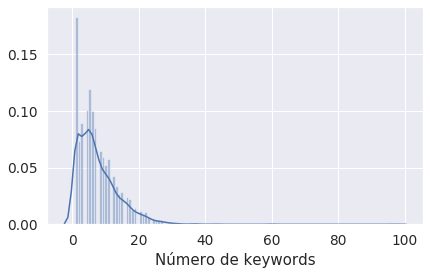
\includegraphics[width=12cm]{contenido/imagenes/keyword_histogram.png}
    \caption{Histograma con el número de keywords de cada película.}
    \label{fig:keywords_histogram}
\end{figure}

Sin embargo, tratar con lenguaje natural siempre implica poner especial atención en lo que se consideran palabras diferentes. Es lógico pensar que a la hora de poner las keywords de las películas no se ha tenido en cuenta las posibles similitudes entre keywords ni se han asignado de una lista cerrada.\\

Los seres humanos nos expresamos de forma muy diferente y probablemente las keywords hayan sido asignadas por personas diferentes. Por lo cual es esperable que haya keywords que signifiquen aproximadamente lo mismo pero que por tener distintas grafías actualmente se considerarían diferentes palabras.\\

El lenguaje de Python es ampliamente utilizado en la disciplina de la ciencia de datos, es por ello que existen numerosas librerías de inestimable ayuda para el NLP. Una de las más conocidas es NLTK \cite{NLTK} (\textbf{N}atural \textbf{L}anguage \textbf{T}ool\textbf{K}it).\\

En este proyecto es importante extraer el significado original de las keywords, es decir, no importa si la keyword es ``drama'' o ``dramático'', ya que significan lo mismo. En este caso utilizamos la librería NLTK, que en concreto implementa una función denominada \texttt{PorterStemmer}\cite{porter}, que es una función que sirve para extraer lexemas de las palabras. Con este paso se consigue extraer la raíz de la palabra para evitar problemas con plurales, etc. En primer lugar se implementa la función\texttt{keywords\_inventory} que recoge las keywords y crea un diccionario para ver en qué palabra queda otra.

\begin{lstlisting}[language=Python, caption= Obtención del lexema de cada keywords y creación del diccionario de equivalencia. Se itera sobre cada una de las películas y se extraen sus palabras clave. Para evitar palabras derivadas con el mismo significado, se extrae y se almacena el lexema de cada keyword.]
def inventario_keywords(dataframe, columna = 'plot_keywords'):
    """Devuelve un diccionario con las palabras que derivan de cada lexema
    a partir de un DataFrame y la columna de la que se quiere extraer
    Args:
        dataframe (pd.DataFrame): DataFrame del que obtener la información.
        columna (str, optional): Nombre de la columna. Por defecto 'plot_keywords'.
    Returns:
        list: Keywords finales que aparecen
        dict: Relación lexema <-> palabras
        dict: Palabra más corta derivada del lexema
    """
    PS = nltk.stem.PorterStemmer()
    keywords_raices  = dict()  # recoger las palabras de cada lexema
    keywords_selecciona = dict()  # asociacion: lexema <-> keyword
    category_keys = []
    icuenta = 0
    for s in dataframe[columna]:
        if pd.isnull(s): continue
        for t in s.split('|'):
            t = t.lower()
            raiz = PS.stem(t)
            # Para cada lexema, un set con las palabras que lo usan
            if raiz in keywords_raices:                
                keywords_raices[raiz].add(t)
            else:
                keywords_raices[raiz] = {t}
    
    for s in keywords_raices.keys():
        if len(keywords_raices[s]) > 1:  
            longtud_min = 1000
            for k in keywords_raices[s]:
                if len(k) < longtud_min:
                    clave = k ; longtud_min = len(k)            
            category_keys.append(clave)
            keywords_selecciona[s] = clave
        else:
            category_keys.append(list(keywords_raices[s])[0])
            keywords_selecciona[s] = list(keywords_raices[s])[0]
                   
    print("Número de keywords en la variable: '{}': {}".format(columna,len(category_keys)))
    return category_keys, keywords_raices, keywords_selecciona
\end{lstlisting}

Con el fin de limpiar el dataset se implementa la función \texttt{df\_keywords\_replacement}. Algunos cambios que realiza este paso es tomar por iguales orc y orcs, spy y spying o time travel y time traveler.
\begin{lstlisting}[language=Python, caption= Extracción del lexema de las keywords. Reemplaza las apariciones de una palabra clave por su lexema, con el fin de extraer el significado de la palabra clave y reducir su cantidad.]
def df_reemplazo_keywords(df, dicc_reemplazo, raiz = False, columna = 'plot_keywords'):
    """Reemplaza las palabras clave de una película por las formas básicas de las mismas.
    Args:
        df (pd.DataFrame): DataFrame que contiene la información de las películas
        dicc_reemplazo (dict): Diccionario con los cambios
        raiz (bool, optional): Controla si se obtienen las raices de las palabras de las
        keywords. Por defecto False.
        columna (str, optional): Columna en la que realizar la transformación. Por defecto 'plot_keywords'.
    Returns:
        pd.DataFrame: DataFrame con las sustituciones realizadas
    """
    PS = nltk.stem.PorterStemmer()
    df_nuevo = df.copy(deep = True)
    for indice, fila in df_nuevo.iterrows():
        cadena = fila[columna]
        if pd.isnull(cadena): continue
        nueva_lista = []
        for s in cadena.split('|'): 
            clave = PS.stem(s) if raiz else s
            if clave in dicc_reemplazo.keys():
                nueva_lista.append(dicc_reemplazo[clave])
            else:
                nueva_lista.append(s)       
        df_nuevo.at[indice, columna] = '|'.join(nueva_lista)
    return df_nuevo
\end{lstlisting}

Finalmente, se realiza el cambio en el dataset de la siguiente manera:

\begin{lstlisting}[language=Python, caption= Sustitucion de las keywords por su forma primitiva.]
keywords, keywords_roots, keywords_select = keywords_inventory(df_duplicate_cleaned,
                                                               column = 'plot_keywords')
df_keywords_cleaned = df_keywords_replacement(df_duplicate_cleaned, keywords_select,
                                               roots = True)
\end{lstlisting}

\subsection{Sinónimos}

En la sección anterior de la memoria, se han explicado las peculiaridades de trabajar con un dataset que contenga texto, así como la estrategia seguida par reducir la cantidad de keywords. Sin embargo, únicamente hemos agrupado las keywords por su lexema, que es además la forma más simple de realizar esta agrupación. Por ejemplo, si hubiera dos películas, una con la keyword alien y otra con la keyword extraterrestre, únicamente con el paso anterior seguirían siendo películas diferentes.\\

En esta sección se va un paso más allá. La librería NLTK además de extractores de lexema, incluye un submódulo de corpus. En este caso se utilizará el corpus de WordNet. Consiste en una base de datos léxica de sustantivos, verbos, adjetivos y adverbios en inglés agrupados en conjuntos de sinónimos cognitivos, expresando cada uno un concepto diferente. Se trata de una herramienta con muchísimo potencial para el análisis de texto.\\

En este caso concreto, se utilizará el corpus de WordNet \cite{WordNet} implementado en la librería NLTK para sustituir las keywords con menos apariciones por sus sinónimos más frecuentes. Por ejemplo, la keyword extraterrestrial aparece un total de 4 veces. Es posible que sustituirla por alien en esas 4 películas haga que las películas de aliens estén mejor relacionadas, ya que no hay apenas diferencia entre los significados. En concreto, las keywords con menos de 5 apariciones serán sustituidas por su sinónimo más frecuente. Con esto se reemplaza aproximadamente el $6 \%$ de las keywords.
\begin{lstlisting}[language=Python, caption= Sustitución de las palabras menos frecuentes por sus sinónimos. En este caso, puede ser un problema el tener palabras dfierentes con el mismo significado, ya que podría enmascarar relaciones entre películas. Para ello, se buscan los sinónimos de las keywords y se sustituye la keyword por el sinónimo con mayor número de apariciones.]
def prueba_keyword(palabra, keyword_apariciones, umbral):
    """Devuelve si una palabra aparece un número mayor de veces que el umbral señalado
    Args:
        palabra (str): Palabra a buscar
        keyword_apariciones (dict): Diccionario con las apariciones de cada keyword
        umbral (int): Umbral
    Returns:
        bool: True si aparece un número mayor de veces
    """
    return (False , True)[keyword_apariciones.get(palabra, 0) >= umbral] 

veces_keyword.sort(key = lambda x:x[1], reverse = False)
keyword_cuenta = dict()
for s in veces_keyword:
    keyword_cuenta[s[0]] = s[1]
# Creación de un diccionario para reemplazar keywords por sinónimos de mayor frecuencia
palabra_reemplazo = dict()
icuenta = 0
for _, [palabra, num_apariciones] in enumerate(veces_keyword):
    if num_apariciones > 5:
        continue  # Sólo las keywords que aparecen menos de 5 veces
    lexema = toma_sinonimos(palabra)
    if len(lexema) == 0:
        continue     #Caso de plurales
    lista_palabras = [(s, keyword_cuenta[s]) for s in lexema 
                  if prueba_keyword(s, keyword_cuenta, keyword_cuenta[palabra])]
    lista_palabras.sort(key = lambda x:(x[1],x[0]), reverse = True)    
    if len(lista_palabras) <= 1:
        continue       # NO se reemplaza
    if palabra == lista_palabras[0][0]:
        continue    # Reemplazo por sí mismo
    icuenta += 1
    if  icuenta < 8:
        print('{:<12} -> {:<12} (inic: {})'.format(palabra, lista_palabras[0][0], lista_palabras))
    palabra_reemplazo[palabra] = lista_palabras[0][0]
\end{lstlisting}

Conviene recordar que el objetivo de este proyecto es crear un sistema de recomendación de películas \textbf{basado en contenido}. Por ello, de poco sirve tener una keyword que aparezca en una cantidad muy reducida de películas.

\begin{figure}[H]
    \centering
    \captionsetup{width=12cm}
    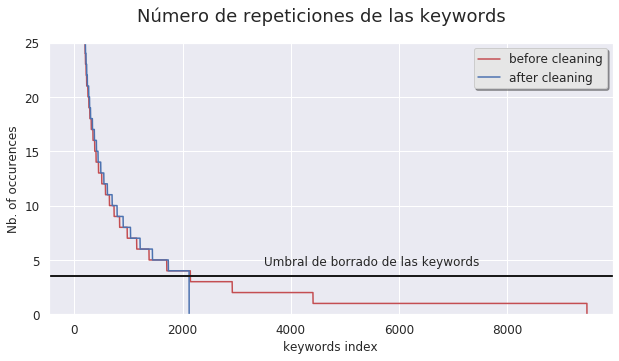
\includegraphics[height=9.3cm]{./contenido/imagenes/keyword_cleaning.png}
\caption{Repeticiones de las keywords antes y después de la limpieza.}
\label{fig:key_cleaning}
\end{figure}

En este caso se ha decidido eliminar las keywords con menos de $3$ repeticiones, que como puede verse en la \autoref{fig:key_cleaning} afecta a la mayoría de keywords, pasando a tener aproximadamente $6500$ keywords menos. Puede parecer que perdemos mucha información, pero lo que se busca es tener relaciones potentes. Además, como se verá más adelante, se definirá una distancia entre películas, por lo que no es conveniente tener demasiadas dimensiones, ya que se podría tener el problema de la dimensionalidad \cite{wiki:CurseOfDimensionality}

\newpage
\section{Imputación de valores faltantes}

En estadística, la imputación es el proceso de reemplazar los datos faltantes con valores sustitutos. Son tres los principales problemas que causan los datos faltantes:
\begin{itemize}
    \item Introducir una cantidad sustancial de bias.
    \item Hacer más complicado el tratamiento de los datos.
    \item Empeorar la eficiencia de los modelos.
\end{itemize}

Siempre es interesante realizar un análisis de las entradas que tienen datos faltantes, ya que por ejemplo si se tuviera un dataset con información de varias estaciones de medición, podría ser que los datos faltantes no fueran aleatorios, sino producidos por una situación concreta de alguna de las estaciones.\\

Existen dos técnicas principales para imputar estos datos:

\begin{itemize}
    \item Sustitución promedio: Implica reemplazar los valores faltantes con la media de esa variable en los demás casos. Tiene el beneficio de no cambiar la media de la distribución. Sin embargo, atenúa las correlaciones que implican a la variable imputada.
    \item Imputación mediante regresión: Es, por así decirlo, la forma opuesta de realizar la imputación. Imputa una de las variables fijándose en una o varias de las demás. En este caso no se genera cambio en la correlación entre variables pero sí se afecta a la media. Otro problema es que supone que la regresión no tiene un término de error asociado y que es, por tanto, una regresión con $R² = 1$.
\end{itemize}

En la \autoref{fig:correlation} se muestra la matriz de correlación entre las variables del dataset, lo cual aporta información sobre qué variables usar para predecir otras.

\begin{figure}[H]
    \centering
    \captionsetup{width=12cm}
    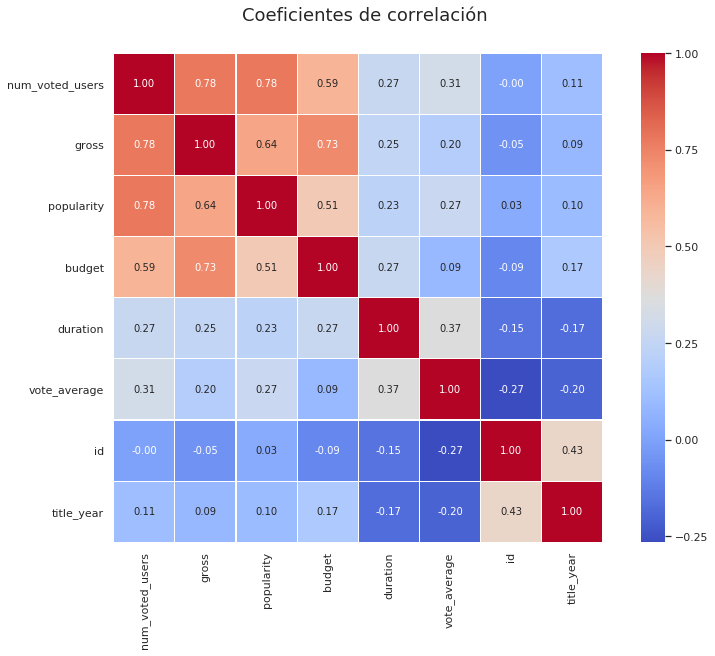
\includegraphics[height=10cm]{./contenido/imagenes/correlation.png}
\caption{Correlación entre las variables del dataset. La matriz es simétrica, ya que la correlación entre A y B es igual que la correlación entre B y A.}
\label{fig:correlation}
\end{figure}

En este caso, se utilizarán varios tipos de imputación, algunos adecuados al dominio concreto del problema. Es necesario resaltar que únicamente se imputarán aquellas variables que sean necesarias para la creación propiamente dicha del recomendados. En la \autoref{fig:completion} se muestran los porcentajes de completitud de cada una de las variables que restan.

\begin{figure}[H]
    \centering
    \captionsetup{width=12cm}
    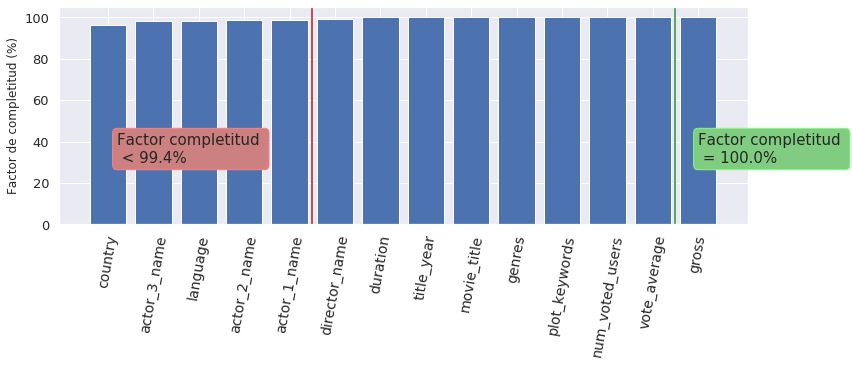
\includegraphics[width= 13cm]{./contenido/imagenes/completion.png}
\caption{Completitud de las variables del dataset. La mayoría de variables tienen un factor de completitud bastante grande.}
\label{fig:completion}
\end{figure}


\subsection{Años faltantes}

En el sistema de recomendación, la variable año se utilizará para recomendar al usuario películas relativamente coetáneas a la dada por el usuario. Con el fin de tener el año informado en la mayor cantidad posible de registros, se completará el año teniendo en cuenta los años de creación del resto de películas de su director y los 3 actores principales, realizando un promedio entre todos ellos. Con este fin se implementa la función \texttt{fill\_year}.

\begin{lstlisting}[language=Python, caption={Completado de la variable año en el dataset utilizando el promedio de los años de las películas de su director y actores principales.}]
def rellena_ano(df):
    """Completa la columna faltante del año teniendo en cuenta la media
    de los periodos de actividad de los actores y el director.
    """
    col = ['director_name', 'actor_1_name', 'actor_2_name', 'actor_3_name']
    ano_habitual = [0 for _ in range(4)]
    var = [0 for _ in range(4)]
    # Año medio de actividad para los actores y el director
    for i in range(len(col)):
        ano_habitual[i] = df.groupby(col[i])['title_year'].mean()
    # Diccionario que recoja esta información
    ano_actor = dict()
    for i in range(4):
        for s in ano_habitual[i].index:
            if s in ano_actor.keys():
                if pd.notnull(ano_habitual[i][s]) and pd.notnull(ano_actor[s]):
                    ano_actor[s] = (ano_actor[s] + ano_habitual[i][s])/2
                elif pd.isnull(ano_actor[s]):
                    ano_actor[s] = ano_habitual[i][s]
            else:
                ano_actor[s] = ano_habitual[i][s]
        
    # Identificación de los años faltantes
    missing_year_info = df[df['title_year'].isnull()]
    # Completado de los valores faltantes
    icuenta_reemplazos = 0
    for indice, fila in missing_year_info.iterrows():
        valor = [ np.NaN for _ in range(4)]
        icuenta = 0 ; suma_ano = 0
        for i in range(4):            
            var[i] = df.loc[indice][col[i]]
            if pd.notnull(var[i]): valor[i] = ano_actor[var[i]]
            if pd.notnull(valor[i]): icuenta += 1 ; suma_ano += ano_actor[var[i]]
        if icuenta != 0: 
            suma_ano = suma_ano / icuenta 
        if int(suma_ano) > 0:
            icuenta_reemplazos += 1
            df.at[indice, 'title_year'] = int(suma_ano)
            if icuenta_reemplazos < 10: 
                print("{:<45} -> {:<20}".format(df.loc[indice]['movie_title'],int(suma_ano)))
    return
\end{lstlisting}


\subsection{Completado de keywords}

Al tratarse de un recomendador basado en contenido, una película que no tenga ninguna keyword nunca será recomendada, ya que no se considerará similar a ninguna. A pesar de que como se ha visto los sistemas basados en contenido y no en opiniones no presentan el problema de los nuevos productos, si que si un producto está ``muerto'' por no tener keywords, lo estará siempre.\\

Para resolver el problema que podría suponer tener películas sin palabras clave, se imputarán keywords en las películas teniendo en cuenta su título. Por ejemplo si la película Alien Covenant no tiene keywords, se incluiría alien como keyword por estar en su título y ser ya una keyword existente. Mediante el \autoref{lst:keywords} se logra la imputación en el DataFrame.

\begin{lstlisting}[language=Python, caption={Imputación de keywords a partir del título de la película. Cuando una película no tiene keywords se utiliza su título como fuente de keywords, tomando del mismo las palabras que ya sean keywords de otra película.}, label ={lst:keywords}]
icuenta = 0
for indice, fila in df_rellenado[df_rellenado['plot_keywords'].isnull()].iterrows():
    icuenta += 1
    lista_palabras = fila['movie_title'].strip().split()
    nueva_keyword = []
    for s in lista_palabras:
        lexema = toma_sinonimos(s)
        for t in list(lexema):
            if t in keywords: 
                nueva_keyword.append(t)                
    if nueva_keyword and icuenta < 15: 
        print('{:<50} -> {:<30}'.format(fila['movie_title'], str(nueva_keyword)))
    if nueva_keyword:
        df_rellenado.at[indice, 'plot_keywords'] = '|'.join(nueva_keyword)
\end{lstlisting}

\subsection{Completado mediante regresiones}

Como puede verse en la \autoref{fig:correlation} hay variables bastante correlacionadas, como la recaudación y el número de usuarios que votaron una película. Esto se entiende porque normalmente las películas con mayor presupuesto son también las que más invierten en marketing. Mediante la función implementada en el \autoref{lst:linreg} se rellena el DataFrame. La función lo que hace es un ajuste lineal con los datos existentes, de forma que a partir del valor del número de votos predecimos de forma aproximada los ingresos de la película. Habrá casos en los que esta predicción no sea del todo precisa, pero al ser variables con una correlación relativamente fuerte, las predicciones serán una aproximación lo suficientemente buena.

\begin{lstlisting}[language=Python, caption = {Rellenado de la variable de ingresos teniendo en cuenta el número de votos. Para ello, se utiliza la función definida en el \autoref{lst:linreg}.}]
df_rellenado = imputacion_regresion(df_rellenado, 'gross', 'num_voted_users')
\end{lstlisting}

\begin{lstlisting}[language=Python, caption={Imputación de una variable mediante regresión lineal con otra.}, label ={lst:linreg}]
 def imputacion_regresion(df, col_a_predecir, ref_col):
    """Completa los valores de la variable col_a_predecir haciendo una regresión
    lineal en la que la variable predictora es ref_col.
    Args:
        df (pd.DataFrame): DataFrame de películas
        col_a_predecir (str): Variable a predecir
        ref_col (str): Variable con la que predecir
    Returns:
        pd.DataFrame: DataFrame de películas completado
    """
    regr = linear_model.LinearRegression()
    test = df[[col_a_predecir,ref_col]].dropna(how='any', axis = 0)
    X = np.array(test[ref_col])
    Y = np.array(test[col_a_predecir])
    X = X.reshape(len(X),1)
    Y = Y.reshape(len(Y),1)
    regr.fit(X, Y)

    test = df[df[col_a_predecir].isnull() & df[ref_col].notnull()]
    for indice, fila in test.iterrows():
        valor = float(regr.predict(fila[ref_col]))
        df.at[indice, col_a_predecir] =  valor
    return df
\end{lstlisting}

\section{Resumen}

En este capítulo, dedicado a la adquisición, limpieza y completado de los datos se ha puesto de manifiesto la importancia de cada uno de estos pasos. Es quizá la parte menos interesante del proceso, al menos desde un punto de vista del análisis de datos. Sin embargo, es fundamental para lograr una buena modelización. En los proyectos reales, en los que las fuentes de datos suelen estar menos estructuradas, es una etapa que puede ocupar más del 50 \% del tiempo del proyecto. Se ha empezado la etapa con unos datos brutos y con datos faltantes y se ha terminado con un dataset prácticamente completo y habiendo tratado y reducido el número de keywords utilizadas; reduciéndose mediante el uso de librerías y métodos de lexematización de las palabras y agrupando por sinónimos.,
        \chapter{Análisis de negocio y resolución de preguntas sobre la industria}\label{chap:analisis}


,
        \chapter{Marco teórico: Sistemas de recomendación}\label{chap:recom}

Los sistemas de recomendación son un tipo de filtros de información, que buscan predecir la puntuación (preferencia) que un usuario daría a un objeto en particular. Su principal uso está relacionado con aplicaciones de uso comercial, lo cual hace que el funcionamiento de los sistemas más avanzados y los datos de entrenamiento disponibles sean limitados.\\

En los últimos años ha habido un crecimiento en el interés de los sistemas de recomendación \cite{Abdomavicius}, desde la aparición de los primeros artículos al respecto a mediados de los años 90 \cite{resnick}. Por ejemplo, en \cite{nageswara} puede encontrarse un inventario de sistemas de recomendación existentes que han sido desarrollados tanto en un ámbito académico como en la industria.\\

Los sistemas de recomendación son utilizados en diversas areas, muchas veces aplicados como recomendadores de productos en servicios como Amazon, generadores de colas de reproducción en servicios de música y video (Netflix, YouTube, Spotify), o recomendadores de contenido como en el caso de Twitter o la mayoría de veriones digitales de periódicos. Además, hay sistemas de recomendación de tipos menos habituales, como por ejemplo los reocmendadores de parejas que pueden encontrarse en aplicaciones como Tinder.\\

En la creación de sistemas de recomendación existen dos corrientes principales e incluso una tercera, derivada de las dos primeras. En este capítulo explicaremos en detalle estas corrientes existentes en el campo de los sistemas de recomendación, con el fin de explicar el marco conceptual del trabajo y justificar las decisiones tomadas a la hora de la creación del mismo. Los tres tipos principales de sistemas de recomendación son los siguientes:

\begin{itemize}
    \item \textbf{Filtrado colaborativo}: Este tipo de filtros utilizan el feedback dado por el usuario y el resto de usuarios en el pasado sobre el conjunto de items, con el fin de poder predecir qué item puede ser valorado positivamente por el usuario. Un ejemplo sería una tienda que utiliza las valoraciones de un usuario concreto y del resto de usuarios para recomendar a ese usuario concreto los productos que predicen serán valorados con la mejor puntuación de entre aquellos que aun no figuran en su historial de compra o puntuación.
    \item \textbf{Filtrado basado en contenido}: Este tipo de filtros utilizan metadatos de los items en cuestión para inferir la relación entre un usuario y esa metainformación. Sería por ejemplo un sistema en una tienda que recomienda items a un usuario pero sin tener en cuenta su feedback, simplemente buscando productos similares (por ejemplo, de la misma sección, rango de precio...)
    \item \textbf{Sistemas híbridos}: Combinan los dos tipos de sistemas de recomendación anteriores, de diferentes formas, con el fin de potenciar sus virtudes y disminuir sus defectos.
\end{itemize}

\section{Marco conceptual}\label{sec:marcoconceptual}

\subsection{Contexto: El premio Netflix}

Como ejemplo para mostrar la importancia que tienen para las empresas los sistemas de recomendación se va a hacer una presentación de lo que fue el Premio Netflix. Dicho premio fue una competición abierta para generar un algoritmo de filtrado colaborativo para predecir las puntuaciones de películas que darían los usuarios, basándose en puntuaciones anteriores, sin mayor información sobre los usuarios o las películas, esto es, sin saber la película puntuada más allá de su id.\\

La competición fue organizada por Netflix, una compañía que por aquél entonces se dedicaba al alquiler de películas y estaba abierta a cualquier persona no relacionada con Netflix. En su edición del año 2009, contó con un premio de 1 millón de dólares, que fue ganado por el equipo de \textit{BellKor's Pragmatic Chaos} \cite{netflix}, cuyo algoritmo mejoró el  error en las puntuaciones dadas por el algoritmo de Netflix alrededor de un $10 \%$.\\

Netflix proporcionó un dataset de entrenamiento de 100 millones de registros, dados por $480000$ usuarios a un total de $18000$ películas. Cada registro es una $4-$tupla de la forma $(user,\ movie,\ date\ of\ grade,\ grade)$. El usuario y la película son id enteros mientras que las puntuaciones van de $1$ a $5$ (enteros).\\

El dataset de test tenía alrededor de 3 millones de registros, usándose la mitad para determinar a los ganadores y la otra mitad para actualizar las tablas de líderes. Como es norma, las puntuaciones contenidas en este dataset de test únicamente eran conocidas por el jurado, con el fin de evitar un overfitting a los datos de test \cite{overfitting}.\\

Este cuantioso premio tuvo a varios grupos formados por expertos en el terreno durante varios años intentando conseguir el mejor algoritmo posible. Es evidente que un premio de esas características para un algoritmo de filtrado significa que es un área de vital importancia para la empresa organizadora, Netflix.


\subsection{Tipos de sistemas de recomendación}

\subsubsection{Filtrado colaborativo}

Los sistemas de recomendación basados en filtrado colaborativo, parten de la premisa de que los usuarios que han votado parecido que una persona dada unos items, son relevantes a la hora de definir qué items han de ser recomendados a la persona dada. Además, los items que tienen puntuaciones similares, también son relevantes. Son los tipos de modelos más utilizados por compañías como Amazon \cite{Amazon} o Google \cite{Google}\\

En el filtrado colaborativo, el sistema recoge como entrada un conjunto de puntuaciones de los usuarios sobre una serie de items. Los usuarios pueden compararse usando puntuaciones compartidas o similares. Los items pueden compararse entre sí usando usuarios con votaciones similares. De esta forma, la puntuación hipotética de un usuario sobre un item puede predecirse usando información de usuarios de su vecindad y películas de la vecindad de la película a predecir.\\

Definimos $U$ como un conjunto de $N$ usuarios, $E$ como un conjunto de $M$ elementos y $P$ como un conjunto de puntuaciones $p_{ue}$ de usuarios $u\in U$ sobre items $e\in E$. $C_u \subseteq E$ es el conjunto de elementos que el usuario $u$ ha puntuado. El objetivo del filtrado colaborativo es ser capaz de predecir la puntuación$p_{ae}$ de un usuario $a$ sobre un item $e$. Es importante la observación de que el usuario $a$ se presume activo, es decir, que ya ha puntuado algún elemento ($C_a \neq \emptyset$) y que $e \notin C_a$, es decir, que el usuario aun no ha puntuado el item $e$ .\\

Dentro de los sistemas que usan técnicas de filtrado colaborativo, pueden distinguirse varios tipos principales que explicamos a continuación.

\paragraph{Filtros colaborativos basados en usuarios}

En los filtros colaborativos basados en usuarios \cite{resnick}, la predicción se consigue mediante las puntuaciones de ese item concreto dadas por usuarios similares. En estos casos, es importante definir una medida de similaridad entre dos items o usuarios. Además, es necesaria una forma de combinar estos elementos similares. \\

Por el momento, llamaremos $sim\left(u, v\right)$ a la similaridad entre el usuario $u$ y el $v$. Además, normalmente sólo se tiene en el vecindario $V_a$ del usuario $a$ está formado por los $K$ vecinos más similares a $a$. Una vez tenemos los usuarios más similares, una forma de predecir la puntuación del usuario $a$ sobre el item $e$ es usar una suma pesada de las puntuaciones de los vecinos $v\in V_a$ que han puntuado el item $e$:

\begin{equation}
    p_{ae} = \frac{\sum_{u\in V_a | i \in S_u}{sim\left(a, u\right)\cdot p_{ue}}}{\sum_{u\in V_a | i \in S_u}{|sim\left(a, u\right)|}}
\label{eq:userbased}
\end{equation}

La \autoref{eq:userbased} muestra una forma de combinar las puntuaciones dadas a una item $i$ por los usuarios $V_a$ más similares a $a$, con el fin de poder predecir la puntuación $p_{ae}$ que el usuario $a$ daría al elemento $e$.\\

Esta forma de combinar las puntuaciones se ve influenciada por la diferencia de escala de puntuaciones que usa cada usuario. Es decir, un usuario puede ser más permisivo o menos a la hora de valorar items, de forma que su puntuación media sea más o menos alta. En la \autoref{eq:avguser} se muestra otra forma de combinar las puntuaciones, que se basa en la desviación de la puntuación de los items. La puntuación de una película dada por el usuario $a$ es la media de las puntuaciones emitidas por $a$ más la suma ponderada de las diferencias de cada usuario entre su media de puntuaciones y el elemento a predecir.

\begin{equation}
    p_{ae} = \bar{p_a} + \frac{sum_{u\in V_a | i \in S_u}{sim\left(a, u\right)\cdot \left(p_{ue}-\bar{p_u}\right)}}{\sum_{u\in V_a | i \in S_u}{|sim\left(a, u\right)|}},\ \text{donde } \bar{p_u} = \frac{\sum_{e\in S_u}{p_{ue}}}{|S_u|}
    \label{eq:avguser}
\end{equation}


Más adelante se explicarán las diferentes formas de medir la similaridad entre elementos.

\paragraph{Filtros colaborativos basados en items}

En los últimos años, ha habido un crecimiento en el interés existente en los modelos de filtrado colaborativo basados en items, \cite{Amazon}, \cite{sarwar}, \cite{karypis}. Dada una medida de similaridad entre items, estos modelos definen en primer lugar vecindades de items. La puntuación predicha para un usuario y un item se calcula a partir de las puntuaciones del usuario sobre los elementos del vecindario del item en cuestión. En estos sistemas, el tamaño $K$ de la vecindad de un elemento es un parámetro importante del sistema. Así, dada $V_e$, la vecindad de elementos, de tamaño $K$, del elemento $e$, es posible predecir la puntuación del elemento $e$ dada por el usuario $a$. Como en los sistemas basados en usuarios, es importante definir una forma de agregar las puntuaciones de los elementos de la vecindad. Una de las formas es mediante una media pesada:

\begin{equation}
    p_{ae} = \frac{\sum_{j \in S_a \cap V_e}{sim\left(e, j\right) \cdot p_{aj}}}{\sum_{j \in S_a \cap V_e}{sim\left(e, j\right)|}}
    \label{eq:itembased}
\end{equation}

En la \autoref{eq:itembased} se muestra una forma de combinar las puntuaciones recibidas por los elementos de la vecindad $V_e$ del elemento $e$, del cual se quiere predecir la puntuación. Como puede verse, se pesa la similaridad con la puntuación obtenida. De la misma forma que en los sistemas basados en usuarios, puede eliminarse la dependencia con las puntuaciones medias realizando una suma ponderada de las desviaciones respecto de la media, tal y como se muestra en \autoref{eq:avgitem}

\begin{equation}
    p_{ae} = \bar{p_e} \frac{\sum_{j \in S_a \cap V_e}{sim\left(e, j\right) \cdot \left(r_{aj}-\bar{r_j}\right)}}{\sum_{j \in S_a \cap V_e}{sim\left(e, j\right)|}},\text{ donde } \bar{p_e} = \frac{\sum_{u \in U | e \in S_u}{p_{ue}}}{|\left\{u \in U | e \in S_u\right\}|}
    \label{eq:avgitem}
\end{equation}

\paragraph{Sistemas basados en modelos}

Tanto los sistemas de filtrado colaborativo basados en usuarios como en items, tienen un problema que es su alta complejidad computacional \cite{Candiller}. Este problema es lo que vienen a solucionar los sistemas basados en modelos \cite{breese}.\\

La principal técnica utilizada en este tipo de sistemas es el clústering \cite{macqueen}. Estas técnicas sirven para agrupar elementos dentro de un espacio multivariable. Es decir, el objetivo es tener los usuarios más parecidos a uno dado agrupados \cite{oconnor}, de forma que solo miramos esos usuarios a la hora de hacer la predicción. En la literatura, este tipo de modelos se han implementado con diferentes técnicas de cústering, como clústering probabilístico \cite{pennock} o clústering jerárquico \cite{kelleher}.

\paragraph{Medidas de similaridad}

En los modelos basados en filtrado colaborativo, como puede verse en las Ecuaciones \ref{eq:userbased}, \ref{eq:avguser}, \ref{eq:itembased} y \ref{eq:avgitem} es importante la definicion de similaridad entre dos elementos. Lo hemos dejado en un apartado diferente ya que estas medidas son comunes y se utilizan en los diferentes tipos de filtrado colaborativo.\\

Una de las medidas más utilizadas es la similaridad coseno \cite{resnick}. Esta medida, definida en \ref{eq:cosine}, mide el ángulo formado entre dos elementos, dando por hecho que dos elementos serán más similares cuanto menor sea el ángulo que formen (sin importar la distancia a la que estén). En estas medidas, solo se usan las ``coordenadas'' que existan para ambos elementos (por ejemplo, entre dos películas, solo se tendrían en cuenta las coordenadas relativas a usuarios que hayan valorado ambas).

\begin{equation}
    similaridad = cos\left(\theta\right) = \frac{\mathbf{A}\cdot \mathbf{B}}{||\mathbf{A}||\cdot ||\mathbf{B}||} = \frac{\sum_{i=1}^{n}{A_i \cdot B_i}}{\sqrt{\sum_{i=1}^{n}{A_i^2}}\sqrt{\sum_{i=1}^{n}{B_i^2}}}
    \label{eq:cosine}
\end{equation}

Existen medidas más avanzadas como la similaridad de Jaccard, pero quedan fuera del alcance de esta memoria, ya que la intención es dar una introducción general a los diferentes sistemas de recomendación existentes.

Las principales ventajas de este tipo de sistemas son:
\begin{itemize}
    \item Mejoran significativamente a medida que se van teniendo más datos. Esta es una de las principales razones por las que son uno de los sistemas de recomendación utilizados por grandes compañías, ya que estas recopilan una gran cantidad de datos de sus usuarios.
\end{itemize}

Mientras que las principales desventajas son las que enumeramos a continuación:
\begin{itemize}
    \item Comienzo en frío: como hemos visto anteriormente, las recomendaciones que se hacen a un usuario o dada una película, requieren de la búsqueda de elementos similares a ellos. Esto puede suponer un problema cuando un usuario aun no ha votado ninguna película (y por tanto aun no se sabe a qué usuarios es similar) o cuando una película es nueva y no ha sido votada por nadie. En la literatura se han propuesto soluciones que se basan en usar información demográfica del usuario \cite{nguyen}.
    \item Complejidad computacional: El cálculo de vecindades y de la puntuación predicha es elevada, tal y como se ha comentado con anterioridad. Esto hace que la búsqueda de elementos similares sea extremadamente compleja (en términos computacionales). En la actualidad se requiere de sistemas que den una respuesta rápida, por lo que se hace necesario hacer uso de modelos que permitan reducir esta complejidad, que aun así es elevada.
    \item \textit{Sparsity}: En las ecuaciones que se han mostrado en esta sección se usan las puntuaciones dadas por usuarios próximos a la misma película. Sin embargo, la situación habitual es que un usuario haya puntuado una proporción extremadamente baja del catálogo disponible, lo cual supone un problema a la hora de encontrar usuarios similares.
    \item Medidas de similaridad: como se ha mostrado, las medidas de similaridad tienen en cuenta, por lo general, las coordenadas comunes entre ambos elementos. Esto puede suponer un problema. Por ejemplo, si tenemos un usuario que solo ve películas de miedo y otro que solo ve comedias, quizá solo tengan en común la película de La mansión encantada (2003). Algunas medidas de similaridad tomarían estos dos usuarios como idénticos si sus puntuaciones fueran similares, cuando en realidad no lo son. La similaridad de Jaccard no es sensible a este efecto.
\end{itemize}

\subsubsection{Recomendaciones basadas en contenido}

En este tipo de sistemas de recomendación, se utiliza como base una descripción del item y un perfil del usuario. Son los sistemas más utilizados cunando se dispone de más información de los items y menos información de los usuarios y sus preferencias. Estos sistemas requieren, por tanto, de una forma de describir los items que pueden ser recomendados, una forma de modelar al usuario y una forma de comparar items. Este perfil de usuario, puede construirse de forma implícita, mediante un análisis de sus búsquedas o de forma explícita, mediante cuestionarios.\\

En nuestro caso, como se verá más adelante, se construirá de forma implícita a través de atributos del item dado por el usuario. En este tipo de filtros, como hemos dicho, es necesario poder comparar elementos textuales entre sí. Existen muchas formas de hacerlo, como por ejemplo mediante la distancia google \cite{cilibrasi} que infiere similaridades mediante la coocurrencia de estos elementos en páginas web. Sin embargo, esta medida tiene el problema de requerir de un servicio externo como es la API de Google para poder calcularla. En este proyecto, utilizaremos una distancia definida por la presencia de keywords compartidas (pasando antes por un preprocesado de las mismas), director y actores principales.\\

Las principales ventajas de este tipo de sistemas de recomendación son:
\begin{itemize}
    \item Comienzo en frío: Como el sistema tiene en cuenta, sobre todo, metadatos sobre el item a recomendar, el item puede ser recomendado desde el inicio, ya que no depende de las puntuaciones que haya recibido.
    \item Complejidad computacional: Como el espacio de búsqueda es mucho más reducido, la búsqueda de recomendaciones es mucho más rápida. De hecho, si se tienen determinados perfiles definidos para los usuarios, podrían estar precalculadas para cada tipo, de forma que pudiera darse una respuesta casi inmediata.
\end{itemize}

Mientras que las principales desventajas de este tipo de sistemas son:
\begin{itemize}
    \item Sobreespecializacion \cite{zhang}: Se produce cuando se recomiendan elementos demasiado similares a los dados, lo que puede dar lugar a una falta de originalidad. Sin embargo, consideramos que no hay películas tan similares como para dar lugar a este problema.
    \item El sistema es más independiente de la cantidad de información que se va generando. Lo colocamos como una desventaja aunque en ocasiones puede tratarse de una ventaja, si apenas se produce información.
\end{itemize}



\subsubsection{Sistemas híbridos}\label{sec:hibridos}

Como se ha visto hasta ahora, existen dos estrategias principales a la hora de crear un sistema de recomendación, los sistemas basados en contenido y los sistemas basados en filtrado colaborativo. Los sistemas de recomendación híbridos tratan de combinar lo mejor de ambas estrategias. Estos sistemas combinan estrategias complementarias con el fin de potenciar las ventajas de cada estrategia, enmascarando sus desventajas \cite{CanoMorisio2017}.\\

Hay muchas formas de combinar las estrategias de varios sistemas de recomendación. Tal y como puede encontrarse en \cite{Burke2002}, algunas de estas formas son:

\begin{itemize}
    \item Ponderados: Es una de las formas más intuitivas. Los sistemas funcionan por separado y finalmente se establece un peso a la puntuación de cada uno de los sistemas para combinarlas.
    \item Conmutados: Se definen a priori unas reglas en función de las cuales se decide en cada caso si se usa un tipo de estrategia u otro.
    \item Hay un algoritmo final que decide las recomendaciones y cada una de las estrategias se utiliza como un generador de atributos que serán la entrada de este algoritmo final.
    \item En cascada: Un sistema de recomendación refina las recomendaciones realizadas por el primero.
\end{itemize}

\section{Estudio comparado de sistemas de recomendación}

Una vez explicados los diferentes sistemas de recomendación existentes en la \autoref{sec:marcoconceptual}

\subsection{El sistema de este proyecto}

En este proyecto, dada la naturaleza de los datos disponibles, se implementará un sistema basado en contenido. La premisa inicial es recomendar al usuario películas similares a la introducida. Además, se considera que las películas en general no se parecen tanto unas a otras como podrían hacerlo varios ítems de una tienda online, por lo que el problema de hiperespecialización (comentado anteriormente) que puede darse en este tipo de sistemas de recomendación, consideramos que no es un problema.\\

En los sistemas de recomendación basados en contenido, es recomendable utilizar una forma de modelar los usuarios para poder elegir las películas más adecuadas. En el sistema implementado, no se realiza una construcción explicita del perfil del usuario, sino que se usan otras características de la película, como el año de cada película y de la película dada, para poder ordenar las películas recomendads. Tomando como referencia los modelos híbridos en cascada, en primer lugar se realiza una preselección de películas y posteriormente se ordenan en base a estas heurísticas. La heurística usada en este proyecto es una combinación de kernels gaussianos que tienen en cuenta la puntuación de la película, su recaudación y el año de producción, en todos los casos comparada con la película de referencia. Con este mecanismo, conseguimos priorizar películas más o menos del mismo tipo (cine independiente o \textit{blockbusters}, por ejemplo), de la misma época y con puntuaciones parecidas. Esta forma de ordenar las películas nos permite seguir la norma de diseño de almacenar la menor cantidad de información personal posible.\\

El punto más importante del flujo es la generación de la preselección de películas. Para realizar esta preselección, se utiliza un algoritmo de vecinos más próximos (KNN) con el objetivo de encontrar las películas más parecidas. El espacio vectorial en el que se define esta distancia es un espacio de palabras clave. En el conjunto de datos, cada película tiene una serie de palabras clave. Debido a la alta variablidada de palabras clave y con el objetivo de aumentrar las conexiones entre películas, se realiza un flujo de síntesis de estas palabras clave. Se buscan los lexemas de las mismas y los sinónimos más frecuentes, usando técnicas de NLP, con la finalidad de reducir el número de keywords. Además, se tienen en cuenta el director y los actores principales. Estas características se distribuyen en un espacio vectorial y de esta forma se encuentran las $30$ películas más parecidas, que como hemos dicho serán filtradas posteriormente.\\

En la \autoref{fig:flow} se muestra una diagrama del flujo de la información en el sistema creado en este trabajo.

\begin{figure}[h]
    \centering
    \captionsetup{width=12cm}
    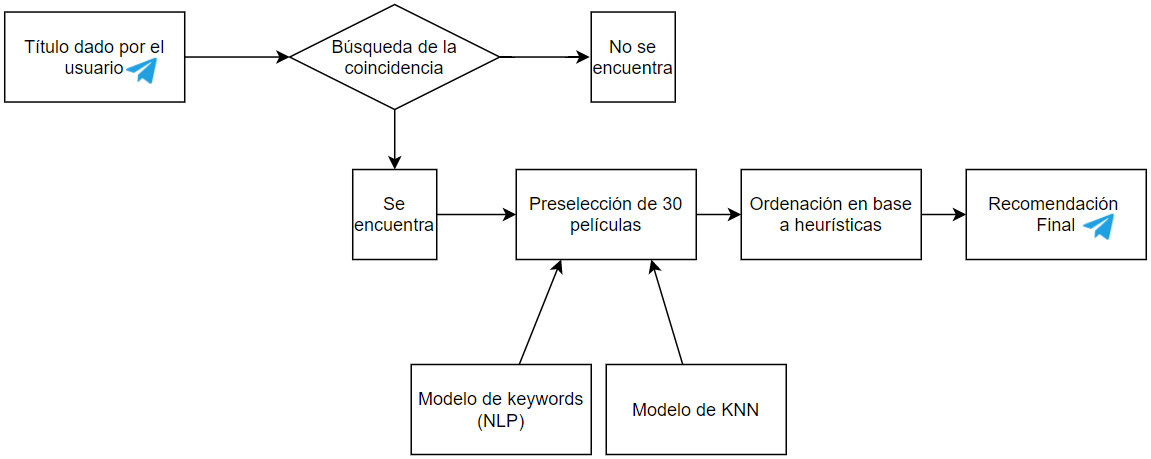
\includegraphics[width=12cm]{contenido/imagenes/FLujodattos.png}
    \caption{Flujo de la información en el sistema de recomendación.}
    \label{fig:flow}
\end{figure}


\subsection{Comparación con un sistema de filtrado colaborativo}

En la explicación de los tipos de sistemas de recomendación, ya se han enumerado las ventajas y desventajas de los dos tipos principales de sistemas. Sin embargo, una vez descrito con exactitud el sistema que hemos construido en esta memoria, consideramos oportuno el realizar una comparativa directa con otra implementación del un sistema de otro tipo; que en este caso será un sistema de filtrado colaborativo. De esta forma, se pondrá de manifiesto la aportación que realizamos al campo. Sin embargo, consideramos que nuestra aportación va más allá de una forma de crear un sistema de recomendación, por lo que en la \autoref{sec:reflexion} añadimos una pequeña reflexión sobre otras principios de diseño que hemos seguido que consideramos aportan al campo de los sistemas de recomendación.

En \cite{ilhami2014film} se realiza una implementación de un sistema de recomendación de filtrado colaborativo, aunque como puede verse en el artículo, cuentan con una cantidad de datos mucho mayor. En la \autoref{tab:compareSystems} se realiza una comparación entre el sistema propuesto en este artículo y el propuesto en este proyecto.

\begin{table}[H]
\centering
%\resizebox{0.8\textwidth}{!}{%
\begin{tabular}{p{0.3\linewidth}p{0.3\linewidth}p{0.3\linewidth}}
\hilne \textbf{Aspecto} & \textbf{Sistema de este TFE} & \textbf{Sistema propuesto en \cite{ilhami2014film}} \\ \hline 
Recomendaciones dependientes del usuario & El sistema recomienda películas independientemente del usuario que las solicita.                                                                                & Cada usuario está modelado de forma diferente, por lo que las recomendaciones sí que son únicas                                                                                                    \\
Nuevos usuarios y elementos              & Al ser independiente del usuario, la aparicion de nuevos usuarios no es un problema. Los nuevos contenidos serán recomendados una vez se rellenen sus metadatos & Puede haber problemas al tener usuarios que no hayan valorado ninguna película o películas que no hayan sido recomendadas. Es el problema denominado \textit{cold start}                           \\
Posibilidad de indexación                & Podemos tener precalculadas las recomendaciones, lo cual supone un gran ahorro de tiempo a la hora de servir las recomendaciones a los usuarios                 & Tener las recomendaciones precalculadas es muy costoso, al depender del producto entre usuarios y películas.                                                                                       \\
Agnosticismo                             & El sistema recomienda las películas independientemente de la plataforma en la que se encuentran, al contrario que sistemas de Netflix o Amazon                  & El conjunto de películas utilizado no proviene de una plataforma en cocnreto. Sin embargo, al usar votos de usuarios, es complicado introducir una película que no esté en la plataforma de votos. \\
Implementación Real                      & El proyecto de este trabajo se ha desarrollado de una forma \textit{end to end}, de forma que se ha generado un sistema de recomendación usable                 & El sistema de recomendacion creado es de laboratorio, no hay posibilidad de usarlo                                                                                                                
\end{tabular}%
%}
\caption{Comparación entre el sistema de recomendación propuesto en \cite{ilhami2014film} y en esta memoria.}
\label{tab:compareSystems}
\end{table}


\section{Reflexión}\label{sec:reflexion}

En esta sección del trabajo, queremos explicar algunas normas de diseño que se han seguido en la construcción de este sistema de recomendación. Resulta fácil pensar que este sistema difícilmente superará en términos de calidad de las recomendaciones a un sistema como el que puede tener implementado una empresa como Netflix o Amazon. Estas empresas tienen cientos de millones de usuarios y catálogos amplísimos, además de grandes equipos dedicados a crear estos sistemas de recomendación que tan lucrativos les son, pues son parte principal de su negocio. Estas empresas disponen también de información más allá de meras valoraciones de usuarios, como puede ser el tiempo de visionado de un producto antes de comprarlo, la cantidad de series que miran antes de elegir una... Datos que pueden ser muy relevantes a la hora de realizar una recomendación.\\

Consideramos que en este ambiente, somos los amantes del cine los que realmente perdemos. A la gente que le gusta el cine, que no es poca, realmente no le importa tanto dónde ver una película, sino que lo que quiere son recomendaciones significativas que le aporten valor. Es aquí donde creemos que nuestro sistema tiene uno de sus puntos fuertes. Un sistema como del de Netflix no tiene como objetivo el enriquecer tus conocimientos sobre cine, sino que por detrás existen otros intereses, menos explícitos, que son el mantenerte el máximo tiempo posible en sus plataformas, que gastes la mayor cantidad de dinero o que consumas contenidos con millones de dólares gastados en producción. Para ejemplificar esto, lanzamos una pregunta al aire: ¿cuándo fue la última vez que Netflix te recomendó una película de hace más de 20 años? Nosotros consideramos que no todo el público está orientado a consumir cine actual, y que mucha gente está dispuesta a buscar cómo consumir una película si cree que puede gustarle.\\

Además, en los últimos años, los usuarios se han vuelto cada vez más conscientes de los datos que dan a las plataformas que utilizan. Con la publicación en el año 2018 del Reglamento General de Protección de Datos, los ciudadanos de la UE vimos gratamente reforzados nuestros derechos respecto a nuestros datos personales. Plataformas como Amazon o Netflix almacenan todos los datos que les es posible, mientras que nuestra estrategia es una estrategia \textit{cero datos}, en la que intentamos no necesitar de ningun dato personal para poder realizar las recomendaciones.\\

Por tanto, dos normas de diseño que hemos mantenido en el desarrollo de este proyecto son las siguientes:

\begin{itemize}
    \item Agnosticismo: Nuestro sistema de recomendación es angóstico respecto a la plataforma en la que se consume el contenido. Por tanto, proveemos al sistema de una interfaz propia, multiplataforma, gratuita y de acceso libre como es Telegram para que los usuarios puedan realizar consultas al sistema. El objetivo primordial es dar al usuario las recomendaciones más significativas dentro de las posibilidades de los datos disponibles, entendiendo por significativa la película que más puede gustarle, sin tener en cuenta otros intereses que los del propio usuario.
    \item Cero datos: El sistema no almacena datos de los usuarios. Con el fin de proteger la privacidad de los usuarios, el sistema no registra de forma persistida las interacciones de cada usuario con el fin de modelarlo. Esta premisa tiene la desventaja de que es un sistema que no se puede mejorar con el uso, pero si puede mejorarse a través de la realización de modelados más eficientes de las películas.
\end{itemize}



,
        \chapter{Creación del sistema de recomendación}\label{chap:creacion}


En los capítulos anteriores se ha realizado una introducción al trabajo desarrollado en este proyecto, cuyo objetivo es la creación de un sistema de recomendación de películas basado en contenido. En dicha introducción, se ha realizado una justificación de la importancia de estos sistemas para las plataformas que alojan contenido así como para los usuarios.

Además, en el Capítulo \ref{chap:adq} se ha realizado el proceso de limpieza y preprocesameinto de los datos que, como se ha dicho, es fundamental para lograr un buen desempeño del modelo en esta parte.\\

Recordar que en este momento disponemos de un conjunto de datos de aproximadamente 5000 películas y que contiene las siguientes columnas para cada una de ellas: título, año, géneros, keywords, director, 3 intérpretes principales, votos, idioma, país, media de votos, duración y presupuesto.

\section{Funcionamiento del motor}

El motor partirá de una película dada por el usuario, a partir de la cual se buscan las más similares y le son recomendadas al usuario. La elección de las películas para recomendar se realizará en dos etapas diferenciadas:
\begin{enumerate}
    \item Elegir $N$ películas en base a una medida de similaridad, de forma que tengan un contenido parecido a la entrada dada por el usuario.
    \item Seleccionar las $M, M<N$ películas más populares de entre esas $N$ películas.
\end{enumerate}

Esta estrategia podría ser discutida y probablemente existan estrategias ligeramente superiores. Sin embargo, se ha escogido esta porque conceptualmente parece lógico que aunque se realice una preselección de $N \sim 30$ películas basándose en el contenido de las mismas y la similaridad en términos de keywords, se haga un segundo filtrado. Por lo general, las películas más populares serán mejores recomendaciones para los usuarios (siempre habrá usuarios mas snobs, pero lo que le gusta a mucha gente es probable que le guste al usuario). Es por eso que de la primera preselección de películas que se hace con las keywords, posteriormente se filtran con criterios más manuales. Es aquí donde se introduce ese conocimiento del dominio que tan importante es para obtener resultados buenos.


\subsection{Similaridad}

El primer paso en la construcción del motor de recomendación consiste en definir un criterio que aporte información sobre cómo de parecidas son dos películas. Partiendo de la película seleccionada por el usuario, se toma el director, los actores princpales, los géneros y las keywords de la película y se crea una matriz como la mostrada en \ref{tab:similarity}.

\begin{table}[H]
\centering
\begin{tabular}{|c|c|c|c|c|c|c|c|c|c|c|}
\hline
\textbf{\begin{tabular}[c]{@{}l@{}}movie\\ title\end{tabular}} &
  \textbf{director} &
  \textbf{actor 1} &
  \textbf{a2} &
  \textbf{a3} &
  \textbf{keyword 1} &
  \textbf{k2} &
  \textbf{genre1} &
  \textbf{g2} &
  \textbf{...} &
  \textbf{gk} \\ \hline
Film1  & $a_{11}$ & $a_{12}$ &  &  & ...      &  &  &  & ... & $a_{1q}$ \\ \hline
...    &          &          &  &  & ...      &  &  &  & ... &          \\ \hline
Film i & $a_{i1}$ & $a_{i2}$ &  &  & $a_{ij}$ &  &  &  & ... & $a_{iq}$ \\ \hline
...    &          &          &  &  & ...      &  &  &  & ... &          \\ \hline
Film p & $a_{p1}$ & $a_{p2}$ &  &  & ...      &  &  &  & ... & $a_{pq}$ \\ \hline
\end{tabular}
\caption{Matriz generada para el cálculo de la similaridad entre dos películas}
\label{tab:similarity}
\end{table}

En esta matriz, el elemento $ij$ toma el valor $0,1$ dependiendo de la correspondencia entre la película $i$ y el contenido de la columna $j$ (que depende de la película seleccionada). Por ejemplo, si "keyword1" está en la película $i$, tendremos $a_{ij} = 1$ y $0$ en otro caso. Una vez definida la matriz, se determina la distancia entre dos películas mediante

\begin{eqnarray}
d_{m, n} = \sqrt{  \sum_{i = 1}^{N} \left( a_{m,i}  - a_{n,i} \right)^2  } 
\end{eqnarray}

En este punto, únicamente tenemos que seleccionar las $N$ películas que son más cercanas a la entrada seleccionada por el usuario.

\subsection{Popularidad}

Atendiendo a la similaridad entre películas, seleccionamos una lista de $N$ películas. En este punto, seleccionaremos únicamente 5 películas. Para ello, damos una puntuación a cada entrada. Se computa la puntuación de acuerdo a estos tres criterios:
- La puntuación media.
- El siguiente ratio:
\begin{equation}
    R = \frac{\frac{votes - \bar{votes}}{\sigma_{votes}}}{\frac{gross - \bar{gross}}{\sigma_{gross}}}
\end{equation}

Que mide cuántos usuarios votaron la película respecto al presupuesto de la película, ambos datos normalizados.
- El año de lanzamiento.

Los dos primeros serán una medida directa de la popularidad de varias entradas. Para el tercer criterio, se introduce el año de lanzamiento. Se asume que las preferidas por la persona serán en la mayoría de los casos de la misma época.

A continuación, calculamos la puntuación de acuerdo a esta ecuación:

\begin{equation}
\mathrm{score} = puntuación^2 \times \phi_{\sigma_1, c_1} \times  \phi_{\sigma_2, c_2},
\label{eq:criteria}
\end{equation}

donde $\phi$ es una función gaussiana del tipo

\begin{equation}
\phi_{\sigma, c}(x) \propto \mathrm{exp}\left(-\frac{(x-c)^2}{2 \, \sigma^2}\right).
\end{equation}

En el caso del año se centra la gaussiana en el año de lanzamiento de la película elegida por el usuario y se elige $\sigma = 10$.\\

Además, como se verá más adelante, se realizarán algunas operaciones más con el fin de mejorar los resultados obtenidos.

\section{Definición de las funciones del motor}

En primer lugar es necesario extraer de la entrada seleccionada por el usuario, para ello se implementa la siguiente función:
\begin{lstlisting}[language=Python, caption= Variables utilizadas para la creación de la matriz.]
def entry_variables(df, id_entry): 
    """Calcula los valores tomados por las variables director_name, actor_[1,2,3]_name y plot_keywords para la
    película seleccionada por el usuario.

    Args:
        df (pd.DataFrame): DataFrame de películas
        id_entry (int): Id de la entrada seleccionada

    Returns:
        list: Lista que contiene los valores extraidos para la película seleccionada
    """
    
    col_labels = []    
    if pd.notnull(df['director_name'].iloc[id_entry]):
        for s in df['director_name'].iloc[id_entry].split('|'):
            col_labels.append(s)
            
    for i in range(3):
        column = 'actor_NUM_name'.replace('NUM', str(i+1))
        if pd.notnull(df[column].iloc[id_entry]):
            for s in df[column].iloc[id_entry].split('|'):
                col_labels.append(s)
                
    if pd.notnull(df['plot_keywords'].iloc[id_entry]):
        for s in df['plot_keywords'].iloc[id_entry].split('|'):
            col_labels.append(s)
    return col_labels
\end{lstlisting}

Una vez se tienen las variables con las que se calculará la distancia entre la película seleccionada por el usuario y las demás, se genera la matriz de $0$ y $1$ con una película por fila dependiendo de si coincide o no la información de ambas películas:

\begin{lstlisting}[language=Python, caption= Creación de la matriz de coordenadas de las películas.]
def add_variables(df, REF_VAR):
    """Añade al dataframe de películas las columnas dadas en REF_VAR (que serán el 
    director, etc de unapelícula) y las inicializa a 0 o 1 dependiendo de si la 
    película es del mismo director, tiene a ese actor, etc

    Args:
        df (pd.DataFrame): DataFrame de películas
        REF_VAR (list): Salida de aplicar entry_variables sobre el df y una película

    Returns:
        pd.DataFrame: DataFrame con las nuevas películas
    """
    for s in REF_VAR: 
        df[s] = pd.Series([0 for _ in range(len(df))])
    columns = ['genres', 'actor_1_name', 'actor_2_name',
                'actor_3_name', 'director_name', 'plot_keywords']
    for category in columns:
        for index, row in df.iterrows():
            if pd.isnull(row[category]): 
                continue
            for s in row[category].split('|'):
                if s in REF_VAR: df.set_value(index, s, 1)            
    return df
\end{lstlisting}

Con estas dos funciones ya definidas, podemos crear la función \texttt{recommend}, que será la que replace la selección de las $N$ películas más cercanas a la dada por el usuario. La métrica utilizada para evaluar cuales son las películas más cercanas es la distancia euclídea.

\begin{lstlisting}[language=Python, caption=Obtención de las 30 mejores películas dada una por el usuario.]
def recommend(df, id_entry, N = 31):
    """Crea una lista de N películas similares a las seleccionadas por el usuario

    Args:
        df (pd.DataFrame): DataFrame de películas
        id_entry (int): Id de la entrada seleccionada
        N (int, optional): Number of films recommended 
        (take into account that the nearest will be always itself). Defaults to 31.

    Returns:
        list: List of ids of films recommended
    """
    df_copy = df.copy(deep = True)    
    list_genres = set()
    for s in df['genres'].str.split('|').values:
        list_genres = list_genres.union(set(s))    

    # Creación de variables adicionales para comprobar la similaridad
    variables = entry_variables(df_copy, id_entry)
    variables += list(list_genres)
    df_new = add_variables(df_copy, variables)

    # Determinación de los vecinos más próximos: la distancia se calcula con las nuevas vairables
    X = df_new.as_matrix(variables)
    nbrs = NearestNeighbors(n_neighbors=N, algorithm='auto', metric='euclidean').fit(X)

    distances, indices = nbrs.kneighbors(X)    
    xtest = df_new.iloc[id_entry].as_matrix(variables)
    xtest = xtest.reshape(1, -1)

    distances, indices = nbrs.kneighbors(xtest)

    return indices[0][:]
\end{lstlisting}

Una vez se tienen las $N$ mejores películas, como se ha dicho anteriormente, se ordenan de forma descendente de acuerdo al criterio de la Ecuación\ref{eq:criteria} (implementado en la Función\ref{lst:criteria} utilizando la Función \texttt{extract\_parameters}:

\begin{lstlisting}[language=Python, caption=]
def extract_parameters(df, list_films, N = 31):
    """Extrae algunas variables del dataframe dado como entrada y devuelve la lista
    de N películas. Esta lista se ordena de acuerdo al criterio de la función 
    selection_criteria.

    Args:
        df ([type]): DataFrame de películas
        list_films (list): Lista con las n películas recomendadas
        N (int, optional): Number of films recommended. Defaults to 31.

    Returns:
        list: Películas recomendadas
    """
    films_parameters = ['_' for _ in range(N)]
    i = 0
    max_users = -1
    for index in list_films:
        film_parameters[i] = list(df.iloc[index][['movie_title', 'title_year',
                                        'vote_average', 
                                        'num_voted_users', 'gross']])
        film_parameters[i].append(index)
        max_users = max(max_users, film_parameters[i][4] )
        i += 1
    # The first element is the selected film itself
    title_main = film_parameters[0][0]
    ref_year  = film_parameters[0][1]
    votes_norm = (x[3] - df.num_voted_users.mean())/df.num_voted_users.std()
    gross_norm = (x[4] - df.gross.mean())/df.gross.std()

    
    film_parameters.sort(key = lambda x:selection_criteria(title_main,
                         ref_year, 
                         title = x[0], 
                         year = x[1],
                         score = x[2], 
                         ratio = votes_norm/gross_norm),
                         reverse = True)
    
    return parametres_films
\end{lstlisting}


\begin{lstlisting}[language=Python, caption=Criterios de selección para la elección de las mejores películas., label={lst:criteria}]
def selection_criteria(title_main, ref_year, title, year, score, ratio):
    """Calcula la puntuación de una película como recomendación de otra en base 
    a la similaridad de su título, la distancia temporal entre ambos lanzamientos
    y el número de votos de la película evaluada y la puntuación de la película.
    Además, la similitud entre títulos se tiene en cuenta para evitar la 
    recomendación de secuelas. Es decir, si dos películas tienen un nombre muy 
    similar, se desechara como recomendación.

    Args:
        title_main (str): Título de la película dada por el usuario
        ref_year (int): Año de lanzamiento de la película dada por el usuario
        title (str): Título de la película a evaluar
        year (int): Año de lanzamiento de la película a evaluar
        score (float): Votación media de la película a evaluar
        ratio (float): Ratio entre votos y presupuesto de la película

    Returns:
        float: Mark of the film given
    """
    if pd.notnull(ref_year):
        factor_1 = gaussian_filter(ref_year, year, 10)
    else:
        factor_1 = 1        

        
    if pd.notnull(votes):
        factor_2 = gaussian_filter(ratio, 0, 1)
    else:
        factor_2 = 0
        
    if sequel(title_main, title):
        mark = 0
        #print(f"Tenemos sequel entre {title_main} y {title}")
    else:
        mark = score * factor_1 * factor_2
    #print(f"'La nota de {title} es: {mark}'")
    return mark
\end{lstlisting}

Llegados a este punto, supóngase que el usuario ha elegido la película Harry Potter y la Piedra Filosofal. Sin ejecutar el recomendador y sin sonar demasiado raro, parece que las películas que recomendará el sistema, si no se modifica lo dicho hasta ahora, serán las demás películas de Harry Potter, ya que tendrán las mismas keywords o muy parecidas, compartirán actores y serán de la misma época. Sin embargo, estas películas sean probablemente conocidas por el usuario. Por tanto, se implementa la funcion \texttt{sequel}, que trata de ver, mediante lógica difusa y medidas como la distancia Levenshtein \cite{levenshtein}, que mide la distancia entre dos palabras en términos de los cambios necesarios para llegar de una a otra. La función \texttt{sequel}\ref{lst:sequel} servirá para filtrar los resultados dados al usuario.
\begin{lstlisting}[language=Python, caption=Determinación de si dos películas son o no secuelas y eliminarlas.]
def sequel(title_1, title_2):   
    """Compara los títulos de dos películas y devuelve si son similares o no

    Args:
        title_1 (str): Primer título
        title_2 (str): Segundo título

    Returns:
        bool: True if the films are sequels. False otherwise.
    """
    #print("$$$$$$$$$$$$$$$$$$$$$$")
    #print(title_1, "|",title_2)
    #print(fuzz.ratio(title_1, title_2) , fuzz.token_set_ratio(title_1, title_2))
    if fuzz.ratio(title_1.lower(), title_2.lower()) > 50 or fuzz.token_set_ratio(title_1.lower(), title_2.lower()) > 60:
        return True
    else:
        return False
def remove_sequels(film_selection):
    """Removes sequels from the list of films given

    Args:
        film_selection (list): Lista de películas de la que quitar las secuelas

    Returns:
        list: Lista sin secuelas
    """ 
    removed_from_selection = []
    for i, film_1 in enumerate(film_selection):
        for j, film_2 in enumerate(film_selection):
            if j <= i: continue 
            if sequel(film_1[0], film_2[0]): 
                last_film = film_2[0] if film_1[1] < film_2[1] else film_1[0]
                removed_from_selection.append(last_film)

    film_list = [film for film in film_selection if film[0] not in removed_from_selection]

    return film_list  
\end{lstlisting}

Finalmente, se implementa la función que se encarga de obtener estas 5 mejores películas:

\begin{lstlisting}[language=Python, caption=]
def add_to_selection(film_selection, parameters_films, N = 31):
    """Completa la lista film_selection que contiene 5 películas que se recomendarán
    al usuario. Las películas son seleccionadas de parameters_list y sólo se tienen
    en cuenta si el título es suficientemente distinto del de otras películas.

    Args:
        film_selection (list): Lista de películas
        parameters_films (list): Lista de parámetros
        N (int, optional): Películas a puntuar. Defaults to 31.
        M (int, optional): Películas a recomendar. Defaults to 5.

    Returns:
        list: films reselected
    """
    film_list = film_selection[:]
    icount = len(film_list)    
    for i in range(N):
        already_in_list = False
        for s in film_selection:
            if s[0] == parameters_films[i][0]: 
                already_in_list = True
            if sequel(parameters_films[i][0], s[0]): 
                already_in_list = True            
        if already_in_list: continue
            
        icount += 1
        if icount <= 5:
            film_list.append(parameters_films[i])
    return film_list
\end{lstlisting}

A modo de \textit{wrapper} de este flujo, la función \textt{find\_similarities} ejecuta todo el \textit{pipeline} de búsqueda de las películas recomendadas. Por ejemplo, para la película de Piratas del Caribe, el sistema realiza las siguientes recomendaciones:

\begin{enumerate}
    \item La comunidad del anillo
    \item Harry Potter y la cámara secreta
    \item X-Men: Días del futuro pasado
    \item El Hobbit, un viaje inesperado
    \item King Kong
\end{enumerate}

\begin{lstlisting}[language=Python, caption=Wrapper del pipeline de búsqueda de recomendaciones.]
def find_similarities(df, id_entry, del_sequels = True, verbose = False, N = 31):
    """Dado el id de una película busca las 5 mejores recomendaciones.

    Args:
        df (pd.DataFrame): [description]
        id_entry (int): [description]
        del_sequels (bool, optional): Borrar secuelas de las recomendaciones. Defaults to True.
        N (int, optional): Películas a evaluar. Defaults to 31.
        M (int, optional): Películas a recomendar. Defaults to 31.

    Returns:
        list: Selección de películas recomendadas
    """
    if verbose: 
        print(90*'_' + '\n' + "QUERY: films similar to id={} -> '{}'".format(id_entry,
                                df.iloc[id_entry]['movie_title']))
    list_films = recommend(df, id_entry, N)
    # Crear lista de N películas
    parameters_films = extract_parameters(df, list_films, N)
    #print("&&\n",parameters_films)
    # Seleccionar 5 películas de la  listaSelect 5 films from this list
    film_selection = []
    film_selection = add_to_selection(film_selection, parameters_films, N)
    #print("&&\n",film_selection)
    # Borrado de las secuelas
    if del_sequels: film_selection = remove_sequels(film_selection)
    # Añadir nuevas películas a la lista
    #print(film_selection)
    film_selection = add_to_selection(film_selection, parameters_films, N)
    selection_titles = []
    for i,s in enumerate(film_selection):
        selection_titles.append([s[0].replace(u'\xa0', u''), s[4]])
        if verbose: print("nº{:<2}     -> {:<30}".format(i+1, s[0]))

    return selection_titles
\end{lstlisting}

\section{Resumen}

En este capítulo, uno de los más importantes del proyecto, se ha creado el sistema de recomendación en sí, creando la medida de similaridad entre películas y realizando la seleccion de las mejores y se ha explicado el motivo de la inclusión de cada criterio de selección. Además, se ha mostrado un resultado del sistema a modo de ejemplo. La parte de explotación del resultado será tratada en el siguiente capítulo, en el que se introducirá el sistema en una API, abriendo la posibilidad de desplegar la solución en un entorno productivo utilizable por usuarios reales.,
        \chapter{Integración del sistema en una API}\label{chap:api}

Se ha visto que es una regla general en los trabajos de fin de estudios (no únicamente de UNIR, sino en general) orientados al Data Science y el análisis de datos la no creación de un entorno que podría denominarse productivo. Muchos de estos trabajos se centrar en realizar un análisis de los datos e implementar modelos predictivos, pero siempre en un entorno que podría considerarse ``de laboratorio''. Sin embargo, creemos que un TFE además de ser una forma de finalizar unos estudios, debería ser el inicio de aquello que viene después de ellos; el mundo real.\\

En este caso, el tema del TFE son los sistemas de recomendación de contenido. En este trabajo se ha revisado en primer lugar su necesidad en el entorno digital actual, en el que existen plataformas con muy variado contenido y usuarios que tienen que ser capaces de navegar por él. Además, se ha realizado una revisión teórica de los sistemas de recomendación, habiéndose explicado los principales tipos y sus aplicaciones. El caso de uso concreto que se ha llevado a cabo en este TFE ha sido relacionado con las películas. Se ha realizado un flujo completo de adquisición y preparación de los datos, a partir de diferentes datasets y se ha construido con ellos un sistema de recomendación. El sistema utiliza las palabras clave de cada película, el director, los actores, el año de lanzamiento y la popularidad de la película, para recomendar a un usuario películas dada una de referencia.\\

Como se ha explicado en el primer párrafo, consideramos que un TFE de desarrollo de software debería estar orientado a una implementación en el mundo real, en el que usuarios reales pudieran hacer uso del mismo. Este es un paso que suele dejarse indicado en los próximos pasos, no siendo así en este proyecto. Se implementará el sistema de recomendación en una REST API en Python utilizando la librería Flask y esta API será llamada por un bot de Telegram para responder a los usuarios.

\section{Telegram}

Telegram es una compañía de mensajería instantánea en la nube. Dispone de clientes para la mayoría de plataformas (Android, iOS, Windows Phone, macOS, linux...) y los usuarios pueden intercambiar mensajes, fotos, videos, audio, stickers o archivos de cualquier tipo. Además, la parte del cliente de Telegram es software libre (no así la parte de back-end), aunque en ocasiones la publicación no es inmediata. Como puede deducirse, Telegram es una compañía competidora de Whatsapp, aunque contiene características muy diferentes y atractivas.\\
\begin{figure}[H]
    \centering
    \captionsetup{width=7cm}
    
\includegraphics[width=5cm]{contenido/imagenes/Telegram-logo.jpg}
    \caption{Logo de la aplicación Telegram. Fuente: Wikipedia \cite{wiki:telegramImage}}
\end{figure}
Entre las innumerables características de Telegram, en este proyecto la de mayor importancia es la posibilidad de crear bots. Los bots de Telegram son aplicaciones de terceros que corren dentro de Telegram. Los usuarios pueden interactuar con los bots enviándoles mensajes y comandos. Entre las posibilidades de un bot se encuentran:
\begin{itemize}
    \item Obtener notificaciones personalizadas y noticias. Un bot puede actuar como un periódico, enviando contenido relevante para cada usuario de forma instantánea.
    \item Integrarse con otros servicios como GMail, GitHub o YouTube, permitiendo al usuario recibir, por ejemplo, notificaciones sobre cambios en sus repositorios.
    \item Aceptar pagos de usuarios de Telegram, gracias a la posibilidad de un bot de ofrecer servicios de pago.
    \item Creación de herramientas personalizadas, como alertas, previsiones meteorológicas, control domótico de la casa...
    \item Creación de juegos tanto de un jugador como para varios jugadores.
\end{itemize}

En resumen, existen bots para realizar prácticamente cualquier tarea, y en caso de que no exista, es posible crearlo si se dispone de las herramientas y los conocimientos adecuados; además de forma gratuita.\\

Los bots se distinguen de los humanos por su nombre (debe contener ``bot''), por no necesitar un teléfono para crear la cuenta y por no poder iniciar conversaciones con usuarios. Es el usuario quien debe iniciar una conversación con ellos.\\

En este caso particular, se utilizara Telegram como interfaz entre el usuario y el sistema de recomendación, tanto por sus cualidades como por su relativa facilidad de uso.\\

Para crear el bot, simplemente hay que iniciar una conversación con el bot \textit{@botfather} y enviar el comando \textit{$\backslash$newbot}, nos pedirá un nombre para el bot y un nombre de usuario, que tendrá que terminar en ``bot''. Una vez realizados estos pasos, se proporcionará el token que permite realizar modificaciones en el bot e interactuar a través de la API de Telegram. En la \autoref{fig:botfather} se muestra el proceso de creación del bot.

\begin{figure}[H]
    \centering
    \captionsetup{width=8cm}
    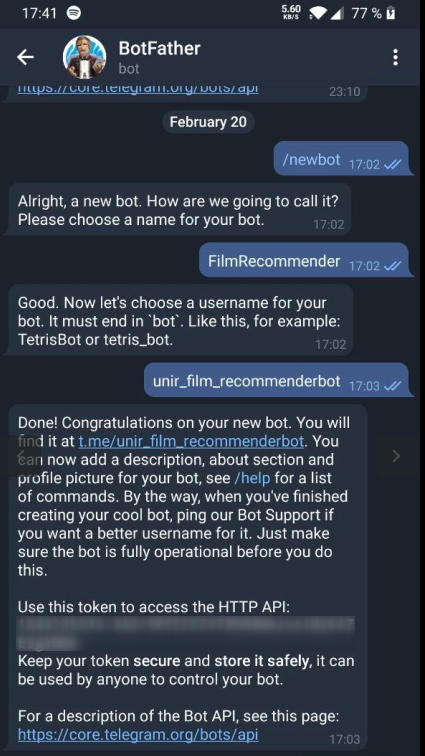
\includegraphics[width=6cm]{contenido/imagenes/botfather.png}
    \caption{Creación de un bot en Telegram mediante una conversación con el usuario \textit{@botfather}.}
    \label{fig:botfather}
\end{figure}


El funcionamiento del bot es el siguiente (puede obtenerse documentación más detallada en \cite{Telegram}):

\begin{enumerate}
    \item Se crea un webhook para que el bot envíe los mensajes que reciba a la URL que le proporcionemos, utilizando el siguiente método de la API: \url{https://api.telegram.org/bot<token>/setWebHook?url=<url_API>/telegram/}. De esta forma, cada vez que el bot reciba un mensaje, lo enviará a la URL de la API en formato JSON, para que la repuesta se procese.
    \item Se procesa el mensaje en la API creada (esta parte se detallará en la \autoref{sec:API}).
    \item Una vez la API ha procesado la petición del usuario y tiene la respuesta a enviar, se ejecuta la siguiente petición a la API de Telegram: \url{https://api.telegram.org/bot<token>/sendMessage?chat_id=<chat_id>&parse_mode=Markdown& text=<answer>}.
\end{enumerate}

Con estos simples pasos es posible crear un usuario de Telegram con el que cualquier usuario pueda interactuar, enviarle películas y obtener recomendaciones. Como se ha visto, la Telegram es un servicio con mucho potencial y relativamente sencillo y económico de implementar.

\section{Creación de la API en Python} \label{sec:API}

En la sección anterior se ha descrito de forma detallada el funcionamiento del chatbot desde el punto de vista de la API de Telegram, habiéndose explicado el funcionamiento de los bots en general y los pasos a seguir para crear un chatbot en esta plataforma. En esta sección se abordará el otro punto de vista, el de la API creada para implementar el sistema de recomendación.\\

Flask \cite{wiki:FlaskHelloWorld} es un micro framework web escrito en Python para crear aplicaciones web, es decir, páginas dinámicas, API, etc. Existen alternativas en Python como Django, que han sido descartados por ser demasiado complejos, en este caso se necesita crear una API relativamente sencilla. Es un framework rápido y sencillo.

\begin{figure}[H]
    \centering
    \captionsetup{width=7cm}
    \includesvg[width=9cm]{contenido/imagenes/flask}
    \caption{Logo del \textit{framework} Flask. Fuente: Wikipedia \cite{wiki:FlaskHelloWorld}}
\end{figure}

Mediante Flask se creará un servicio web que podrá ser llamado por el bot de Telegram, únicamente enviando a Telegram la URL del servicio Web y el token del bot. La API recibirá el mensaje, lo procesará y enviará al usuario la respuesta.\\

El ``hola mundo'' de Flask es el siguiente:

\begin{lstlisting}[language=Python, caption= {Aplicación Web básica creada con Flask. Se crea una API que devolverá la cadena de texto \textit{Hello world!} al ser invocada. Fuente: Wikipedia}]
from flask import Flask
app = Flask(__name__)

@app.route("/")
def hello():
    return "Hello world!"

if __name__ == "__main__":
    app.run(port = 8000)
\end{lstlisting}

Así, se tendría una aplicación web que en el puerto $8000$ devolvería ``Hello World''. Mediante los decoradores \texttt{@app.route()} se indica la ruta a través de la cual se entra a ese endpoint de la API.\\

La API se ejecutará en una Raspberry PI, debido a las ventajas que tiene en términos de coste frente a un servidor. Es de esperar que el servicio no tenga demasiadas solicitudes, por lo que tampoco tendrá problemas de volumen de peticiones. El problema es hacer que la API esté disponible a través de una URL. Para ello, dado que no se dispone de una IP estática ni de la posibilidad de abrir los puertos en el router, se utiliza el servicio \href{https://ngrok.com/}{Ngrok}. Ngrok es un servicio gratuito que publica un determinado puerto de localhost a través de una URL a través de un túnel.\\

Una vez explicado el funcionamiento, en el \autoref{lst:API}

\begin{lstlisting}[language=Python, label = {lst:API}, caption={Creación de la API del sistema de recomendación en Python usando Flask. En primer lugar se eliminan los posibles webhooks que existieran y se crea el nuevo con la URL a través de la cual pueda accederse a la API que estamos construyendo.}]
import requests
import time
import math
import os, json

from flask import Flask, request, json
from pyngrok import ngrok
from datetime import datetime
from configparser import ConfigParser
from datetime import timedelta
from recommendation import Recommendator
from utils import get_ngrok_url

# Lectura del fichero de configuración (Contiene el token)
config = ConfigParser()
config.read("telegram_config.ini")
telegram_token = config.get('mytokens', 'telegram')

# Creación del tunel seguro desde localhost
os.system('(./ngrok http 8000 &); exit')
time.sleep(2)

# Obtener la URL en la que está publicando el puerto 8000 ngrok
# (en el servicio gratuito es aleatoria)
url = get_ngrok_url()
url = url.replace('https://', '')
url = url.replace('http://', '')
print(url)


#Creación del webhook para que Telegram envíe los mensajes
deleteWebHook = 'https://api.telegram.org/bot' + telegram_token + '/deleteWebHook'
response_d = requests.get(deleteWebHook)
setWebHook = 'https://api.telegram.org/bot' + telegram_token + '/setWebHook?url=' + url+'/telegram/'
response = requests.get(setWebHook)
print(setWebHook)
print(response)
print(os.getcwd())

#Sistema de recomendación
recommendator = Recommendator()


app = Flask(__name__)
starting = math.floor(time.time())

@app.route('/')
def welcome():
    return 'Hola mundo'
@app.route('/telegram/', methods = ['POST', 'GET'])
def main ():
    
    # Mensaje recibido a través de TElegram y extracción de parámetros importantes
    recibido = dict(request.json)
    tiempo = recibido['message']['date']
    resta = tiempo-starting
    fecha_bien = datetime.fromtimestamp(starting).strftime("%A, %B %d, %Y %I:%M:%S")
    print(f'App started on {fecha_bien}')
    print(f"Message received {resta} seconds after starting.")
    if recibido["message"]["date"] > starting:
        # Caso en el que el mensaje se haya recibido con la aplicación operativa
        #(si no acumularía todos los mensajes y llegarían de repente)
        chat_id = str(recibido["message"]["chat"]['id'])
        usuario = recibido["message"]["chat"]["first_name"]
        mensaje = str(recibido["message"]["text"])
        print(usuario)
        print(recibido["message"]["text"])
        if mensaje != '/start':
            recommendation = recommendator.predict_from_string(mensaje)
            answer = recommendator.parse_response(recommendation)
        else:
            answer = """Welcome to the Film Recommendation Bot (built by Gonzalo Izaguirre).\n
            Just send us a title and we'll give you similar films."""
        
        send_text = 'https://api.telegram.org/bot' + telegram_token + '/sendMessage?chat_id=' + chat_id + '&parse_mode=Markdown&text=' + answer
        requests.get(send_text)
    return 'Hola Mundo'
if __name__ =='__main__':
    app.run(port = 8000)
\end{lstlisting}

En el \autoref{chap:creacion} se finalizó teniendo un sistema de recomendación que dado el id de una película, obtenía las películas recomendadas. Esto presenta un claro problema, ya que el usuario final no conocerá los ids, ya que son un identificador interno de la aplicación. Para obtener el id de una película a partir del mensaje del usuario se utiliza una estrategia similar a la seguida para saber si dos películas son secuelas o no. Utilizando lógica difusa y la distancia Levenshtein se compara la cadena de texto dada por el usuario con los títulos de las películas y se ordenan según su parecido. Si se supera un umbral determinado, se infiere que el título dado por el usuario se corresponde con el de mayor puntuación, y se buscan las recomendaciones utilizando ese id.

\begin{lstlisting}[language=Python, label = {lst:API}, caption= {Búsqueda del id de la película dada por el usuario. Estas funciones implementan la búsqueda de la película más parecida dentro de un umbral.}]
    @staticmethod
    def fuzzing(series_element, string):
        """Dadas dos cadenas de texto calcula la similaridad entre ambas. Se usa para cuando el usuario
        da como entrada una cadena de textopoder buscar la película a la que se refiere.
        Args:
            series_element (str): Cadena de texto 1
            string (str): Cadena de texto 2
        Returns:
            int: Similaridad entre las cadenas de texto
        """
        try:
            mark = 2/(1/fuzz.token_set_ratio(series_element.lower(), string.lower()) + 1/fuzz.ratio(series_element.lower(), string.lower()))
            return mark if mark > 60 else 0
        except:
            return 0

    def string_to_id(self, df, string):
        """Dada una cadena de texto se obtiene el id de la película que más se parece. Para ello se compara
        la cadena de texto con los títulos de las películas.
        Args:
            df (pd.DataFrame): DataFrame de películas
            string (str): Cadena de texto dada por el usuario.
        
        Returns:
            int: Id de la película encontrada.
        """
        df_2 = df.copy(deep = True)
        df_2["mark"] = df_2["movie_title"].apply(self.fuzzing , args = (string,))
        df_2.sort_values(by = ["mark", "title_year"], ascending = [False, True], inplace = True)
        #print("Parecido de la película introducida: ", df_2.iloc[0,-1])
        return df_2.index.values[0] if df_2.iloc[0,-1] > 60 else None
\end{lstlisting}

\section{Conversaciones de ejemplo}

En la \autoref{fig:TelegramResults} se muestran algunos ejemplos de conversaciones del chatbot de Telegram en las que el usuario aporta el título de una Película, y de una forma relativamente rápida ($\sim 10\ s$) el chatbot da las recomendaciones.\\


\begin{figure}[H]
\begin{subfigure}{.5\textwidth}
  \centering
  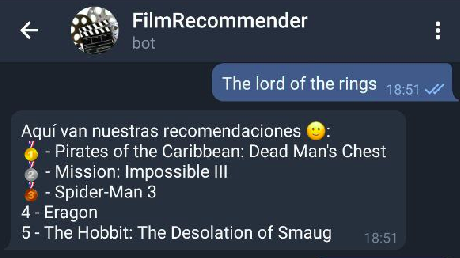
\includegraphics[width=.9\linewidth]{contenido/imagenes/sc1.png}
  \caption{Recomendaciones para El señor de los anillos.}
  \label{fig:sc1}
\end{subfigure}%
\begin{subfigure}{.5\textwidth}
  \centering
  
\includegraphics[width=.9\linewidth]{contenido/imagenes/sc2.png}
  \caption{Recomendaciónes para Eragon}
  \label{fig:sc2}
\end{subfigure}
\\
\begin{subfigure}{.5\textwidth}
  \centering
  
\includegraphics[width=.9\linewidth]{contenido/imagenes/sc3.png}
  \caption{Recomendaciones para El señor de los anillos.}
  \label{fig:sc3}
\end{subfigure}%
\begin{subfigure}{.5\textwidth}
  \centering
  
\includegraphics[width=.9\linewidth]{contenido/imagenes/sc4.png}
  \caption{Recomendación para El caso Bourne}
  \label{fig:sc4}
\end{subfigure}
\caption{Ejemplos de recomendaciones de películas dadas por el chatbot de Telegram. Le damos el título de una película y nos devuelve 5 recomendaciones ordenadas.}
\label{fig:TelegramResults}
\end{figure}

En este tipo de proyectos, resulta complicado evaluar los resultados. La calidad de las recomendaciones son algo bastante subjetivo, por lo que resulta complicado establecer una métrica de desempeño. Sin embargo, puede verse que las recomendaciones realizadas son relativamente acertadas, puesto que la temática y el género de las películas recomendadas es similar al de la dada.\\

\section{Código utilizado}

A lo largo del proyecto se ha ido adjuntando el código utilizado para cada una de las tareas, ya que creemos que resulta interesante conocer la estrategia seguida para tarea. Sin embargo, lo que se ha adjuntado son piezas de un Jupyter Notebook que genera el sistema de recomendación de forma interactiva (\autoref{app:notebook}. El código real se encuentra organizado en diferentes clases (preprocesado, imputación, recomendador, API...) para tener una estructura más organizada. El código puede consultarse en el repositorio de GitHub \url{https://github.com/gontxomde/RecommendationEngine} con una pequeña guía de despliegue y uso.\\

De la misma forma, a lo largo del proyecto, se han incluido en las funciones los denominados docstrings, que son formas estándar de definir el uso y los argumentos de una función en Python. La finalidad del uso de estos docstrings, además de hacer el código legible, es posibilitar el uso de Sphinx. Sphinx es un software que permite generar la documentación del código de forma automática, generando un documento html o latex fácilmente consultable. Además de en el repositorio antes mencionado, la documentación de la librería creada en este proyecto puede consultarse en el repositorio anteriormente mencionado.\\

Esperamos que esta forma de proceder a lo largo de la memoria haya facilitado la comprensión de los pasos seguidos para la creación del sistema de recomendación.


,
        \chapter{Conclusiones y trabajo futuro}\label{chap:resultados}
Este último bloque (habitualmente un capítulo; en ocasiones, dos capítulos complementarios) es habitual en todos los tipos de trabajos y presenta el resumen final de tu trabajo y debe servir para informar del alcance y relevancia de tu aportación.\par

Suele estructurarse empezando con un resumen del problema tratado, de cómo se ha abordado y de por qué la solución sería válida.
Es recomendable que incluya también un resumen de las contribuciones del trabajo, en el que relaciones las contribuciones y los resultados obtenidos con los objetivos que habías planteado para el trabajo, discutiendo hasta qué punto has conseguido resolver los objetivos planteados.\par

Finalmente, se suele dedicar una última sección a hablar de líneas de trabajo futuro que podrían aportar valor añadido al TFM realizado. La sección debería señalar las perspectivas de futuro que abre el trabajo desarrollado para el campo de estudio definido. En el fondo, debes justificar de qué modo puede emplearse la aportación que has desarrollado y en qué campos.

\begin{table}[H]
\centering
\begin{tabular}{llrr}
\toprule
{} &           column\_name &  missing\_count &  filling\_factor \\
\midrule
0  &              homepage &           3091 &           35.64 \\
1  &               tagline &            844 &           82.43 \\
2  &               country &            174 &           96.38 \\
3  &          actor\_3\_name &             93 &           98.06 \\
4  &              language &             86 &           98.21 \\
5  &          actor\_2\_name &             63 &           98.69 \\
6  &          actor\_1\_name &             53 &           98.90 \\
7  &         director\_name &             30 &           99.38 \\
8  &              overview &              3 &           99.94 \\
9  &              duration &              2 &           99.96 \\
10 &            title\_year &              1 &           99.98 \\
11 &          release\_date &              1 &           99.98 \\
12 &       num\_voted\_users &              0 &          100.00 \\
13 &          vote\_average &              0 &          100.00 \\
14 &           movie\_title &              0 &          100.00 \\
15 &                budget &              0 &          100.00 \\
16 &      spoken\_languages &              0 &          100.00 \\
17 &  production\_countries &              0 &          100.00 \\
18 &  production\_companies &              0 &          100.00 \\
19 &            popularity &              0 &          100.00 \\
20 &        original\_title &              0 &          100.00 \\
21 &         plot\_keywords &              0 &          100.00 \\
22 &                    id &              0 &          100.00 \\
23 &                genres &              0 &          100.00 \\
24 &                status &              0 &          100.00 \\
25 &                 gross &              0 &          100.00 \\
\bottomrule
\end{tabular}
\caption{Dimensiones de los datos de entrenamiento utilizados en \textbackslash{}cite\{Li2018\}}
\label{tab:datasets}
\end{table}

    %--- Apéndices y bibliografia ---%
    \cleardoublepage
\phantomsection
\addcontentsline{toc}{chapter}{Bibliography}
\printbibliography
    \begin{appendices}
        %Incluir aqui todos los apendices (carpeta contenido).
        \chapter{Notebook completo utilizado para la creación del sistema de recomendación}\label{app:notebook}




    \section{\texorpdfstring{\textbf{Film recommendation
engine}}{Film recommendation engine}}\label{film-recommendation-engine}

\emph{Gonzalo Izaguirre (diciembre 2019)} \_\_\_

El objetivo de este notebook es crear un motor de recomendación a partir
del contenido del fichero \texttt{movie\_metadata.csv}.Este dataset
contiene alrededor de 5000 películas y series, y su descripción ha sido
recogida de la base de datos de IMDB. Basicamente, el sistema funcionará
de la siguiente forma: después de que el usuario haya introducido el
nombre de una película que le haya gustado, el sistema seleccionará del
conjunto total 5 películas que agradarán al usuario al ser similares.
This dataset contains around 5000 movies and TV series, and their
description has been retrieved from the public IMDB database. Existen
tres tipos de filtros colaborativos: - Sistemas
\textbf{popularity-based}: los más simples de implementar, aunque los
más impersonales - Sistemas \textbf{content-based}: La recomendación se
basa en la descripción del producto - Sistemas \textbf{collaborative
filtering}: datos de diferentes usuarios dan recomendaciones basadas en
similaridades entre usuarios.

In the current case, since the dataset only describe the content of the
films and TV series, collaborative filtering is excluded and I will thus
build an engine that uses both the content and the popularity of the
entries.

En este caso, dado que el conjunto de datos solo describe el contenido
de las películas, no puede aplicarse el filtrado colaborativo. Se creará
un motor que usará tanto el contenido como la popularidad de las
entradas. \_\_\_ El notebook se organiza de la siguiente manera:

\textbf{1. Exploración} - 1.1 Keywords - 1.2 Factor de completitud:
Valores Faltantes - 1.3 Películas por año - 1.4 Géneros

\textbf{2. Limpieza} - 2.1 Entradas duplicadas - 2.2 Limpieza de
keywords * 2.2.1 Agrupamiento por lexema * 2.2.2 Agrupamiento por
sinónimos - 2.3 Correlaciones - 2.4 Valores faltantes * 2.4.1 Años
faltantes * 2.4.2 Extrayendo keywords del título * 2.4.3 Completado de
datos mediante regresión

\textbf{3. Recommendation Engine} - 3.1 Funcionamiento básico del motor
* 3.1.1 Similaridad * 3.1.2 Popularidad - 3.2 Definicion de las
funciones del motor de recomendación - 3.3 Realizando recomendaciones
interesantes - 3.4 Ejemplo de recomendación

\textbf{4. Conclusión: posibles mejoras y puntos a concretar}

    \begin{center}\rule{0.5\linewidth}{\linethickness}\end{center}

\subsection{1. Exploración}\label{exploraciuxf3n}

Se cargan todos los paquetes y el conjunto de datos. Se da información
sobre los tipos de las columnas y los datos faltantes.

    \begin{tcolorbox}[breakable, size=fbox, boxrule=1pt, pad at break*=1mm,colback=cellbackground, colframe=cellborder]
\prompt{In}{incolor}{1}{\hspace{4pt}}
\begin{Verbatim}[commandchars=\\\{\}]
\PY{c+c1}{\PYZsh{} new code block}
\PY{k+kn}{import} \PY{n+nn}{json}
\PY{k+kn}{import} \PY{n+nn}{pandas} \PY{k}{as} \PY{n+nn}{pd}
\end{Verbatim}
\end{tcolorbox}

    \begin{tcolorbox}[breakable, size=fbox, boxrule=1pt, pad at break*=1mm,colback=cellbackground, colframe=cellborder]
\prompt{In}{incolor}{2}{\hspace{4pt}}
\begin{Verbatim}[commandchars=\\\{\}]
\PY{c+c1}{\PYZsh{} new code block}
\PY{k}{def} \PY{n+nf}{load\PYZus{}tmdb\PYZus{}movies}\PY{p}{(}\PY{n}{path}\PY{p}{)}\PY{p}{:}
    \PY{l+s+sd}{\PYZdq{}\PYZdq{}\PYZdq{}}
\PY{l+s+sd}{    Función utilizada para cargar el dataset de las películas. Se transforma a fecha el campo de fecha de salida}
\PY{l+s+sd}{    y se cargan como listas los campos que están guardados como json.}

\PY{l+s+sd}{    Args:}
\PY{l+s+sd}{        path: Ruta hasta el archivo de tmdb\PYZus{}5000\PYZus{}movies.csv}

\PY{l+s+sd}{    Returns:}
\PY{l+s+sd}{        Dataframe de pandas con la información del csv}
\PY{l+s+sd}{    \PYZdq{}\PYZdq{}\PYZdq{}}
    \PY{n}{df} \PY{o}{=} \PY{n}{pd}\PY{o}{.}\PY{n}{read\PYZus{}csv}\PY{p}{(}\PY{n}{path}\PY{p}{)}
    \PY{n}{df}\PY{p}{[}\PY{l+s+s1}{\PYZsq{}}\PY{l+s+s1}{release\PYZus{}date}\PY{l+s+s1}{\PYZsq{}}\PY{p}{]} \PY{o}{=} \PY{n}{pd}\PY{o}{.}\PY{n}{to\PYZus{}datetime}\PY{p}{(}\PY{n}{df}\PY{p}{[}\PY{l+s+s1}{\PYZsq{}}\PY{l+s+s1}{release\PYZus{}date}\PY{l+s+s1}{\PYZsq{}}\PY{p}{]}\PY{p}{)}\PY{o}{.}\PY{n}{apply}\PY{p}{(}\PY{k}{lambda} \PY{n}{x}\PY{p}{:} \PY{n}{x}\PY{o}{.}\PY{n}{date}\PY{p}{(}\PY{p}{)}\PY{p}{)}
    \PY{n}{json\PYZus{}columns} \PY{o}{=} \PY{p}{[}\PY{l+s+s1}{\PYZsq{}}\PY{l+s+s1}{genres}\PY{l+s+s1}{\PYZsq{}}\PY{p}{,} \PY{l+s+s1}{\PYZsq{}}\PY{l+s+s1}{keywords}\PY{l+s+s1}{\PYZsq{}}\PY{p}{,} \PY{l+s+s1}{\PYZsq{}}\PY{l+s+s1}{production\PYZus{}countries}\PY{l+s+s1}{\PYZsq{}}\PY{p}{,} \PY{l+s+s1}{\PYZsq{}}\PY{l+s+s1}{production\PYZus{}companies}\PY{l+s+s1}{\PYZsq{}}\PY{p}{,} \PY{l+s+s1}{\PYZsq{}}\PY{l+s+s1}{spoken\PYZus{}languages}\PY{l+s+s1}{\PYZsq{}}\PY{p}{]}
    \PY{k}{for} \PY{n}{column} \PY{o+ow}{in} \PY{n}{json\PYZus{}columns}\PY{p}{:}
        \PY{n}{df}\PY{p}{[}\PY{n}{column}\PY{p}{]} \PY{o}{=} \PY{n}{df}\PY{p}{[}\PY{n}{column}\PY{p}{]}\PY{o}{.}\PY{n}{apply}\PY{p}{(}\PY{n}{json}\PY{o}{.}\PY{n}{loads}\PY{p}{)}
    \PY{k}{return} \PY{n}{df}


\PY{k}{def} \PY{n+nf}{load\PYZus{}tmdb\PYZus{}credits}\PY{p}{(}\PY{n}{path}\PY{p}{)}\PY{p}{:}
    \PY{l+s+sd}{\PYZdq{}\PYZdq{}\PYZdq{}}
\PY{l+s+sd}{    Función utilizada para cargar el dataset de los créditos. Se cargan como listas los campos que están guardado}

\PY{l+s+sd}{    Args:}
\PY{l+s+sd}{        path: Ruta hasta el archivo de tmdb\PYZus{}5000\PYZus{}credits.csv}

\PY{l+s+sd}{    Returns:}
\PY{l+s+sd}{        Dataframe de pandas con la información del csv}
\PY{l+s+sd}{    \PYZdq{}\PYZdq{}\PYZdq{}}
    \PY{n}{df} \PY{o}{=} \PY{n}{pd}\PY{o}{.}\PY{n}{read\PYZus{}csv}\PY{p}{(}\PY{n}{path}\PY{p}{)}
    \PY{n}{json\PYZus{}columns} \PY{o}{=} \PY{p}{[}\PY{l+s+s1}{\PYZsq{}}\PY{l+s+s1}{cast}\PY{l+s+s1}{\PYZsq{}}\PY{p}{,} \PY{l+s+s1}{\PYZsq{}}\PY{l+s+s1}{crew}\PY{l+s+s1}{\PYZsq{}}\PY{p}{]}
    \PY{k}{for} \PY{n}{column} \PY{o+ow}{in} \PY{n}{json\PYZus{}columns}\PY{p}{:}
        \PY{n}{df}\PY{p}{[}\PY{n}{column}\PY{p}{]} \PY{o}{=} \PY{n}{df}\PY{p}{[}\PY{n}{column}\PY{p}{]}\PY{o}{.}\PY{n}{apply}\PY{p}{(}\PY{n}{json}\PY{o}{.}\PY{n}{loads}\PY{p}{)}
    \PY{k}{return} \PY{n}{df}
\end{Verbatim}
\end{tcolorbox}

    \begin{tcolorbox}[breakable, size=fbox, boxrule=1pt, pad at break*=1mm,colback=cellbackground, colframe=cellborder]
\prompt{In}{incolor}{3}{\hspace{4pt}}
\begin{Verbatim}[commandchars=\\\{\}]
\PY{n}{LOST\PYZus{}COLUMNS} \PY{o}{=} \PY{p}{[}
    \PY{l+s+s1}{\PYZsq{}}\PY{l+s+s1}{actor\PYZus{}1\PYZus{}facebook\PYZus{}likes}\PY{l+s+s1}{\PYZsq{}}\PY{p}{,}
    \PY{l+s+s1}{\PYZsq{}}\PY{l+s+s1}{actor\PYZus{}2\PYZus{}facebook\PYZus{}likes}\PY{l+s+s1}{\PYZsq{}}\PY{p}{,}
    \PY{l+s+s1}{\PYZsq{}}\PY{l+s+s1}{actor\PYZus{}3\PYZus{}facebook\PYZus{}likes}\PY{l+s+s1}{\PYZsq{}}\PY{p}{,}
    \PY{l+s+s1}{\PYZsq{}}\PY{l+s+s1}{aspect\PYZus{}ratio}\PY{l+s+s1}{\PYZsq{}}\PY{p}{,}
    \PY{l+s+s1}{\PYZsq{}}\PY{l+s+s1}{cast\PYZus{}total\PYZus{}facebook\PYZus{}likes}\PY{l+s+s1}{\PYZsq{}}\PY{p}{,}
    \PY{l+s+s1}{\PYZsq{}}\PY{l+s+s1}{color}\PY{l+s+s1}{\PYZsq{}}\PY{p}{,}
    \PY{l+s+s1}{\PYZsq{}}\PY{l+s+s1}{content\PYZus{}rating}\PY{l+s+s1}{\PYZsq{}}\PY{p}{,}
    \PY{l+s+s1}{\PYZsq{}}\PY{l+s+s1}{director\PYZus{}facebook\PYZus{}likes}\PY{l+s+s1}{\PYZsq{}}\PY{p}{,}
    \PY{l+s+s1}{\PYZsq{}}\PY{l+s+s1}{facenumber\PYZus{}in\PYZus{}poster}\PY{l+s+s1}{\PYZsq{}}\PY{p}{,}
    \PY{l+s+s1}{\PYZsq{}}\PY{l+s+s1}{movie\PYZus{}facebook\PYZus{}likes}\PY{l+s+s1}{\PYZsq{}}\PY{p}{,}
    \PY{l+s+s1}{\PYZsq{}}\PY{l+s+s1}{movie\PYZus{}imdb\PYZus{}link}\PY{l+s+s1}{\PYZsq{}}\PY{p}{,}
    \PY{l+s+s1}{\PYZsq{}}\PY{l+s+s1}{num\PYZus{}critic\PYZus{}for\PYZus{}reviews}\PY{l+s+s1}{\PYZsq{}}\PY{p}{,}
    \PY{l+s+s1}{\PYZsq{}}\PY{l+s+s1}{num\PYZus{}user\PYZus{}for\PYZus{}reviews}\PY{l+s+s1}{\PYZsq{}}
                \PY{p}{]}

\PY{n}{TMDB\PYZus{}TO\PYZus{}IMDB\PYZus{}SIMPLE\PYZus{}EQUIVALENCIES} \PY{o}{=} \PY{p}{\PYZob{}}
    \PY{l+s+s1}{\PYZsq{}}\PY{l+s+s1}{budget}\PY{l+s+s1}{\PYZsq{}}\PY{p}{:} \PY{l+s+s1}{\PYZsq{}}\PY{l+s+s1}{budget}\PY{l+s+s1}{\PYZsq{}}\PY{p}{,}
    \PY{l+s+s1}{\PYZsq{}}\PY{l+s+s1}{genres}\PY{l+s+s1}{\PYZsq{}}\PY{p}{:} \PY{l+s+s1}{\PYZsq{}}\PY{l+s+s1}{genres}\PY{l+s+s1}{\PYZsq{}}\PY{p}{,}
    \PY{l+s+s1}{\PYZsq{}}\PY{l+s+s1}{revenue}\PY{l+s+s1}{\PYZsq{}}\PY{p}{:} \PY{l+s+s1}{\PYZsq{}}\PY{l+s+s1}{gross}\PY{l+s+s1}{\PYZsq{}}\PY{p}{,}
    \PY{l+s+s1}{\PYZsq{}}\PY{l+s+s1}{title}\PY{l+s+s1}{\PYZsq{}}\PY{p}{:} \PY{l+s+s1}{\PYZsq{}}\PY{l+s+s1}{movie\PYZus{}title}\PY{l+s+s1}{\PYZsq{}}\PY{p}{,}
    \PY{l+s+s1}{\PYZsq{}}\PY{l+s+s1}{runtime}\PY{l+s+s1}{\PYZsq{}}\PY{p}{:} \PY{l+s+s1}{\PYZsq{}}\PY{l+s+s1}{duration}\PY{l+s+s1}{\PYZsq{}}\PY{p}{,}
    \PY{l+s+s1}{\PYZsq{}}\PY{l+s+s1}{original\PYZus{}language}\PY{l+s+s1}{\PYZsq{}}\PY{p}{:} \PY{l+s+s1}{\PYZsq{}}\PY{l+s+s1}{language}\PY{l+s+s1}{\PYZsq{}}\PY{p}{,}  \PY{c+c1}{\PYZsh{} it\PYZsq{}s possible that spoken\PYZus{}languages would be a better match}
    \PY{l+s+s1}{\PYZsq{}}\PY{l+s+s1}{keywords}\PY{l+s+s1}{\PYZsq{}}\PY{p}{:} \PY{l+s+s1}{\PYZsq{}}\PY{l+s+s1}{plot\PYZus{}keywords}\PY{l+s+s1}{\PYZsq{}}\PY{p}{,}
    \PY{l+s+s1}{\PYZsq{}}\PY{l+s+s1}{vote\PYZus{}count}\PY{l+s+s1}{\PYZsq{}}\PY{p}{:} \PY{l+s+s1}{\PYZsq{}}\PY{l+s+s1}{num\PYZus{}voted\PYZus{}users}\PY{l+s+s1}{\PYZsq{}}\PY{p}{,}
                                         \PY{p}{\PYZcb{}}

\PY{n}{IMDB\PYZus{}COLUMNS\PYZus{}TO\PYZus{}REMAP} \PY{o}{=} \PY{p}{\PYZob{}}\PY{l+s+s1}{\PYZsq{}}\PY{l+s+s1}{imdb\PYZus{}score}\PY{l+s+s1}{\PYZsq{}}\PY{p}{:} \PY{l+s+s1}{\PYZsq{}}\PY{l+s+s1}{vote\PYZus{}average}\PY{l+s+s1}{\PYZsq{}}\PY{p}{\PYZcb{}}
\end{Verbatim}
\end{tcolorbox}

    \begin{tcolorbox}[breakable, size=fbox, boxrule=1pt, pad at break*=1mm,colback=cellbackground, colframe=cellborder]
\prompt{In}{incolor}{4}{\hspace{4pt}}
\begin{Verbatim}[commandchars=\\\{\}]
\PY{o}{\PYZpc{}}\PY{k}{config} IPCompleter.greedy=True
\end{Verbatim}
\end{tcolorbox}

    \begin{tcolorbox}[breakable, size=fbox, boxrule=1pt, pad at break*=1mm,colback=cellbackground, colframe=cellborder]
\prompt{In}{incolor}{5}{\hspace{4pt}}
\begin{Verbatim}[commandchars=\\\{\}]
\PY{k}{def} \PY{n+nf}{safe\PYZus{}access}\PY{p}{(}\PY{n}{container}\PY{p}{,} \PY{n}{index\PYZus{}values}\PY{p}{)}\PY{p}{:}
    \PY{l+s+sd}{\PYZdq{}\PYZdq{}\PYZdq{}}
\PY{l+s+sd}{    Función para acceder de forma segura a valores. En caso de que no se encuentre uno de ellos, se devuelve NaN}
\PY{l+s+sd}{    en vez de lanzar un error.}

\PY{l+s+sd}{    Args:}
\PY{l+s+sd}{        container: Lista/ contenedor de la que quieren extraerse los valores}
\PY{l+s+sd}{        index\PYZus{}values: Lista de índices a extraer del contenedor}

\PY{l+s+sd}{    Returns:}
\PY{l+s+sd}{        }
\PY{l+s+sd}{    \PYZdq{}\PYZdq{}\PYZdq{}}
    \PY{n}{result} \PY{o}{=} \PY{n}{container}
    \PY{k}{try}\PY{p}{:}
        \PY{k}{for} \PY{n}{idx} \PY{o+ow}{in} \PY{n}{index\PYZus{}values}\PY{p}{:}
            \PY{n}{result} \PY{o}{=} \PY{n}{result}\PY{p}{[}\PY{n}{idx}\PY{p}{]}
        \PY{k}{return} \PY{n}{result}
    \PY{k}{except} \PY{n+ne}{IndexError} \PY{o+ow}{or} \PY{n+ne}{KeyError}\PY{p}{:}
        \PY{k}{return} \PY{n}{pd}\PY{o}{.}\PY{n}{np}\PY{o}{.}\PY{n}{nan}


\PY{k}{def} \PY{n+nf}{get\PYZus{}director}\PY{p}{(}\PY{n}{crew\PYZus{}data}\PY{p}{)}\PY{p}{:}
    \PY{l+s+sd}{\PYZdq{}\PYZdq{}\PYZdq{}Devuelve el director dado un json con toda la composición del equipo de la película.}
\PY{l+s+sd}{    }
\PY{l+s+sd}{    Arguments:}
\PY{l+s+sd}{        crew\PYZus{}data \PYZhy{}\PYZhy{} JSON con el equipo que ha realizado la película}
\PY{l+s+sd}{    }
\PY{l+s+sd}{    Returns:}
\PY{l+s+sd}{        str \PYZhy{}\PYZhy{} director de la película}
\PY{l+s+sd}{    \PYZdq{}\PYZdq{}\PYZdq{}}
    \PY{n}{directors} \PY{o}{=} \PY{p}{[}\PY{n}{x}\PY{p}{[}\PY{l+s+s1}{\PYZsq{}}\PY{l+s+s1}{name}\PY{l+s+s1}{\PYZsq{}}\PY{p}{]} \PY{k}{for} \PY{n}{x} \PY{o+ow}{in} \PY{n}{crew\PYZus{}data} \PY{k}{if} \PY{n}{x}\PY{p}{[}\PY{l+s+s1}{\PYZsq{}}\PY{l+s+s1}{job}\PY{l+s+s1}{\PYZsq{}}\PY{p}{]} \PY{o}{==} \PY{l+s+s1}{\PYZsq{}}\PY{l+s+s1}{Director}\PY{l+s+s1}{\PYZsq{}}\PY{p}{]}
    \PY{k}{return} \PY{n}{safe\PYZus{}access}\PY{p}{(}\PY{n}{directors}\PY{p}{,} \PY{p}{[}\PY{l+m+mi}{0}\PY{p}{]}\PY{p}{)}


\PY{k}{def} \PY{n+nf}{pipe\PYZus{}flatten\PYZus{}names}\PY{p}{(}\PY{n}{keywords}\PY{p}{)}\PY{p}{:}
    \PY{l+s+sd}{\PYZdq{}\PYZdq{}\PYZdq{}Obtiene una lista con las keywords separadas por un pipe | extrayéndolas del json.}
\PY{l+s+sd}{    }
\PY{l+s+sd}{    Arguments:}
\PY{l+s+sd}{        keywords \PYZhy{}\PYZhy{} JSON de keywords de la película}
\PY{l+s+sd}{    }
\PY{l+s+sd}{    Returns:}
\PY{l+s+sd}{        str \PYZhy{}\PYZhy{} keywords de la película juntas}
\PY{l+s+sd}{    \PYZdq{}\PYZdq{}\PYZdq{}}
    \PY{k}{return} \PY{l+s+s1}{\PYZsq{}}\PY{l+s+s1}{|}\PY{l+s+s1}{\PYZsq{}}\PY{o}{.}\PY{n}{join}\PY{p}{(}\PY{p}{[}\PY{n}{x}\PY{p}{[}\PY{l+s+s1}{\PYZsq{}}\PY{l+s+s1}{name}\PY{l+s+s1}{\PYZsq{}}\PY{p}{]} \PY{k}{for} \PY{n}{x} \PY{o+ow}{in} \PY{n}{keywords}\PY{p}{]}\PY{p}{)}


\PY{k}{def} \PY{n+nf}{convert\PYZus{}to\PYZus{}original\PYZus{}format}\PY{p}{(}\PY{n}{movies}\PY{p}{,} \PY{n}{credits}\PY{p}{)}\PY{p}{:}
    \PY{l+s+sd}{\PYZdq{}\PYZdq{}\PYZdq{}Aplica una serie de funciones para añadir información al dataset de películas a partir del}
\PY{l+s+sd}{    conjunto de datos de créditos}
\PY{l+s+sd}{    }
\PY{l+s+sd}{    Arguments:}
\PY{l+s+sd}{        movies \PYZhy{}\PYZhy{} DataFrame obtenido de leer el archivo de películas}
\PY{l+s+sd}{        credits \PYZhy{}\PYZhy{} DataFrame obtenido de leet el archivo de créditos}
\PY{l+s+sd}{    }
\PY{l+s+sd}{    Returns:}
\PY{l+s+sd}{        DataFrame \PYZhy{}\PYZhy{} Datos obtenidos de cruzar ambos conjuntos de datos.}
\PY{l+s+sd}{    \PYZdq{}\PYZdq{}\PYZdq{}}
    \PY{n}{tmdb\PYZus{}movies} \PY{o}{=} \PY{n}{movies}\PY{o}{.}\PY{n}{copy}\PY{p}{(}\PY{p}{)}
    \PY{n}{tmdb\PYZus{}movies}\PY{o}{.}\PY{n}{rename}\PY{p}{(}\PY{n}{columns}\PY{o}{=}\PY{n}{TMDB\PYZus{}TO\PYZus{}IMDB\PYZus{}SIMPLE\PYZus{}EQUIVALENCIES}\PY{p}{,} \PY{n}{inplace}\PY{o}{=}\PY{k+kc}{True}\PY{p}{)}
    \PY{n}{tmdb\PYZus{}movies}\PY{p}{[}\PY{l+s+s1}{\PYZsq{}}\PY{l+s+s1}{title\PYZus{}year}\PY{l+s+s1}{\PYZsq{}}\PY{p}{]} \PY{o}{=} \PY{n}{pd}\PY{o}{.}\PY{n}{to\PYZus{}datetime}\PY{p}{(}\PY{n}{tmdb\PYZus{}movies}\PY{p}{[}\PY{l+s+s1}{\PYZsq{}}\PY{l+s+s1}{release\PYZus{}date}\PY{l+s+s1}{\PYZsq{}}\PY{p}{]}\PY{p}{)}\PY{o}{.}\PY{n}{apply}\PY{p}{(}\PY{k}{lambda} \PY{n}{x}\PY{p}{:} \PY{n}{x}\PY{o}{.}\PY{n}{year}\PY{p}{)}
    \PY{c+c1}{\PYZsh{} I\PYZsq{}m assuming that the first production country is equivalent, but have not been able to validate this}
    \PY{n}{tmdb\PYZus{}movies}\PY{p}{[}\PY{l+s+s1}{\PYZsq{}}\PY{l+s+s1}{country}\PY{l+s+s1}{\PYZsq{}}\PY{p}{]} \PY{o}{=} \PY{n}{tmdb\PYZus{}movies}\PY{p}{[}\PY{l+s+s1}{\PYZsq{}}\PY{l+s+s1}{production\PYZus{}countries}\PY{l+s+s1}{\PYZsq{}}\PY{p}{]}\PY{o}{.}\PY{n}{apply}\PY{p}{(}\PY{k}{lambda} \PY{n}{x}\PY{p}{:} \PY{n}{safe\PYZus{}access}\PY{p}{(}\PY{n}{x}\PY{p}{,} \PY{p}{[}\PY{l+m+mi}{0}\PY{p}{,} \PY{l+s+s1}{\PYZsq{}}\PY{l+s+s1}{name}\PY{l+s+s1}{\PYZsq{}}\PY{p}{]}\PY{p}{)}\PY{p}{)}
    \PY{n}{tmdb\PYZus{}movies}\PY{p}{[}\PY{l+s+s1}{\PYZsq{}}\PY{l+s+s1}{language}\PY{l+s+s1}{\PYZsq{}}\PY{p}{]} \PY{o}{=} \PY{n}{tmdb\PYZus{}movies}\PY{p}{[}\PY{l+s+s1}{\PYZsq{}}\PY{l+s+s1}{spoken\PYZus{}languages}\PY{l+s+s1}{\PYZsq{}}\PY{p}{]}\PY{o}{.}\PY{n}{apply}\PY{p}{(}\PY{k}{lambda} \PY{n}{x}\PY{p}{:} \PY{n}{safe\PYZus{}access}\PY{p}{(}\PY{n}{x}\PY{p}{,} \PY{p}{[}\PY{l+m+mi}{0}\PY{p}{,} \PY{l+s+s1}{\PYZsq{}}\PY{l+s+s1}{name}\PY{l+s+s1}{\PYZsq{}}\PY{p}{]}\PY{p}{)}\PY{p}{)}
    \PY{n}{tmdb\PYZus{}movies}\PY{p}{[}\PY{l+s+s1}{\PYZsq{}}\PY{l+s+s1}{director\PYZus{}name}\PY{l+s+s1}{\PYZsq{}}\PY{p}{]} \PY{o}{=} \PY{n}{credits}\PY{p}{[}\PY{l+s+s1}{\PYZsq{}}\PY{l+s+s1}{crew}\PY{l+s+s1}{\PYZsq{}}\PY{p}{]}\PY{o}{.}\PY{n}{apply}\PY{p}{(}\PY{n}{get\PYZus{}director}\PY{p}{)}
    \PY{n}{tmdb\PYZus{}movies}\PY{p}{[}\PY{l+s+s1}{\PYZsq{}}\PY{l+s+s1}{actor\PYZus{}1\PYZus{}name}\PY{l+s+s1}{\PYZsq{}}\PY{p}{]} \PY{o}{=} \PY{n}{credits}\PY{p}{[}\PY{l+s+s1}{\PYZsq{}}\PY{l+s+s1}{cast}\PY{l+s+s1}{\PYZsq{}}\PY{p}{]}\PY{o}{.}\PY{n}{apply}\PY{p}{(}\PY{k}{lambda} \PY{n}{x}\PY{p}{:} \PY{n}{safe\PYZus{}access}\PY{p}{(}\PY{n}{x}\PY{p}{,} \PY{p}{[}\PY{l+m+mi}{1}\PY{p}{,} \PY{l+s+s1}{\PYZsq{}}\PY{l+s+s1}{name}\PY{l+s+s1}{\PYZsq{}}\PY{p}{]}\PY{p}{)}\PY{p}{)}
    \PY{n}{tmdb\PYZus{}movies}\PY{p}{[}\PY{l+s+s1}{\PYZsq{}}\PY{l+s+s1}{actor\PYZus{}2\PYZus{}name}\PY{l+s+s1}{\PYZsq{}}\PY{p}{]} \PY{o}{=} \PY{n}{credits}\PY{p}{[}\PY{l+s+s1}{\PYZsq{}}\PY{l+s+s1}{cast}\PY{l+s+s1}{\PYZsq{}}\PY{p}{]}\PY{o}{.}\PY{n}{apply}\PY{p}{(}\PY{k}{lambda} \PY{n}{x}\PY{p}{:} \PY{n}{safe\PYZus{}access}\PY{p}{(}\PY{n}{x}\PY{p}{,} \PY{p}{[}\PY{l+m+mi}{2}\PY{p}{,} \PY{l+s+s1}{\PYZsq{}}\PY{l+s+s1}{name}\PY{l+s+s1}{\PYZsq{}}\PY{p}{]}\PY{p}{)}\PY{p}{)}
    \PY{n}{tmdb\PYZus{}movies}\PY{p}{[}\PY{l+s+s1}{\PYZsq{}}\PY{l+s+s1}{actor\PYZus{}3\PYZus{}name}\PY{l+s+s1}{\PYZsq{}}\PY{p}{]} \PY{o}{=} \PY{n}{credits}\PY{p}{[}\PY{l+s+s1}{\PYZsq{}}\PY{l+s+s1}{cast}\PY{l+s+s1}{\PYZsq{}}\PY{p}{]}\PY{o}{.}\PY{n}{apply}\PY{p}{(}\PY{k}{lambda} \PY{n}{x}\PY{p}{:} \PY{n}{safe\PYZus{}access}\PY{p}{(}\PY{n}{x}\PY{p}{,} \PY{p}{[}\PY{l+m+mi}{3}\PY{p}{,} \PY{l+s+s1}{\PYZsq{}}\PY{l+s+s1}{name}\PY{l+s+s1}{\PYZsq{}}\PY{p}{]}\PY{p}{)}\PY{p}{)}
    \PY{n}{tmdb\PYZus{}movies}\PY{p}{[}\PY{l+s+s1}{\PYZsq{}}\PY{l+s+s1}{genres}\PY{l+s+s1}{\PYZsq{}}\PY{p}{]} \PY{o}{=} \PY{n}{tmdb\PYZus{}movies}\PY{p}{[}\PY{l+s+s1}{\PYZsq{}}\PY{l+s+s1}{genres}\PY{l+s+s1}{\PYZsq{}}\PY{p}{]}\PY{o}{.}\PY{n}{apply}\PY{p}{(}\PY{n}{pipe\PYZus{}flatten\PYZus{}names}\PY{p}{)}
    \PY{n}{tmdb\PYZus{}movies}\PY{p}{[}\PY{l+s+s1}{\PYZsq{}}\PY{l+s+s1}{plot\PYZus{}keywords}\PY{l+s+s1}{\PYZsq{}}\PY{p}{]} \PY{o}{=} \PY{n}{tmdb\PYZus{}movies}\PY{p}{[}\PY{l+s+s1}{\PYZsq{}}\PY{l+s+s1}{plot\PYZus{}keywords}\PY{l+s+s1}{\PYZsq{}}\PY{p}{]}\PY{o}{.}\PY{n}{apply}\PY{p}{(}\PY{n}{pipe\PYZus{}flatten\PYZus{}names}\PY{p}{)}
    \PY{k}{return} \PY{n}{tmdb\PYZus{}movies}
\end{Verbatim}
\end{tcolorbox}

    \begin{tcolorbox}[breakable, size=fbox, boxrule=1pt, pad at break*=1mm,colback=cellbackground, colframe=cellborder]
\prompt{In}{incolor}{6}{\hspace{4pt}}
\begin{Verbatim}[commandchars=\\\{\}]
\PY{k+kn}{import} \PY{n+nn}{pandas} \PY{k}{as} \PY{n+nn}{pd}
\PY{k+kn}{import} \PY{n+nn}{numpy} \PY{k}{as} \PY{n+nn}{np}
\PY{k+kn}{import} \PY{n+nn}{matplotlib} \PY{k}{as} \PY{n+nn}{mpl}
\PY{k+kn}{import} \PY{n+nn}{matplotlib}\PY{n+nn}{.}\PY{n+nn}{pyplot} \PY{k}{as} \PY{n+nn}{plt}
\PY{k+kn}{import} \PY{n+nn}{seaborn} \PY{k}{as} \PY{n+nn}{sns}
\PY{k+kn}{import} \PY{n+nn}{math}\PY{o}{,} \PY{n+nn}{nltk}\PY{o}{,} \PY{n+nn}{warnings}
\PY{k+kn}{from} \PY{n+nn}{nltk}\PY{n+nn}{.}\PY{n+nn}{corpus} \PY{k+kn}{import} \PY{n}{wordnet}
\PY{k+kn}{from} \PY{n+nn}{sklearn} \PY{k+kn}{import} \PY{n}{linear\PYZus{}model}
\PY{k+kn}{from} \PY{n+nn}{sklearn}\PY{n+nn}{.}\PY{n+nn}{neighbors} \PY{k+kn}{import} \PY{n}{NearestNeighbors}
\PY{k+kn}{from} \PY{n+nn}{fuzzywuzzy} \PY{k+kn}{import} \PY{n}{fuzz}
\PY{k+kn}{from} \PY{n+nn}{wordcloud} \PY{k+kn}{import} \PY{n}{WordCloud}\PY{p}{,} \PY{n}{STOPWORDS}
\PY{n}{plt}\PY{o}{.}\PY{n}{rcParams}\PY{p}{[}\PY{l+s+s2}{\PYZdq{}}\PY{l+s+s2}{patch.force\PYZus{}edgecolor}\PY{l+s+s2}{\PYZdq{}}\PY{p}{]} \PY{o}{=} \PY{k+kc}{True}
\PY{n}{plt}\PY{o}{.}\PY{n}{style}\PY{o}{.}\PY{n}{use}\PY{p}{(}\PY{l+s+s1}{\PYZsq{}}\PY{l+s+s1}{fivethirtyeight}\PY{l+s+s1}{\PYZsq{}}\PY{p}{)}
\PY{n}{mpl}\PY{o}{.}\PY{n}{rc}\PY{p}{(}\PY{l+s+s1}{\PYZsq{}}\PY{l+s+s1}{patch}\PY{l+s+s1}{\PYZsq{}}\PY{p}{,} \PY{n}{edgecolor} \PY{o}{=} \PY{l+s+s1}{\PYZsq{}}\PY{l+s+s1}{dimgray}\PY{l+s+s1}{\PYZsq{}}\PY{p}{,} \PY{n}{linewidth}\PY{o}{=}\PY{l+m+mi}{1}\PY{p}{)}
\PY{k+kn}{from} \PY{n+nn}{IPython}\PY{n+nn}{.}\PY{n+nn}{core}\PY{n+nn}{.}\PY{n+nn}{interactiveshell} \PY{k+kn}{import} \PY{n}{InteractiveShell}
\PY{n}{InteractiveShell}\PY{o}{.}\PY{n}{ast\PYZus{}node\PYZus{}interactivity} \PY{o}{=} \PY{l+s+s2}{\PYZdq{}}\PY{l+s+s2}{last\PYZus{}expr}\PY{l+s+s2}{\PYZdq{}}
\PY{n}{pd}\PY{o}{.}\PY{n}{options}\PY{o}{.}\PY{n}{display}\PY{o}{.}\PY{n}{max\PYZus{}columns} \PY{o}{=} \PY{l+m+mi}{50}
\PY{o}{\PYZpc{}}\PY{k}{matplotlib} inline
\PY{n}{warnings}\PY{o}{.}\PY{n}{filterwarnings}\PY{p}{(}\PY{l+s+s1}{\PYZsq{}}\PY{l+s+s1}{ignore}\PY{l+s+s1}{\PYZsq{}}\PY{p}{)}

\PY{c+c1}{\PYZsh{}Definimos la función a utilizar para obtener el lexema de las palabras.}
\PY{n}{PS} \PY{o}{=} \PY{n}{nltk}\PY{o}{.}\PY{n}{stem}\PY{o}{.}\PY{n}{PorterStemmer}\PY{p}{(}\PY{p}{)}
\PY{c+c1}{\PYZsh{}\PYZus{}\PYZus{}\PYZus{}\PYZus{}\PYZus{}\PYZus{}\PYZus{}\PYZus{}\PYZus{}\PYZus{}\PYZus{}\PYZus{}\PYZus{}\PYZus{}\PYZus{}\PYZus{}\PYZus{}\PYZus{}}
\PY{c+c1}{\PYZsh{} load the dataset}
\PY{c+c1}{\PYZsh{}df\PYZus{}initial = pd.read\PYZus{}csv(\PYZdq{}../input/movie\PYZus{}metadata.csv\PYZdq{})}
\PY{n}{credits} \PY{o}{=} \PY{n}{load\PYZus{}tmdb\PYZus{}credits}\PY{p}{(}\PY{l+s+s2}{\PYZdq{}}\PY{l+s+s2}{./datos/tmdb\PYZus{}5000\PYZus{}credits.csv}\PY{l+s+s2}{\PYZdq{}}\PY{p}{)}
\PY{n}{movies} \PY{o}{=} \PY{n}{load\PYZus{}tmdb\PYZus{}movies}\PY{p}{(}\PY{l+s+s2}{\PYZdq{}}\PY{l+s+s2}{./datos/tmdb\PYZus{}5000\PYZus{}movies.csv}\PY{l+s+s2}{\PYZdq{}}\PY{p}{)}
\PY{n}{df\PYZus{}initial} \PY{o}{=} \PY{n}{convert\PYZus{}to\PYZus{}original\PYZus{}format}\PY{p}{(}\PY{n}{movies}\PY{p}{,} \PY{n}{credits}\PY{p}{)}
\PY{n+nb}{print}\PY{p}{(}\PY{l+s+s1}{\PYZsq{}}\PY{l+s+s1}{Shape:}\PY{l+s+s1}{\PYZsq{}}\PY{p}{,}\PY{n}{df\PYZus{}initial}\PY{o}{.}\PY{n}{shape}\PY{p}{)}
\PY{c+c1}{\PYZsh{}\PYZus{}\PYZus{}\PYZus{}\PYZus{}\PYZus{}\PYZus{}\PYZus{}\PYZus{}\PYZus{}\PYZus{}\PYZus{}\PYZus{}\PYZus{}\PYZus{}\PYZus{}\PYZus{}\PYZus{}\PYZus{}\PYZus{}\PYZus{}\PYZus{}\PYZus{}\PYZus{}\PYZus{}\PYZus{}\PYZus{}\PYZus{}\PYZus{}\PYZus{}\PYZus{}\PYZus{}\PYZus{}\PYZus{}\PYZus{}\PYZus{}\PYZus{}\PYZus{}\PYZus{}\PYZus{}\PYZus{}\PYZus{}\PYZus{}}
\PY{c+c1}{\PYZsh{} Información sobre los tipos de variable y el factor de completitud}
\PY{n}{tab\PYZus{}info}\PY{o}{=}\PY{n}{pd}\PY{o}{.}\PY{n}{DataFrame}\PY{p}{(}\PY{n}{df\PYZus{}initial}\PY{o}{.}\PY{n}{dtypes}\PY{p}{)}\PY{o}{.}\PY{n}{T}\PY{o}{.}\PY{n}{rename}\PY{p}{(}\PY{n}{index}\PY{o}{=}\PY{p}{\PYZob{}}\PY{l+m+mi}{0}\PY{p}{:}\PY{l+s+s1}{\PYZsq{}}\PY{l+s+s1}{column type}\PY{l+s+s1}{\PYZsq{}}\PY{p}{\PYZcb{}}\PY{p}{)}
\PY{n}{tab\PYZus{}info}\PY{o}{=}\PY{n}{tab\PYZus{}info}\PY{o}{.}\PY{n}{append}\PY{p}{(}\PY{n}{pd}\PY{o}{.}\PY{n}{DataFrame}\PY{p}{(}\PY{n}{df\PYZus{}initial}\PY{o}{.}\PY{n}{isnull}\PY{p}{(}\PY{p}{)}\PY{o}{.}\PY{n}{sum}\PY{p}{(}\PY{p}{)}\PY{p}{)}\PY{o}{.}\PY{n}{T}\PY{o}{.}\PY{n}{rename}\PY{p}{(}\PY{n}{index}\PY{o}{=}\PY{p}{\PYZob{}}\PY{l+m+mi}{0}\PY{p}{:}\PY{l+s+s1}{\PYZsq{}}\PY{l+s+s1}{null values}\PY{l+s+s1}{\PYZsq{}}\PY{p}{\PYZcb{}}\PY{p}{)}\PY{p}{)}
\PY{n}{tab\PYZus{}info}\PY{o}{=}\PY{n}{tab\PYZus{}info}\PY{o}{.}\PY{n}{append}\PY{p}{(}\PY{n}{pd}\PY{o}{.}\PY{n}{DataFrame}\PY{p}{(}\PY{n}{df\PYZus{}initial}\PY{o}{.}\PY{n}{isnull}\PY{p}{(}\PY{p}{)}\PY{o}{.}\PY{n}{sum}\PY{p}{(}\PY{p}{)}\PY{o}{/}\PY{n}{df\PYZus{}initial}\PY{o}{.}\PY{n}{shape}\PY{p}{[}\PY{l+m+mi}{0}\PY{p}{]}\PY{o}{*}\PY{l+m+mi}{100}\PY{p}{)}\PY{o}{.}\PY{n}{T}\PY{o}{.}
                         \PY{n}{rename}\PY{p}{(}\PY{n}{index}\PY{o}{=}\PY{p}{\PYZob{}}\PY{l+m+mi}{0}\PY{p}{:}\PY{l+s+s1}{\PYZsq{}}\PY{l+s+s1}{null values (}\PY{l+s+s1}{\PYZpc{}}\PY{l+s+s1}{)}\PY{l+s+s1}{\PYZsq{}}\PY{p}{\PYZcb{}}\PY{p}{)}\PY{p}{)}
\PY{n}{tab\PYZus{}info}
\end{Verbatim}
\end{tcolorbox}

    \begin{Verbatim}[commandchars=\\\{\}]
Shape: (4803, 26)
\end{Verbatim}

            \begin{tcolorbox}[breakable, boxrule=.5pt, size=fbox, pad at break*=1mm, opacityfill=0]
\prompt{Out}{outcolor}{6}{\hspace{3.5pt}}
\begin{Verbatim}[commandchars=\\\{\}]
                budget  genres homepage     id plot\_keywords language  \textbackslash{}
column type      int64  object   object  int64        object   object
null values          0       0     3091      0             0       86
null values (\%)      0       0  64.3556      0             0  1.79055

                original\_title  overview popularity production\_companies  \textbackslash{}
column type             object    object    float64               object
null values                  0         3          0                    0
null values (\%)              0  0.062461          0                    0

                production\_countries release\_date  gross   duration  \textbackslash{}
column type                   object       object  int64    float64
null values                        0            1      0          2
null values (\%)                    0    0.0208203      0  0.0416406

                spoken\_languages  status  tagline movie\_title vote\_average  \textbackslash{}
column type               object  object   object      object      float64
null values                    0       0      844           0            0
null values (\%)                0       0  17.5724           0            0

                num\_voted\_users title\_year  country director\_name  \textbackslash{}
column type               int64    float64   object        object
null values                   0          1      174            30
null values (\%)               0  0.0208203  3.62274       0.62461

                actor\_1\_name actor\_2\_name actor\_3\_name
column type           object       object       object
null values               53           63           93
null values (\%)      1.10348      1.31168      1.93629
\end{Verbatim}
\end{tcolorbox}
        
    \begin{center}\rule{0.5\linewidth}{\linethickness}\end{center}

\subsubsection{1.1 Keywords}\label{keywords}

    Para desarrollar el sistema de recomendación, se hará un uso extensivo
de las palabras clave que describen las películas. De hecho, una
asunción básica en el proyecto es que las películas descritas por
keywords similares deberían tener contenido similar. Por tanto, se
realizará un analisis de cómo están definidas las keywords en un primer
paso. En primer lugar, veamos las keywords que hay en el conjunto de
datos.

    \begin{tcolorbox}[breakable, size=fbox, boxrule=1pt, pad at break*=1mm,colback=cellbackground, colframe=cellborder]
\prompt{In}{incolor}{7}{\hspace{4pt}}
\begin{Verbatim}[commandchars=\\\{\}]
\PY{n}{set\PYZus{}keywords} \PY{o}{=} \PY{n+nb}{set}\PY{p}{(}\PY{p}{)}
\PY{k}{for} \PY{n}{liste\PYZus{}keywords} \PY{o+ow}{in} \PY{n}{df\PYZus{}initial}\PY{p}{[}\PY{l+s+s1}{\PYZsq{}}\PY{l+s+s1}{plot\PYZus{}keywords}\PY{l+s+s1}{\PYZsq{}}\PY{p}{]}\PY{o}{.}\PY{n}{str}\PY{o}{.}\PY{n}{split}\PY{p}{(}\PY{l+s+s1}{\PYZsq{}}\PY{l+s+s1}{|}\PY{l+s+s1}{\PYZsq{}}\PY{p}{)}\PY{o}{.}\PY{n}{values}\PY{p}{:}
    \PY{k}{if} \PY{n+nb}{isinstance}\PY{p}{(}\PY{n}{liste\PYZus{}keywords}\PY{p}{,} \PY{n+nb}{float}\PY{p}{)}\PY{p}{:} \PY{k}{continue}  \PY{c+c1}{\PYZsh{} Evitar las películas en las que no hay keywords}
    \PY{n}{set\PYZus{}keywords} \PY{o}{=} \PY{n}{set\PYZus{}keywords}\PY{o}{.}\PY{n}{union}\PY{p}{(}\PY{n}{liste\PYZus{}keywords}\PY{p}{)}
\end{Verbatim}
\end{tcolorbox}

    and then define a function that counts the number of times each of them
appear:

    \begin{tcolorbox}[breakable, size=fbox, boxrule=1pt, pad at break*=1mm,colback=cellbackground, colframe=cellborder]
\prompt{In}{incolor}{8}{\hspace{4pt}}
\begin{Verbatim}[commandchars=\\\{\}]
\PY{k}{def} \PY{n+nf}{count\PYZus{}word}\PY{p}{(}\PY{n}{df}\PY{p}{,} \PY{n}{ref\PYZus{}col}\PY{p}{,} \PY{n}{lista}\PY{p}{)}\PY{p}{:}
    \PY{l+s+sd}{\PYZdq{}\PYZdq{}\PYZdq{}Toma una columna de un dataframe y un set de valores y devuelve un diccionario y una lista}
\PY{l+s+sd}{    con el numero de apariciones de cada elemento de la lista en la columna del dataframe}
\PY{l+s+sd}{    }
\PY{l+s+sd}{    Arguments:}
\PY{l+s+sd}{        df \PYZhy{}\PYZhy{} DataFrame del que extraer la información}
\PY{l+s+sd}{        ref\PYZus{}col \PYZhy{}\PYZhy{} Columna de la que extraer los valores diferentes}
\PY{l+s+sd}{        lista \PYZhy{}\PYZhy{} Lista con los diferentes valores de los que extraer sus apariciones}
\PY{l+s+sd}{    }
\PY{l+s+sd}{    Returns:}
\PY{l+s+sd}{        lista y diccionario con el número de apariciones}
\PY{l+s+sd}{    \PYZdq{}\PYZdq{}\PYZdq{}}
    \PY{n}{keyword\PYZus{}count} \PY{o}{=} \PY{n+nb}{dict}\PY{p}{(}\PY{p}{)}
    \PY{k}{for} \PY{n}{s} \PY{o+ow}{in} \PY{n}{lista}\PY{p}{:} \PY{n}{keyword\PYZus{}count}\PY{p}{[}\PY{n}{s}\PY{p}{]} \PY{o}{=} \PY{l+m+mi}{0}
    \PY{k}{for} \PY{n}{lista\PYZus{}keywords} \PY{o+ow}{in} \PY{n}{df}\PY{p}{[}\PY{n}{ref\PYZus{}col}\PY{p}{]}\PY{o}{.}\PY{n}{str}\PY{o}{.}\PY{n}{split}\PY{p}{(}\PY{l+s+s1}{\PYZsq{}}\PY{l+s+s1}{|}\PY{l+s+s1}{\PYZsq{}}\PY{p}{)}\PY{p}{:}
        \PY{k}{if} \PY{n+nb}{type}\PY{p}{(}\PY{n}{lista\PYZus{}keywords}\PY{p}{)} \PY{o}{==} \PY{n+nb}{float} \PY{o+ow}{and} \PY{n}{pd}\PY{o}{.}\PY{n}{isnull}\PY{p}{(}\PY{n}{lista\PYZus{}keywords}\PY{p}{)}\PY{p}{:} \PY{k}{continue}
        \PY{c+c1}{\PYZsh{}for s in lista:}
        \PY{k}{for} \PY{n}{s} \PY{o+ow}{in} \PY{p}{[}\PY{n}{s} \PY{k}{for} \PY{n}{s} \PY{o+ow}{in} \PY{n}{lista\PYZus{}keywords} \PY{k}{if} \PY{n}{s} \PY{o+ow}{in} \PY{n}{lista}\PY{p}{]}\PY{p}{:}
            \PY{k}{if} \PY{n}{pd}\PY{o}{.}\PY{n}{notnull}\PY{p}{(}\PY{n}{s}\PY{p}{)}\PY{p}{:} \PY{n}{keyword\PYZus{}count}\PY{p}{[}\PY{n}{s}\PY{p}{]} \PY{o}{+}\PY{o}{=} \PY{l+m+mi}{1}
    \PY{c+c1}{\PYZsh{}\PYZus{}\PYZus{}\PYZus{}\PYZus{}\PYZus{}\PYZus{}\PYZus{}\PYZus{}\PYZus{}\PYZus{}\PYZus{}\PYZus{}\PYZus{}\PYZus{}\PYZus{}\PYZus{}\PYZus{}\PYZus{}\PYZus{}\PYZus{}\PYZus{}\PYZus{}\PYZus{}\PYZus{}\PYZus{}\PYZus{}\PYZus{}\PYZus{}\PYZus{}\PYZus{}\PYZus{}\PYZus{}\PYZus{}\PYZus{}\PYZus{}\PYZus{}\PYZus{}\PYZus{}\PYZus{}\PYZus{}\PYZus{}\PYZus{}\PYZus{}\PYZus{}\PYZus{}\PYZus{}\PYZus{}\PYZus{}\PYZus{}\PYZus{}\PYZus{}\PYZus{}\PYZus{}\PYZus{}\PYZus{}\PYZus{}\PYZus{}\PYZus{}\PYZus{}\PYZus{}\PYZus{}\PYZus{}\PYZus{}\PYZus{}\PYZus{}\PYZus{}\PYZus{}\PYZus{}\PYZus{}\PYZus{}}
    \PY{c+c1}{\PYZsh{} convert the dictionary in a list to sort the keywords by frequency}
    \PY{n}{keyword\PYZus{}occurences} \PY{o}{=} \PY{p}{[}\PY{p}{]}
    \PY{k}{for} \PY{n}{k}\PY{p}{,}\PY{n}{v} \PY{o+ow}{in} \PY{n}{keyword\PYZus{}count}\PY{o}{.}\PY{n}{items}\PY{p}{(}\PY{p}{)}\PY{p}{:}
        \PY{n}{keyword\PYZus{}occurences}\PY{o}{.}\PY{n}{append}\PY{p}{(}\PY{p}{[}\PY{n}{k}\PY{p}{,}\PY{n}{v}\PY{p}{]}\PY{p}{)}
    \PY{n}{keyword\PYZus{}occurences}\PY{o}{.}\PY{n}{sort}\PY{p}{(}\PY{n}{key} \PY{o}{=} \PY{k}{lambda} \PY{n}{x}\PY{p}{:}\PY{n}{x}\PY{p}{[}\PY{l+m+mi}{1}\PY{p}{]}\PY{p}{,} \PY{n}{reverse} \PY{o}{=} \PY{k+kc}{True}\PY{p}{)}
    \PY{k}{return} \PY{n}{keyword\PYZus{}occurences}\PY{p}{,} \PY{n}{keyword\PYZus{}count}
\end{Verbatim}
\end{tcolorbox}

    Esta función se usará de nuevo en otras secciones del notebook, cuando
se explore el contenido de la variable \texttt{generos} y, obviamente,
cuando limpiemos las keywords. Finalmente, llamando a esta funcion
tenemos acceso a la lista de kweywords que están ordenadas en orden
decreciente por número de apariciones.

    \begin{tcolorbox}[breakable, size=fbox, boxrule=1pt, pad at break*=1mm,colback=cellbackground, colframe=cellborder]
\prompt{In}{incolor}{9}{\hspace{4pt}}
\begin{Verbatim}[commandchars=\\\{\}]
\PY{c+c1}{\PYZsh{} Diferentes keywords y número de apariciones}
\PY{n}{keyword\PYZus{}occurences}\PY{p}{,} \PY{n}{\PYZus{}} \PY{o}{=} \PY{n}{count\PYZus{}word}\PY{p}{(}\PY{n}{df\PYZus{}initial}\PY{p}{,} \PY{l+s+s1}{\PYZsq{}}\PY{l+s+s1}{plot\PYZus{}keywords}\PY{l+s+s1}{\PYZsq{}}\PY{p}{,} \PY{n}{set\PYZus{}keywords}\PY{p}{)}
\PY{n}{keyword\PYZus{}occurences}\PY{p}{[}\PY{p}{:}\PY{l+m+mi}{5}\PY{p}{]}
\end{Verbatim}
\end{tcolorbox}

            \begin{tcolorbox}[breakable, boxrule=.5pt, size=fbox, pad at break*=1mm, opacityfill=0]
\prompt{Out}{outcolor}{9}{\hspace{3.5pt}}
\begin{Verbatim}[commandchars=\\\{\}]
[['', 412],
 ['woman director', 324],
 ['independent film', 318],
 ['duringcreditsstinger', 307],
 ['based on novel', 197]]
\end{Verbatim}
\end{tcolorbox}
        
    \begin{tcolorbox}[breakable, size=fbox, boxrule=1pt, pad at break*=1mm,colback=cellbackground, colframe=cellborder]
\prompt{In}{incolor}{10}{\hspace{4pt}}
\begin{Verbatim}[commandchars=\\\{\}]
\PY{c+c1}{\PYZsh{} Se retiran las keywords que son vacías}
\PY{n}{keyword\PYZus{}occurences} \PY{o}{=} \PY{p}{[}\PY{n}{x} \PY{k}{for} \PY{n}{x} \PY{o+ow}{in} \PY{n}{keyword\PYZus{}occurences} \PY{k}{if} \PY{n}{x}\PY{p}{[}\PY{l+m+mi}{0}\PY{p}{]}\PY{p}{]}
\PY{n}{keyword\PYZus{}occurences}\PY{p}{[}\PY{p}{:}\PY{l+m+mi}{5}\PY{p}{]}
\end{Verbatim}
\end{tcolorbox}

            \begin{tcolorbox}[breakable, boxrule=.5pt, size=fbox, pad at break*=1mm, opacityfill=0]
\prompt{Out}{outcolor}{10}{\hspace{3.5pt}}
\begin{Verbatim}[commandchars=\\\{\}]
[['woman director', 324],
 ['independent film', 318],
 ['duringcreditsstinger', 307],
 ['based on novel', 197],
 ['murder', 189]]
\end{Verbatim}
\end{tcolorbox}
        
    En este momento, la lista de palabras ha sido creada y sabemos el número
de veces que aparece cada una en el set de datos. De hecho, esta lista
puede usarse para tener cierta intuicion del contenido de las películas
más populares. Una forma interesante de dar esta información hace uso
del paquete \emph{wordcloud}. En este tipo de representación, todas las
palabras se sitúan en la figura con tamaños que dependen de su
frecuencia. En vez de una nube de palabras, se pueden usar histogramas.
Esto permite tener una figura en la que las keywords están ordenadas por
frecuencia de aparición y nos da la posibilidad de conocer la frecuencia
exacta de cada palabra, tarea que no puede realizarse viendo únicamente
la nube de palabras.

    \begin{tcolorbox}[breakable, size=fbox, boxrule=1pt, pad at break*=1mm,colback=cellbackground, colframe=cellborder]
\prompt{In}{incolor}{11}{\hspace{4pt}}
\begin{Verbatim}[commandchars=\\\{\}]
\PY{k}{def} \PY{n+nf}{random\PYZus{}color\PYZus{}func}\PY{p}{(}\PY{n}{word}\PY{o}{=}\PY{k+kc}{None}\PY{p}{,} \PY{n}{font\PYZus{}size}\PY{o}{=}\PY{k+kc}{None}\PY{p}{,} \PY{n}{position}\PY{o}{=}\PY{k+kc}{None}\PY{p}{,}
                      \PY{n}{orientation}\PY{o}{=}\PY{k+kc}{None}\PY{p}{,} \PY{n}{font\PYZus{}path}\PY{o}{=}\PY{k+kc}{None}\PY{p}{,} \PY{n}{random\PYZus{}state}\PY{o}{=}\PY{k+kc}{None}\PY{p}{)}\PY{p}{:}
    \PY{n}{h} \PY{o}{=} \PY{n+nb}{int}\PY{p}{(}\PY{l+m+mf}{360.0} \PY{o}{*} \PY{n}{tone} \PY{o}{/} \PY{l+m+mf}{255.0}\PY{p}{)}
    \PY{n}{s} \PY{o}{=} \PY{n+nb}{int}\PY{p}{(}\PY{l+m+mf}{100.0} \PY{o}{*} \PY{l+m+mf}{255.0} \PY{o}{/} \PY{l+m+mf}{255.0}\PY{p}{)}
    \PY{n}{l} \PY{o}{=} \PY{n+nb}{int}\PY{p}{(}\PY{l+m+mf}{100.0} \PY{o}{*} \PY{n+nb}{float}\PY{p}{(}\PY{n}{random\PYZus{}state}\PY{o}{.}\PY{n}{randint}\PY{p}{(}\PY{l+m+mi}{70}\PY{p}{,} \PY{l+m+mi}{120}\PY{p}{)}\PY{p}{)} \PY{o}{/} \PY{l+m+mf}{255.0}\PY{p}{)}
    \PY{k}{return} \PY{l+s+s2}{\PYZdq{}}\PY{l+s+s2}{hsl(}\PY{l+s+si}{\PYZob{}\PYZcb{}}\PY{l+s+s2}{, }\PY{l+s+si}{\PYZob{}\PYZcb{}}\PY{l+s+s2}{\PYZpc{}}\PY{l+s+s2}{, }\PY{l+s+si}{\PYZob{}\PYZcb{}}\PY{l+s+s2}{\PYZpc{}}\PY{l+s+s2}{)}\PY{l+s+s2}{\PYZdq{}}\PY{o}{.}\PY{n}{format}\PY{p}{(}\PY{n}{h}\PY{p}{,} \PY{n}{s}\PY{p}{,} \PY{n}{l}\PY{p}{)}
\PY{c+c1}{\PYZsh{}\PYZus{}\PYZus{}\PYZus{}\PYZus{}\PYZus{}\PYZus{}\PYZus{}\PYZus{}\PYZus{}\PYZus{}\PYZus{}\PYZus{}\PYZus{}\PYZus{}\PYZus{}\PYZus{}\PYZus{}\PYZus{}\PYZus{}\PYZus{}\PYZus{}\PYZus{}\PYZus{}\PYZus{}\PYZus{}\PYZus{}\PYZus{}\PYZus{}\PYZus{}\PYZus{}\PYZus{}\PYZus{}\PYZus{}\PYZus{}\PYZus{}\PYZus{}\PYZus{}\PYZus{}\PYZus{}\PYZus{}\PYZus{}\PYZus{}\PYZus{}\PYZus{}\PYZus{}}
\PY{c+c1}{\PYZsh{} Nube de palabras}
\PY{n}{fig} \PY{o}{=} \PY{n}{plt}\PY{o}{.}\PY{n}{figure}\PY{p}{(}\PY{l+m+mi}{1}\PY{p}{,} \PY{n}{figsize}\PY{o}{=}\PY{p}{(}\PY{l+m+mi}{18}\PY{p}{,}\PY{l+m+mi}{13}\PY{p}{)}\PY{p}{)}
\PY{n}{ax1} \PY{o}{=} \PY{n}{fig}\PY{o}{.}\PY{n}{add\PYZus{}subplot}\PY{p}{(}\PY{l+m+mi}{2}\PY{p}{,}\PY{l+m+mi}{1}\PY{p}{,}\PY{l+m+mi}{1}\PY{p}{)}
\PY{c+c1}{\PYZsh{}\PYZus{}\PYZus{}\PYZus{}\PYZus{}\PYZus{}\PYZus{}\PYZus{}\PYZus{}\PYZus{}\PYZus{}\PYZus{}\PYZus{}\PYZus{}\PYZus{}\PYZus{}\PYZus{}\PYZus{}\PYZus{}\PYZus{}\PYZus{}\PYZus{}\PYZus{}\PYZus{}\PYZus{}\PYZus{}\PYZus{}\PYZus{}\PYZus{}\PYZus{}\PYZus{}\PYZus{}\PYZus{}\PYZus{}\PYZus{}\PYZus{}\PYZus{}\PYZus{}\PYZus{}\PYZus{}\PYZus{}\PYZus{}\PYZus{}\PYZus{}\PYZus{}\PYZus{}\PYZus{}\PYZus{}\PYZus{}\PYZus{}\PYZus{}\PYZus{}\PYZus{}\PYZus{}\PYZus{}\PYZus{}}
\PY{c+c1}{\PYZsh{} Diccionario usado para generar la imagen}
\PY{n}{words} \PY{o}{=} \PY{n+nb}{dict}\PY{p}{(}\PY{p}{)}
\PY{n}{trunc\PYZus{}occurences} \PY{o}{=} \PY{n}{keyword\PYZus{}occurences}\PY{p}{[}\PY{l+m+mi}{0}\PY{p}{:}\PY{l+m+mi}{50}\PY{p}{]}
\PY{k}{for} \PY{n}{s} \PY{o+ow}{in} \PY{n}{trunc\PYZus{}occurences}\PY{p}{:}
    \PY{n}{words}\PY{p}{[}\PY{n}{s}\PY{p}{[}\PY{l+m+mi}{0}\PY{p}{]}\PY{p}{]} \PY{o}{=} \PY{n}{s}\PY{p}{[}\PY{l+m+mi}{1}\PY{p}{]}
\PY{n}{tone} \PY{o}{=} \PY{l+m+mf}{55.0} \PY{c+c1}{\PYZsh{} define the color of the words}
\PY{c+c1}{\PYZsh{}\PYZus{}\PYZus{}\PYZus{}\PYZus{}\PYZus{}\PYZus{}\PYZus{}\PYZus{}\PYZus{}\PYZus{}\PYZus{}\PYZus{}\PYZus{}\PYZus{}\PYZus{}\PYZus{}\PYZus{}\PYZus{}\PYZus{}\PYZus{}\PYZus{}\PYZus{}\PYZus{}\PYZus{}\PYZus{}\PYZus{}\PYZus{}\PYZus{}\PYZus{}\PYZus{}\PYZus{}\PYZus{}\PYZus{}\PYZus{}\PYZus{}\PYZus{}\PYZus{}\PYZus{}\PYZus{}\PYZus{}\PYZus{}\PYZus{}\PYZus{}\PYZus{}\PYZus{}\PYZus{}\PYZus{}\PYZus{}\PYZus{}\PYZus{}\PYZus{}\PYZus{}\PYZus{}\PYZus{}\PYZus{}\PYZus{}}
\PY{n}{wordcloud} \PY{o}{=} \PY{n}{WordCloud}\PY{p}{(}\PY{n}{width}\PY{o}{=}\PY{l+m+mi}{1000}\PY{p}{,}\PY{n}{height}\PY{o}{=}\PY{l+m+mi}{300}\PY{p}{,} \PY{n}{background\PYZus{}color}\PY{o}{=}\PY{l+s+s1}{\PYZsq{}}\PY{l+s+s1}{black}\PY{l+s+s1}{\PYZsq{}}\PY{p}{,} 
                      \PY{n}{max\PYZus{}words}\PY{o}{=}\PY{l+m+mi}{1628}\PY{p}{,}\PY{n}{relative\PYZus{}scaling}\PY{o}{=}\PY{l+m+mi}{1}\PY{p}{,}
                      \PY{n}{color\PYZus{}func} \PY{o}{=} \PY{n}{random\PYZus{}color\PYZus{}func}\PY{p}{,}
                      \PY{n}{normalize\PYZus{}plurals}\PY{o}{=}\PY{k+kc}{False}\PY{p}{)}
\PY{n}{wordcloud}\PY{o}{.}\PY{n}{generate\PYZus{}from\PYZus{}frequencies}\PY{p}{(}\PY{n}{words}\PY{p}{)}
\PY{n}{ax1}\PY{o}{.}\PY{n}{imshow}\PY{p}{(}\PY{n}{wordcloud}\PY{p}{,} \PY{n}{interpolation}\PY{o}{=}\PY{l+s+s2}{\PYZdq{}}\PY{l+s+s2}{bilinear}\PY{l+s+s2}{\PYZdq{}}\PY{p}{)}
\PY{n}{ax1}\PY{o}{.}\PY{n}{axis}\PY{p}{(}\PY{l+s+s1}{\PYZsq{}}\PY{l+s+s1}{off}\PY{l+s+s1}{\PYZsq{}}\PY{p}{)}
\PY{c+c1}{\PYZsh{}\PYZus{}\PYZus{}\PYZus{}\PYZus{}\PYZus{}\PYZus{}\PYZus{}\PYZus{}\PYZus{}\PYZus{}\PYZus{}\PYZus{}\PYZus{}\PYZus{}\PYZus{}\PYZus{}\PYZus{}\PYZus{}\PYZus{}\PYZus{}\PYZus{}\PYZus{}\PYZus{}\PYZus{}\PYZus{}\PYZus{}\PYZus{}\PYZus{}\PYZus{}\PYZus{}\PYZus{}\PYZus{}\PYZus{}\PYZus{}\PYZus{}\PYZus{}\PYZus{}\PYZus{}\PYZus{}\PYZus{}\PYZus{}\PYZus{}\PYZus{}\PYZus{}\PYZus{}}
\PY{c+c1}{\PYZsh{} Histograma}
\PY{n}{ax2} \PY{o}{=} \PY{n}{fig}\PY{o}{.}\PY{n}{add\PYZus{}subplot}\PY{p}{(}\PY{l+m+mi}{2}\PY{p}{,}\PY{l+m+mi}{1}\PY{p}{,}\PY{l+m+mi}{2}\PY{p}{)}
\PY{n}{y\PYZus{}axis} \PY{o}{=} \PY{p}{[}\PY{n}{i}\PY{p}{[}\PY{l+m+mi}{1}\PY{p}{]} \PY{k}{for} \PY{n}{i} \PY{o+ow}{in} \PY{n}{trunc\PYZus{}occurences}\PY{p}{]}
\PY{n}{x\PYZus{}axis} \PY{o}{=} \PY{p}{[}\PY{n}{k} \PY{k}{for} \PY{n}{k}\PY{p}{,}\PY{n}{i} \PY{o+ow}{in} \PY{n+nb}{enumerate}\PY{p}{(}\PY{n}{trunc\PYZus{}occurences}\PY{p}{)}\PY{p}{]}
\PY{n}{x\PYZus{}label} \PY{o}{=} \PY{p}{[}\PY{n}{i}\PY{p}{[}\PY{l+m+mi}{0}\PY{p}{]} \PY{k}{for} \PY{n}{i} \PY{o+ow}{in} \PY{n}{trunc\PYZus{}occurences}\PY{p}{]}
\PY{n}{plt}\PY{o}{.}\PY{n}{xticks}\PY{p}{(}\PY{n}{rotation}\PY{o}{=}\PY{l+m+mi}{85}\PY{p}{,} \PY{n}{fontsize} \PY{o}{=} \PY{l+m+mi}{15}\PY{p}{)}
\PY{n}{plt}\PY{o}{.}\PY{n}{yticks}\PY{p}{(}\PY{n}{fontsize} \PY{o}{=} \PY{l+m+mi}{15}\PY{p}{)}
\PY{n}{plt}\PY{o}{.}\PY{n}{xticks}\PY{p}{(}\PY{n}{x\PYZus{}axis}\PY{p}{,} \PY{n}{x\PYZus{}label}\PY{p}{)}
\PY{n}{plt}\PY{o}{.}\PY{n}{ylabel}\PY{p}{(}\PY{l+s+s2}{\PYZdq{}}\PY{l+s+s2}{Apariciones}\PY{l+s+s2}{\PYZdq{}}\PY{p}{,} \PY{n}{fontsize} \PY{o}{=} \PY{l+m+mi}{18}\PY{p}{,} \PY{n}{labelpad} \PY{o}{=} \PY{l+m+mi}{10}\PY{p}{)}
\PY{n}{ax2}\PY{o}{.}\PY{n}{bar}\PY{p}{(}\PY{n}{x\PYZus{}axis}\PY{p}{,} \PY{n}{y\PYZus{}axis}\PY{p}{,} \PY{n}{align} \PY{o}{=} \PY{l+s+s1}{\PYZsq{}}\PY{l+s+s1}{center}\PY{l+s+s1}{\PYZsq{}}\PY{p}{,} \PY{n}{color}\PY{o}{=}\PY{l+s+s1}{\PYZsq{}}\PY{l+s+s1}{g}\PY{l+s+s1}{\PYZsq{}}\PY{p}{)}
\PY{c+c1}{\PYZsh{}\PYZus{}\PYZus{}\PYZus{}\PYZus{}\PYZus{}\PYZus{}\PYZus{}\PYZus{}\PYZus{}\PYZus{}\PYZus{}\PYZus{}\PYZus{}\PYZus{}\PYZus{}\PYZus{}\PYZus{}\PYZus{}\PYZus{}\PYZus{}\PYZus{}\PYZus{}\PYZus{}}
\PY{n}{plt}\PY{o}{.}\PY{n}{title}\PY{p}{(}\PY{l+s+s2}{\PYZdq{}}\PY{l+s+s2}{Popularidad de las keywords}\PY{l+s+s2}{\PYZdq{}}\PY{p}{,}\PY{n}{fontsize} \PY{o}{=} \PY{l+m+mi}{25}\PY{p}{)}
\PY{n}{plt}\PY{o}{.}\PY{n}{show}\PY{p}{(}\PY{p}{)}
\end{Verbatim}
\end{tcolorbox}

\begin{figure}[h]
    \centering
    \captionsetup{width=10cm}
    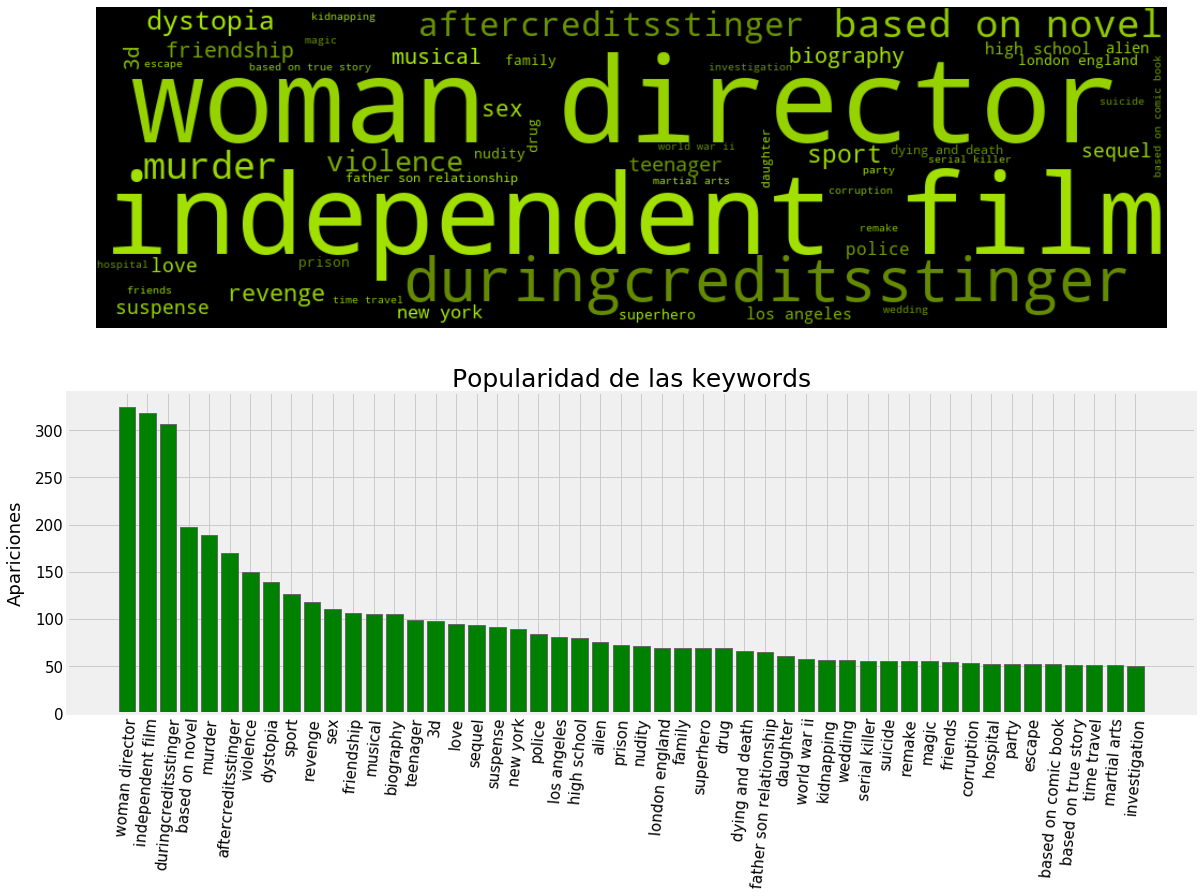
\includegraphics[height=10cm]{./contenido/imagenes/output_17_0.png}
\end{figure}
    { \hspace*{\fill} \\}
    
    \begin{center}\rule{0.5\linewidth}{\linethickness}\end{center}

\subsubsection{1.2 Factor de completitud: Valores
Faltantes}\label{factor-de-completitud-valores-faltantes}

El conjunto de datos consiste en 5043 películas o series que están
descritas mediante 28 variables. Como en todo análisis, habrá que trater
con los valores faltantes y, como un primer paso, se calcula la cantidad
de datos faltantes en cada variable:

    \begin{tcolorbox}[breakable, size=fbox, boxrule=1pt, pad at break*=1mm,colback=cellbackground, colframe=cellborder]
\prompt{In}{incolor}{12}{\hspace{4pt}}
\begin{Verbatim}[commandchars=\\\{\}]
\PY{n}{missing\PYZus{}df} \PY{o}{=} \PY{n}{df\PYZus{}initial}\PY{o}{.}\PY{n}{isnull}\PY{p}{(}\PY{p}{)}\PY{o}{.}\PY{n}{sum}\PY{p}{(}\PY{n}{axis}\PY{o}{=}\PY{l+m+mi}{0}\PY{p}{)}\PY{o}{.}\PY{n}{reset\PYZus{}index}\PY{p}{(}\PY{p}{)}
\PY{n}{missing\PYZus{}df}\PY{o}{.}\PY{n}{columns} \PY{o}{=} \PY{p}{[}\PY{l+s+s1}{\PYZsq{}}\PY{l+s+s1}{column\PYZus{}name}\PY{l+s+s1}{\PYZsq{}}\PY{p}{,} \PY{l+s+s1}{\PYZsq{}}\PY{l+s+s1}{missing\PYZus{}count}\PY{l+s+s1}{\PYZsq{}}\PY{p}{]}
\PY{n}{missing\PYZus{}df}\PY{p}{[}\PY{l+s+s1}{\PYZsq{}}\PY{l+s+s1}{filling\PYZus{}factor}\PY{l+s+s1}{\PYZsq{}}\PY{p}{]} \PY{o}{=} \PY{p}{(}\PY{n}{df\PYZus{}initial}\PY{o}{.}\PY{n}{shape}\PY{p}{[}\PY{l+m+mi}{0}\PY{p}{]} 
                                \PY{o}{\PYZhy{}} \PY{n}{missing\PYZus{}df}\PY{p}{[}\PY{l+s+s1}{\PYZsq{}}\PY{l+s+s1}{missing\PYZus{}count}\PY{l+s+s1}{\PYZsq{}}\PY{p}{]}\PY{p}{)} \PY{o}{/} \PY{n}{df\PYZus{}initial}\PY{o}{.}\PY{n}{shape}\PY{p}{[}\PY{l+m+mi}{0}\PY{p}{]} \PY{o}{*} \PY{l+m+mi}{100}
\PY{n}{missing\PYZus{}df}\PY{o}{.}\PY{n}{sort\PYZus{}values}\PY{p}{(}\PY{l+s+s1}{\PYZsq{}}\PY{l+s+s1}{filling\PYZus{}factor}\PY{l+s+s1}{\PYZsq{}}\PY{p}{)}\PY{o}{.}\PY{n}{reset\PYZus{}index}\PY{p}{(}\PY{n}{drop} \PY{o}{=} \PY{k+kc}{True}\PY{p}{)}
\end{Verbatim}
\end{tcolorbox}

            \begin{tcolorbox}[breakable, boxrule=.5pt, size=fbox, pad at break*=1mm, opacityfill=0]
\prompt{Out}{outcolor}{12}{\hspace{3.5pt}}
\begin{Verbatim}[commandchars=\\\{\}]
             column\_name  missing\_count  filling\_factor
0               homepage           3091       35.644389
1                tagline            844       82.427649
2                country            174       96.377264
3           actor\_3\_name             93       98.063710
4               language             86       98.209452
5           actor\_2\_name             63       98.688320
6           actor\_1\_name             53       98.896523
7          director\_name             30       99.375390
8               overview              3       99.937539
9               duration              2       99.958359
10            title\_year              1       99.979180
11          release\_date              1       99.979180
12       num\_voted\_users              0      100.000000
13          vote\_average              0      100.000000
14           movie\_title              0      100.000000
15                budget              0      100.000000
16      spoken\_languages              0      100.000000
17  production\_countries              0      100.000000
18  production\_companies              0      100.000000
19            popularity              0      100.000000
20        original\_title              0      100.000000
21         plot\_keywords              0      100.000000
22                    id              0      100.000000
23                genres              0      100.000000
24                status              0      100.000000
25                 gross              0      100.000000
\end{Verbatim}
\end{tcolorbox}
        
    Podemos ver que la integridad de los datos es bastante buena, ya que
únicamente 2 de las 28 variables tienen un factor de competitud menor
del 93\%.

    \begin{center}\rule{0.5\linewidth}{\linethickness}\end{center}

\subsubsection{~1.3 Películas por año}\label{peluxedculas-por-auxf1o}

    La variable \textbf{title\_year} indica cuándo se lanzó una película.
Para tener una visión global de la forma en la que las películas se
distribuyen según esta variable, las agrupamos por décadas:

    \begin{tcolorbox}[breakable, size=fbox, boxrule=1pt, pad at break*=1mm,colback=cellbackground, colframe=cellborder]
\prompt{In}{incolor}{13}{\hspace{4pt}}
\begin{Verbatim}[commandchars=\\\{\}]
\PY{c+c1}{\PYZsh{}Obtenemos la década de cada película}

\PY{n}{df\PYZus{}initial}\PY{p}{[}\PY{l+s+s1}{\PYZsq{}}\PY{l+s+s1}{decade}\PY{l+s+s1}{\PYZsq{}}\PY{p}{]} \PY{o}{=} \PY{n}{df\PYZus{}initial}\PY{p}{[}\PY{l+s+s1}{\PYZsq{}}\PY{l+s+s1}{title\PYZus{}year}\PY{l+s+s1}{\PYZsq{}}\PY{p}{]}\PY{o}{.}\PY{n}{apply}\PY{p}{(}\PY{k}{lambda} \PY{n}{x}\PY{p}{:}\PY{p}{(}\PY{p}{(}\PY{n}{x}\PY{o}{\PYZhy{}}\PY{l+m+mi}{1900}\PY{p}{)}\PY{o}{/}\PY{o}{/}\PY{l+m+mi}{10}\PY{p}{)}\PY{o}{*}\PY{l+m+mi}{10}\PY{p}{)}
\PY{k}{def} \PY{n+nf}{get\PYZus{}stats}\PY{p}{(}\PY{n}{gr}\PY{p}{)}\PY{p}{:}
    \PY{l+s+sd}{\PYZdq{}\PYZdq{}\PYZdq{}Devuelve las estadísticas de un DataFrame agrupado}
\PY{l+s+sd}{    }
\PY{l+s+sd}{    Arguments:}
\PY{l+s+sd}{        gr \PYZhy{}\PYZhy{} DataFrame agrupado}
\PY{l+s+sd}{    }
\PY{l+s+sd}{    Returns:}
\PY{l+s+sd}{        dict \PYZhy{}\PYZhy{} Diccionario que contiene las estadísticas principales de cada grupo}
\PY{l+s+sd}{    \PYZdq{}\PYZdq{}\PYZdq{}}
    \PY{k}{return} \PY{p}{\PYZob{}}\PY{l+s+s1}{\PYZsq{}}\PY{l+s+s1}{min}\PY{l+s+s1}{\PYZsq{}}\PY{p}{:}\PY{n}{gr}\PY{o}{.}\PY{n}{min}\PY{p}{(}\PY{p}{)}\PY{p}{,}\PY{l+s+s1}{\PYZsq{}}\PY{l+s+s1}{max}\PY{l+s+s1}{\PYZsq{}}\PY{p}{:}\PY{n}{gr}\PY{o}{.}\PY{n}{max}\PY{p}{(}\PY{p}{)}\PY{p}{,}\PY{l+s+s1}{\PYZsq{}}\PY{l+s+s1}{count}\PY{l+s+s1}{\PYZsq{}}\PY{p}{:} \PY{n}{gr}\PY{o}{.}\PY{n}{count}\PY{p}{(}\PY{p}{)}\PY{p}{,}\PY{l+s+s1}{\PYZsq{}}\PY{l+s+s1}{mean}\PY{l+s+s1}{\PYZsq{}}\PY{p}{:}\PY{n}{gr}\PY{o}{.}\PY{n}{mean}\PY{p}{(}\PY{p}{)}\PY{p}{\PYZcb{}}\PY{c+c1}{\PYZsh{}\PYZus{}\PYZus{}\PYZus{}\PYZus{}\PYZus{}\PYZus{}\PYZus{}\PYZus{}\PYZus{}\PYZus{}\PYZus{}\PYZus{}\PYZus{}\PYZus{}\PYZus{}\PYZus{}\PYZus{}\PYZus{}\PYZus{}\PYZus{}\PYZus{}\PYZus{}\PYZus{}\PYZus{}\PYZus{}\PYZus{}\PYZus{}\PYZus{}\PYZus{}\PYZus{}\PYZus{}\PYZus{}\PYZus{}\PYZus{}\PYZus{}\PYZus{}\PYZus{}\PYZus{}\PYZus{}\PYZus{}\PYZus{}\PYZus{}\PYZus{}\PYZus{}\PYZus{}\PYZus{}\PYZus{}\PYZus{}\PYZus{}\PYZus{}\PYZus{}\PYZus{}\PYZus{}\PYZus{}\PYZus{}\PYZus{}\PYZus{}\PYZus{}\PYZus{}\PYZus{}\PYZus{}\PYZus{}}
\PY{c+c1}{\PYZsh{} Creación de un DataFrame con información estadística de cada década}
\PY{n}{test} \PY{o}{=} \PY{n}{df\PYZus{}initial}\PY{p}{[}\PY{l+s+s1}{\PYZsq{}}\PY{l+s+s1}{title\PYZus{}year}\PY{l+s+s1}{\PYZsq{}}\PY{p}{]}\PY{o}{.}\PY{n}{groupby}\PY{p}{(}\PY{n}{df\PYZus{}initial}\PY{p}{[}\PY{l+s+s1}{\PYZsq{}}\PY{l+s+s1}{decade}\PY{l+s+s1}{\PYZsq{}}\PY{p}{]}\PY{p}{)}\PY{o}{.}\PY{n}{apply}\PY{p}{(}\PY{n}{get\PYZus{}stats}\PY{p}{)}\PY{o}{.}\PY{n}{unstack}\PY{p}{(}\PY{p}{)}
\end{Verbatim}
\end{tcolorbox}

    y representamos los resultados en un diagrama de sectores

    \begin{tcolorbox}[breakable, size=fbox, boxrule=1pt, pad at break*=1mm,colback=cellbackground, colframe=cellborder]
\prompt{In}{incolor}{14}{\hspace{4pt}}
\begin{Verbatim}[commandchars=\\\{\}]
\PY{n}{sns}\PY{o}{.}\PY{n}{set\PYZus{}context}\PY{p}{(}\PY{l+s+s2}{\PYZdq{}}\PY{l+s+s2}{poster}\PY{l+s+s2}{\PYZdq{}}\PY{p}{,} \PY{n}{font\PYZus{}scale}\PY{o}{=}\PY{l+m+mf}{0.85}\PY{p}{)}


\PY{k}{def} \PY{n+nf}{label}\PY{p}{(}\PY{n}{s}\PY{p}{)}\PY{p}{:}
    \PY{l+s+sd}{\PYZdq{}\PYZdq{}\PYZdq{}}
\PY{l+s+sd}{    Get de label from the decade. If XX Century\PYZhy{}\PYZgt{} last 2 digits.}
\PY{l+s+sd}{    Else \PYZhy{}\PYZgt{} complete year}
\PY{l+s+sd}{    \PYZdq{}\PYZdq{}\PYZdq{}}
    \PY{n}{val} \PY{o}{=} \PY{p}{(}\PY{l+m+mi}{1900} \PY{o}{+} \PY{n}{s}\PY{p}{,} \PY{n}{s}\PY{p}{)}\PY{p}{[}\PY{n}{s} \PY{o}{\PYZlt{}} \PY{l+m+mi}{100}\PY{p}{]}
    \PY{n}{chaine} \PY{o}{=} \PY{l+s+s1}{\PYZsq{}}\PY{l+s+s1}{\PYZsq{}} \PY{k}{if} \PY{n}{s} \PY{o}{\PYZlt{}} \PY{l+m+mi}{50} \PY{k}{else} \PY{l+s+s2}{\PYZdq{}}\PY{l+s+si}{\PYZob{}\PYZcb{}}\PY{l+s+s2}{\PYZsq{}}\PY{l+s+s2}{s}\PY{l+s+s2}{\PYZdq{}}\PY{o}{.}\PY{n}{format}\PY{p}{(}\PY{n+nb}{int}\PY{p}{(}\PY{n}{val}\PY{p}{)}\PY{p}{)}
    \PY{k}{return} \PY{n}{chaine}

\PY{n}{plt}\PY{o}{.}\PY{n}{rc}\PY{p}{(}\PY{l+s+s1}{\PYZsq{}}\PY{l+s+s1}{font}\PY{l+s+s1}{\PYZsq{}}\PY{p}{,} \PY{n}{weight}\PY{o}{=}\PY{l+s+s1}{\PYZsq{}}\PY{l+s+s1}{bold}\PY{l+s+s1}{\PYZsq{}}\PY{p}{)}
\PY{n}{f}\PY{p}{,} \PY{n}{ax} \PY{o}{=} \PY{n}{plt}\PY{o}{.}\PY{n}{subplots}\PY{p}{(}\PY{n}{figsize}\PY{o}{=}\PY{p}{(}\PY{l+m+mi}{11}\PY{p}{,} \PY{l+m+mi}{6}\PY{p}{)}\PY{p}{)}
\PY{n}{labels} \PY{o}{=} \PY{p}{[}\PY{n}{label}\PY{p}{(}\PY{n}{s}\PY{p}{)} \PY{k}{for} \PY{n}{s} \PY{o+ow}{in}  \PY{n}{test}\PY{o}{.}\PY{n}{index}\PY{p}{]}
\PY{n}{sizes}  \PY{o}{=} \PY{n}{test}\PY{p}{[}\PY{l+s+s1}{\PYZsq{}}\PY{l+s+s1}{count}\PY{l+s+s1}{\PYZsq{}}\PY{p}{]}\PY{o}{.}\PY{n}{values}
\PY{n}{explode} \PY{o}{=} \PY{p}{[}\PY{l+m+mf}{0.2} \PY{k}{if} \PY{n}{sizes}\PY{p}{[}\PY{n}{i}\PY{p}{]} \PY{o}{\PYZlt{}} \PY{l+m+mi}{100} \PY{k}{else} \PY{l+m+mf}{0.01} \PY{k}{for} \PY{n}{i} \PY{o+ow}{in} \PY{n+nb}{range}\PY{p}{(}\PY{l+m+mi}{11}\PY{p}{)}\PY{p}{]}
\PY{n}{ax}\PY{o}{.}\PY{n}{pie}\PY{p}{(}\PY{n}{sizes}\PY{p}{,} \PY{n}{explode} \PY{o}{=} \PY{n}{explode}\PY{p}{,} \PY{n}{labels}\PY{o}{=}\PY{n}{labels}\PY{p}{,}
       \PY{n}{autopct} \PY{o}{=} \PY{k}{lambda} \PY{n}{x}\PY{p}{:}\PY{l+s+s1}{\PYZsq{}}\PY{l+s+si}{\PYZob{}:1.0f\PYZcb{}}\PY{l+s+s1}{\PYZpc{}}\PY{l+s+s1}{\PYZsq{}}\PY{o}{.}\PY{n}{format}\PY{p}{(}\PY{n}{x}\PY{p}{)} \PY{k}{if} \PY{n}{x} \PY{o}{\PYZgt{}} \PY{l+m+mi}{1} \PY{k}{else} \PY{l+s+s1}{\PYZsq{}}\PY{l+s+s1}{\PYZsq{}}\PY{p}{,}
       \PY{n}{shadow}\PY{o}{=}\PY{k+kc}{False}\PY{p}{,} \PY{n}{startangle}\PY{o}{=}\PY{l+m+mi}{0}\PY{p}{)}
\PY{n}{ax}\PY{o}{.}\PY{n}{axis}\PY{p}{(}\PY{l+s+s1}{\PYZsq{}}\PY{l+s+s1}{equal}\PY{l+s+s1}{\PYZsq{}}\PY{p}{)}
\PY{n}{ax}\PY{o}{.}\PY{n}{set\PYZus{}title}\PY{p}{(}\PY{l+s+s1}{\PYZsq{}}\PY{l+s+si}{\PYZpc{} d}\PY{l+s+s1}{e películas por década}\PY{l+s+s1}{\PYZsq{}}\PY{p}{,} \PY{n}{fontsize}\PY{o}{=}\PY{l+m+mi}{16}\PY{p}{)}\PY{p}{;}
\PY{n}{df\PYZus{}initial}\PY{o}{.}\PY{n}{drop}\PY{p}{(}\PY{l+s+s1}{\PYZsq{}}\PY{l+s+s1}{decade}\PY{l+s+s1}{\PYZsq{}}\PY{p}{,} \PY{n}{axis}\PY{o}{=}\PY{l+m+mi}{1}\PY{p}{,} \PY{n}{inplace} \PY{o}{=} \PY{k+kc}{True}\PY{p}{)}
\end{Verbatim}
\end{tcolorbox}

\begin{figure}[h]
    \centering
    \captionsetup{width=10cm}
    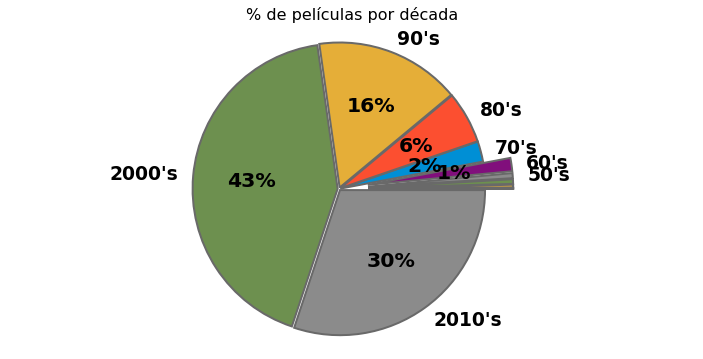
\includegraphics[width=10cm]{./contenido/imagenes/output_25_0.png}

\end{figure}

    { \hspace*{\fill} \\}
    
    \begin{center}\rule{0.5\linewidth}{\linethickness}\end{center}

\subsubsection{1.4 Géneros}\label{guxe9neros}

    La variable \textbf{genres} será importante en la creación del sistema
de recomendación, dado que describe el contenido de la película. Para
ver exactamente qué generos son los mas populares, se usa la misma
aproximación que con las keywords.

    \begin{tcolorbox}[breakable, size=fbox, boxrule=1pt, pad at break*=1mm,colback=cellbackground, colframe=cellborder]
\prompt{In}{incolor}{15}{\hspace{4pt}}
\begin{Verbatim}[commandchars=\\\{\}]
\PY{n}{genre\PYZus{}labels} \PY{o}{=} \PY{n+nb}{set}\PY{p}{(}\PY{p}{)}
\PY{k}{for} \PY{n}{s} \PY{o+ow}{in} \PY{n}{df\PYZus{}initial}\PY{p}{[}\PY{l+s+s1}{\PYZsq{}}\PY{l+s+s1}{genres}\PY{l+s+s1}{\PYZsq{}}\PY{p}{]}\PY{o}{.}\PY{n}{str}\PY{o}{.}\PY{n}{split}\PY{p}{(}\PY{l+s+s1}{\PYZsq{}}\PY{l+s+s1}{|}\PY{l+s+s1}{\PYZsq{}}\PY{p}{)}\PY{o}{.}\PY{n}{values}\PY{p}{:}
    \PY{n}{genre\PYZus{}labels} \PY{o}{=} \PY{n}{genre\PYZus{}labels}\PY{o}{.}\PY{n}{union}\PY{p}{(}\PY{n+nb}{set}\PY{p}{(}\PY{n}{s}\PY{p}{)}\PY{p}{)}
\end{Verbatim}
\end{tcolorbox}

    y cada genero aparece las siguientes veces:

    \begin{tcolorbox}[breakable, size=fbox, boxrule=1pt, pad at break*=1mm,colback=cellbackground, colframe=cellborder]
\prompt{In}{incolor}{16}{\hspace{4pt}}
\begin{Verbatim}[commandchars=\\\{\}]
\PY{n}{keyword\PYZus{}occurences}\PY{p}{,} \PY{n}{dum} \PY{o}{=} \PY{n}{count\PYZus{}word}\PY{p}{(}\PY{n}{df\PYZus{}initial}\PY{p}{,} \PY{l+s+s1}{\PYZsq{}}\PY{l+s+s1}{genres}\PY{l+s+s1}{\PYZsq{}}\PY{p}{,} \PY{n}{genre\PYZus{}labels}\PY{p}{)}
\PY{n}{keyword\PYZus{}occurences}\PY{p}{[}\PY{p}{:}\PY{l+m+mi}{5}\PY{p}{]}
\end{Verbatim}
\end{tcolorbox}

            \begin{tcolorbox}[breakable, boxrule=.5pt, size=fbox, pad at break*=1mm, opacityfill=0]
\prompt{Out}{outcolor}{16}{\hspace{3.5pt}}
\begin{Verbatim}[commandchars=\\\{\}]
[['Drama', 2297],
 ['Comedy', 1722],
 ['Thriller', 1274],
 ['Action', 1154],
 ['Romance', 894]]
\end{Verbatim}
\end{tcolorbox}
        
    \begin{tcolorbox}[breakable, size=fbox, boxrule=1pt, pad at break*=1mm,colback=cellbackground, colframe=cellborder]
\prompt{In}{incolor}{17}{\hspace{4pt}}
\begin{Verbatim}[commandchars=\\\{\}]
\PY{n}{keyword\PYZus{}occurences} \PY{o}{=} \PY{p}{[}\PY{n}{x} \PY{k}{for} \PY{n}{x} \PY{o+ow}{in} \PY{n}{keyword\PYZus{}occurences} \PY{k}{if} \PY{n}{x}\PY{p}{[}\PY{l+m+mi}{0}\PY{p}{]}\PY{p}{]}
\end{Verbatim}
\end{tcolorbox}

    Se muestra el resultado como una nube de palabras

    \begin{tcolorbox}[breakable, size=fbox, boxrule=1pt, pad at break*=1mm,colback=cellbackground, colframe=cellborder]
\prompt{In}{incolor}{18}{\hspace{4pt}}
\begin{Verbatim}[commandchars=\\\{\}]
\PY{n}{words} \PY{o}{=} \PY{n+nb}{dict}\PY{p}{(}\PY{p}{)}
\PY{n}{trunc\PYZus{}occurences} \PY{o}{=} \PY{n}{keyword\PYZus{}occurences}\PY{p}{[}\PY{l+m+mi}{0}\PY{p}{:}\PY{l+m+mi}{50}\PY{p}{]}
\PY{k}{for} \PY{n}{s} \PY{o+ow}{in} \PY{n}{trunc\PYZus{}occurences}\PY{p}{:}
    \PY{n}{words}\PY{p}{[}\PY{n}{s}\PY{p}{[}\PY{l+m+mi}{0}\PY{p}{]}\PY{p}{]} \PY{o}{=} \PY{n}{s}\PY{p}{[}\PY{l+m+mi}{1}\PY{p}{]}
\PY{n}{tone} \PY{o}{=} \PY{l+m+mi}{100} \PY{c+c1}{\PYZsh{} define the color of the words}
\PY{n}{f}\PY{p}{,} \PY{n}{ax} \PY{o}{=} \PY{n}{plt}\PY{o}{.}\PY{n}{subplots}\PY{p}{(}\PY{n}{figsize}\PY{o}{=}\PY{p}{(}\PY{l+m+mi}{14}\PY{p}{,} \PY{l+m+mi}{6}\PY{p}{)}\PY{p}{)}
\PY{n}{wordcloud} \PY{o}{=} \PY{n}{WordCloud}\PY{p}{(}\PY{n}{width}\PY{o}{=}\PY{l+m+mi}{550}\PY{p}{,}\PY{n}{height}\PY{o}{=}\PY{l+m+mi}{300}\PY{p}{,} \PY{n}{background\PYZus{}color}\PY{o}{=}\PY{l+s+s1}{\PYZsq{}}\PY{l+s+s1}{black}\PY{l+s+s1}{\PYZsq{}}\PY{p}{,} 
                      \PY{n}{max\PYZus{}words}\PY{o}{=}\PY{l+m+mi}{1628}\PY{p}{,}\PY{n}{relative\PYZus{}scaling}\PY{o}{=}\PY{l+m+mf}{0.7}\PY{p}{,}
                      \PY{n}{color\PYZus{}func} \PY{o}{=} \PY{n}{random\PYZus{}color\PYZus{}func}\PY{p}{,}
                      \PY{n}{normalize\PYZus{}plurals}\PY{o}{=}\PY{k+kc}{False}\PY{p}{)}
\PY{n}{wordcloud}\PY{o}{.}\PY{n}{generate\PYZus{}from\PYZus{}frequencies}\PY{p}{(}\PY{n}{words}\PY{p}{)}
\PY{n}{plt}\PY{o}{.}\PY{n}{imshow}\PY{p}{(}\PY{n}{wordcloud}\PY{p}{,} \PY{n}{interpolation}\PY{o}{=}\PY{l+s+s2}{\PYZdq{}}\PY{l+s+s2}{bilinear}\PY{l+s+s2}{\PYZdq{}}\PY{p}{)}
\PY{n}{plt}\PY{o}{.}\PY{n}{axis}\PY{p}{(}\PY{l+s+s1}{\PYZsq{}}\PY{l+s+s1}{off}\PY{l+s+s1}{\PYZsq{}}\PY{p}{)}
\PY{n}{plt}\PY{o}{.}\PY{n}{show}\PY{p}{(}\PY{p}{)}
\end{Verbatim}
\end{tcolorbox}
\begin{figure}[h]
    \centering
    \captionsetup{width=10cm}
    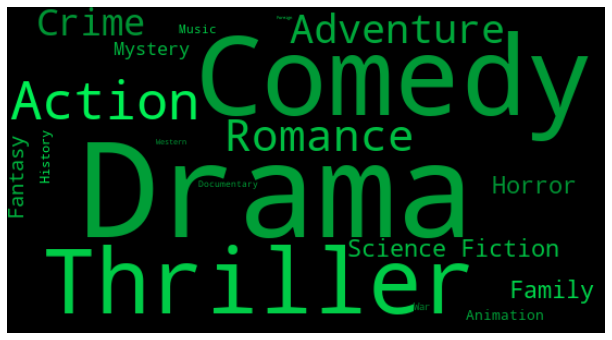
\includegraphics[width=10cm]{./contenido/imagenes/output_33_0.png}
\end{figure}

    { \hspace*{\fill} \\}
    
    \begin{center}\rule{0.5\linewidth}{\linethickness}\end{center}

\subsection{2. Limpieza}\label{limpieza}

\begin{center}\rule{0.5\linewidth}{\linethickness}\end{center}

\subsubsection{2.1 Entradas duplicadas}\label{entradas-duplicadas}

Hasta ahora, sólo mirabamos unas pocas variables e intentábamos
representar su contenido para tener una idea de su significado. Por
tanto, es ahora cuando empieza realmente la tarea de limpieza.

El primer paso consiste en buscar entradas duplicadas. Como un primer
paso, se comprueba si si las hay.

    \begin{tcolorbox}[breakable, size=fbox, boxrule=1pt, pad at break*=1mm,colback=cellbackground, colframe=cellborder]
\prompt{In}{incolor}{19}{\hspace{4pt}}
\begin{Verbatim}[commandchars=\\\{\}]
\PY{n}{doubled\PYZus{}entries} \PY{o}{=} \PY{n}{df\PYZus{}initial}\PY{p}{[}\PY{n}{df\PYZus{}initial}\PY{o}{.}\PY{n}{id}\PY{o}{.}\PY{n}{duplicated}\PY{p}{(}\PY{p}{)}\PY{p}{]}
\PY{n}{doubled\PYZus{}entries}\PY{o}{.}\PY{n}{shape}
\end{Verbatim}
\end{tcolorbox}

            \begin{tcolorbox}[breakable, boxrule=.5pt, size=fbox, pad at break*=1mm, opacityfill=0]
\prompt{Out}{outcolor}{19}{\hspace{3.5pt}}
\begin{Verbatim}[commandchars=\\\{\}]
(0, 26)
\end{Verbatim}
\end{tcolorbox}
        
    \begin{tcolorbox}[breakable, size=fbox, boxrule=1pt, pad at break*=1mm,colback=cellbackground, colframe=cellborder]
\prompt{In}{incolor}{20}{\hspace{4pt}}
\begin{Verbatim}[commandchars=\\\{\}]
\PY{n}{df\PYZus{}temp} \PY{o}{=} \PY{n}{df\PYZus{}initial}
\end{Verbatim}
\end{tcolorbox}

    Ahora examinamos lasfilas con entradas duplicadas teniendo en cuenta
únicamente las variables \textbf{movie\_title} y \textbf{title\_year},
and \textbf{director\_name}:

    \begin{tcolorbox}[breakable, size=fbox, boxrule=1pt, pad at break*=1mm,colback=cellbackground, colframe=cellborder]
\prompt{In}{incolor}{21}{\hspace{4pt}}
\begin{Verbatim}[commandchars=\\\{\}]
\PY{n}{list\PYZus{}var\PYZus{}duplicates} \PY{o}{=} \PY{p}{[}\PY{l+s+s1}{\PYZsq{}}\PY{l+s+s1}{movie\PYZus{}title}\PY{l+s+s1}{\PYZsq{}}\PY{p}{,} \PY{l+s+s1}{\PYZsq{}}\PY{l+s+s1}{title\PYZus{}year}\PY{l+s+s1}{\PYZsq{}}\PY{p}{,} \PY{l+s+s1}{\PYZsq{}}\PY{l+s+s1}{director\PYZus{}name}\PY{l+s+s1}{\PYZsq{}}\PY{p}{]}
\end{Verbatim}
\end{tcolorbox}

    Creamos una lista con las entradas con títulos idénticos:

    \begin{tcolorbox}[breakable, size=fbox, boxrule=1pt, pad at break*=1mm,colback=cellbackground, colframe=cellborder]
\prompt{In}{incolor}{22}{\hspace{4pt}}
\begin{Verbatim}[commandchars=\\\{\}]
\PY{n}{liste\PYZus{}duplicates} \PY{o}{=} \PY{n}{df\PYZus{}temp}\PY{p}{[}\PY{l+s+s1}{\PYZsq{}}\PY{l+s+s1}{movie\PYZus{}title}\PY{l+s+s1}{\PYZsq{}}\PY{p}{]}\PY{o}{.}\PY{n}{map}\PY{p}{(}\PY{n}{df\PYZus{}temp}\PY{p}{[}\PY{l+s+s1}{\PYZsq{}}\PY{l+s+s1}{movie\PYZus{}title}\PY{l+s+s1}{\PYZsq{}}\PY{p}{]}\PY{o}{.}\PY{n}{value\PYZus{}counts}\PY{p}{(}\PY{p}{)} \PY{o}{\PYZgt{}} \PY{l+m+mi}{1}\PY{p}{)}
\PY{n+nb}{print}\PY{p}{(}\PY{l+s+s2}{\PYZdq{}}\PY{l+s+s2}{Número de entradas duplicadas: }\PY{l+s+si}{\PYZob{}\PYZcb{}}\PY{l+s+s2}{\PYZdq{}}\PY{o}{.}\PY{n}{format}\PY{p}{(}
    \PY{n+nb}{len}\PY{p}{(}\PY{n}{df\PYZus{}temp}\PY{p}{[}\PY{n}{liste\PYZus{}duplicates}\PY{p}{]}\PY{p}{[}\PY{n}{list\PYZus{}var\PYZus{}duplicates}\PY{p}{]}\PY{p}{)}\PY{p}{)}\PY{p}{)}
\end{Verbatim}
\end{tcolorbox}

    \begin{Verbatim}[commandchars=\\\{\}]
Número de entradas duplicadas: 6
\end{Verbatim}

    y a continuación examinamos algunos casos. Dado que no hay demasiados
valores, es posible hacerlo a simple vista:

    \begin{tcolorbox}[breakable, size=fbox, boxrule=1pt, pad at break*=1mm,colback=cellbackground, colframe=cellborder]
\prompt{In}{incolor}{23}{\hspace{4pt}}
\begin{Verbatim}[commandchars=\\\{\}]
\PY{n}{df\PYZus{}temp}\PY{p}{[}\PY{n}{liste\PYZus{}duplicates}\PY{p}{]}\PY{p}{[}\PY{n}{list\PYZus{}var\PYZus{}duplicates}\PY{p}{]}\PY{o}{.}\PY{n}{sort\PYZus{}values}\PY{p}{(}\PY{l+s+s1}{\PYZsq{}}\PY{l+s+s1}{movie\PYZus{}title}\PY{l+s+s1}{\PYZsq{}}\PY{p}{)}
\end{Verbatim}
\end{tcolorbox}

            \begin{tcolorbox}[breakable, boxrule=.5pt, size=fbox, pad at break*=1mm, opacityfill=0]
\prompt{Out}{outcolor}{23}{\hspace{3.5pt}}
\begin{Verbatim}[commandchars=\\\{\}]
          movie\_title  title\_year        director\_name
1359           Batman      1989.0           Tim Burton
4267           Batman      1966.0  Leslie H. Martinson
3647  Out of the Blue      1980.0        Dennis Hopper
3693  Out of the Blue      2006.0       Robert Sarkies
972          The Host      2013.0        Andrew Niccol
2877         The Host      2006.0         Bong Joon-ho
\end{Verbatim}
\end{tcolorbox}
        
    Puede verse que estas películas son únicamente remakes.

    \begin{tcolorbox}[breakable, size=fbox, boxrule=1pt, pad at break*=1mm,colback=cellbackground, colframe=cellborder]
\prompt{In}{incolor}{24}{\hspace{4pt}}
\begin{Verbatim}[commandchars=\\\{\}]
\PY{n}{df\PYZus{}duplicate\PYZus{}cleaned} \PY{o}{=} \PY{n}{df\PYZus{}temp}
\end{Verbatim}
\end{tcolorbox}

    \begin{center}\rule{0.5\linewidth}{\linethickness}\end{center}

\subsubsection{2.2 Limpieza de keywords}\label{limpieza-de-keywords}

Las keywords tendrán un papel fundamental en el funcionamiento del
sistema. De hecho, las recomendaciones se basaran en la similaridad
entre películas. Para medir esas similaridades, se mirarán las películas
descritas por las mismas keywords. Por tanto, el contenido de la
variable \textbf{plot\_keywords} debe ser analizado, ya que será muy
utilizado.

    \begin{center}\rule{0.5\linewidth}{\linethickness}\end{center}

\paragraph{2.2.1 Agrupamiento por lexema}\label{agrupamiento-por-lexema}

Cogemos las keywords que aparecen en \textbf{plot\_keywords}. Esta lista
se limpia usando NLTK. Finalmente, veremos la ocurrencia de cada
keyword.

    \begin{tcolorbox}[breakable, size=fbox, boxrule=1pt, pad at break*=1mm,colback=cellbackground, colframe=cellborder]
\prompt{In}{incolor}{25}{\hspace{4pt}}
\begin{Verbatim}[commandchars=\\\{\}]
\PY{k}{def} \PY{n+nf}{keywords\PYZus{}inventory}\PY{p}{(}\PY{n}{dataframe}\PY{p}{,} \PY{n}{column} \PY{o}{=} \PY{l+s+s1}{\PYZsq{}}\PY{l+s+s1}{plot\PYZus{}keywords}\PY{l+s+s1}{\PYZsq{}}\PY{p}{)}\PY{p}{:}
    \PY{l+s+sd}{\PYZdq{}\PYZdq{}\PYZdq{}Devuelve un diccionario con las palabras que derivan de cada lexema}
\PY{l+s+sd}{    a partir de un DataFrame y la columna de la que se quiere extraer}
\PY{l+s+sd}{    }
\PY{l+s+sd}{    Arguments:}
\PY{l+s+sd}{        dataframe \PYZhy{}\PYZhy{} DataFrame del que obtener la información}
\PY{l+s+sd}{    }
\PY{l+s+sd}{    Keyword Arguments:}
\PY{l+s+sd}{        column \PYZob{}str\PYZcb{} \PYZhy{}\PYZhy{} Nombre de la columna (default: \PYZob{}\PYZsq{}plot\PYZus{}keywords\PYZsq{}\PYZcb{})}
\PY{l+s+sd}{    }
\PY{l+s+sd}{    Returns:}
\PY{l+s+sd}{        Lista con las keywords finales que aparecen}
\PY{l+s+sd}{        Diccionario con la relación lexema \PYZlt{}\PYZhy{}\PYZgt{} palabras}
\PY{l+s+sd}{        Diccionario con la palabra más corta derivada del lexema}
\PY{l+s+sd}{    \PYZdq{}\PYZdq{}\PYZdq{}}
    \PY{n}{PS} \PY{o}{=} \PY{n}{nltk}\PY{o}{.}\PY{n}{stem}\PY{o}{.}\PY{n}{PorterStemmer}\PY{p}{(}\PY{p}{)}
    \PY{n}{keywords\PYZus{}roots}  \PY{o}{=} \PY{n+nb}{dict}\PY{p}{(}\PY{p}{)}  \PY{c+c1}{\PYZsh{} recoger las palabras de cada lexema}
    \PY{n}{keywords\PYZus{}select} \PY{o}{=} \PY{n+nb}{dict}\PY{p}{(}\PY{p}{)}  \PY{c+c1}{\PYZsh{} asociacion: lexema \PYZlt{}\PYZhy{}\PYZgt{} keyword}
    \PY{n}{category\PYZus{}keys} \PY{o}{=} \PY{p}{[}\PY{p}{]}
    \PY{n}{icount} \PY{o}{=} \PY{l+m+mi}{0}
    \PY{k}{for} \PY{n}{s} \PY{o+ow}{in} \PY{n}{dataframe}\PY{p}{[}\PY{n}{column}\PY{p}{]}\PY{p}{:}
        \PY{k}{if} \PY{n}{pd}\PY{o}{.}\PY{n}{isnull}\PY{p}{(}\PY{n}{s}\PY{p}{)}\PY{p}{:} \PY{k}{continue}
        \PY{k}{for} \PY{n}{t} \PY{o+ow}{in} \PY{n}{s}\PY{o}{.}\PY{n}{split}\PY{p}{(}\PY{l+s+s1}{\PYZsq{}}\PY{l+s+s1}{|}\PY{l+s+s1}{\PYZsq{}}\PY{p}{)}\PY{p}{:}
            \PY{n}{t} \PY{o}{=} \PY{n}{t}\PY{o}{.}\PY{n}{lower}\PY{p}{(}\PY{p}{)} \PY{p}{;} \PY{n}{root} \PY{o}{=} \PY{n}{PS}\PY{o}{.}\PY{n}{stem}\PY{p}{(}\PY{n}{t}\PY{p}{)}
            \PY{c+c1}{\PYZsh{} Para cada lexema, un set con las palabras que lo usan}
            \PY{k}{if} \PY{n}{root} \PY{o+ow}{in} \PY{n}{keywords\PYZus{}roots}\PY{p}{:}                
                \PY{n}{keywords\PYZus{}roots}\PY{p}{[}\PY{n}{root}\PY{p}{]}\PY{o}{.}\PY{n}{add}\PY{p}{(}\PY{n}{t}\PY{p}{)}
            \PY{k}{else}\PY{p}{:}
                \PY{n}{keywords\PYZus{}roots}\PY{p}{[}\PY{n}{root}\PY{p}{]} \PY{o}{=} \PY{p}{\PYZob{}}\PY{n}{t}\PY{p}{\PYZcb{}}
    
    \PY{k}{for} \PY{n}{s} \PY{o+ow}{in} \PY{n}{keywords\PYZus{}roots}\PY{o}{.}\PY{n}{keys}\PY{p}{(}\PY{p}{)}\PY{p}{:}
        \PY{k}{if} \PY{n+nb}{len}\PY{p}{(}\PY{n}{keywords\PYZus{}roots}\PY{p}{[}\PY{n}{s}\PY{p}{]}\PY{p}{)} \PY{o}{\PYZgt{}} \PY{l+m+mi}{1}\PY{p}{:}  
            \PY{n}{min\PYZus{}length} \PY{o}{=} \PY{l+m+mi}{1000}
            \PY{k}{for} \PY{n}{k} \PY{o+ow}{in} \PY{n}{keywords\PYZus{}roots}\PY{p}{[}\PY{n}{s}\PY{p}{]}\PY{p}{:}
                \PY{k}{if} \PY{n+nb}{len}\PY{p}{(}\PY{n}{k}\PY{p}{)} \PY{o}{\PYZlt{}} \PY{n}{min\PYZus{}length}\PY{p}{:}
                    \PY{n}{key} \PY{o}{=} \PY{n}{k} \PY{p}{;} \PY{n}{min\PYZus{}length} \PY{o}{=} \PY{n+nb}{len}\PY{p}{(}\PY{n}{k}\PY{p}{)}            
            \PY{n}{category\PYZus{}keys}\PY{o}{.}\PY{n}{append}\PY{p}{(}\PY{n}{key}\PY{p}{)}
            \PY{n}{keywords\PYZus{}select}\PY{p}{[}\PY{n}{s}\PY{p}{]} \PY{o}{=} \PY{n}{key}
        \PY{k}{else}\PY{p}{:}
            \PY{n}{category\PYZus{}keys}\PY{o}{.}\PY{n}{append}\PY{p}{(}\PY{n+nb}{list}\PY{p}{(}\PY{n}{keywords\PYZus{}roots}\PY{p}{[}\PY{n}{s}\PY{p}{]}\PY{p}{)}\PY{p}{[}\PY{l+m+mi}{0}\PY{p}{]}\PY{p}{)}
            \PY{n}{keywords\PYZus{}select}\PY{p}{[}\PY{n}{s}\PY{p}{]} \PY{o}{=} \PY{n+nb}{list}\PY{p}{(}\PY{n}{keywords\PYZus{}roots}\PY{p}{[}\PY{n}{s}\PY{p}{]}\PY{p}{)}\PY{p}{[}\PY{l+m+mi}{0}\PY{p}{]}
                   
    \PY{n+nb}{print}\PY{p}{(}\PY{l+s+s2}{\PYZdq{}}\PY{l+s+s2}{Número de keywords en la variable: }\PY{l+s+s2}{\PYZsq{}}\PY{l+s+si}{\PYZob{}\PYZcb{}}\PY{l+s+s2}{\PYZsq{}}\PY{l+s+s2}{: }\PY{l+s+si}{\PYZob{}\PYZcb{}}\PY{l+s+s2}{\PYZdq{}}\PY{o}{.}\PY{n}{format}\PY{p}{(}\PY{n}{column}\PY{p}{,}\PY{n+nb}{len}\PY{p}{(}\PY{n}{category\PYZus{}keys}\PY{p}{)}\PY{p}{)}\PY{p}{)}
    \PY{k}{return} \PY{n}{category\PYZus{}keys}\PY{p}{,} \PY{n}{keywords\PYZus{}roots}\PY{p}{,} \PY{n}{keywords\PYZus{}select}
\end{Verbatim}
\end{tcolorbox}

    \begin{tcolorbox}[breakable, size=fbox, boxrule=1pt, pad at break*=1mm,colback=cellbackground, colframe=cellborder]
\prompt{In}{incolor}{26}{\hspace{4pt}}
\begin{Verbatim}[commandchars=\\\{\}]
\PY{n}{keywords}\PY{p}{,} \PY{n}{keywords\PYZus{}roots}\PY{p}{,} \PY{n}{keywords\PYZus{}select} \PY{o}{=} \PY{n}{keywords\PYZus{}inventory}\PY{p}{(}\PY{n}{df\PYZus{}duplicate\PYZus{}cleaned}\PY{p}{,}
                                                               \PY{n}{column} \PY{o}{=} \PY{l+s+s1}{\PYZsq{}}\PY{l+s+s1}{plot\PYZus{}keywords}\PY{l+s+s1}{\PYZsq{}}\PY{p}{)}
\end{Verbatim}
\end{tcolorbox}

    \begin{Verbatim}[commandchars=\\\{\}]
Número de keywords en la variable: 'plot\_keywords': 9474
\end{Verbatim}

    \begin{tcolorbox}[breakable, size=fbox, boxrule=1pt, pad at break*=1mm,colback=cellbackground, colframe=cellborder]
\prompt{In}{incolor}{27}{\hspace{4pt}}
\begin{Verbatim}[commandchars=\\\{\}]
\PY{c+c1}{\PYZsh{} Muestra de keywords que aparecen en formas similares}
\PY{c+c1}{\PYZsh{}\PYZhy{}\PYZhy{}\PYZhy{}\PYZhy{}\PYZhy{}\PYZhy{}\PYZhy{}\PYZhy{}\PYZhy{}\PYZhy{}\PYZhy{}\PYZhy{}\PYZhy{}\PYZhy{}\PYZhy{}\PYZhy{}\PYZhy{}\PYZhy{}\PYZhy{}\PYZhy{}\PYZhy{}\PYZhy{}\PYZhy{}\PYZhy{}\PYZhy{}\PYZhy{}\PYZhy{}\PYZhy{}\PYZhy{}\PYZhy{}\PYZhy{}\PYZhy{}\PYZhy{}\PYZhy{}\PYZhy{}\PYZhy{}\PYZhy{}\PYZhy{}\PYZhy{}\PYZhy{}\PYZhy{}\PYZhy{}\PYZhy{}\PYZhy{}\PYZhy{}\PYZhy{}\PYZhy{}\PYZhy{}\PYZhy{}\PYZhy{}\PYZhy{}\PYZhy{}\PYZhy{}\PYZhy{}\PYZhy{}\PYZhy{}\PYZhy{}\PYZhy{}\PYZhy{}\PYZhy{}}
\PY{n}{icount} \PY{o}{=} \PY{l+m+mi}{0}
\PY{k}{for} \PY{n}{s} \PY{o+ow}{in} \PY{n}{keywords\PYZus{}roots}\PY{o}{.}\PY{n}{keys}\PY{p}{(}\PY{p}{)}\PY{p}{:}
    \PY{k}{if} \PY{n+nb}{len}\PY{p}{(}\PY{n}{keywords\PYZus{}roots}\PY{p}{[}\PY{n}{s}\PY{p}{]}\PY{p}{)} \PY{o}{\PYZgt{}} \PY{l+m+mi}{1}\PY{p}{:} 
        \PY{n}{icount} \PY{o}{+}\PY{o}{=} \PY{l+m+mi}{1}
        \PY{k}{if} \PY{n}{icount} \PY{o}{\PYZlt{}} \PY{l+m+mi}{15}\PY{p}{:} \PY{n+nb}{print}\PY{p}{(}\PY{n}{icount}\PY{p}{,} \PY{n}{keywords\PYZus{}roots}\PY{p}{[}\PY{n}{s}\PY{p}{]}\PY{p}{,} \PY{n+nb}{len}\PY{p}{(}\PY{n}{keywords\PYZus{}roots}\PY{p}{[}\PY{n}{s}\PY{p}{]}\PY{p}{)}\PY{p}{)}
\end{Verbatim}
\end{tcolorbox}

    \begin{Verbatim}[commandchars=\\\{\}]
1 \{'alienation', 'alien'\} 2
2 \{'spying', 'spy'\} 2
3 \{'vigilante', 'vigilantism'\} 2
4 \{'terror', 'terrorism'\} 2
5 \{'flooding', 'flood'\} 2
6 \{'spiders', 'spider'\} 2
7 \{'horses', 'horse'\} 2
8 \{'music', 'musical'\} 2
9 \{'anime', 'animation', 'animal'\} 3
10 \{'compass', 'compassion'\} 2
11 \{'train', 'training'\} 2
12 \{'sail', 'sailing'\} 2
13 \{'time travel', 'time traveler'\} 2
14 \{'orcs', 'orc'\} 2
\end{Verbatim}

    \begin{tcolorbox}[breakable, size=fbox, boxrule=1pt, pad at break*=1mm,colback=cellbackground, colframe=cellborder]
\prompt{In}{incolor}{28}{\hspace{4pt}}
\begin{Verbatim}[commandchars=\\\{\}]
\PY{c+c1}{\PYZsh{} Reemplazo de keywords por su forma principal}
\PY{c+c1}{\PYZsh{}\PYZhy{}\PYZhy{}\PYZhy{}\PYZhy{}\PYZhy{}\PYZhy{}\PYZhy{}\PYZhy{}\PYZhy{}\PYZhy{}\PYZhy{}\PYZhy{}\PYZhy{}\PYZhy{}\PYZhy{}\PYZhy{}\PYZhy{}\PYZhy{}\PYZhy{}\PYZhy{}\PYZhy{}\PYZhy{}\PYZhy{}\PYZhy{}\PYZhy{}\PYZhy{}\PYZhy{}\PYZhy{}\PYZhy{}\PYZhy{}\PYZhy{}\PYZhy{}\PYZhy{}\PYZhy{}\PYZhy{}\PYZhy{}\PYZhy{}\PYZhy{}\PYZhy{}\PYZhy{}\PYZhy{}\PYZhy{}\PYZhy{}\PYZhy{}\PYZhy{}\PYZhy{}}
\PY{k}{def} \PY{n+nf}{df\PYZus{}keywords\PYZus{}replacement}\PY{p}{(}\PY{n}{df}\PY{p}{,} \PY{n}{replacement\PYZus{}dict}\PY{p}{,} \PY{n}{roots} \PY{o}{=} \PY{k+kc}{False}\PY{p}{,} \PY{n}{column} \PY{o}{=} \PY{l+s+s1}{\PYZsq{}}\PY{l+s+s1}{plot\PYZus{}keywords}\PY{l+s+s1}{\PYZsq{}}\PY{p}{)}\PY{p}{:}
    \PY{l+s+sd}{\PYZdq{}\PYZdq{}\PYZdq{}Reemplaza las palabras clave de una película por las formas básicas de las mismas.}

\PY{l+s+sd}{    Arguments:}
\PY{l+s+sd}{        df \PYZhy{}\PYZhy{} DataFrame que contiene la información de las películas}
\PY{l+s+sd}{        replacement\PYZus{}dict \PYZhy{}\PYZhy{} diccionarion]}

\PY{l+s+sd}{    Keyword Arguments:}
\PY{l+s+sd}{        roots \PYZob{}bool\PYZcb{} \PYZhy{}\PYZhy{} Controla si se obtienen las raices de las palabras de las}
\PY{l+s+sd}{        keywords (default: \PYZob{}False\PYZcb{})}
\PY{l+s+sd}{        column \PYZhy{}\PYZhy{} Columna en la que realizar la transformación}

\PY{l+s+sd}{    Returns:}
\PY{l+s+sd}{        df\PYZus{}new \PYZhy{}\PYZhy{} DataFrame con las sustituciones realizadas}
\PY{l+s+sd}{    \PYZdq{}\PYZdq{}\PYZdq{}}
    \PY{n}{PS} \PY{o}{=} \PY{n}{nltk}\PY{o}{.}\PY{n}{stem}\PY{o}{.}\PY{n}{PorterStemmer}\PY{p}{(}\PY{p}{)}
    \PY{n}{df\PYZus{}new} \PY{o}{=} \PY{n}{df}\PY{o}{.}\PY{n}{copy}\PY{p}{(}\PY{n}{deep} \PY{o}{=} \PY{k+kc}{True}\PY{p}{)}
    \PY{k}{for} \PY{n}{index}\PY{p}{,} \PY{n}{row} \PY{o+ow}{in} \PY{n}{df\PYZus{}new}\PY{o}{.}\PY{n}{iterrows}\PY{p}{(}\PY{p}{)}\PY{p}{:}
        \PY{n}{chain} \PY{o}{=} \PY{n}{row}\PY{p}{[}\PY{n}{column}\PY{p}{]}
        \PY{k}{if} \PY{n}{pd}\PY{o}{.}\PY{n}{isnull}\PY{p}{(}\PY{n}{chain}\PY{p}{)}\PY{p}{:} \PY{k}{continue}
        \PY{n}{new\PYZus{}list} \PY{o}{=} \PY{p}{[}\PY{p}{]}
        \PY{k}{for} \PY{n}{s} \PY{o+ow}{in} \PY{n}{chain}\PY{o}{.}\PY{n}{split}\PY{p}{(}\PY{l+s+s1}{\PYZsq{}}\PY{l+s+s1}{|}\PY{l+s+s1}{\PYZsq{}}\PY{p}{)}\PY{p}{:} 
            \PY{n}{key} \PY{o}{=} \PY{n}{PS}\PY{o}{.}\PY{n}{stem}\PY{p}{(}\PY{n}{s}\PY{p}{)} \PY{k}{if} \PY{n}{roots} \PY{k}{else} \PY{n}{s}
            \PY{k}{if} \PY{n}{key} \PY{o+ow}{in} \PY{n}{replacement\PYZus{}dict}\PY{o}{.}\PY{n}{keys}\PY{p}{(}\PY{p}{)}\PY{p}{:}
                \PY{n}{new\PYZus{}list}\PY{o}{.}\PY{n}{append}\PY{p}{(}\PY{n}{replacement\PYZus{}dict}\PY{p}{[}\PY{n}{key}\PY{p}{]}\PY{p}{)}
            \PY{k}{else}\PY{p}{:}
                \PY{n}{new\PYZus{}list}\PY{o}{.}\PY{n}{append}\PY{p}{(}\PY{n}{s}\PY{p}{)}       
        \PY{n}{df\PYZus{}new}\PY{o}{.}\PY{n}{set\PYZus{}value}\PY{p}{(}\PY{n}{index}\PY{p}{,} \PY{n}{column}\PY{p}{,} \PY{l+s+s1}{\PYZsq{}}\PY{l+s+s1}{|}\PY{l+s+s1}{\PYZsq{}}\PY{o}{.}\PY{n}{join}\PY{p}{(}\PY{n}{new\PYZus{}list}\PY{p}{)}\PY{p}{)} 
    \PY{k}{return} \PY{n}{df\PYZus{}new}
\end{Verbatim}
\end{tcolorbox}

    \begin{tcolorbox}[breakable, size=fbox, boxrule=1pt, pad at break*=1mm,colback=cellbackground, colframe=cellborder]
\prompt{In}{incolor}{29}{\hspace{4pt}}
\begin{Verbatim}[commandchars=\\\{\}]
\PY{c+c1}{\PYZsh{} Reemplazo de keywords por su forma principal}
\PY{c+c1}{\PYZsh{}\PYZhy{}\PYZhy{}\PYZhy{}\PYZhy{}\PYZhy{}\PYZhy{}\PYZhy{}\PYZhy{}\PYZhy{}\PYZhy{}\PYZhy{}\PYZhy{}\PYZhy{}\PYZhy{}\PYZhy{}\PYZhy{}\PYZhy{}\PYZhy{}\PYZhy{}\PYZhy{}\PYZhy{}\PYZhy{}\PYZhy{}\PYZhy{}\PYZhy{}\PYZhy{}\PYZhy{}\PYZhy{}\PYZhy{}\PYZhy{}\PYZhy{}\PYZhy{}\PYZhy{}\PYZhy{}\PYZhy{}\PYZhy{}\PYZhy{}\PYZhy{}\PYZhy{}\PYZhy{}\PYZhy{}\PYZhy{}\PYZhy{}\PYZhy{}\PYZhy{}\PYZhy{}\PYZhy{}\PYZhy{}\PYZhy{}}
\PY{n}{df\PYZus{}keywords\PYZus{}cleaned} \PY{o}{=} \PY{n}{df\PYZus{}keywords\PYZus{}replacement}\PY{p}{(}\PY{n}{df\PYZus{}duplicate\PYZus{}cleaned}\PY{p}{,} \PY{n}{keywords\PYZus{}select}\PY{p}{,}
                                               \PY{n}{roots} \PY{o}{=} \PY{k+kc}{True}\PY{p}{)}
\end{Verbatim}
\end{tcolorbox}

    \begin{tcolorbox}[breakable, size=fbox, boxrule=1pt, pad at break*=1mm,colback=cellbackground, colframe=cellborder]
\prompt{In}{incolor}{30}{\hspace{4pt}}
\begin{Verbatim}[commandchars=\\\{\}]
\PY{c+c1}{\PYZsh{} Conteo de la repetición de cada Keyword}
\PY{c+c1}{\PYZsh{}\PYZhy{}\PYZhy{}\PYZhy{}\PYZhy{}\PYZhy{}\PYZhy{}\PYZhy{}\PYZhy{}\PYZhy{}\PYZhy{}\PYZhy{}\PYZhy{}\PYZhy{}\PYZhy{}\PYZhy{}\PYZhy{}\PYZhy{}\PYZhy{}\PYZhy{}\PYZhy{}\PYZhy{}\PYZhy{}\PYZhy{}\PYZhy{}\PYZhy{}\PYZhy{}\PYZhy{}\PYZhy{}\PYZhy{}\PYZhy{}\PYZhy{}\PYZhy{}\PYZhy{}\PYZhy{}}
\PY{n}{keyword\PYZus{}occurences}\PY{p}{,} \PY{n}{keywords\PYZus{}count} \PY{o}{=} \PY{n}{count\PYZus{}word}\PY{p}{(}\PY{n}{df\PYZus{}keywords\PYZus{}cleaned}\PY{p}{,}\PY{l+s+s1}{\PYZsq{}}\PY{l+s+s1}{plot\PYZus{}keywords}\PY{l+s+s1}{\PYZsq{}}\PY{p}{,}\PY{n}{keywords}\PY{p}{)}
\PY{n}{keyword\PYZus{}occurences}\PY{p}{[}\PY{p}{:}\PY{l+m+mi}{5}\PY{p}{]}
\end{Verbatim}
\end{tcolorbox}

            \begin{tcolorbox}[breakable, boxrule=.5pt, size=fbox, pad at break*=1mm, opacityfill=0]
\prompt{Out}{outcolor}{30}{\hspace{3.5pt}}
\begin{Verbatim}[commandchars=\\\{\}]
[['', 412],
 ['woman director', 324],
 ['independent film', 318],
 ['duringcreditsstinger', 307],
 ['based on novel', 197]]
\end{Verbatim}
\end{tcolorbox}
        
    \begin{center}\rule{0.5\linewidth}{\linethickness}\end{center}

\paragraph{\texorpdfstring{2.2.2 Grupos de
\emph{sinónimos}}{2.2.2 Grupos de sinónimos}}\label{grupos-de-sinuxf3nimos}

Limpiamos la lista de keywords en dos pasos. En un primer paso, se
suprimer las keywords que aparecen menos de 5 veces y se reemplazan por
un sinónimo de mayor frecuencia. En un segundo paso, se suprimen las
keywords que aparecen en menos de 3 películas.

    \begin{tcolorbox}[breakable, size=fbox, boxrule=1pt, pad at break*=1mm,colback=cellbackground, colframe=cellborder]
\prompt{In}{incolor}{33}{\hspace{4pt}}
\begin{Verbatim}[commandchars=\\\{\}]
\PY{c+c1}{\PYZsh{} Obtener los sinónimos de la palabra \PYZsq{}keyword\PYZsq{}}
\PY{c+c1}{\PYZsh{}\PYZhy{}\PYZhy{}\PYZhy{}\PYZhy{}\PYZhy{}\PYZhy{}\PYZhy{}\PYZhy{}\PYZhy{}\PYZhy{}\PYZhy{}\PYZhy{}\PYZhy{}\PYZhy{}\PYZhy{}\PYZhy{}\PYZhy{}\PYZhy{}\PYZhy{}\PYZhy{}\PYZhy{}\PYZhy{}\PYZhy{}\PYZhy{}\PYZhy{}\PYZhy{}\PYZhy{}\PYZhy{}\PYZhy{}\PYZhy{}\PYZhy{}\PYZhy{}\PYZhy{}\PYZhy{}\PYZhy{}\PYZhy{}\PYZhy{}\PYZhy{}\PYZhy{}\PYZhy{}\PYZhy{}\PYZhy{}\PYZhy{}\PYZhy{}\PYZhy{}\PYZhy{}\PYZhy{}\PYZhy{}\PYZhy{}\PYZhy{}\PYZhy{}\PYZhy{}\PYZhy{}\PYZhy{}\PYZhy{}\PYZhy{}\PYZhy{}\PYZhy{}\PYZhy{}\PYZhy{}\PYZhy{}\PYZhy{}}
\PY{k}{def} \PY{n+nf}{get\PYZus{}synonyms}\PY{p}{(}\PY{n}{keyword}\PY{p}{)}\PY{p}{:}
    \PY{l+s+sd}{\PYZdq{}\PYZdq{}\PYZdq{}Se obtienen los sinónimos sustantivos de una palabra}

\PY{l+s+sd}{    Arguments:}
\PY{l+s+sd}{        keyword \PYZhy{}\PYZhy{} Palabra de la que obtener los sinónimos}


\PY{l+s+sd}{    Returns:}
\PY{l+s+sd}{        lemma \PYZhy{}\PYZhy{} Lista con los sinónimos}
\PY{l+s+sd}{    \PYZdq{}\PYZdq{}\PYZdq{}}

    \PY{n}{lemma} \PY{o}{=} \PY{n+nb}{set}\PY{p}{(}\PY{p}{)}
    \PY{k}{for} \PY{n}{ss} \PY{o+ow}{in} \PY{n}{wordnet}\PY{o}{.}\PY{n}{synsets}\PY{p}{(}\PY{n}{keyword}\PY{p}{)}\PY{p}{:}
        \PY{k}{for} \PY{n}{w} \PY{o+ow}{in} \PY{n}{ss}\PY{o}{.}\PY{n}{lemma\PYZus{}names}\PY{p}{(}\PY{p}{)}\PY{p}{:}
            \PY{c+c1}{\PYZsh{}\PYZus{}\PYZus{}\PYZus{}\PYZus{}\PYZus{}\PYZus{}\PYZus{}\PYZus{}\PYZus{}\PYZus{}\PYZus{}\PYZus{}\PYZus{}\PYZus{}\PYZus{}\PYZus{}\PYZus{}\PYZus{}\PYZus{}\PYZus{}\PYZus{}\PYZus{}\PYZus{}\PYZus{}\PYZus{}\PYZus{}\PYZus{}\PYZus{}\PYZus{}\PYZus{}\PYZus{}}
            \PY{c+c1}{\PYZsh{}  Obtenemos los sinónimos que son sustantivos}
            \PY{n}{index} \PY{o}{=} \PY{n}{ss}\PY{o}{.}\PY{n}{name}\PY{p}{(}\PY{p}{)}\PY{o}{.}\PY{n}{find}\PY{p}{(}\PY{l+s+s1}{\PYZsq{}}\PY{l+s+s1}{.}\PY{l+s+s1}{\PYZsq{}}\PY{p}{)}\PY{o}{+}\PY{l+m+mi}{1}
            \PY{k}{if} \PY{n}{ss}\PY{o}{.}\PY{n}{name}\PY{p}{(}\PY{p}{)}\PY{p}{[}\PY{n}{index}\PY{p}{]} \PY{o}{==} \PY{l+s+s1}{\PYZsq{}}\PY{l+s+s1}{n}\PY{l+s+s1}{\PYZsq{}}\PY{p}{:} \PY{n}{lemma}\PY{o}{.}\PY{n}{add}\PY{p}{(}\PY{n}{w}\PY{o}{.}\PY{n}{lower}\PY{p}{(}\PY{p}{)}\PY{o}{.}\PY{n}{replace}\PY{p}{(}\PY{l+s+s1}{\PYZsq{}}\PY{l+s+s1}{\PYZus{}}\PY{l+s+s1}{\PYZsq{}}\PY{p}{,}\PY{l+s+s1}{\PYZsq{}}\PY{l+s+s1}{ }\PY{l+s+s1}{\PYZsq{}}\PY{p}{)}\PY{p}{)}
    \PY{k}{return} \PY{n}{lemma}   
\end{Verbatim}
\end{tcolorbox}

    \begin{tcolorbox}[breakable, size=fbox, boxrule=1pt, pad at break*=1mm,colback=cellbackground, colframe=cellborder]
\prompt{In}{incolor}{34}{\hspace{4pt}}
\begin{Verbatim}[commandchars=\\\{\}]
\PY{c+c1}{\PYZsh{} Ejemplo de una lista de sinónimos dados por NLTK}
\PY{c+c1}{\PYZsh{}\PYZhy{}\PYZhy{}\PYZhy{}\PYZhy{}\PYZhy{}\PYZhy{}\PYZhy{}\PYZhy{}\PYZhy{}\PYZhy{}\PYZhy{}\PYZhy{}\PYZhy{}\PYZhy{}\PYZhy{}\PYZhy{}\PYZhy{}\PYZhy{}\PYZhy{}\PYZhy{}\PYZhy{}\PYZhy{}\PYZhy{}\PYZhy{}\PYZhy{}\PYZhy{}\PYZhy{}\PYZhy{}\PYZhy{}\PYZhy{}\PYZhy{}\PYZhy{}\PYZhy{}\PYZhy{}\PYZhy{}\PYZhy{}\PYZhy{}\PYZhy{}\PYZhy{}\PYZhy{}\PYZhy{}\PYZhy{}\PYZhy{}\PYZhy{}\PYZhy{}\PYZhy{}\PYZhy{}\PYZhy{}\PYZhy{}\PYZhy{}\PYZhy{}}
\PY{n}{keyword} \PY{o}{=} \PY{l+s+s1}{\PYZsq{}}\PY{l+s+s1}{alien}\PY{l+s+s1}{\PYZsq{}}
\PY{n}{lemma} \PY{o}{=} \PY{n}{get\PYZus{}synonyms}\PY{p}{(}\PY{n}{keyword}\PY{p}{)}
\PY{k}{for} \PY{n}{s} \PY{o+ow}{in} \PY{n}{lemma}\PY{p}{:}
    \PY{n+nb}{print}\PY{p}{(}\PY{l+s+s1}{\PYZsq{}}\PY{l+s+s1}{ }\PY{l+s+s1}{\PYZdq{}}\PY{l+s+si}{\PYZob{}:\PYZlt{}30\PYZcb{}}\PY{l+s+s1}{\PYZdq{}}\PY{l+s+s1}{ in keywords list \PYZhy{}\PYZgt{} }\PY{l+s+si}{\PYZob{}\PYZcb{}}\PY{l+s+s1}{ }\PY{l+s+si}{\PYZob{}\PYZcb{}}\PY{l+s+s1}{\PYZsq{}}\PY{o}{.}\PY{n}{format}\PY{p}{(}\PY{n}{s}\PY{p}{,} \PY{n}{s} \PY{o+ow}{in} \PY{n}{keywords}\PY{p}{,}
                                                \PY{n}{keywords\PYZus{}count}\PY{p}{[}\PY{n}{s}\PY{p}{]} \PY{k}{if} \PY{n}{s} \PY{o+ow}{in} \PY{n}{keywords} \PY{k}{else} \PY{l+m+mi}{0} \PY{p}{)}\PY{p}{)}
\end{Verbatim}
\end{tcolorbox}

    \begin{Verbatim}[commandchars=\\\{\}]
 "extraterrestrial              " in keywords list -> True 4
 "unknown                       " in keywords list -> False 0
 "alien                         " in keywords list -> True 80
 "stranger                      " in keywords list -> True 7
 "extraterrestrial being        " in keywords list -> False 0
 "foreigner                     " in keywords list -> False 0
 "noncitizen                    " in keywords list -> False 0
 "outlander                     " in keywords list -> False 0
\end{Verbatim}

    \begin{tcolorbox}[breakable, size=fbox, boxrule=1pt, pad at break*=1mm,colback=cellbackground, colframe=cellborder]
\prompt{In}{incolor}{35}{\hspace{4pt}}
\begin{Verbatim}[commandchars=\\\{\}]
\PY{c+c1}{\PYZsh{} Comprobar si \PYZsq{}word\PYZsq{} es una clave con más ocurrecncias que el umbral   }
\PY{c+c1}{\PYZsh{}\PYZhy{}\PYZhy{}\PYZhy{}\PYZhy{}\PYZhy{}\PYZhy{}\PYZhy{}\PYZhy{}\PYZhy{}\PYZhy{}\PYZhy{}\PYZhy{}\PYZhy{}\PYZhy{}\PYZhy{}\PYZhy{}\PYZhy{}\PYZhy{}\PYZhy{}\PYZhy{}\PYZhy{}\PYZhy{}\PYZhy{}\PYZhy{}\PYZhy{}\PYZhy{}\PYZhy{}\PYZhy{}\PYZhy{}\PYZhy{}\PYZhy{}\PYZhy{}\PYZhy{}\PYZhy{}\PYZhy{}\PYZhy{}\PYZhy{}\PYZhy{}\PYZhy{}\PYZhy{}\PYZhy{}\PYZhy{}\PYZhy{}\PYZhy{}\PYZhy{}\PYZhy{}\PYZhy{}\PYZhy{}\PYZhy{}\PYZhy{}\PYZhy{}\PYZhy{}\PYZhy{}\PYZhy{}\PYZhy{}\PYZhy{}\PYZhy{}\PYZhy{}\PYZhy{}\PYZhy{}\PYZhy{}\PYZhy{}\PYZhy{}\PYZhy{}\PYZhy{}\PYZhy{}\PYZhy{}\PYZhy{}\PYZhy{}\PYZhy{}\PYZhy{}\PYZhy{}\PYZhy{}\PYZhy{}\PYZhy{}\PYZhy{}\PYZhy{}\PYZhy{}\PYZhy{}\PYZhy{}\PYZhy{}\PYZhy{}}
\PY{k}{def} \PY{n+nf}{test\PYZus{}keyword}\PY{p}{(}\PY{n}{word}\PY{p}{,} \PY{n}{key\PYZus{}count}\PY{p}{,} \PY{n}{threshold}\PY{p}{)}\PY{p}{:}
    \PY{l+s+sd}{\PYZdq{}\PYZdq{}\PYZdq{}Devuelve si una palabra aparece un número mayor de veces que el umbral señalado}

\PY{l+s+sd}{    Arguments:}
\PY{l+s+sd}{        word \PYZhy{}\PYZhy{} Palabra a busvcar}
\PY{l+s+sd}{        key\PYZus{}count \PYZhy{}\PYZhy{} Diccionario con las apariciones de cada keyword}
\PY{l+s+sd}{        threshold \PYZhy{}\PYZhy{} Umbral}

\PY{l+s+sd}{    Returns:}
\PY{l+s+sd}{        bool \PYZhy{}\PYZhy{} True si aparece un número mayor de veces}
\PY{l+s+sd}{    \PYZdq{}\PYZdq{}\PYZdq{}}
    \PY{k}{return} \PY{p}{(}\PY{k+kc}{False} \PY{p}{,} \PY{k+kc}{True}\PY{p}{)}\PY{p}{[}\PY{n}{key\PYZus{}count}\PY{o}{.}\PY{n}{get}\PY{p}{(}\PY{n}{word}\PY{p}{,} \PY{l+m+mi}{0}\PY{p}{)} \PY{o}{\PYZgt{}}\PY{o}{=} \PY{n}{threshold}\PY{p}{]} 
\end{Verbatim}
\end{tcolorbox}

    \begin{tcolorbox}[breakable, size=fbox, boxrule=1pt, pad at break*=1mm,colback=cellbackground, colframe=cellborder]
\prompt{In}{incolor}{37}{\hspace{4pt}}
\begin{Verbatim}[commandchars=\\\{\}]
\PY{n}{keyword\PYZus{}occurences}\PY{o}{.}\PY{n}{sort}\PY{p}{(}\PY{n}{key} \PY{o}{=} \PY{k}{lambda} \PY{n}{x}\PY{p}{:}\PY{n}{x}\PY{p}{[}\PY{l+m+mi}{1}\PY{p}{]}\PY{p}{,} \PY{n}{reverse} \PY{o}{=} \PY{k+kc}{False}\PY{p}{)}
\PY{n}{key\PYZus{}count} \PY{o}{=} \PY{n+nb}{dict}\PY{p}{(}\PY{p}{)}
\PY{k}{for} \PY{n}{s} \PY{o+ow}{in} \PY{n}{keyword\PYZus{}occurences}\PY{p}{:}
    \PY{n}{key\PYZus{}count}\PY{p}{[}\PY{n}{s}\PY{p}{[}\PY{l+m+mi}{0}\PY{p}{]}\PY{p}{]} \PY{o}{=} \PY{n}{s}\PY{p}{[}\PY{l+m+mi}{1}\PY{p}{]}
\PY{c+c1}{\PYZsh{}\PYZus{}\PYZus{}\PYZus{}\PYZus{}\PYZus{}\PYZus{}\PYZus{}\PYZus{}\PYZus{}\PYZus{}\PYZus{}\PYZus{}\PYZus{}\PYZus{}\PYZus{}\PYZus{}\PYZus{}\PYZus{}\PYZus{}\PYZus{}\PYZus{}\PYZus{}\PYZus{}\PYZus{}\PYZus{}\PYZus{}\PYZus{}\PYZus{}\PYZus{}\PYZus{}\PYZus{}\PYZus{}\PYZus{}\PYZus{}\PYZus{}\PYZus{}\PYZus{}\PYZus{}\PYZus{}\PYZus{}\PYZus{}\PYZus{}\PYZus{}\PYZus{}\PYZus{}\PYZus{}\PYZus{}\PYZus{}\PYZus{}\PYZus{}\PYZus{}\PYZus{}\PYZus{}\PYZus{}\PYZus{}\PYZus{}\PYZus{}\PYZus{}\PYZus{}\PYZus{}\PYZus{}\PYZus{}\PYZus{}\PYZus{}\PYZus{}\PYZus{}\PYZus{}\PYZus{}\PYZus{}\PYZus{}\PYZus{}\PYZus{}\PYZus{}\PYZus{}}
\PY{c+c1}{\PYZsh{} Creación de un diccionario para reemplazar keywords por sinónimos de mayor frecuencia}
\PY{n}{remplacement\PYZus{}word} \PY{o}{=} \PY{n+nb}{dict}\PY{p}{(}\PY{p}{)}
\PY{n}{icount} \PY{o}{=} \PY{l+m+mi}{0}
\PY{k}{for} \PY{n}{index}\PY{p}{,} \PY{p}{[}\PY{n}{word}\PY{p}{,} \PY{n}{nb\PYZus{}apparitions}\PY{p}{]} \PY{o+ow}{in} \PY{n+nb}{enumerate}\PY{p}{(}\PY{n}{keyword\PYZus{}occurences}\PY{p}{)}\PY{p}{:}
    \PY{k}{if} \PY{n}{nb\PYZus{}apparitions} \PY{o}{\PYZgt{}} \PY{l+m+mi}{5}\PY{p}{:} \PY{k}{continue}  \PY{c+c1}{\PYZsh{} Sólo las keywords que aparecen menos de 5 veces}
    \PY{n}{lemma} \PY{o}{=} \PY{n}{get\PYZus{}synonyms}\PY{p}{(}\PY{n}{word}\PY{p}{)}
    \PY{k}{if} \PY{n+nb}{len}\PY{p}{(}\PY{n}{lemma}\PY{p}{)} \PY{o}{==} \PY{l+m+mi}{0}\PY{p}{:} \PY{k}{continue}     \PY{c+c1}{\PYZsh{}Caso de plurales}
    \PY{c+c1}{\PYZsh{}\PYZus{}\PYZus{}\PYZus{}\PYZus{}\PYZus{}\PYZus{}\PYZus{}\PYZus{}\PYZus{}\PYZus{}\PYZus{}\PYZus{}\PYZus{}\PYZus{}\PYZus{}\PYZus{}\PYZus{}\PYZus{}\PYZus{}\PYZus{}\PYZus{}\PYZus{}\PYZus{}\PYZus{}\PYZus{}\PYZus{}\PYZus{}\PYZus{}\PYZus{}\PYZus{}\PYZus{}\PYZus{}\PYZus{}\PYZus{}\PYZus{}\PYZus{}\PYZus{}\PYZus{}\PYZus{}\PYZus{}\PYZus{}\PYZus{}\PYZus{}\PYZus{}\PYZus{}\PYZus{}\PYZus{}\PYZus{}\PYZus{}\PYZus{}\PYZus{}\PYZus{}\PYZus{}\PYZus{}\PYZus{}\PYZus{}\PYZus{}\PYZus{}\PYZus{}\PYZus{}\PYZus{}\PYZus{}\PYZus{}\PYZus{}\PYZus{}}
    \PY{n}{word\PYZus{}list} \PY{o}{=} \PY{p}{[}\PY{p}{(}\PY{n}{s}\PY{p}{,} \PY{n}{key\PYZus{}count}\PY{p}{[}\PY{n}{s}\PY{p}{]}\PY{p}{)} \PY{k}{for} \PY{n}{s} \PY{o+ow}{in} \PY{n}{lemma} 
                  \PY{k}{if} \PY{n}{test\PYZus{}keyword}\PY{p}{(}\PY{n}{s}\PY{p}{,} \PY{n}{key\PYZus{}count}\PY{p}{,} \PY{n}{key\PYZus{}count}\PY{p}{[}\PY{n}{word}\PY{p}{]}\PY{p}{)}\PY{p}{]}
    \PY{n}{word\PYZus{}list}\PY{o}{.}\PY{n}{sort}\PY{p}{(}\PY{n}{key} \PY{o}{=} \PY{k}{lambda} \PY{n}{x}\PY{p}{:}\PY{p}{(}\PY{n}{x}\PY{p}{[}\PY{l+m+mi}{1}\PY{p}{]}\PY{p}{,}\PY{n}{x}\PY{p}{[}\PY{l+m+mi}{0}\PY{p}{]}\PY{p}{)}\PY{p}{,} \PY{n}{reverse} \PY{o}{=} \PY{k+kc}{True}\PY{p}{)}    
    \PY{k}{if} \PY{n+nb}{len}\PY{p}{(}\PY{n}{word\PYZus{}list}\PY{p}{)} \PY{o}{\PYZlt{}}\PY{o}{=} \PY{l+m+mi}{1}\PY{p}{:} \PY{k}{continue}       \PY{c+c1}{\PYZsh{} NO se reemplaza}
    \PY{k}{if} \PY{n}{word} \PY{o}{==} \PY{n}{word\PYZus{}list}\PY{p}{[}\PY{l+m+mi}{0}\PY{p}{]}\PY{p}{[}\PY{l+m+mi}{0}\PY{p}{]}\PY{p}{:} \PY{k}{continue}    \PY{c+c1}{\PYZsh{} Reemplazo por sí mismo}
    \PY{n}{icount} \PY{o}{+}\PY{o}{=} \PY{l+m+mi}{1}
    \PY{k}{if}  \PY{n}{icount} \PY{o}{\PYZlt{}} \PY{l+m+mi}{8}\PY{p}{:}
        \PY{n+nb}{print}\PY{p}{(}\PY{l+s+s1}{\PYZsq{}}\PY{l+s+si}{\PYZob{}:\PYZlt{}12\PYZcb{}}\PY{l+s+s1}{ \PYZhy{}\PYZgt{} }\PY{l+s+si}{\PYZob{}:\PYZlt{}12\PYZcb{}}\PY{l+s+s1}{ (init: }\PY{l+s+si}{\PYZob{}\PYZcb{}}\PY{l+s+s1}{)}\PY{l+s+s1}{\PYZsq{}}\PY{o}{.}\PY{n}{format}\PY{p}{(}\PY{n}{word}\PY{p}{,} \PY{n}{word\PYZus{}list}\PY{p}{[}\PY{l+m+mi}{0}\PY{p}{]}\PY{p}{[}\PY{l+m+mi}{0}\PY{p}{]}\PY{p}{,} \PY{n}{word\PYZus{}list}\PY{p}{)}\PY{p}{)}    
    \PY{n}{remplacement\PYZus{}word}\PY{p}{[}\PY{n}{word}\PY{p}{]} \PY{o}{=} \PY{n}{word\PYZus{}list}\PY{p}{[}\PY{l+m+mi}{0}\PY{p}{]}\PY{p}{[}\PY{l+m+mi}{0}\PY{p}{]}

\PY{n+nb}{print}\PY{p}{(}\PY{l+m+mi}{90}\PY{o}{*}\PY{l+s+s1}{\PYZsq{}}\PY{l+s+s1}{\PYZus{}}\PY{l+s+s1}{\PYZsq{}}\PY{o}{+}\PY{l+s+s1}{\PYZsq{}}\PY{l+s+se}{\PYZbs{}n}\PY{l+s+s1}{\PYZsq{}}\PY{o}{+}\PY{l+s+s1}{\PYZsq{}}\PY{l+s+s1}{The replacement concerns }\PY{l+s+si}{\PYZob{}\PYZcb{}}\PY{l+s+si}{\PYZpc{} o}\PY{l+s+s1}{f the keywords.}\PY{l+s+s1}{\PYZsq{}}
      \PY{o}{.}\PY{n}{format}\PY{p}{(}\PY{n+nb}{round}\PY{p}{(}\PY{n+nb}{len}\PY{p}{(}\PY{n}{remplacement\PYZus{}word}\PY{p}{)}\PY{o}{/}\PY{n+nb}{len}\PY{p}{(}\PY{n}{keywords}\PY{p}{)}\PY{o}{*}\PY{l+m+mi}{100}\PY{p}{,}\PY{l+m+mi}{2}\PY{p}{)}\PY{p}{)}\PY{p}{)}
\end{Verbatim}
\end{tcolorbox}

    \begin{Verbatim}[commandchars=\\\{\}]
narcism      -> narcissism   (init: [('narcissism', 1), ('narcism', 1)])
apparition   -> shadow       (init: [('shadow', 3), ('phantom', 3),
('apparition', 1)])
macao        -> macau        (init: [('macau', 1), ('macao', 1)])
regent       -> trustee      (init: [('trustee', 1), ('regent', 1)])
civilization -> culture      (init: [('culture', 2), ('civilization', 1)])
ark          -> ark of the covenant (init: [('ark of the covenant', 2), ('ark',
1)])
automaton    -> zombie       (init: [('zombie', 45), ('robot', 27),
('automaton', 1)])
\_\_\_\_\_\_\_\_\_\_\_\_\_\_\_\_\_\_\_\_\_\_\_\_\_\_\_\_\_\_\_\_\_\_\_\_\_\_\_\_\_\_\_\_\_\_\_\_\_\_\_\_\_\_\_\_\_\_\_\_\_\_\_\_\_\_\_\_\_\_\_\_\_\_\_\_\_\_\_\_
\_\_\_\_\_\_\_\_\_\_
The replacement concerns 5.95\% of the keywords.
\end{Verbatim}

    \begin{tcolorbox}[breakable, size=fbox, boxrule=1pt, pad at break*=1mm,colback=cellbackground, colframe=cellborder]
\prompt{In}{incolor}{38}{\hspace{4pt}}
\begin{Verbatim}[commandchars=\\\{\}]
\PY{c+c1}{\PYZsh{} 2 reemplazos sucesivos}
\PY{c+c1}{\PYZsh{}\PYZhy{}\PYZhy{}\PYZhy{}\PYZhy{}\PYZhy{}\PYZhy{}\PYZhy{}\PYZhy{}\PYZhy{}\PYZhy{}\PYZhy{}\PYZhy{}\PYZhy{}\PYZhy{}\PYZhy{}\PYZhy{}\PYZhy{}\PYZhy{}\PYZhy{}\PYZhy{}\PYZhy{}\PYZhy{}\PYZhy{}\PYZhy{}\PYZhy{}\PYZhy{}\PYZhy{}}
\PY{n+nb}{print}\PY{p}{(}\PY{l+s+s1}{\PYZsq{}}\PY{l+s+s1}{Keywords that appear both in keys and values:}\PY{l+s+s1}{\PYZsq{}}\PY{o}{.}\PY{n}{upper}\PY{p}{(}\PY{p}{)}\PY{o}{+}\PY{l+s+s1}{\PYZsq{}}\PY{l+s+se}{\PYZbs{}n}\PY{l+s+s1}{\PYZsq{}}\PY{o}{+}\PY{l+m+mi}{45}\PY{o}{*}\PY{l+s+s1}{\PYZsq{}}\PY{l+s+s1}{\PYZhy{}}\PY{l+s+s1}{\PYZsq{}}\PY{p}{)}
\PY{n}{icount} \PY{o}{=} \PY{l+m+mi}{0}
\PY{k}{for} \PY{n}{s} \PY{o+ow}{in} \PY{n}{remplacement\PYZus{}word}\PY{o}{.}\PY{n}{values}\PY{p}{(}\PY{p}{)}\PY{p}{:}
    \PY{k}{if} \PY{n}{s} \PY{o+ow}{in} \PY{n}{remplacement\PYZus{}word}\PY{o}{.}\PY{n}{keys}\PY{p}{(}\PY{p}{)}\PY{p}{:}
        \PY{n}{icount} \PY{o}{+}\PY{o}{=} \PY{l+m+mi}{1}
        \PY{k}{if} \PY{n}{icount} \PY{o}{\PYZlt{}} \PY{l+m+mi}{10}\PY{p}{:} \PY{n+nb}{print}\PY{p}{(}\PY{l+s+s1}{\PYZsq{}}\PY{l+s+si}{\PYZob{}:\PYZlt{}20\PYZcb{}}\PY{l+s+s1}{ \PYZhy{}\PYZgt{} }\PY{l+s+si}{\PYZob{}:\PYZlt{}20\PYZcb{}}\PY{l+s+s1}{\PYZsq{}}\PY{o}{.}\PY{n}{format}\PY{p}{(}\PY{n}{s}\PY{p}{,} \PY{n}{remplacement\PYZus{}word}\PY{p}{[}\PY{n}{s}\PY{p}{]}\PY{p}{)}\PY{p}{)}

\PY{k}{for} \PY{n}{key}\PY{p}{,} \PY{n}{value} \PY{o+ow}{in} \PY{n}{remplacement\PYZus{}word}\PY{o}{.}\PY{n}{items}\PY{p}{(}\PY{p}{)}\PY{p}{:}
    \PY{k}{if} \PY{n}{value} \PY{o+ow}{in} \PY{n}{remplacement\PYZus{}word}\PY{o}{.}\PY{n}{keys}\PY{p}{(}\PY{p}{)}\PY{p}{:}
        \PY{n}{remplacement\PYZus{}word}\PY{p}{[}\PY{n}{key}\PY{p}{]} \PY{o}{=} \PY{n}{remplacement\PYZus{}word}\PY{p}{[}\PY{n}{value}\PY{p}{]}                    
\end{Verbatim}
\end{tcolorbox}

    \begin{Verbatim}[commandchars=\\\{\}]
KEYWORDS THAT APPEAR BOTH IN KEYS AND VALUES:
---------------------------------------------
shadow               -> dark
failure              -> loser
leech                -> parasite
carnival             -> circus
pit                  -> hell
drawing              -> lottery
deal                 -> mountain
twist                -> crook
pest                 -> plague
\end{Verbatim}

    \begin{tcolorbox}[breakable, size=fbox, boxrule=1pt, pad at break*=1mm,colback=cellbackground, colframe=cellborder]
\prompt{In}{incolor}{41}{\hspace{4pt}}
\begin{Verbatim}[commandchars=\\\{\}]
\PY{c+c1}{\PYZsh{} Se reemplazan variaciones de una keyword por su keyword principal}
\PY{c+c1}{\PYZsh{}\PYZhy{}\PYZhy{}\PYZhy{}\PYZhy{}\PYZhy{}\PYZhy{}\PYZhy{}\PYZhy{}\PYZhy{}\PYZhy{}\PYZhy{}\PYZhy{}\PYZhy{}\PYZhy{}\PYZhy{}\PYZhy{}\PYZhy{}\PYZhy{}\PYZhy{}\PYZhy{}\PYZhy{}\PYZhy{}\PYZhy{}\PYZhy{}\PYZhy{}\PYZhy{}\PYZhy{}\PYZhy{}\PYZhy{}\PYZhy{}\PYZhy{}\PYZhy{}\PYZhy{}\PYZhy{}\PYZhy{}\PYZhy{}\PYZhy{}\PYZhy{}\PYZhy{}\PYZhy{}\PYZhy{}\PYZhy{}\PYZhy{}\PYZhy{}\PYZhy{}\PYZhy{}\PYZhy{}\PYZhy{}\PYZhy{}\PYZhy{}\PYZhy{}\PYZhy{}\PYZhy{}\PYZhy{}\PYZhy{}\PYZhy{}\PYZhy{}\PYZhy{}}
\PY{n}{df\PYZus{}keywords\PYZus{}synonyms} \PY{o}{=} \PYZbs{}
            \PY{n}{df\PYZus{}keywords\PYZus{}replacement}\PY{p}{(}\PY{n}{df\PYZus{}keywords\PYZus{}cleaned}\PY{p}{,} \PY{n}{remplacement\PYZus{}word}\PY{p}{,} \PY{n}{roots} \PY{o}{=} \PY{k+kc}{False}\PY{p}{)}   
\PY{n}{keywords}\PY{p}{,} \PY{n}{keywords\PYZus{}roots}\PY{p}{,} \PY{n}{keywords\PYZus{}select} \PY{o}{=} \PYZbs{}
            \PY{n}{keywords\PYZus{}inventory}\PY{p}{(}\PY{n}{df\PYZus{}keywords\PYZus{}synonyms}\PY{p}{,} \PY{n}{column} \PY{o}{=} \PY{l+s+s1}{\PYZsq{}}\PY{l+s+s1}{plot\PYZus{}keywords}\PY{l+s+s1}{\PYZsq{}}\PY{p}{)}
\end{Verbatim}
\end{tcolorbox}

    \begin{Verbatim}[commandchars=\\\{\}]
Número de keywords en la variable: 'plot\_keywords': 8911
\end{Verbatim}

    \begin{tcolorbox}[breakable, size=fbox, boxrule=1pt, pad at break*=1mm,colback=cellbackground, colframe=cellborder]
\prompt{In}{incolor}{42}{\hspace{4pt}}
\begin{Verbatim}[commandchars=\\\{\}]
\PY{c+c1}{\PYZsh{} Nuevo conteo de la ocurrencia de cada keyword}
\PY{c+c1}{\PYZsh{}\PYZhy{}\PYZhy{}\PYZhy{}\PYZhy{}\PYZhy{}\PYZhy{}\PYZhy{}\PYZhy{}\PYZhy{}\PYZhy{}\PYZhy{}\PYZhy{}\PYZhy{}\PYZhy{}\PYZhy{}\PYZhy{}\PYZhy{}\PYZhy{}\PYZhy{}\PYZhy{}\PYZhy{}\PYZhy{}\PYZhy{}\PYZhy{}\PYZhy{}\PYZhy{}\PYZhy{}\PYZhy{}\PYZhy{}\PYZhy{}\PYZhy{}\PYZhy{}\PYZhy{}\PYZhy{}\PYZhy{}\PYZhy{}\PYZhy{}}
\PY{n}{new\PYZus{}keyword\PYZus{}occurences}\PY{p}{,} \PY{n}{keywords\PYZus{}count} \PY{o}{=} \PY{n}{count\PYZus{}word}\PY{p}{(}\PY{n}{df\PYZus{}keywords\PYZus{}synonyms}\PY{p}{,}
                                                    \PY{l+s+s1}{\PYZsq{}}\PY{l+s+s1}{plot\PYZus{}keywords}\PY{l+s+s1}{\PYZsq{}}\PY{p}{,}\PY{n}{keywords}\PY{p}{)}
\PY{n}{new\PYZus{}keyword\PYZus{}occurences}\PY{p}{[}\PY{p}{:}\PY{l+m+mi}{5}\PY{p}{]}
\end{Verbatim}
\end{tcolorbox}

            \begin{tcolorbox}[breakable, boxrule=.5pt, size=fbox, pad at break*=1mm, opacityfill=0]
\prompt{Out}{outcolor}{42}{\hspace{3.5pt}}
\begin{Verbatim}[commandchars=\\\{\}]
[['', 412],
 ['woman director', 324],
 ['independent film', 318],
 ['duringcreditsstinger', 307],
 ['based on novel', 197]]
\end{Verbatim}
\end{tcolorbox}
        
    \begin{tcolorbox}[breakable, size=fbox, boxrule=1pt, pad at break*=1mm,colback=cellbackground, colframe=cellborder]
\prompt{In}{incolor}{45}{\hspace{4pt}}
\begin{Verbatim}[commandchars=\\\{\}]
\PY{c+c1}{\PYZsh{} Borrrado de keywords con baja frecuencia}
\PY{c+c1}{\PYZsh{}\PYZhy{}\PYZhy{}\PYZhy{}\PYZhy{}\PYZhy{}\PYZhy{}\PYZhy{}\PYZhy{}\PYZhy{}\PYZhy{}\PYZhy{}\PYZhy{}\PYZhy{}\PYZhy{}\PYZhy{}\PYZhy{}\PYZhy{}\PYZhy{}\PYZhy{}\PYZhy{}\PYZhy{}\PYZhy{}\PYZhy{}\PYZhy{}\PYZhy{}\PYZhy{}\PYZhy{}\PYZhy{}\PYZhy{}\PYZhy{}\PYZhy{}\PYZhy{}\PYZhy{}\PYZhy{}\PYZhy{}\PYZhy{}\PYZhy{}\PYZhy{}\PYZhy{}\PYZhy{}\PYZhy{}\PYZhy{}\PYZhy{}}
\PY{k}{def} \PY{n+nf}{replacement\PYZus{}df\PYZus{}low\PYZus{}frequency\PYZus{}keywords}\PY{p}{(}\PY{n}{df}\PY{p}{,} \PY{n}{keyword\PYZus{}occurences}\PY{p}{)}\PY{p}{:}
    \PY{l+s+sd}{\PYZdq{}\PYZdq{}\PYZdq{}Modifica las entradas del dataframe, quitando las keywords que aparecen menos de 3 veces.}

\PY{l+s+sd}{    Arguments:}
\PY{l+s+sd}{        df \PYZhy{}\PYZhy{} DataFrame de películas}
\PY{l+s+sd}{        keyword\PYZus{}occurences \PYZhy{}\PYZhy{} Diccionario que contiene la ocurrencia de cada keyword}

\PY{l+s+sd}{    Returns:}
\PY{l+s+sd}{        df \PYZhy{}\PYZhy{} DataFrame con las nuevas keywords}
\PY{l+s+sd}{    \PYZdq{}\PYZdq{}\PYZdq{}}
    \PY{n}{df\PYZus{}new} \PY{o}{=} \PY{n}{df}\PY{o}{.}\PY{n}{copy}\PY{p}{(}\PY{n}{deep} \PY{o}{=} \PY{k+kc}{True}\PY{p}{)}
    \PY{n}{key\PYZus{}count} \PY{o}{=} \PY{n+nb}{dict}\PY{p}{(}\PY{p}{)}
    \PY{k}{for} \PY{n}{s} \PY{o+ow}{in} \PY{n}{keyword\PYZus{}occurences}\PY{p}{:} 
        \PY{n}{key\PYZus{}count}\PY{p}{[}\PY{n}{s}\PY{p}{[}\PY{l+m+mi}{0}\PY{p}{]}\PY{p}{]} \PY{o}{=} \PY{n}{s}\PY{p}{[}\PY{l+m+mi}{1}\PY{p}{]}    
    \PY{k}{for} \PY{n}{index}\PY{p}{,} \PY{n}{row} \PY{o+ow}{in} \PY{n}{df\PYZus{}new}\PY{o}{.}\PY{n}{iterrows}\PY{p}{(}\PY{p}{)}\PY{p}{:}
        \PY{n}{chain} \PY{o}{=} \PY{n}{row}\PY{p}{[}\PY{l+s+s1}{\PYZsq{}}\PY{l+s+s1}{plot\PYZus{}keywords}\PY{l+s+s1}{\PYZsq{}}\PY{p}{]}
        \PY{k}{if} \PY{n}{pd}\PY{o}{.}\PY{n}{isnull}\PY{p}{(}\PY{n}{chain}\PY{p}{)}\PY{p}{:} \PY{k}{continue}
        \PY{n}{new\PYZus{}list} \PY{o}{=} \PY{p}{[}\PY{p}{]}
        \PY{k}{for} \PY{n}{s} \PY{o+ow}{in} \PY{n}{chain}\PY{o}{.}\PY{n}{split}\PY{p}{(}\PY{l+s+s1}{\PYZsq{}}\PY{l+s+s1}{|}\PY{l+s+s1}{\PYZsq{}}\PY{p}{)}\PY{p}{:} 
            \PY{k}{if} \PY{n}{key\PYZus{}count}\PY{o}{.}\PY{n}{get}\PY{p}{(}\PY{n}{s}\PY{p}{,} \PY{l+m+mi}{4}\PY{p}{)} \PY{o}{\PYZgt{}} \PY{l+m+mi}{3}\PY{p}{:} \PY{n}{new\PYZus{}list}\PY{o}{.}\PY{n}{append}\PY{p}{(}\PY{n}{s}\PY{p}{)}
        \PY{n}{df\PYZus{}new}\PY{o}{.}\PY{n}{set\PYZus{}value}\PY{p}{(}\PY{n}{index}\PY{p}{,} \PY{l+s+s1}{\PYZsq{}}\PY{l+s+s1}{plot\PYZus{}keywords}\PY{l+s+s1}{\PYZsq{}}\PY{p}{,} \PY{l+s+s1}{\PYZsq{}}\PY{l+s+s1}{|}\PY{l+s+s1}{\PYZsq{}}\PY{o}{.}\PY{n}{join}\PY{p}{(}\PY{n}{new\PYZus{}list}\PY{p}{)}\PY{p}{)}
    \PY{k}{return} \PY{n}{df\PYZus{}new}  
\end{Verbatim}
\end{tcolorbox}

    \begin{tcolorbox}[breakable, size=fbox, boxrule=1pt, pad at break*=1mm,colback=cellbackground, colframe=cellborder]
\prompt{In}{incolor}{46}{\hspace{4pt}}
\begin{Verbatim}[commandchars=\\\{\}]
\PY{c+c1}{\PYZsh{} Creation of a dataframe where keywords of low frequencies are suppressed}
\PY{c+c1}{\PYZsh{}\PYZhy{}\PYZhy{}\PYZhy{}\PYZhy{}\PYZhy{}\PYZhy{}\PYZhy{}\PYZhy{}\PYZhy{}\PYZhy{}\PYZhy{}\PYZhy{}\PYZhy{}\PYZhy{}\PYZhy{}\PYZhy{}\PYZhy{}\PYZhy{}\PYZhy{}\PYZhy{}\PYZhy{}\PYZhy{}\PYZhy{}\PYZhy{}\PYZhy{}\PYZhy{}\PYZhy{}\PYZhy{}\PYZhy{}\PYZhy{}\PYZhy{}\PYZhy{}\PYZhy{}\PYZhy{}\PYZhy{}\PYZhy{}\PYZhy{}\PYZhy{}\PYZhy{}\PYZhy{}\PYZhy{}\PYZhy{}\PYZhy{}\PYZhy{}\PYZhy{}\PYZhy{}\PYZhy{}\PYZhy{}\PYZhy{}\PYZhy{}\PYZhy{}\PYZhy{}\PYZhy{}\PYZhy{}\PYZhy{}\PYZhy{}\PYZhy{}\PYZhy{}\PYZhy{}\PYZhy{}\PYZhy{}\PYZhy{}\PYZhy{}\PYZhy{}\PYZhy{}\PYZhy{}\PYZhy{}\PYZhy{}\PYZhy{}\PYZhy{}\PYZhy{}\PYZhy{}\PYZhy{}}
\PY{n}{df\PYZus{}keywords\PYZus{}occurence} \PY{o}{=} \PYZbs{}
    \PY{n}{replacement\PYZus{}df\PYZus{}low\PYZus{}frequency\PYZus{}keywords}\PY{p}{(}\PY{n}{df\PYZus{}keywords\PYZus{}synonyms}\PY{p}{,} \PY{n}{new\PYZus{}keyword\PYZus{}occurences}\PY{p}{)}
\PY{n}{keywords}\PY{p}{,} \PY{n}{keywords\PYZus{}roots}\PY{p}{,} \PY{n}{keywords\PYZus{}select} \PY{o}{=} \PYZbs{}
    \PY{n}{keywords\PYZus{}inventory}\PY{p}{(}\PY{n}{df\PYZus{}keywords\PYZus{}occurence}\PY{p}{,} \PY{n}{column} \PY{o}{=} \PY{l+s+s1}{\PYZsq{}}\PY{l+s+s1}{plot\PYZus{}keywords}\PY{l+s+s1}{\PYZsq{}}\PY{p}{)}    
\end{Verbatim}
\end{tcolorbox}

    \begin{Verbatim}[commandchars=\\\{\}]
Número de keywords en la variable: 'plot\_keywords': 2121
\end{Verbatim}

    \begin{tcolorbox}[breakable, size=fbox, boxrule=1pt, pad at break*=1mm,colback=cellbackground, colframe=cellborder]
\prompt{In}{incolor}{47}{\hspace{4pt}}
\begin{Verbatim}[commandchars=\\\{\}]
\PY{c+c1}{\PYZsh{} Nuevo conteo de ocurrencia}
\PY{c+c1}{\PYZsh{}\PYZhy{}\PYZhy{}\PYZhy{}\PYZhy{}\PYZhy{}\PYZhy{}\PYZhy{}\PYZhy{}\PYZhy{}\PYZhy{}\PYZhy{}\PYZhy{}\PYZhy{}\PYZhy{}\PYZhy{}\PYZhy{}\PYZhy{}\PYZhy{}\PYZhy{}}
\PY{n}{new\PYZus{}keyword\PYZus{}occurences}\PY{p}{,} \PY{n}{keywords\PYZus{}count} \PY{o}{=} \PY{n}{count\PYZus{}word}\PY{p}{(}\PY{n}{df\PYZus{}keywords\PYZus{}occurence}\PY{p}{,}
                                                    \PY{l+s+s1}{\PYZsq{}}\PY{l+s+s1}{plot\PYZus{}keywords}\PY{l+s+s1}{\PYZsq{}}\PY{p}{,}\PY{n}{keywords}\PY{p}{)}
\PY{n}{new\PYZus{}keyword\PYZus{}occurences}\PY{p}{[}\PY{p}{:}\PY{l+m+mi}{5}\PY{p}{]}
\end{Verbatim}
\end{tcolorbox}

            \begin{tcolorbox}[breakable, boxrule=.5pt, size=fbox, pad at break*=1mm, opacityfill=0]
\prompt{Out}{outcolor}{47}{\hspace{3.5pt}}
\begin{Verbatim}[commandchars=\\\{\}]
[['', 508],
 ['woman director', 324],
 ['independent film', 318],
 ['duringcreditsstinger', 307],
 ['based on novel', 197]]
\end{Verbatim}
\end{tcolorbox}
        
    \begin{tcolorbox}[breakable, size=fbox, boxrule=1pt, pad at break*=1mm,colback=cellbackground, colframe=cellborder]
\prompt{In}{incolor}{48}{\hspace{4pt}}
\begin{Verbatim}[commandchars=\\\{\}]
\PY{c+c1}{\PYZsh{} Gráfico de ocurrencia de las keyword}
\PY{c+c1}{\PYZsh{}\PYZhy{}\PYZhy{}\PYZhy{}\PYZhy{}\PYZhy{}\PYZhy{}\PYZhy{}\PYZhy{}\PYZhy{}\PYZhy{}\PYZhy{}\PYZhy{}\PYZhy{}\PYZhy{}\PYZhy{}\PYZhy{}\PYZhy{}\PYZhy{}\PYZhy{}\PYZhy{}\PYZhy{}\PYZhy{}\PYZhy{}\PYZhy{}\PYZhy{}\PYZhy{}\PYZhy{}\PYZhy{}}
\PY{n}{font} \PY{o}{=} \PY{p}{\PYZob{}}\PY{l+s+s1}{\PYZsq{}}\PY{l+s+s1}{family}\PY{l+s+s1}{\PYZsq{}} \PY{p}{:} \PY{l+s+s1}{\PYZsq{}}\PY{l+s+s1}{fantasy}\PY{l+s+s1}{\PYZsq{}}\PY{p}{,} \PY{l+s+s1}{\PYZsq{}}\PY{l+s+s1}{weight}\PY{l+s+s1}{\PYZsq{}} \PY{p}{:} \PY{l+s+s1}{\PYZsq{}}\PY{l+s+s1}{normal}\PY{l+s+s1}{\PYZsq{}}\PY{p}{,} \PY{l+s+s1}{\PYZsq{}}\PY{l+s+s1}{size}\PY{l+s+s1}{\PYZsq{}}   \PY{p}{:} \PY{l+m+mi}{15}\PY{p}{\PYZcb{}}
\PY{n}{mpl}\PY{o}{.}\PY{n}{rc}\PY{p}{(}\PY{l+s+s1}{\PYZsq{}}\PY{l+s+s1}{font}\PY{l+s+s1}{\PYZsq{}}\PY{p}{,} \PY{o}{*}\PY{o}{*}\PY{n}{font}\PY{p}{)}

\PY{n}{keyword\PYZus{}occurences}\PY{o}{.}\PY{n}{sort}\PY{p}{(}\PY{n}{key} \PY{o}{=} \PY{k}{lambda} \PY{n}{x}\PY{p}{:}\PY{n}{x}\PY{p}{[}\PY{l+m+mi}{1}\PY{p}{]}\PY{p}{,} \PY{n}{reverse} \PY{o}{=} \PY{k+kc}{True}\PY{p}{)}

\PY{n}{y\PYZus{}axis} \PY{o}{=} \PY{p}{[}\PY{n}{i}\PY{p}{[}\PY{l+m+mi}{1}\PY{p}{]} \PY{k}{for} \PY{n}{i} \PY{o+ow}{in} \PY{n}{keyword\PYZus{}occurences}\PY{p}{]}
\PY{n}{x\PYZus{}axis} \PY{o}{=} \PY{p}{[}\PY{n}{k} \PY{k}{for} \PY{n}{k}\PY{p}{,}\PY{n}{i} \PY{o+ow}{in} \PY{n+nb}{enumerate}\PY{p}{(}\PY{n}{keyword\PYZus{}occurences}\PY{p}{)}\PY{p}{]}

\PY{n}{new\PYZus{}y\PYZus{}axis} \PY{o}{=} \PY{p}{[}\PY{n}{i}\PY{p}{[}\PY{l+m+mi}{1}\PY{p}{]} \PY{k}{for} \PY{n}{i} \PY{o+ow}{in} \PY{n}{new\PYZus{}keyword\PYZus{}occurences}\PY{p}{]}
\PY{n}{new\PYZus{}x\PYZus{}axis} \PY{o}{=} \PY{p}{[}\PY{n}{k} \PY{k}{for} \PY{n}{k}\PY{p}{,}\PY{n}{i} \PY{o+ow}{in} \PY{n+nb}{enumerate}\PY{p}{(}\PY{n}{new\PYZus{}keyword\PYZus{}occurences}\PY{p}{)}\PY{p}{]}

\PY{n}{f}\PY{p}{,} \PY{n}{ax} \PY{o}{=} \PY{n}{plt}\PY{o}{.}\PY{n}{subplots}\PY{p}{(}\PY{n}{figsize}\PY{o}{=}\PY{p}{(}\PY{l+m+mi}{9}\PY{p}{,} \PY{l+m+mi}{5}\PY{p}{)}\PY{p}{)}
\PY{n}{ax}\PY{o}{.}\PY{n}{plot}\PY{p}{(}\PY{n}{x\PYZus{}axis}\PY{p}{,} \PY{n}{y\PYZus{}axis}\PY{p}{,} \PY{l+s+s1}{\PYZsq{}}\PY{l+s+s1}{r\PYZhy{}}\PY{l+s+s1}{\PYZsq{}}\PY{p}{,} \PY{n}{label}\PY{o}{=}\PY{l+s+s1}{\PYZsq{}}\PY{l+s+s1}{before cleaning}\PY{l+s+s1}{\PYZsq{}}\PY{p}{)}
\PY{n}{ax}\PY{o}{.}\PY{n}{plot}\PY{p}{(}\PY{n}{new\PYZus{}x\PYZus{}axis}\PY{p}{,} \PY{n}{new\PYZus{}y\PYZus{}axis}\PY{p}{,} \PY{l+s+s1}{\PYZsq{}}\PY{l+s+s1}{b\PYZhy{}}\PY{l+s+s1}{\PYZsq{}}\PY{p}{,} \PY{n}{label}\PY{o}{=}\PY{l+s+s1}{\PYZsq{}}\PY{l+s+s1}{after cleaning}\PY{l+s+s1}{\PYZsq{}}\PY{p}{)}

\PY{c+c1}{\PYZsh{} Now add the legend with some customizations.}
\PY{n}{legend} \PY{o}{=} \PY{n}{ax}\PY{o}{.}\PY{n}{legend}\PY{p}{(}\PY{n}{loc}\PY{o}{=}\PY{l+s+s1}{\PYZsq{}}\PY{l+s+s1}{upper right}\PY{l+s+s1}{\PYZsq{}}\PY{p}{,} \PY{n}{shadow}\PY{o}{=}\PY{k+kc}{True}\PY{p}{)}
\PY{n}{frame} \PY{o}{=} \PY{n}{legend}\PY{o}{.}\PY{n}{get\PYZus{}frame}\PY{p}{(}\PY{p}{)}
\PY{n}{frame}\PY{o}{.}\PY{n}{set\PYZus{}facecolor}\PY{p}{(}\PY{l+s+s1}{\PYZsq{}}\PY{l+s+s1}{0.90}\PY{l+s+s1}{\PYZsq{}}\PY{p}{)}
\PY{k}{for} \PY{n}{label} \PY{o+ow}{in} \PY{n}{legend}\PY{o}{.}\PY{n}{get\PYZus{}texts}\PY{p}{(}\PY{p}{)}\PY{p}{:}
    \PY{n}{label}\PY{o}{.}\PY{n}{set\PYZus{}fontsize}\PY{p}{(}\PY{l+s+s1}{\PYZsq{}}\PY{l+s+s1}{medium}\PY{l+s+s1}{\PYZsq{}}\PY{p}{)}
            
\PY{n}{plt}\PY{o}{.}\PY{n}{ylim}\PY{p}{(}\PY{p}{(}\PY{l+m+mi}{0}\PY{p}{,}\PY{l+m+mi}{25}\PY{p}{)}\PY{p}{)}
\PY{n}{plt}\PY{o}{.}\PY{n}{axhline}\PY{p}{(}\PY{n}{y}\PY{o}{=}\PY{l+m+mf}{3.5}\PY{p}{,} \PY{n}{linewidth}\PY{o}{=}\PY{l+m+mi}{2}\PY{p}{,} \PY{n}{color} \PY{o}{=} \PY{l+s+s1}{\PYZsq{}}\PY{l+s+s1}{k}\PY{l+s+s1}{\PYZsq{}}\PY{p}{)}
\PY{n}{plt}\PY{o}{.}\PY{n}{xlabel}\PY{p}{(}\PY{l+s+s2}{\PYZdq{}}\PY{l+s+s2}{keywords index}\PY{l+s+s2}{\PYZdq{}}\PY{p}{,} \PY{n}{family}\PY{o}{=}\PY{l+s+s1}{\PYZsq{}}\PY{l+s+s1}{fantasy}\PY{l+s+s1}{\PYZsq{}}\PY{p}{,} \PY{n}{fontsize} \PY{o}{=} \PY{l+m+mi}{15}\PY{p}{)}
\PY{n}{plt}\PY{o}{.}\PY{n}{ylabel}\PY{p}{(}\PY{l+s+s2}{\PYZdq{}}\PY{l+s+s2}{Nb. of occurences}\PY{l+s+s2}{\PYZdq{}}\PY{p}{,} \PY{n}{family}\PY{o}{=}\PY{l+s+s1}{\PYZsq{}}\PY{l+s+s1}{fantasy}\PY{l+s+s1}{\PYZsq{}}\PY{p}{,} \PY{n}{fontsize} \PY{o}{=} \PY{l+m+mi}{15}\PY{p}{)}
\PY{c+c1}{\PYZsh{}plt.suptitle(\PYZdq{}Nombre d\PYZsq{}occurences des mots clés\PYZdq{}, fontsize = 18, family=\PYZsq{}fantasy\PYZsq{})}
\PY{n}{plt}\PY{o}{.}\PY{n}{text}\PY{p}{(}\PY{l+m+mi}{3500}\PY{p}{,} \PY{l+m+mf}{4.5}\PY{p}{,} \PY{l+s+s1}{\PYZsq{}}\PY{l+s+s1}{threshold for keyword delation}\PY{l+s+s1}{\PYZsq{}}\PY{p}{,} \PY{n}{fontsize} \PY{o}{=} \PY{l+m+mi}{13}\PY{p}{)}
\PY{n}{plt}\PY{o}{.}\PY{n}{show}\PY{p}{(}\PY{p}{)}
\end{Verbatim}
\end{tcolorbox}

    \begin{Verbatim}[commandchars=\\\{\}]
findfont: Font family ['fantasy'] not found. Falling back to DejaVu Sans.
findfont: Font family ['fantasy'] not found. Falling back to DejaVu Sans.
findfont: Font family ['fantasy'] not found. Falling back to DejaVu Sans.
\end{Verbatim}

\begin{figure}[h]
    \centering
    \captionsetup{width=10cm}
    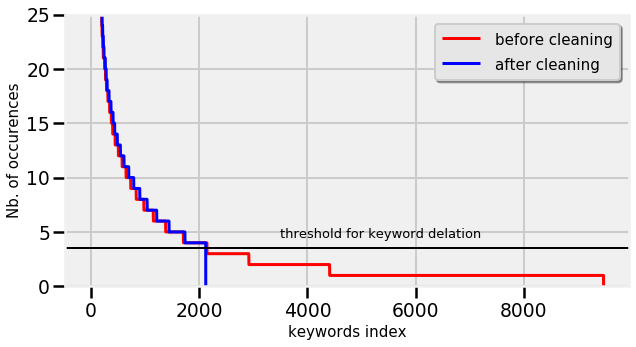
\includegraphics[height=10cm]{./contenido/imagenes/output_64_1.png}
\end{figure}

    { \hspace*{\fill} \\}
    
    \begin{center}\rule{0.5\linewidth}{\linethickness}\end{center}

\subsubsection{2.3 Correlaciones}\label{correlaciones}

    \begin{tcolorbox}[breakable, size=fbox, boxrule=1pt, pad at break*=1mm,colback=cellbackground, colframe=cellborder]
\prompt{In}{incolor}{49}{\hspace{4pt}}
\begin{Verbatim}[commandchars=\\\{\}]
\PY{n}{f}\PY{p}{,} \PY{n}{ax} \PY{o}{=} \PY{n}{plt}\PY{o}{.}\PY{n}{subplots}\PY{p}{(}\PY{n}{figsize}\PY{o}{=}\PY{p}{(}\PY{l+m+mi}{12}\PY{p}{,} \PY{l+m+mi}{9}\PY{p}{)}\PY{p}{)}
\PY{c+c1}{\PYZsh{}\PYZus{}\PYZus{}\PYZus{}\PYZus{}\PYZus{}\PYZus{}\PYZus{}\PYZus{}\PYZus{}\PYZus{}\PYZus{}\PYZus{}\PYZus{}\PYZus{}\PYZus{}\PYZus{}\PYZus{}\PYZus{}\PYZus{}\PYZus{}\PYZus{}\PYZus{}\PYZus{}\PYZus{}\PYZus{}\PYZus{}\PYZus{}\PYZus{}\PYZus{}}
\PY{c+c1}{\PYZsh{} Cálculo de correlaciones}
\PY{n}{corrmat} \PY{o}{=} \PY{n}{df\PYZus{}keywords\PYZus{}occurence}\PY{o}{.}\PY{n}{dropna}\PY{p}{(}\PY{n}{how}\PY{o}{=}\PY{l+s+s1}{\PYZsq{}}\PY{l+s+s1}{any}\PY{l+s+s1}{\PYZsq{}}\PY{p}{)}\PY{o}{.}\PY{n}{corr}\PY{p}{(}\PY{p}{)}
\PY{c+c1}{\PYZsh{}\PYZus{}\PYZus{}\PYZus{}\PYZus{}\PYZus{}\PYZus{}\PYZus{}\PYZus{}\PYZus{}\PYZus{}\PYZus{}\PYZus{}\PYZus{}\PYZus{}\PYZus{}\PYZus{}\PYZus{}\PYZus{}\PYZus{}\PYZus{}\PYZus{}\PYZus{}\PYZus{}\PYZus{}\PYZus{}\PYZus{}\PYZus{}\PYZus{}\PYZus{}\PYZus{}\PYZus{}\PYZus{}\PYZus{}\PYZus{}\PYZus{}\PYZus{}\PYZus{}\PYZus{}\PYZus{}\PYZus{}}
\PY{n}{k} \PY{o}{=} \PY{l+m+mi}{17} \PY{c+c1}{\PYZsh{} number of variables for heatmap}
\PY{n}{cols} \PY{o}{=} \PY{n}{corrmat}\PY{o}{.}\PY{n}{nlargest}\PY{p}{(}\PY{n}{k}\PY{p}{,} \PY{l+s+s1}{\PYZsq{}}\PY{l+s+s1}{num\PYZus{}voted\PYZus{}users}\PY{l+s+s1}{\PYZsq{}}\PY{p}{)}\PY{p}{[}\PY{l+s+s1}{\PYZsq{}}\PY{l+s+s1}{num\PYZus{}voted\PYZus{}users}\PY{l+s+s1}{\PYZsq{}}\PY{p}{]}\PY{o}{.}\PY{n}{index}
\PY{n}{cm} \PY{o}{=} \PY{n}{np}\PY{o}{.}\PY{n}{corrcoef}\PY{p}{(}\PY{n}{df\PYZus{}keywords\PYZus{}occurence}\PY{p}{[}\PY{n}{cols}\PY{p}{]}\PY{o}{.}\PY{n}{dropna}\PY{p}{(}\PY{n}{how}\PY{o}{=}\PY{l+s+s1}{\PYZsq{}}\PY{l+s+s1}{any}\PY{l+s+s1}{\PYZsq{}}\PY{p}{)}\PY{o}{.}\PY{n}{values}\PY{o}{.}\PY{n}{T}\PY{p}{)}
\PY{n}{sns}\PY{o}{.}\PY{n}{set}\PY{p}{(}\PY{n}{font\PYZus{}scale}\PY{o}{=}\PY{l+m+mf}{1.25}\PY{p}{)}
\PY{n}{hm} \PY{o}{=} \PY{n}{sns}\PY{o}{.}\PY{n}{heatmap}\PY{p}{(}\PY{n}{cm}\PY{p}{,} \PY{n}{cbar}\PY{o}{=}\PY{k+kc}{True}\PY{p}{,} \PY{n}{annot}\PY{o}{=}\PY{k+kc}{True}\PY{p}{,} \PY{n}{square}\PY{o}{=}\PY{k+kc}{True}\PY{p}{,}
                 \PY{n}{fmt}\PY{o}{=}\PY{l+s+s1}{\PYZsq{}}\PY{l+s+s1}{.2f}\PY{l+s+s1}{\PYZsq{}}\PY{p}{,} \PY{n}{annot\PYZus{}kws}\PY{o}{=}\PY{p}{\PYZob{}}\PY{l+s+s1}{\PYZsq{}}\PY{l+s+s1}{size}\PY{l+s+s1}{\PYZsq{}}\PY{p}{:} \PY{l+m+mi}{10}\PY{p}{\PYZcb{}}\PY{p}{,} \PY{n}{linewidth} \PY{o}{=} \PY{l+m+mf}{0.1}\PY{p}{,} \PY{n}{cmap} \PY{o}{=} \PY{l+s+s1}{\PYZsq{}}\PY{l+s+s1}{coolwarm}\PY{l+s+s1}{\PYZsq{}}\PY{p}{,}
                 \PY{n}{yticklabels}\PY{o}{=}\PY{n}{cols}\PY{o}{.}\PY{n}{values}\PY{p}{,} \PY{n}{xticklabels}\PY{o}{=}\PY{n}{cols}\PY{o}{.}\PY{n}{values}\PY{p}{)}
\PY{n}{f}\PY{o}{.}\PY{n}{text}\PY{p}{(}\PY{l+m+mf}{0.5}\PY{p}{,} \PY{l+m+mf}{0.93}\PY{p}{,} \PY{l+s+s2}{\PYZdq{}}\PY{l+s+s2}{Coeficientes de correlación}\PY{l+s+s2}{\PYZdq{}}\PY{p}{,} \PY{n}{ha}\PY{o}{=}\PY{l+s+s1}{\PYZsq{}}\PY{l+s+s1}{center}\PY{l+s+s1}{\PYZsq{}}\PY{p}{,} \PY{n}{fontsize} \PY{o}{=} \PY{l+m+mi}{18}\PY{p}{,} \PY{n}{family}\PY{o}{=}\PY{l+s+s1}{\PYZsq{}}\PY{l+s+s1}{fantasy}\PY{l+s+s1}{\PYZsq{}}\PY{p}{)}
\PY{n}{plt}\PY{o}{.}\PY{n}{show}\PY{p}{(}\PY{p}{)}
\end{Verbatim}
\end{tcolorbox}

    \begin{Verbatim}[commandchars=\\\{\}]
findfont: Font family ['fantasy'] not found. Falling back to DejaVu Sans.
findfont: Font family ['fantasy'] not found. Falling back to DejaVu Sans.
\end{Verbatim}

    \begin{center}
    \adjustimage{max size={0.9\linewidth}{0.9\paperheight}}{./contenido/imagenes/output_66_1.png}
    \end{center}
    { \hspace*{\fill} \\}
    
    \begin{tcolorbox}[breakable, size=fbox, boxrule=1pt, pad at break*=1mm,colback=cellbackground, colframe=cellborder]
\prompt{In}{incolor}{50}{\hspace{4pt}}
\begin{Verbatim}[commandchars=\\\{\}]
\PY{n}{LOST\PYZus{}COLUMNS} \PY{o}{=} \PY{p}{[}
    \PY{l+s+s1}{\PYZsq{}}\PY{l+s+s1}{actor\PYZus{}1\PYZus{}facebook\PYZus{}likes}\PY{l+s+s1}{\PYZsq{}}\PY{p}{,}
    \PY{l+s+s1}{\PYZsq{}}\PY{l+s+s1}{actor\PYZus{}2\PYZus{}facebook\PYZus{}likes}\PY{l+s+s1}{\PYZsq{}}\PY{p}{,}
    \PY{l+s+s1}{\PYZsq{}}\PY{l+s+s1}{actor\PYZus{}3\PYZus{}facebook\PYZus{}likes}\PY{l+s+s1}{\PYZsq{}}\PY{p}{,}
    \PY{l+s+s1}{\PYZsq{}}\PY{l+s+s1}{aspect\PYZus{}ratio}\PY{l+s+s1}{\PYZsq{}}\PY{p}{,}
    \PY{l+s+s1}{\PYZsq{}}\PY{l+s+s1}{cast\PYZus{}total\PYZus{}facebook\PYZus{}likes}\PY{l+s+s1}{\PYZsq{}}\PY{p}{,}
    \PY{l+s+s1}{\PYZsq{}}\PY{l+s+s1}{color}\PY{l+s+s1}{\PYZsq{}}\PY{p}{,}
    \PY{l+s+s1}{\PYZsq{}}\PY{l+s+s1}{content\PYZus{}rating}\PY{l+s+s1}{\PYZsq{}}\PY{p}{,}
    \PY{l+s+s1}{\PYZsq{}}\PY{l+s+s1}{director\PYZus{}facebook\PYZus{}likes}\PY{l+s+s1}{\PYZsq{}}\PY{p}{,}
    \PY{l+s+s1}{\PYZsq{}}\PY{l+s+s1}{facenumber\PYZus{}in\PYZus{}poster}\PY{l+s+s1}{\PYZsq{}}\PY{p}{,}
    \PY{l+s+s1}{\PYZsq{}}\PY{l+s+s1}{movie\PYZus{}facebook\PYZus{}likes}\PY{l+s+s1}{\PYZsq{}}\PY{p}{,}
    \PY{l+s+s1}{\PYZsq{}}\PY{l+s+s1}{movie\PYZus{}imdb\PYZus{}link}\PY{l+s+s1}{\PYZsq{}}\PY{p}{,}
    \PY{l+s+s1}{\PYZsq{}}\PY{l+s+s1}{num\PYZus{}critic\PYZus{}for\PYZus{}reviews}\PY{l+s+s1}{\PYZsq{}}\PY{p}{,}
    \PY{l+s+s1}{\PYZsq{}}\PY{l+s+s1}{num\PYZus{}user\PYZus{}for\PYZus{}reviews}\PY{l+s+s1}{\PYZsq{}}
                \PY{p}{]}
\end{Verbatim}
\end{tcolorbox}

    \begin{tcolorbox}[breakable, size=fbox, boxrule=1pt, pad at break*=1mm,colback=cellbackground, colframe=cellborder]
\prompt{In}{incolor}{51}{\hspace{4pt}}
\begin{Verbatim}[commandchars=\\\{\}]
\PY{c+c1}{\PYZsh{}\PYZus{}\PYZus{}\PYZus{}\PYZus{}\PYZus{}\PYZus{}\PYZus{}\PYZus{}\PYZus{}\PYZus{}}
\PY{c+c1}{\PYZsh{} dropping}
\PY{c+c1}{\PYZsh{}dropped\PYZus{}var = [\PYZsq{}aspect\PYZus{}ratio\PYZsq{}, \PYZsq{}budget\PYZsq{}, \PYZsq{}facenumber\PYZus{}in\PYZus{}poster\PYZsq{},}
\PY{c+c1}{\PYZsh{}               \PYZsq{}content\PYZus{}rating\PYZsq{}, \PYZsq{}cast\PYZus{}total\PYZus{}facebook\PYZus{}likes\PYZsq{}]}
\PY{c+c1}{\PYZsh{}df\PYZus{}var\PYZus{}cleaned = df\PYZus{}keywords\PYZus{}occurence.drop(dropped\PYZus{}var, axis = 1)}
\PY{c+c1}{\PYZsh{}\PYZus{}\PYZus{}\PYZus{}\PYZus{}\PYZus{}\PYZus{}\PYZus{}\PYZus{}\PYZus{}\PYZus{}\PYZus{}\PYZus{}\PYZus{}\PYZus{}\PYZus{}\PYZus{}}
\PY{c+c1}{\PYZsh{} and reordering}
\PY{n}{new\PYZus{}col\PYZus{}order} \PY{o}{=} \PY{p}{[}\PY{l+s+s1}{\PYZsq{}}\PY{l+s+s1}{movie\PYZus{}title}\PY{l+s+s1}{\PYZsq{}}\PY{p}{,} \PY{l+s+s1}{\PYZsq{}}\PY{l+s+s1}{title\PYZus{}year}\PY{l+s+s1}{\PYZsq{}}\PY{p}{,} \PY{l+s+s1}{\PYZsq{}}\PY{l+s+s1}{genres}\PY{l+s+s1}{\PYZsq{}}\PY{p}{,} \PY{l+s+s1}{\PYZsq{}}\PY{l+s+s1}{plot\PYZus{}keywords}\PY{l+s+s1}{\PYZsq{}}\PY{p}{,} 
                 \PY{l+s+s1}{\PYZsq{}}\PY{l+s+s1}{director\PYZus{}name}\PY{l+s+s1}{\PYZsq{}}\PY{p}{,} \PY{l+s+s1}{\PYZsq{}}\PY{l+s+s1}{actor\PYZus{}1\PYZus{}name}\PY{l+s+s1}{\PYZsq{}}\PY{p}{,} \PY{l+s+s1}{\PYZsq{}}\PY{l+s+s1}{actor\PYZus{}2\PYZus{}name}\PY{l+s+s1}{\PYZsq{}}\PY{p}{,} \PY{l+s+s1}{\PYZsq{}}\PY{l+s+s1}{actor\PYZus{}3\PYZus{}name}\PY{l+s+s1}{\PYZsq{}}\PY{p}{,}
                 \PY{l+s+s1}{\PYZsq{}}\PY{l+s+s1}{director\PYZus{}facebook\PYZus{}likes}\PY{l+s+s1}{\PYZsq{}}\PY{p}{,} \PY{l+s+s1}{\PYZsq{}}\PY{l+s+s1}{actor\PYZus{}1\PYZus{}facebook\PYZus{}likes}\PY{l+s+s1}{\PYZsq{}}\PY{p}{,} \PY{l+s+s1}{\PYZsq{}}\PY{l+s+s1}{actor\PYZus{}2\PYZus{}facebook\PYZus{}likes}\PY{l+s+s1}{\PYZsq{}}\PY{p}{,}
                 \PY{l+s+s1}{\PYZsq{}}\PY{l+s+s1}{actor\PYZus{}3\PYZus{}facebook\PYZus{}likes}\PY{l+s+s1}{\PYZsq{}}\PY{p}{,} \PY{l+s+s1}{\PYZsq{}}\PY{l+s+s1}{movie\PYZus{}facebook\PYZus{}likes}\PY{l+s+s1}{\PYZsq{}}\PY{p}{,} \PY{l+s+s1}{\PYZsq{}}\PY{l+s+s1}{num\PYZus{}critic\PYZus{}for\PYZus{}reviews}\PY{l+s+s1}{\PYZsq{}}\PY{p}{,} 
                 \PY{l+s+s1}{\PYZsq{}}\PY{l+s+s1}{num\PYZus{}user\PYZus{}for\PYZus{}reviews}\PY{l+s+s1}{\PYZsq{}}\PY{p}{,} \PY{l+s+s1}{\PYZsq{}}\PY{l+s+s1}{num\PYZus{}voted\PYZus{}users}\PY{l+s+s1}{\PYZsq{}}\PY{p}{,} \PY{l+s+s1}{\PYZsq{}}\PY{l+s+s1}{language}\PY{l+s+s1}{\PYZsq{}}\PY{p}{,} \PY{l+s+s1}{\PYZsq{}}\PY{l+s+s1}{country}\PY{l+s+s1}{\PYZsq{}}\PY{p}{,}
                 \PY{l+s+s1}{\PYZsq{}}\PY{l+s+s1}{imdb\PYZus{}score}\PY{l+s+s1}{\PYZsq{}}\PY{p}{,} \PY{l+s+s1}{\PYZsq{}}\PY{l+s+s1}{movie\PYZus{}imdb\PYZus{}link}\PY{l+s+s1}{\PYZsq{}}\PY{p}{,} \PY{l+s+s1}{\PYZsq{}}\PY{l+s+s1}{color}\PY{l+s+s1}{\PYZsq{}}\PY{p}{,} \PY{l+s+s1}{\PYZsq{}}\PY{l+s+s1}{duration}\PY{l+s+s1}{\PYZsq{}}\PY{p}{,} \PY{l+s+s1}{\PYZsq{}}\PY{l+s+s1}{gross}\PY{l+s+s1}{\PYZsq{}}\PY{p}{,} \PY{p}{]}
\PY{n}{new\PYZus{}col\PYZus{}order} \PY{o}{=} \PY{p}{[}\PY{n}{col} \PY{k}{for} \PY{n}{col} \PY{o+ow}{in} \PY{n}{new\PYZus{}col\PYZus{}order} \PY{k}{if} \PY{n}{col} \PY{o+ow}{not} \PY{o+ow}{in} \PY{n}{LOST\PYZus{}COLUMNS}\PY{p}{]}
\PY{n+nb}{print}\PY{p}{(}\PY{n}{new\PYZus{}col\PYZus{}order}\PY{p}{)}
\PY{n}{new\PYZus{}col\PYZus{}order} \PY{o}{=} \PY{p}{[}\PY{n}{IMDB\PYZus{}COLUMNS\PYZus{}TO\PYZus{}REMAP}\PY{p}{[}\PY{n}{col}\PY{p}{]} \PY{k}{if} \PY{n}{col} \PY{o+ow}{in} \PY{n}{IMDB\PYZus{}COLUMNS\PYZus{}TO\PYZus{}REMAP} \PY{k}{else} \PY{n}{col}
                 \PY{k}{for} \PY{n}{col} \PY{o+ow}{in} \PY{n}{new\PYZus{}col\PYZus{}order}\PY{p}{]}
\PY{n+nb}{print}\PY{p}{(}\PY{n}{new\PYZus{}col\PYZus{}order}\PY{p}{)}
\PY{n}{new\PYZus{}col\PYZus{}order} \PY{o}{=} \PY{p}{[}\PY{n}{TMDB\PYZus{}TO\PYZus{}IMDB\PYZus{}SIMPLE\PYZus{}EQUIVALENCIES}\PY{p}{[}\PY{n}{col}\PY{p}{]} \PY{k}{if} \PY{n}{col} \PY{o+ow}{in} \PY{n}{TMDB\PYZus{}TO\PYZus{}IMDB\PYZus{}SIMPLE\PYZus{}EQUIVALENCIES} \PY{k}{else} \PY{n}{col}
                 \PY{k}{for} \PY{n}{col} \PY{o+ow}{in} \PY{n}{new\PYZus{}col\PYZus{}order}\PY{p}{]}
\PY{n+nb}{print}\PY{p}{(}\PY{n}{new\PYZus{}col\PYZus{}order}\PY{p}{)}
\PY{n}{df\PYZus{}var\PYZus{}cleaned} \PY{o}{=} \PY{n}{df\PYZus{}keywords\PYZus{}occurence}\PY{p}{[}\PY{n}{new\PYZus{}col\PYZus{}order}\PY{p}{]}
\end{Verbatim}
\end{tcolorbox}

    \begin{Verbatim}[commandchars=\\\{\}]
['movie\_title', 'title\_year', 'genres', 'plot\_keywords', 'director\_name',
'actor\_1\_name', 'actor\_2\_name', 'actor\_3\_name', 'num\_voted\_users', 'language',
'country', 'imdb\_score', 'duration', 'gross']
['movie\_title', 'title\_year', 'genres', 'plot\_keywords', 'director\_name',
'actor\_1\_name', 'actor\_2\_name', 'actor\_3\_name', 'num\_voted\_users', 'language',
'country', 'vote\_average', 'duration', 'gross']
['movie\_title', 'title\_year', 'genres', 'plot\_keywords', 'director\_name',
'actor\_1\_name', 'actor\_2\_name', 'actor\_3\_name', 'num\_voted\_users', 'language',
'country', 'vote\_average', 'duration', 'gross']
\end{Verbatim}

    \begin{tcolorbox}[breakable, size=fbox, boxrule=1pt, pad at break*=1mm,colback=cellbackground, colframe=cellborder]
\prompt{In}{incolor}{52}{\hspace{4pt}}
\begin{Verbatim}[commandchars=\\\{\}]
\PY{n}{set2} \PY{o}{=} \PY{n+nb}{set}\PY{p}{(}\PY{n+nb}{list}\PY{p}{(}\PY{n}{df\PYZus{}var\PYZus{}cleaned}\PY{o}{.}\PY{n}{columns}\PY{p}{)}\PY{p}{)}
\end{Verbatim}
\end{tcolorbox}

    \begin{tcolorbox}[breakable, size=fbox, boxrule=1pt, pad at break*=1mm,colback=cellbackground, colframe=cellborder]
\prompt{In}{incolor}{53}{\hspace{4pt}}
\begin{Verbatim}[commandchars=\\\{\}]
\PY{n}{set1} \PY{o}{=} \PY{n+nb}{set}\PY{p}{(}\PY{n+nb}{list}\PY{p}{(}\PY{n}{df\PYZus{}keywords\PYZus{}occurence}\PY{o}{.}\PY{n}{columns}\PY{p}{)}\PY{p}{)}
\PY{n}{set1}\PY{o}{.}\PY{n}{difference}\PY{p}{(}\PY{n+nb}{list}\PY{p}{(}\PY{n}{df\PYZus{}var\PYZus{}cleaned}\PY{o}{.}\PY{n}{columns}\PY{p}{)}\PY{p}{)}
\end{Verbatim}
\end{tcolorbox}

            \begin{tcolorbox}[breakable, boxrule=.5pt, size=fbox, pad at break*=1mm, opacityfill=0]
\prompt{Out}{outcolor}{53}{\hspace{3.5pt}}
\begin{Verbatim}[commandchars=\\\{\}]
\{'budget',
 'homepage',
 'id',
 'original\_title',
 'overview',
 'popularity',
 'production\_companies',
 'production\_countries',
 'release\_date',
 'spoken\_languages',
 'status',
 'tagline'\}
\end{Verbatim}
\end{tcolorbox}
        
    \begin{center}\rule{0.5\linewidth}{\linethickness}\end{center}

\subsubsection{2.4 Valores faltantes}\label{valores-faltantes}

Examinamos el número de valores faltantes en cada variable y escogemos
una metodología para completar el dataset.

    \begin{tcolorbox}[breakable, size=fbox, boxrule=1pt, pad at break*=1mm,colback=cellbackground, colframe=cellborder]
\prompt{In}{incolor}{54}{\hspace{4pt}}
\begin{Verbatim}[commandchars=\\\{\}]
\PY{n}{missing\PYZus{}df} \PY{o}{=} \PY{n}{df\PYZus{}var\PYZus{}cleaned}\PY{o}{.}\PY{n}{isnull}\PY{p}{(}\PY{p}{)}\PY{o}{.}\PY{n}{sum}\PY{p}{(}\PY{n}{axis}\PY{o}{=}\PY{l+m+mi}{0}\PY{p}{)}\PY{o}{.}\PY{n}{reset\PYZus{}index}\PY{p}{(}\PY{p}{)}
\PY{n}{missing\PYZus{}df}\PY{o}{.}\PY{n}{columns} \PY{o}{=} \PY{p}{[}\PY{l+s+s1}{\PYZsq{}}\PY{l+s+s1}{column\PYZus{}name}\PY{l+s+s1}{\PYZsq{}}\PY{p}{,} \PY{l+s+s1}{\PYZsq{}}\PY{l+s+s1}{missing\PYZus{}count}\PY{l+s+s1}{\PYZsq{}}\PY{p}{]}
\PY{n}{missing\PYZus{}df}\PY{p}{[}\PY{l+s+s1}{\PYZsq{}}\PY{l+s+s1}{filling\PYZus{}factor}\PY{l+s+s1}{\PYZsq{}}\PY{p}{]} \PY{o}{=} \PY{p}{(}\PY{n}{df\PYZus{}var\PYZus{}cleaned}\PY{o}{.}\PY{n}{shape}\PY{p}{[}\PY{l+m+mi}{0}\PY{p}{]} 
                                \PY{o}{\PYZhy{}} \PY{n}{missing\PYZus{}df}\PY{p}{[}\PY{l+s+s1}{\PYZsq{}}\PY{l+s+s1}{missing\PYZus{}count}\PY{l+s+s1}{\PYZsq{}}\PY{p}{]}\PY{p}{)} \PY{o}{/} \PY{n}{df\PYZus{}var\PYZus{}cleaned}\PY{o}{.}\PY{n}{shape}\PY{p}{[}\PY{l+m+mi}{0}\PY{p}{]} \PY{o}{*} \PY{l+m+mi}{100}
\PY{n}{missing\PYZus{}df} \PY{o}{=} \PY{n}{missing\PYZus{}df}\PY{o}{.}\PY{n}{sort\PYZus{}values}\PY{p}{(}\PY{l+s+s1}{\PYZsq{}}\PY{l+s+s1}{filling\PYZus{}factor}\PY{l+s+s1}{\PYZsq{}}\PY{p}{)}\PY{o}{.}\PY{n}{reset\PYZus{}index}\PY{p}{(}\PY{n}{drop} \PY{o}{=} \PY{k+kc}{True}\PY{p}{)}
\PY{n}{missing\PYZus{}df}
\end{Verbatim}
\end{tcolorbox}

            \begin{tcolorbox}[breakable, boxrule=.5pt, size=fbox, pad at break*=1mm, opacityfill=0]
\prompt{Out}{outcolor}{54}{\hspace{3.5pt}}
\begin{Verbatim}[commandchars=\\\{\}]
        column\_name  missing\_count  filling\_factor
0           country            174       96.377264
1      actor\_3\_name             93       98.063710
2          language             86       98.209452
3      actor\_2\_name             63       98.688320
4      actor\_1\_name             53       98.896523
5     director\_name             30       99.375390
6          duration              2       99.958359
7        title\_year              1       99.979180
8       movie\_title              0      100.000000
9            genres              0      100.000000
10    plot\_keywords              0      100.000000
11  num\_voted\_users              0      100.000000
12     vote\_average              0      100.000000
13            gross              0      100.000000
\end{Verbatim}
\end{tcolorbox}
        
    Ahora representamos el contenido de esta tabla:

    \begin{tcolorbox}[breakable, size=fbox, boxrule=1pt, pad at break*=1mm,colback=cellbackground, colframe=cellborder]
\prompt{In}{incolor}{55}{\hspace{4pt}}
\begin{Verbatim}[commandchars=\\\{\}]
\PY{n}{y\PYZus{}axis} \PY{o}{=} \PY{n}{missing\PYZus{}df}\PY{p}{[}\PY{l+s+s1}{\PYZsq{}}\PY{l+s+s1}{filling\PYZus{}factor}\PY{l+s+s1}{\PYZsq{}}\PY{p}{]} 
\PY{n}{x\PYZus{}label} \PY{o}{=} \PY{n}{missing\PYZus{}df}\PY{p}{[}\PY{l+s+s1}{\PYZsq{}}\PY{l+s+s1}{column\PYZus{}name}\PY{l+s+s1}{\PYZsq{}}\PY{p}{]}
\PY{n}{x\PYZus{}axis} \PY{o}{=} \PY{n}{missing\PYZus{}df}\PY{o}{.}\PY{n}{index}

\PY{n}{fig} \PY{o}{=} \PY{n}{plt}\PY{o}{.}\PY{n}{figure}\PY{p}{(}\PY{n}{figsize}\PY{o}{=}\PY{p}{(}\PY{l+m+mi}{11}\PY{p}{,} \PY{l+m+mi}{4}\PY{p}{)}\PY{p}{)}
\PY{n}{plt}\PY{o}{.}\PY{n}{xticks}\PY{p}{(}\PY{n}{rotation}\PY{o}{=}\PY{l+m+mi}{80}\PY{p}{,} \PY{n}{fontsize} \PY{o}{=} \PY{l+m+mi}{14}\PY{p}{)}
\PY{n}{plt}\PY{o}{.}\PY{n}{yticks}\PY{p}{(}\PY{n}{fontsize} \PY{o}{=} \PY{l+m+mi}{13}\PY{p}{)}

\PY{n}{N\PYZus{}thresh} \PY{o}{=} \PY{l+m+mi}{5}
\PY{n}{plt}\PY{o}{.}\PY{n}{axvline}\PY{p}{(}\PY{n}{x}\PY{o}{=}\PY{n}{N\PYZus{}thresh}\PY{o}{\PYZhy{}}\PY{l+m+mf}{0.5}\PY{p}{,} \PY{n}{linewidth}\PY{o}{=}\PY{l+m+mi}{2}\PY{p}{,} \PY{n}{color} \PY{o}{=} \PY{l+s+s1}{\PYZsq{}}\PY{l+s+s1}{r}\PY{l+s+s1}{\PYZsq{}}\PY{p}{)}
\PY{n}{plt}\PY{o}{.}\PY{n}{text}\PY{p}{(}\PY{n}{N\PYZus{}thresh}\PY{o}{\PYZhy{}}\PY{l+m+mf}{4.8}\PY{p}{,} \PY{l+m+mi}{30}\PY{p}{,} \PY{l+s+s1}{\PYZsq{}}\PY{l+s+s1}{factor completitud }\PY{l+s+se}{\PYZbs{}n}\PY{l+s+s1}{ \PYZlt{} }\PY{l+s+si}{\PYZob{}\PYZcb{}}\PY{l+s+s1}{\PYZpc{}}\PY{l+s+s1}{\PYZsq{}}\PY{o}{.}\PY{n}{format}\PY{p}{(}\PY{n+nb}{round}\PY{p}{(}\PY{n}{y\PYZus{}axis}\PY{p}{[}\PY{n}{N\PYZus{}thresh}\PY{p}{]}\PY{p}{,}\PY{l+m+mi}{1}\PY{p}{)}\PY{p}{)}\PY{p}{,}
         \PY{n}{fontsize} \PY{o}{=} \PY{l+m+mi}{15}\PY{p}{,} \PY{n}{family} \PY{o}{=} \PY{l+s+s1}{\PYZsq{}}\PY{l+s+s1}{fantasy}\PY{l+s+s1}{\PYZsq{}}\PY{p}{,} \PY{n}{bbox}\PY{o}{=}\PY{n+nb}{dict}\PY{p}{(}\PY{n}{boxstyle}\PY{o}{=}\PY{l+s+s2}{\PYZdq{}}\PY{l+s+s2}{round}\PY{l+s+s2}{\PYZdq{}}\PY{p}{,}
                   \PY{n}{ec}\PY{o}{=}\PY{p}{(}\PY{l+m+mf}{1.0}\PY{p}{,} \PY{l+m+mf}{0.5}\PY{p}{,} \PY{l+m+mf}{0.5}\PY{p}{)}\PY{p}{,}
                   \PY{n}{fc}\PY{o}{=}\PY{p}{(}\PY{l+m+mf}{0.8}\PY{p}{,} \PY{l+m+mf}{0.5}\PY{p}{,} \PY{l+m+mf}{0.5}\PY{p}{)}\PY{p}{)}\PY{p}{)}
\PY{n}{N\PYZus{}thresh} \PY{o}{=} \PY{l+m+mi}{13}
\PY{n}{plt}\PY{o}{.}\PY{n}{axvline}\PY{p}{(}\PY{n}{x}\PY{o}{=}\PY{n}{N\PYZus{}thresh}\PY{o}{\PYZhy{}}\PY{l+m+mf}{0.5}\PY{p}{,} \PY{n}{linewidth}\PY{o}{=}\PY{l+m+mi}{2}\PY{p}{,} \PY{n}{color} \PY{o}{=} \PY{l+s+s1}{\PYZsq{}}\PY{l+s+s1}{g}\PY{l+s+s1}{\PYZsq{}}\PY{p}{)}
\PY{n}{plt}\PY{o}{.}\PY{n}{text}\PY{p}{(}\PY{n}{N\PYZus{}thresh}\PY{p}{,} \PY{l+m+mi}{30}\PY{p}{,} \PY{l+s+s1}{\PYZsq{}}\PY{l+s+s1}{factor completitud }\PY{l+s+se}{\PYZbs{}n}\PY{l+s+s1}{ = }\PY{l+s+si}{\PYZob{}\PYZcb{}}\PY{l+s+s1}{\PYZpc{}}\PY{l+s+s1}{\PYZsq{}}\PY{o}{.}\PY{n}{format}\PY{p}{(}\PY{n+nb}{round}\PY{p}{(}\PY{n}{y\PYZus{}axis}\PY{p}{[}\PY{n}{N\PYZus{}thresh}\PY{p}{]}\PY{p}{,}\PY{l+m+mi}{1}\PY{p}{)}\PY{p}{)}\PY{p}{,}
         \PY{n}{fontsize} \PY{o}{=} \PY{l+m+mi}{15}\PY{p}{,} \PY{n}{family} \PY{o}{=} \PY{l+s+s1}{\PYZsq{}}\PY{l+s+s1}{fantasy}\PY{l+s+s1}{\PYZsq{}}\PY{p}{,} \PY{n}{bbox}\PY{o}{=}\PY{n+nb}{dict}\PY{p}{(}\PY{n}{boxstyle}\PY{o}{=}\PY{l+s+s2}{\PYZdq{}}\PY{l+s+s2}{round}\PY{l+s+s2}{\PYZdq{}}\PY{p}{,}
                   \PY{n}{ec}\PY{o}{=}\PY{p}{(}\PY{l+m+mf}{1.}\PY{p}{,} \PY{l+m+mf}{0.5}\PY{p}{,} \PY{l+m+mf}{0.5}\PY{p}{)}\PY{p}{,}
                   \PY{n}{fc}\PY{o}{=}\PY{p}{(}\PY{l+m+mf}{0.5}\PY{p}{,} \PY{l+m+mf}{0.8}\PY{p}{,} \PY{l+m+mf}{0.5}\PY{p}{)}\PY{p}{)}\PY{p}{)}

\PY{n}{plt}\PY{o}{.}\PY{n}{xticks}\PY{p}{(}\PY{n}{x\PYZus{}axis}\PY{p}{,} \PY{n}{x\PYZus{}label}\PY{p}{,}\PY{n}{family}\PY{o}{=}\PY{l+s+s1}{\PYZsq{}}\PY{l+s+s1}{fantasy}\PY{l+s+s1}{\PYZsq{}}\PY{p}{,} \PY{n}{fontsize} \PY{o}{=} \PY{l+m+mi}{14} \PY{p}{)}
\PY{n}{plt}\PY{o}{.}\PY{n}{ylabel}\PY{p}{(}\PY{l+s+s1}{\PYZsq{}}\PY{l+s+s1}{Factor de completitud (}\PY{l+s+s1}{\PYZpc{}}\PY{l+s+s1}{)}\PY{l+s+s1}{\PYZsq{}}\PY{p}{,} \PY{n}{family}\PY{o}{=}\PY{l+s+s1}{\PYZsq{}}\PY{l+s+s1}{fantasy}\PY{l+s+s1}{\PYZsq{}}\PY{p}{,} \PY{n}{fontsize} \PY{o}{=} \PY{l+m+mi}{16}\PY{p}{)}
\PY{n}{plt}\PY{o}{.}\PY{n}{bar}\PY{p}{(}\PY{n}{x\PYZus{}axis}\PY{p}{,} \PY{n}{y\PYZus{}axis}\PY{p}{)}\PY{p}{;}
\end{Verbatim}
\end{tcolorbox}

    \begin{Verbatim}[commandchars=\\\{\}]
findfont: Font family ['fantasy'] not found. Falling back to DejaVu Sans.
findfont: Font family ['fantasy'] not found. Falling back to DejaVu Sans.
findfont: Font family ['fantasy'] not found. Falling back to DejaVu Sans.
\end{Verbatim}

\begin{figure}[h]
    \centering
    \captionsetup{width=10cm}
    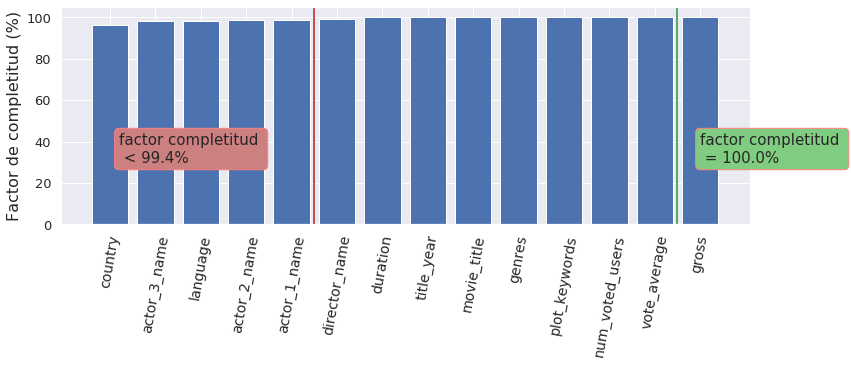
\includegraphics[height=10cm]{./contenido/imagenes/output_74_1.png}
\end{figure}
    { \hspace*{\fill} \\}
    
    \begin{center}\rule{0.5\linewidth}{\linethickness}\end{center}

\paragraph{2.4.1 Completando los años
faltantes}\label{completando-los-auxf1os-faltantes}

Para inferir el año de la película, se usan los actores y el director.
Para cada uno de ellos, determinamos el año medio de actividad,
utilizando el dataset que tenemos. A continuación, se promedian los
valores para determinar el año de la película.

To infer the title year, I use the list of actors and the director. For
each of them, I determine the mean year of activity, using the current
dataset. I then average the values obtained to estimate the title year.

    \begin{tcolorbox}[breakable, size=fbox, boxrule=1pt, pad at break*=1mm,colback=cellbackground, colframe=cellborder]
\prompt{In}{incolor}{56}{\hspace{4pt}}
\begin{Verbatim}[commandchars=\\\{\}]
\PY{n}{df\PYZus{}filling} \PY{o}{=} \PY{n}{df\PYZus{}var\PYZus{}cleaned}\PY{o}{.}\PY{n}{copy}\PY{p}{(}\PY{n}{deep}\PY{o}{=}\PY{k+kc}{True}\PY{p}{)}
\PY{n}{missing\PYZus{}year\PYZus{}info} \PY{o}{=} \PY{n}{df\PYZus{}filling}\PY{p}{[}\PY{n}{df\PYZus{}filling}\PY{p}{[}\PY{l+s+s1}{\PYZsq{}}\PY{l+s+s1}{title\PYZus{}year}\PY{l+s+s1}{\PYZsq{}}\PY{p}{]}\PY{o}{.}\PY{n}{isnull}\PY{p}{(}\PY{p}{)}\PY{p}{]}\PY{p}{[}\PY{p}{[}
            \PY{l+s+s1}{\PYZsq{}}\PY{l+s+s1}{director\PYZus{}name}\PY{l+s+s1}{\PYZsq{}}\PY{p}{,}\PY{l+s+s1}{\PYZsq{}}\PY{l+s+s1}{actor\PYZus{}1\PYZus{}name}\PY{l+s+s1}{\PYZsq{}}\PY{p}{,} \PY{l+s+s1}{\PYZsq{}}\PY{l+s+s1}{actor\PYZus{}2\PYZus{}name}\PY{l+s+s1}{\PYZsq{}}\PY{p}{,} \PY{l+s+s1}{\PYZsq{}}\PY{l+s+s1}{actor\PYZus{}3\PYZus{}name}\PY{l+s+s1}{\PYZsq{}}\PY{p}{]}\PY{p}{]}
\PY{n}{missing\PYZus{}year\PYZus{}info}\PY{p}{[}\PY{p}{:}\PY{l+m+mi}{10}\PY{p}{]}
\end{Verbatim}
\end{tcolorbox}

            \begin{tcolorbox}[breakable, boxrule=.5pt, size=fbox, pad at break*=1mm, opacityfill=0]
\prompt{Out}{outcolor}{56}{\hspace{3.5pt}}
\begin{Verbatim}[commandchars=\\\{\}]
     director\_name actor\_1\_name actor\_2\_name actor\_3\_name
4553           NaN          NaN          NaN          NaN
\end{Verbatim}
\end{tcolorbox}
        
    \begin{tcolorbox}[breakable, size=fbox, boxrule=1pt, pad at break*=1mm,colback=cellbackground, colframe=cellborder]
\prompt{In}{incolor}{57}{\hspace{4pt}}
\begin{Verbatim}[commandchars=\\\{\}]
\PY{k}{def} \PY{n+nf}{fill\PYZus{}year}\PY{p}{(}\PY{n}{df}\PY{p}{)}\PY{p}{:}
    \PY{l+s+sd}{\PYZdq{}\PYZdq{}\PYZdq{}Completa la columna faltante del año teniendo en cuenta la media}
\PY{l+s+sd}{    de los periodos de actividad de los actores y el director.}
\PY{l+s+sd}{    \PYZdq{}\PYZdq{}\PYZdq{}}
    \PY{n}{col} \PY{o}{=} \PY{p}{[}\PY{l+s+s1}{\PYZsq{}}\PY{l+s+s1}{director\PYZus{}name}\PY{l+s+s1}{\PYZsq{}}\PY{p}{,} \PY{l+s+s1}{\PYZsq{}}\PY{l+s+s1}{actor\PYZus{}1\PYZus{}name}\PY{l+s+s1}{\PYZsq{}}\PY{p}{,} \PY{l+s+s1}{\PYZsq{}}\PY{l+s+s1}{actor\PYZus{}2\PYZus{}name}\PY{l+s+s1}{\PYZsq{}}\PY{p}{,} \PY{l+s+s1}{\PYZsq{}}\PY{l+s+s1}{actor\PYZus{}3\PYZus{}name}\PY{l+s+s1}{\PYZsq{}}\PY{p}{]}
    \PY{n}{usual\PYZus{}year} \PY{o}{=} \PY{p}{[}\PY{l+m+mi}{0} \PY{k}{for} \PY{n}{\PYZus{}} \PY{o+ow}{in} \PY{n+nb}{range}\PY{p}{(}\PY{l+m+mi}{4}\PY{p}{)}\PY{p}{]}
    \PY{n}{var}        \PY{o}{=} \PY{p}{[}\PY{l+m+mi}{0} \PY{k}{for} \PY{n}{\PYZus{}} \PY{o+ow}{in} \PY{n+nb}{range}\PY{p}{(}\PY{l+m+mi}{4}\PY{p}{)}\PY{p}{]}
    \PY{c+c1}{\PYZsh{}\PYZus{}\PYZus{}\PYZus{}\PYZus{}\PYZus{}\PYZus{}\PYZus{}\PYZus{}\PYZus{}\PYZus{}\PYZus{}\PYZus{}\PYZus{}\PYZus{}\PYZus{}\PYZus{}\PYZus{}\PYZus{}\PYZus{}\PYZus{}\PYZus{}\PYZus{}\PYZus{}\PYZus{}\PYZus{}\PYZus{}\PYZus{}\PYZus{}\PYZus{}\PYZus{}\PYZus{}\PYZus{}\PYZus{}\PYZus{}\PYZus{}\PYZus{}\PYZus{}\PYZus{}\PYZus{}\PYZus{}\PYZus{}\PYZus{}\PYZus{}\PYZus{}\PYZus{}\PYZus{}\PYZus{}\PYZus{}\PYZus{}\PYZus{}\PYZus{}\PYZus{}\PYZus{}\PYZus{}\PYZus{}\PYZus{}\PYZus{}\PYZus{}\PYZus{}\PYZus{}\PYZus{}}
    \PY{c+c1}{\PYZsh{} Año medio de actividad para los actores y el director}
    \PY{k}{for} \PY{n}{i} \PY{o+ow}{in} \PY{n+nb}{range}\PY{p}{(}\PY{n+nb}{len}\PY{p}{(}\PY{n}{col}\PY{p}{)}\PY{p}{)}\PY{p}{:}
        \PY{n}{usual\PYZus{}year}\PY{p}{[}\PY{n}{i}\PY{p}{]} \PY{o}{=} \PY{n}{df}\PY{o}{.}\PY{n}{groupby}\PY{p}{(}\PY{n}{col}\PY{p}{[}\PY{n}{i}\PY{p}{]}\PY{p}{)}\PY{p}{[}\PY{l+s+s1}{\PYZsq{}}\PY{l+s+s1}{title\PYZus{}year}\PY{l+s+s1}{\PYZsq{}}\PY{p}{]}\PY{o}{.}\PY{n}{mean}\PY{p}{(}\PY{p}{)}
    \PY{c+c1}{\PYZsh{}\PYZus{}\PYZus{}\PYZus{}\PYZus{}\PYZus{}\PYZus{}\PYZus{}\PYZus{}\PYZus{}\PYZus{}\PYZus{}\PYZus{}\PYZus{}\PYZus{}\PYZus{}\PYZus{}\PYZus{}\PYZus{}\PYZus{}\PYZus{}\PYZus{}\PYZus{}\PYZus{}\PYZus{}\PYZus{}\PYZus{}\PYZus{}\PYZus{}\PYZus{}\PYZus{}\PYZus{}\PYZus{}\PYZus{}\PYZus{}\PYZus{}\PYZus{}\PYZus{}\PYZus{}\PYZus{}\PYZus{}\PYZus{}\PYZus{}\PYZus{}\PYZus{}\PYZus{}}
    \PY{c+c1}{\PYZsh{} Diccionario que recoja esta información}
    \PY{n}{actor\PYZus{}year} \PY{o}{=} \PY{n+nb}{dict}\PY{p}{(}\PY{p}{)}
    \PY{k}{for} \PY{n}{i} \PY{o+ow}{in} \PY{n+nb}{range}\PY{p}{(}\PY{l+m+mi}{4}\PY{p}{)}\PY{p}{:}
        \PY{k}{for} \PY{n}{s} \PY{o+ow}{in} \PY{n}{usual\PYZus{}year}\PY{p}{[}\PY{n}{i}\PY{p}{]}\PY{o}{.}\PY{n}{index}\PY{p}{:}
            \PY{k}{if} \PY{n}{s} \PY{o+ow}{in} \PY{n}{actor\PYZus{}year}\PY{o}{.}\PY{n}{keys}\PY{p}{(}\PY{p}{)}\PY{p}{:}
                \PY{k}{if} \PY{n}{pd}\PY{o}{.}\PY{n}{notnull}\PY{p}{(}\PY{n}{usual\PYZus{}year}\PY{p}{[}\PY{n}{i}\PY{p}{]}\PY{p}{[}\PY{n}{s}\PY{p}{]}\PY{p}{)} \PY{o+ow}{and} \PY{n}{pd}\PY{o}{.}\PY{n}{notnull}\PY{p}{(}\PY{n}{actor\PYZus{}year}\PY{p}{[}\PY{n}{s}\PY{p}{]}\PY{p}{)}\PY{p}{:}
                    \PY{n}{actor\PYZus{}year}\PY{p}{[}\PY{n}{s}\PY{p}{]} \PY{o}{=} \PY{p}{(}\PY{n}{actor\PYZus{}year}\PY{p}{[}\PY{n}{s}\PY{p}{]} \PY{o}{+} \PY{n}{usual\PYZus{}year}\PY{p}{[}\PY{n}{i}\PY{p}{]}\PY{p}{[}\PY{n}{s}\PY{p}{]}\PY{p}{)}\PY{o}{/}\PY{l+m+mi}{2}
                \PY{k}{elif} \PY{n}{pd}\PY{o}{.}\PY{n}{isnull}\PY{p}{(}\PY{n}{actor\PYZus{}year}\PY{p}{[}\PY{n}{s}\PY{p}{]}\PY{p}{)}\PY{p}{:}
                    \PY{n}{actor\PYZus{}year}\PY{p}{[}\PY{n}{s}\PY{p}{]} \PY{o}{=} \PY{n}{usual\PYZus{}year}\PY{p}{[}\PY{n}{i}\PY{p}{]}\PY{p}{[}\PY{n}{s}\PY{p}{]}
            \PY{k}{else}\PY{p}{:}
                \PY{n}{actor\PYZus{}year}\PY{p}{[}\PY{n}{s}\PY{p}{]} \PY{o}{=} \PY{n}{usual\PYZus{}year}\PY{p}{[}\PY{n}{i}\PY{p}{]}\PY{p}{[}\PY{n}{s}\PY{p}{]}
        
    \PY{c+c1}{\PYZsh{}\PYZus{}\PYZus{}\PYZus{}\PYZus{}\PYZus{}\PYZus{}\PYZus{}\PYZus{}\PYZus{}\PYZus{}\PYZus{}\PYZus{}\PYZus{}\PYZus{}\PYZus{}\PYZus{}\PYZus{}\PYZus{}\PYZus{}\PYZus{}\PYZus{}\PYZus{}\PYZus{}\PYZus{}\PYZus{}\PYZus{}\PYZus{}\PYZus{}\PYZus{}\PYZus{}\PYZus{}\PYZus{}\PYZus{}\PYZus{}\PYZus{}\PYZus{}\PYZus{}\PYZus{}}
    \PY{c+c1}{\PYZsh{} Identificación de los años faltantes}
    \PY{n}{missing\PYZus{}year\PYZus{}info} \PY{o}{=} \PY{n}{df}\PY{p}{[}\PY{n}{df}\PY{p}{[}\PY{l+s+s1}{\PYZsq{}}\PY{l+s+s1}{title\PYZus{}year}\PY{l+s+s1}{\PYZsq{}}\PY{p}{]}\PY{o}{.}\PY{n}{isnull}\PY{p}{(}\PY{p}{)}\PY{p}{]}
    \PY{c+c1}{\PYZsh{}\PYZus{}\PYZus{}\PYZus{}\PYZus{}\PYZus{}\PYZus{}\PYZus{}\PYZus{}\PYZus{}\PYZus{}\PYZus{}\PYZus{}\PYZus{}\PYZus{}\PYZus{}\PYZus{}\PYZus{}\PYZus{}\PYZus{}\PYZus{}\PYZus{}\PYZus{}\PYZus{}\PYZus{}\PYZus{}\PYZus{}\PYZus{}}
    \PY{c+c1}{\PYZsh{} Completado de los valores faltantes}
    \PY{n}{icount\PYZus{}replaced} \PY{o}{=} \PY{l+m+mi}{0}
    \PY{k}{for} \PY{n}{index}\PY{p}{,} \PY{n}{row} \PY{o+ow}{in} \PY{n}{missing\PYZus{}year\PYZus{}info}\PY{o}{.}\PY{n}{iterrows}\PY{p}{(}\PY{p}{)}\PY{p}{:}
        \PY{n}{value} \PY{o}{=} \PY{p}{[} \PY{n}{np}\PY{o}{.}\PY{n}{NaN} \PY{k}{for} \PY{n}{\PYZus{}} \PY{o+ow}{in} \PY{n+nb}{range}\PY{p}{(}\PY{l+m+mi}{4}\PY{p}{)}\PY{p}{]}
        \PY{n}{icount} \PY{o}{=} \PY{l+m+mi}{0} \PY{p}{;} \PY{n}{sum\PYZus{}year} \PY{o}{=} \PY{l+m+mi}{0}
        \PY{k}{for} \PY{n}{i} \PY{o+ow}{in} \PY{n+nb}{range}\PY{p}{(}\PY{l+m+mi}{4}\PY{p}{)}\PY{p}{:}            
            \PY{n}{var}\PY{p}{[}\PY{n}{i}\PY{p}{]} \PY{o}{=} \PY{n}{df}\PY{o}{.}\PY{n}{loc}\PY{p}{[}\PY{n}{index}\PY{p}{]}\PY{p}{[}\PY{n}{col}\PY{p}{[}\PY{n}{i}\PY{p}{]}\PY{p}{]}
            \PY{k}{if} \PY{n}{pd}\PY{o}{.}\PY{n}{notnull}\PY{p}{(}\PY{n}{var}\PY{p}{[}\PY{n}{i}\PY{p}{]}\PY{p}{)}\PY{p}{:} \PY{n}{value}\PY{p}{[}\PY{n}{i}\PY{p}{]} \PY{o}{=} \PY{n}{actor\PYZus{}year}\PY{p}{[}\PY{n}{var}\PY{p}{[}\PY{n}{i}\PY{p}{]}\PY{p}{]}
            \PY{k}{if} \PY{n}{pd}\PY{o}{.}\PY{n}{notnull}\PY{p}{(}\PY{n}{value}\PY{p}{[}\PY{n}{i}\PY{p}{]}\PY{p}{)}\PY{p}{:} \PY{n}{icount} \PY{o}{+}\PY{o}{=} \PY{l+m+mi}{1} \PY{p}{;} \PY{n}{sum\PYZus{}year} \PY{o}{+}\PY{o}{=} \PY{n}{actor\PYZus{}year}\PY{p}{[}\PY{n}{var}\PY{p}{[}\PY{n}{i}\PY{p}{]}\PY{p}{]}
        \PY{k}{if} \PY{n}{icount} \PY{o}{!=} \PY{l+m+mi}{0}\PY{p}{:} \PY{n}{sum\PYZus{}year} \PY{o}{=} \PY{n}{sum\PYZus{}year} \PY{o}{/} \PY{n}{icount} 

        \PY{k}{if} \PY{n+nb}{int}\PY{p}{(}\PY{n}{sum\PYZus{}year}\PY{p}{)} \PY{o}{\PYZgt{}} \PY{l+m+mi}{0}\PY{p}{:}
            \PY{n}{icount\PYZus{}replaced} \PY{o}{+}\PY{o}{=} \PY{l+m+mi}{1}
            \PY{n}{df}\PY{o}{.}\PY{n}{set\PYZus{}value}\PY{p}{(}\PY{n}{index}\PY{p}{,} \PY{l+s+s1}{\PYZsq{}}\PY{l+s+s1}{title\PYZus{}year}\PY{l+s+s1}{\PYZsq{}}\PY{p}{,} \PY{n+nb}{int}\PY{p}{(}\PY{n}{sum\PYZus{}year}\PY{p}{)}\PY{p}{)}
            \PY{k}{if} \PY{n}{icount\PYZus{}replaced} \PY{o}{\PYZlt{}} \PY{l+m+mi}{10}\PY{p}{:} 
                \PY{n+nb}{print}\PY{p}{(}\PY{l+s+s2}{\PYZdq{}}\PY{l+s+si}{\PYZob{}:\PYZlt{}45\PYZcb{}}\PY{l+s+s2}{ \PYZhy{}\PYZgt{} }\PY{l+s+si}{\PYZob{}:\PYZlt{}20\PYZcb{}}\PY{l+s+s2}{\PYZdq{}}\PY{o}{.}\PY{n}{format}\PY{p}{(}\PY{n}{df}\PY{o}{.}\PY{n}{loc}\PY{p}{[}\PY{n}{index}\PY{p}{]}\PY{p}{[}\PY{l+s+s1}{\PYZsq{}}\PY{l+s+s1}{movie\PYZus{}title}\PY{l+s+s1}{\PYZsq{}}\PY{p}{]}\PY{p}{,}\PY{n+nb}{int}\PY{p}{(}\PY{n}{sum\PYZus{}year}\PY{p}{)}\PY{p}{)}\PY{p}{)}
    \PY{k}{return} 
\end{Verbatim}
\end{tcolorbox}

    \begin{tcolorbox}[breakable, size=fbox, boxrule=1pt, pad at break*=1mm,colback=cellbackground, colframe=cellborder]
\prompt{In}{incolor}{58}{\hspace{4pt}}
\begin{Verbatim}[commandchars=\\\{\}]
\PY{n}{fill\PYZus{}year}\PY{p}{(}\PY{n}{df\PYZus{}filling}\PY{p}{)}
\end{Verbatim}
\end{tcolorbox}

    \paragraph{La comparación de algunas predicciones con valores reales
presentan un grado de similaridad relativamente
bueno}\label{la-comparaciuxf3n-de-algunas-predicciones-con-valores-reales-presentan-un-grado-de-similaridad-relativamente-bueno}

\begin{itemize}
\tightlist
\item
  Bewitched: \textbf{1951} -\textgreater{} en TV entre 1964 y 1972
\item
  The A-team: \textbf{1977} -\textgreater{} en TV entre 1982 y 1987
\item
  Sleepy Hollow: \textbf{2012} -\textgreater{} en TV entre 2013 y 2017
\end{itemize}

    \begin{center}\rule{0.5\linewidth}{\linethickness}\end{center}

\paragraph{2.4.2 Extracción de keywords del
título}\label{extracciuxf3n-de-keywords-del-tuxedtulo}

Como se ha dicho anteriormente, las keywords jugarán un papel
fundamental en el funcionamiento del motor de recomendación. Por tanto,
se tratará de rellenar los valores faltantes de la variable
\textbf{plot\_keywords} utilizando keywords del título. Para ello, se
crea la lista de sinónimos de todas las palabras contenidas en el título
y se comprueba si alguna de ellas se encuentra ya en la lista de
keywords. En ese caso, se añade esa keyword a la película.

    \begin{tcolorbox}[breakable, size=fbox, boxrule=1pt, pad at break*=1mm,colback=cellbackground, colframe=cellborder]
\prompt{In}{incolor}{59}{\hspace{4pt}}
\begin{Verbatim}[commandchars=\\\{\}]
\PY{n}{icount} \PY{o}{=} \PY{l+m+mi}{0}
\PY{k}{for} \PY{n}{index}\PY{p}{,} \PY{n}{row} \PY{o+ow}{in} \PY{n}{df\PYZus{}filling}\PY{p}{[}\PY{n}{df\PYZus{}filling}\PY{p}{[}\PY{l+s+s1}{\PYZsq{}}\PY{l+s+s1}{plot\PYZus{}keywords}\PY{l+s+s1}{\PYZsq{}}\PY{p}{]}\PY{o}{.}\PY{n}{isnull}\PY{p}{(}\PY{p}{)}\PY{p}{]}\PY{o}{.}\PY{n}{iterrows}\PY{p}{(}\PY{p}{)}\PY{p}{:}
    \PY{n}{icount} \PY{o}{+}\PY{o}{=} \PY{l+m+mi}{1}
    \PY{n}{word\PYZus{}list} \PY{o}{=} \PY{n}{row}\PY{p}{[}\PY{l+s+s1}{\PYZsq{}}\PY{l+s+s1}{movie\PYZus{}title}\PY{l+s+s1}{\PYZsq{}}\PY{p}{]}\PY{o}{.}\PY{n}{strip}\PY{p}{(}\PY{p}{)}\PY{o}{.}\PY{n}{split}\PY{p}{(}\PY{p}{)}
    \PY{n}{new\PYZus{}keyword} \PY{o}{=} \PY{p}{[}\PY{p}{]}
    \PY{k}{for} \PY{n}{s} \PY{o+ow}{in} \PY{n}{word\PYZus{}list}\PY{p}{:}
        \PY{n}{lemma} \PY{o}{=} \PY{n}{get\PYZus{}synonyms}\PY{p}{(}\PY{n}{s}\PY{p}{)}
        \PY{k}{for} \PY{n}{t} \PY{o+ow}{in} \PY{n+nb}{list}\PY{p}{(}\PY{n}{lemma}\PY{p}{)}\PY{p}{:}
            \PY{k}{if} \PY{n}{t} \PY{o+ow}{in} \PY{n}{keywords}\PY{p}{:} 
                \PY{n}{new\PYZus{}keyword}\PY{o}{.}\PY{n}{append}\PY{p}{(}\PY{n}{t}\PY{p}{)}                
    \PY{k}{if} \PY{n}{new\PYZus{}keyword} \PY{o+ow}{and} \PY{n}{icount} \PY{o}{\PYZlt{}} \PY{l+m+mi}{15}\PY{p}{:} 
        \PY{n+nb}{print}\PY{p}{(}\PY{l+s+s1}{\PYZsq{}}\PY{l+s+si}{\PYZob{}:\PYZlt{}50\PYZcb{}}\PY{l+s+s1}{ \PYZhy{}\PYZgt{} }\PY{l+s+si}{\PYZob{}:\PYZlt{}30\PYZcb{}}\PY{l+s+s1}{\PYZsq{}}\PY{o}{.}\PY{n}{format}\PY{p}{(}\PY{n}{row}\PY{p}{[}\PY{l+s+s1}{\PYZsq{}}\PY{l+s+s1}{movie\PYZus{}title}\PY{l+s+s1}{\PYZsq{}}\PY{p}{]}\PY{p}{,} \PY{n+nb}{str}\PY{p}{(}\PY{n}{new\PYZus{}keyword}\PY{p}{)}\PY{p}{)}\PY{p}{)}
    \PY{k}{if} \PY{n}{new\PYZus{}keyword}\PY{p}{:}
        \PY{n}{df\PYZus{}filling}\PY{o}{.}\PY{n}{set\PYZus{}value}\PY{p}{(}\PY{n}{index}\PY{p}{,} \PY{l+s+s1}{\PYZsq{}}\PY{l+s+s1}{plot\PYZus{}keywords}\PY{l+s+s1}{\PYZsq{}}\PY{p}{,} \PY{l+s+s1}{\PYZsq{}}\PY{l+s+s1}{|}\PY{l+s+s1}{\PYZsq{}}\PY{o}{.}\PY{n}{join}\PY{p}{(}\PY{n}{new\PYZus{}keyword}\PY{p}{)}\PY{p}{)} 
\end{Verbatim}
\end{tcolorbox}

    \paragraph{2.4.3 Completando mediante regresionesImputing from
regressions}\label{completando-mediante-regresionesimputing-from-regressions}

En la sección 2.4 se vio la correlación entre variabels y se encontro
que algunas de ellas tenían una cierta correlación, con un coeficiente
de Pearson \(>0.5\):

    \begin{tcolorbox}[breakable, size=fbox, boxrule=1pt, pad at break*=1mm,colback=cellbackground, colframe=cellborder]
\prompt{In}{incolor}{60}{\hspace{4pt}}
\begin{Verbatim}[commandchars=\\\{\}]
\PY{n}{cols} \PY{o}{=} \PY{n}{corrmat}\PY{o}{.}\PY{n}{nlargest}\PY{p}{(}\PY{l+m+mi}{9}\PY{p}{,} \PY{l+s+s1}{\PYZsq{}}\PY{l+s+s1}{num\PYZus{}voted\PYZus{}users}\PY{l+s+s1}{\PYZsq{}}\PY{p}{)}\PY{p}{[}\PY{l+s+s1}{\PYZsq{}}\PY{l+s+s1}{num\PYZus{}voted\PYZus{}users}\PY{l+s+s1}{\PYZsq{}}\PY{p}{]}\PY{o}{.}\PY{n}{index}
\PY{n}{cm} \PY{o}{=} \PY{n}{np}\PY{o}{.}\PY{n}{corrcoef}\PY{p}{(}\PY{n}{df\PYZus{}keywords\PYZus{}occurence}\PY{p}{[}\PY{n}{cols}\PY{p}{]}\PY{o}{.}\PY{n}{dropna}\PY{p}{(}\PY{n}{how}\PY{o}{=}\PY{l+s+s1}{\PYZsq{}}\PY{l+s+s1}{any}\PY{l+s+s1}{\PYZsq{}}\PY{p}{)}\PY{o}{.}\PY{n}{values}\PY{o}{.}\PY{n}{T}\PY{p}{)}
\PY{n}{sns}\PY{o}{.}\PY{n}{set}\PY{p}{(}\PY{n}{font\PYZus{}scale}\PY{o}{=}\PY{l+m+mf}{1.25}\PY{p}{)}
\PY{n}{hm} \PY{o}{=} \PY{n}{sns}\PY{o}{.}\PY{n}{heatmap}\PY{p}{(}\PY{n}{cm}\PY{p}{,} \PY{n}{cbar}\PY{o}{=}\PY{k+kc}{True}\PY{p}{,} \PY{n}{annot}\PY{o}{=}\PY{k+kc}{True}\PY{p}{,} \PY{n}{square}\PY{o}{=}\PY{k+kc}{True}\PY{p}{,}
                 \PY{n}{fmt}\PY{o}{=}\PY{l+s+s1}{\PYZsq{}}\PY{l+s+s1}{.2f}\PY{l+s+s1}{\PYZsq{}}\PY{p}{,} \PY{n}{annot\PYZus{}kws}\PY{o}{=}\PY{p}{\PYZob{}}\PY{l+s+s1}{\PYZsq{}}\PY{l+s+s1}{size}\PY{l+s+s1}{\PYZsq{}}\PY{p}{:} \PY{l+m+mi}{10}\PY{p}{\PYZcb{}}\PY{p}{,} 
                 \PY{n}{yticklabels}\PY{o}{=}\PY{n}{cols}\PY{o}{.}\PY{n}{values}\PY{p}{,} \PY{n}{xticklabels}\PY{o}{=}\PY{n}{cols}\PY{o}{.}\PY{n}{values}\PY{p}{)}
\PY{n}{plt}\PY{o}{.}\PY{n}{show}\PY{p}{(}\PY{p}{)}
\end{Verbatim}
\end{tcolorbox}

\begin{figure}[h]
    \centering
    \captionsetup{width=10cm}
    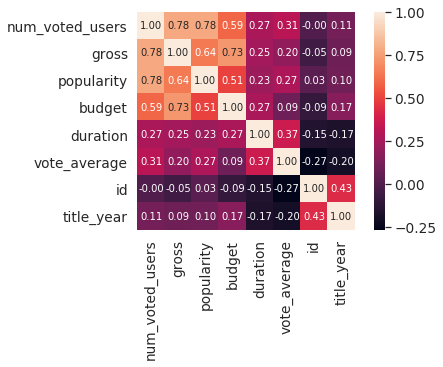
\includegraphics[height=10cm]{./contenido/imagenes/output_83_0.png}
\end{figure}

    { \hspace*{\fill} \\}
    
    Se usará este hallazgo para completar los valores faltantes de las
variables \textbf{gross} y \textbf{num\_voted\_users}. Para ello, se
realizarán regresiones en parejas de variables correlacionadas:

    \begin{tcolorbox}[breakable, size=fbox, boxrule=1pt, pad at break*=1mm,colback=cellbackground, colframe=cellborder]
\prompt{In}{incolor}{61}{\hspace{4pt}}
\begin{Verbatim}[commandchars=\\\{\}]
\PY{n}{sns}\PY{o}{.}\PY{n}{set}\PY{p}{(}\PY{n}{font\PYZus{}scale}\PY{o}{=}\PY{l+m+mf}{1.25}\PY{p}{)}
\PY{c+c1}{\PYZsh{}cols = [\PYZsq{}gross\PYZsq{}, \PYZsq{}num\PYZus{}voted\PYZus{}users\PYZsq{}, \PYZsq{}num\PYZus{}critic\PYZus{}for\PYZus{}reviews\PYZsq{}, \PYZsq{}num\PYZus{}user\PYZus{}for\PYZus{}reviews\PYZsq{}]}
\PY{n}{cols} \PY{o}{=} \PY{p}{[}\PY{l+s+s1}{\PYZsq{}}\PY{l+s+s1}{gross}\PY{l+s+s1}{\PYZsq{}}\PY{p}{,} \PY{l+s+s1}{\PYZsq{}}\PY{l+s+s1}{num\PYZus{}voted\PYZus{}users}\PY{l+s+s1}{\PYZsq{}}\PY{p}{]}
\PY{n}{sns}\PY{o}{.}\PY{n}{pairplot}\PY{p}{(}\PY{n}{df\PYZus{}filling}\PY{o}{.}\PY{n}{dropna}\PY{p}{(}\PY{n}{how}\PY{o}{=}\PY{l+s+s1}{\PYZsq{}}\PY{l+s+s1}{any}\PY{l+s+s1}{\PYZsq{}}\PY{p}{)}\PY{p}{[}\PY{n}{cols}\PY{p}{]}\PY{p}{,}\PY{n}{diag\PYZus{}kind}\PY{o}{=}\PY{l+s+s1}{\PYZsq{}}\PY{l+s+s1}{kde}\PY{l+s+s1}{\PYZsq{}}\PY{p}{,} \PY{n}{size} \PY{o}{=} \PY{l+m+mf}{2.5}\PY{p}{)}
\PY{n}{plt}\PY{o}{.}\PY{n}{show}\PY{p}{(}\PY{p}{)}\PY{p}{;}
\end{Verbatim}
\end{tcolorbox}
\begin{figure}[h]
    \centering
    \captionsetup{width=10cm}
    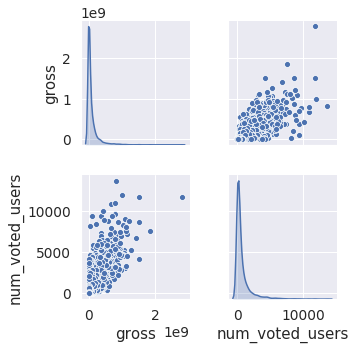
\includegraphics[height=10cm]{./contenido/imagenes/output_85_0.png}
\end{figure}

    { \hspace*{\fill} \\}
    
    En primer lugar, definimos una función que imputa los vbalores faltantes
mediante un ajuste lineal de los datos:

    \begin{tcolorbox}[breakable, size=fbox, boxrule=1pt, pad at break*=1mm,colback=cellbackground, colframe=cellborder]
\prompt{In}{incolor}{64}{\hspace{4pt}}
\begin{Verbatim}[commandchars=\\\{\}]
\PY{k}{def} \PY{n+nf}{variable\PYZus{}linreg\PYZus{}imputation}\PY{p}{(}\PY{n}{df}\PY{p}{,} \PY{n}{col\PYZus{}to\PYZus{}predict}\PY{p}{,} \PY{n}{ref\PYZus{}col}\PY{p}{)}\PY{p}{:}
    \PY{l+s+sd}{\PYZdq{}\PYZdq{}\PYZdq{}Completa los valores de la variable col\PYZus{}to\PYZus{}predict haciendo una regresión}
\PY{l+s+sd}{    lineal en la que la variable predictora es ref\PYZus{}col}

\PY{l+s+sd}{    Arguments:}
\PY{l+s+sd}{        df \PYZhy{}\PYZhy{} DataFrame de películas}
\PY{l+s+sd}{        col\PYZus{}to\PYZus{}predict \PYZhy{}\PYZhy{} Variable a predecir}
\PY{l+s+sd}{        ref\PYZus{}col \PYZhy{}\PYZhy{} Variable con la que predecir}

\PY{l+s+sd}{    Returns:}
\PY{l+s+sd}{        df \PYZhy{}\PYZhy{} DataFrame de películas completado}
\PY{l+s+sd}{    \PYZdq{}\PYZdq{}\PYZdq{}}
    \PY{n}{regr} \PY{o}{=} \PY{n}{linear\PYZus{}model}\PY{o}{.}\PY{n}{LinearRegression}\PY{p}{(}\PY{p}{)}
    \PY{n}{test} \PY{o}{=} \PY{n}{df}\PY{p}{[}\PY{p}{[}\PY{n}{col\PYZus{}to\PYZus{}predict}\PY{p}{,}\PY{n}{ref\PYZus{}col}\PY{p}{]}\PY{p}{]}\PY{o}{.}\PY{n}{dropna}\PY{p}{(}\PY{n}{how}\PY{o}{=}\PY{l+s+s1}{\PYZsq{}}\PY{l+s+s1}{any}\PY{l+s+s1}{\PYZsq{}}\PY{p}{,} \PY{n}{axis} \PY{o}{=} \PY{l+m+mi}{0}\PY{p}{)}
    \PY{n}{X} \PY{o}{=} \PY{n}{np}\PY{o}{.}\PY{n}{array}\PY{p}{(}\PY{n}{test}\PY{p}{[}\PY{n}{ref\PYZus{}col}\PY{p}{]}\PY{p}{)}
    \PY{n}{Y} \PY{o}{=} \PY{n}{np}\PY{o}{.}\PY{n}{array}\PY{p}{(}\PY{n}{test}\PY{p}{[}\PY{n}{col\PYZus{}to\PYZus{}predict}\PY{p}{]}\PY{p}{)}
    \PY{n}{X} \PY{o}{=} \PY{n}{X}\PY{o}{.}\PY{n}{reshape}\PY{p}{(}\PY{n+nb}{len}\PY{p}{(}\PY{n}{X}\PY{p}{)}\PY{p}{,}\PY{l+m+mi}{1}\PY{p}{)}
    \PY{n}{Y} \PY{o}{=} \PY{n}{Y}\PY{o}{.}\PY{n}{reshape}\PY{p}{(}\PY{n+nb}{len}\PY{p}{(}\PY{n}{Y}\PY{p}{)}\PY{p}{,}\PY{l+m+mi}{1}\PY{p}{)}
    \PY{n}{regr}\PY{o}{.}\PY{n}{fit}\PY{p}{(}\PY{n}{X}\PY{p}{,} \PY{n}{Y}\PY{p}{)}

    \PY{n}{test} \PY{o}{=} \PY{n}{df}\PY{p}{[}\PY{n}{df}\PY{p}{[}\PY{n}{col\PYZus{}to\PYZus{}predict}\PY{p}{]}\PY{o}{.}\PY{n}{isnull}\PY{p}{(}\PY{p}{)} \PY{o}{\PYZam{}} \PY{n}{df}\PY{p}{[}\PY{n}{ref\PYZus{}col}\PY{p}{]}\PY{o}{.}\PY{n}{notnull}\PY{p}{(}\PY{p}{)}\PY{p}{]}
    \PY{k}{for} \PY{n}{index}\PY{p}{,} \PY{n}{row} \PY{o+ow}{in} \PY{n}{test}\PY{o}{.}\PY{n}{iterrows}\PY{p}{(}\PY{p}{)}\PY{p}{:}
        \PY{n}{value} \PY{o}{=} \PY{n+nb}{float}\PY{p}{(}\PY{n}{regr}\PY{o}{.}\PY{n}{predict}\PY{p}{(}\PY{n}{row}\PY{p}{[}\PY{n}{ref\PYZus{}col}\PY{p}{]}\PY{p}{)}\PY{p}{)}
        \PY{n}{df}\PY{o}{.}\PY{n}{at}\PY{p}{[}\PY{n}{index}\PY{p}{,} \PY{n}{col\PYZus{}to\PYZus{}predict}\PY{p}{]} \PY{o}{=}  \PY{n}{value}
    \PY{k}{return} \PY{n}{df}
\end{Verbatim}
\end{tcolorbox}

    Esta función toma el dataframe como entrada y los nombres de dos
columnas. Se realiza un ajuste lineal entre estas dos columnas y se usa
para rellenar los datos faltantes de la primera columna dada:

    \begin{tcolorbox}[breakable, size=fbox, boxrule=1pt, pad at break*=1mm,colback=cellbackground, colframe=cellborder]
\prompt{In}{incolor}{65}{\hspace{4pt}}
\begin{Verbatim}[commandchars=\\\{\}]
\PY{n}{variable\PYZus{}linreg\PYZus{}imputation}\PY{p}{(}\PY{n}{df\PYZus{}filling}\PY{p}{,} \PY{l+s+s1}{\PYZsq{}}\PY{l+s+s1}{gross}\PY{l+s+s1}{\PYZsq{}}\PY{p}{,} \PY{l+s+s1}{\PYZsq{}}\PY{l+s+s1}{num\PYZus{}voted\PYZus{}users}\PY{l+s+s1}{\PYZsq{}}\PY{p}{)}
\end{Verbatim}
\end{tcolorbox}

            \begin{tcolorbox}[breakable, boxrule=.5pt, size=fbox, pad at break*=1mm, opacityfill=0]
\prompt{Out}{outcolor}{65}{\hspace{3.5pt}}
\begin{Verbatim}[commandchars=\\\{\}]
                                   movie\_title  title\_year  \textbackslash{}
0                                       Avatar      2009.0
1     Pirates of the Caribbean: At World's End      2007.0
2                                      Spectre      2015.0
3                        The Dark Knight Rises      2012.0
4                                  John Carter      2012.0
{\ldots}                                        {\ldots}         {\ldots}
4798                               El Mariachi      1992.0
4799                                 Newlyweds      2011.0
4800                 Signed, Sealed, Delivered      2013.0
4801                          Shanghai Calling      2012.0
4802                         My Date with Drew      2005.0

                                        genres  \textbackslash{}
0     Action|Adventure|Fantasy|Science Fiction
1                     Adventure|Fantasy|Action
2                       Action|Adventure|Crime
3                  Action|Crime|Drama|Thriller
4             Action|Adventure|Science Fiction
{\ldots}                                        {\ldots}
4798                     Action|Crime|Thriller
4799                            Comedy|Romance
4800             Comedy|Drama|Romance|TV Movie
4801
4802                               Documentary

                                          plot\_keywords      director\_name  \textbackslash{}
0     culture clash|future|space colony|society|spac{\ldots}      James Cameron
1     ocean|drug abuse|exotic island|east india trad{\ldots}     Gore Verbinski
2     spy|based on novel|secret agent|sequel|british{\ldots}         Sam Mendes
3     dc comics|crime fighter|terrorist|secret ident{\ldots}  Christopher Nolan
4     based on novel|mars|medallion|space travel|pri{\ldots}     Andrew Stanton
{\ldots}                                                 {\ldots}                {\ldots}
4798     united states–mexico barrier|stagecoach|weapon   Robert Rodriguez
4799                                                          Edward Burns
4800  date|love at first sight|narration|investigato{\ldots}        Scott Smith
4801                                                           Daniel Hsia
4802                          obsession|camcorder|crush   Brian Herzlinger

          actor\_1\_name      actor\_2\_name        actor\_3\_name  num\_voted\_users  \textbackslash{}
0          Zoe Saldana  Sigourney Weaver        Stephen Lang            11800
1        Orlando Bloom   Keira Knightley   Stellan Skarsgård             4500
2      Christoph Waltz       Léa Seydoux       Ralph Fiennes             4466
3        Michael Caine       Gary Oldman       Anne Hathaway             9106
4         Lynn Collins   Samantha Morton        Willem Dafoe             2124
{\ldots}                {\ldots}               {\ldots}                 {\ldots}              {\ldots}
4798    Jaime de Hoyos   Peter Marquardt     Reinol Martinez              238
4799       Kerry Bishé   Marsha Dietlein  Caitlin Fitzgerald                5
4800     Kristin Booth      Crystal Lowe     Geoff Gustafson                6
4801       Eliza Coupe       Bill Paxton           Alan Ruck                7
4802  Brian Herzlinger     Corey Feldman        Eric Roberts               16

      language                   country  vote\_average  duration       gross
0      English  United States of America           7.2     162.0  2787965087
1      English  United States of America           6.9     169.0   961000000
2     Français            United Kingdom           6.3     148.0   880674609
3      English  United States of America           7.6     165.0  1084939099
4      English  United States of America           6.1     132.0   284139100
{\ldots}        {\ldots}                       {\ldots}           {\ldots}       {\ldots}         {\ldots}
4798   Español                    Mexico           6.6      81.0     2040920
4799       NaN                       NaN           5.9      85.0           0
4800   English  United States of America           7.0     120.0           0
4801   English  United States of America           5.7      98.0           0
4802   English  United States of America           6.3      90.0           0

[4803 rows x 14 columns]
\end{Verbatim}
\end{tcolorbox}
        
    Por último, puede verse a cantidad de información faltante aun en el
dataframe:

    \begin{tcolorbox}[breakable, size=fbox, boxrule=1pt, pad at break*=1mm,colback=cellbackground, colframe=cellborder]
\prompt{In}{incolor}{66}{\hspace{4pt}}
\begin{Verbatim}[commandchars=\\\{\}]
\PY{n}{df} \PY{o}{=} \PY{n}{df\PYZus{}filling}\PY{o}{.}\PY{n}{copy}\PY{p}{(}\PY{n}{deep} \PY{o}{=} \PY{k+kc}{True}\PY{p}{)}
\PY{n}{missing\PYZus{}df} \PY{o}{=} \PY{n}{df}\PY{o}{.}\PY{n}{isnull}\PY{p}{(}\PY{p}{)}\PY{o}{.}\PY{n}{sum}\PY{p}{(}\PY{n}{axis}\PY{o}{=}\PY{l+m+mi}{0}\PY{p}{)}\PY{o}{.}\PY{n}{reset\PYZus{}index}\PY{p}{(}\PY{p}{)}
\PY{n}{missing\PYZus{}df}\PY{o}{.}\PY{n}{columns} \PY{o}{=} \PY{p}{[}\PY{l+s+s1}{\PYZsq{}}\PY{l+s+s1}{column\PYZus{}name}\PY{l+s+s1}{\PYZsq{}}\PY{p}{,} \PY{l+s+s1}{\PYZsq{}}\PY{l+s+s1}{missing\PYZus{}count}\PY{l+s+s1}{\PYZsq{}}\PY{p}{]}
\PY{n}{missing\PYZus{}df}\PY{p}{[}\PY{l+s+s1}{\PYZsq{}}\PY{l+s+s1}{filling\PYZus{}factor}\PY{l+s+s1}{\PYZsq{}}\PY{p}{]} \PY{o}{=} \PY{p}{(}\PY{n}{df}\PY{o}{.}\PY{n}{shape}\PY{p}{[}\PY{l+m+mi}{0}\PY{p}{]} 
                                \PY{o}{\PYZhy{}} \PY{n}{missing\PYZus{}df}\PY{p}{[}\PY{l+s+s1}{\PYZsq{}}\PY{l+s+s1}{missing\PYZus{}count}\PY{l+s+s1}{\PYZsq{}}\PY{p}{]}\PY{p}{)} \PY{o}{/} \PY{n}{df}\PY{o}{.}\PY{n}{shape}\PY{p}{[}\PY{l+m+mi}{0}\PY{p}{]} \PY{o}{*} \PY{l+m+mi}{100}
\PY{n}{missing\PYZus{}df} \PY{o}{=} \PY{n}{missing\PYZus{}df}\PY{o}{.}\PY{n}{sort\PYZus{}values}\PY{p}{(}\PY{l+s+s1}{\PYZsq{}}\PY{l+s+s1}{filling\PYZus{}factor}\PY{l+s+s1}{\PYZsq{}}\PY{p}{)}\PY{o}{.}\PY{n}{reset\PYZus{}index}\PY{p}{(}\PY{n}{drop} \PY{o}{=} \PY{k+kc}{True}\PY{p}{)}
\PY{n}{missing\PYZus{}df}
\end{Verbatim}
\end{tcolorbox}

            \begin{tcolorbox}[breakable, boxrule=.5pt, size=fbox, pad at break*=1mm, opacityfill=0]
\prompt{Out}{outcolor}{66}{\hspace{3.5pt}}
\begin{Verbatim}[commandchars=\\\{\}]
        column\_name  missing\_count  filling\_factor
0           country            174       96.377264
1      actor\_3\_name             93       98.063710
2          language             86       98.209452
3      actor\_2\_name             63       98.688320
4      actor\_1\_name             53       98.896523
5     director\_name             30       99.375390
6          duration              2       99.958359
7        title\_year              1       99.979180
8       movie\_title              0      100.000000
9            genres              0      100.000000
10    plot\_keywords              0      100.000000
11  num\_voted\_users              0      100.000000
12     vote\_average              0      100.000000
13            gross              0      100.000000
\end{Verbatim}
\end{tcolorbox}
        
    y puede verse que en el peor de los casos el la completitud está
alrededor del 96\%.

    \begin{tcolorbox}[breakable, size=fbox, boxrule=1pt, pad at break*=1mm,colback=cellbackground, colframe=cellborder]
\prompt{In}{incolor}{67}{\hspace{4pt}}
\begin{Verbatim}[commandchars=\\\{\}]
\PY{n}{df} \PY{o}{=} \PY{n}{df\PYZus{}filling}\PY{o}{.}\PY{n}{copy}\PY{p}{(}\PY{n}{deep}\PY{o}{=}\PY{k+kc}{True}\PY{p}{)}
\PY{n}{df}\PY{o}{.}\PY{n}{reset\PYZus{}index}\PY{p}{(}\PY{n}{inplace} \PY{o}{=} \PY{k+kc}{True}\PY{p}{,} \PY{n}{drop} \PY{o}{=} \PY{k+kc}{True}\PY{p}{)}
\end{Verbatim}
\end{tcolorbox}

    \begin{center}\rule{0.5\linewidth}{\linethickness}\end{center}

\subsection{3. MOTOR DE RECOMENDACIÓN}\label{motor-de-recomendaciuxf3n}

    \begin{center}\rule{0.5\linewidth}{\linethickness}\end{center}

\subsubsection{3.1 Funcionamiento básico del
motor}\label{funcionamiento-buxe1sico-del-motor}

El orden para construir el motor de recomendación tendrá dos pasos
básicos: 1. Elegir \(N\) películas con un contenido similar a la entrada
dada por el usuario 2. Seleccionar las 5 películas mas populares de
entre esas \(N\) películas

\paragraph{3.1.1 Similaridad}\label{similaridad}

Cuando se construye el motor, el primer paso consiste en definir un
criterio que pueda aportar información sobre cómo de parecidas son dos
películas. En primer lugar, tenemos en cuenta la descripción de la
película seleccionada por el usuario. De ahi tomamos el director, los
nombres de los actores y algunas keywords. A partir de estos datos,
creamos una matriz en la que cada fila se corresponde con una película
de la base de datos y en la que las columnas corresponden con lo dicho
anteriormente junto con los \emph{k} generos que se describieron en la
sección 1.4 When builing the engine, the first step thus consists in
defining a criteria that would tell us how close two films are. To do
so, I start from the description of the film that was selected by the
user: from it, I get the director name, the names of the actors and a
few keywords. I then build a matrix where each row corresponds to a film
of the database and where the columns correspond to the previous
quantities (director + actors + keywords) plus the \emph{k} genres that
were described in section 1.4:

    \begin{verbatim}
<th class="tg-g7sd">movie<br>title<br></th>
<th class="tg-g7sd">director</th>
<th class="tg-g7sd">actor 1<br></th>
<th class="tg-g7sd">a2</th>
<th class="tg-fymr">a3</th>
<th class="tg-fymr">keyword 1</th>
<th class="tg-fymr">k2</th>
<th class="tg-fymr">genre1</th>
<th class="tg-fymr">g2</th>
<th class="tg-fymr">...</th>
<th class="tg-fymr">gk</th>
\end{verbatim}

\begin{verbatim}
<td class="tg-lboi"><br>Film1</td>
<td class="tg-lboi">$a_{11}$</td>
<td class="tg-lboi">$a_{12}$</td>
<td class="tg-lboi"></td>
<td class="tg-0pky"></td>
<td class="tg-0pky">...</td>
<td class="tg-0pky"></td>
<td class="tg-0pky"></td>
<td class="tg-0pky"></td>
<td class="tg-0pky">...</td>
<td class="tg-0pky">$a_{1q}$</td>
\end{verbatim}

\begin{verbatim}
<td class="tg-lboi">...</td>
<td class="tg-lboi"></td>
<td class="tg-lboi"></td>
<td class="tg-lboi"></td>
<td class="tg-0pky"></td>
<td class="tg-0pky">...</td>
<td class="tg-0pky"></td>
<td class="tg-0pky"></td>
<td class="tg-0pky"></td>
<td class="tg-0pky">...</td>
<td class="tg-0pky"></td>
\end{verbatim}

\begin{verbatim}
<td class="tg-lboi">Film i </td>
<td class="tg-lboi">$a_{i1}$</td>
<td class="tg-lboi">$a_{i2}$</td>
<td class="tg-lboi"></td>
<td class="tg-0pky"></td>
<td class="tg-0pky">$a_{ij}$</td>
<td class="tg-0pky"></td>
<td class="tg-0pky"></td>
<td class="tg-0pky"></td>
<td class="tg-0pky">...</td>
<td class="tg-0pky">$a_{iq}$</td>
\end{verbatim}

\begin{verbatim}
<td class="tg-0pky">...</td>
<td class="tg-0pky"></td>
<td class="tg-0pky"></td>
<td class="tg-0pky"></td>
<td class="tg-0pky"></td>
<td class="tg-0pky">...</td>
<td class="tg-0pky"></td>
<td class="tg-0pky"></td>
<td class="tg-0pky"></td>
<td class="tg-0pky">...</td>
<td class="tg-0pky"></td>
\end{verbatim}

\begin{verbatim}
<td class="tg-0pky">Film p</td>
<td class="tg-0pky">$a_{p1}$</td>
<td class="tg-0pky">$a_{p2}$</td>
<td class="tg-0pky"></td>
<td class="tg-0pky"></td>
<td class="tg-0pky">...</td>
<td class="tg-0pky"></td>
<td class="tg-0pky"></td>
<td class="tg-0pky"></td>
<td class="tg-0pky">...</td>
<td class="tg-0pky">$a_{pq}$</td>
\end{verbatim}

    \begin{table}[]
\centering
\begin{tabular}{|l|l|l|l|l|l|l|l|l|l|l|}
\hline
\textbf{\begin{tabular}[c]{@{}l@{}}movie\\ title\end{tabular}} &
  \textbf{director} &
  \textbf{actor 1} &
  \textbf{a2} &
  \textbf{a3} &
  \textbf{keyword 1} &
  \textbf{k2} &
  \textbf{genre1} &
  \textbf{g2} &
  \textbf{...} &
  \textbf{gk} \\ \hline
Film1  & $a_{11}$ & $a_{12}$ &  &  & ...      &  &  &  & ... & $a_{1q}$ \\ \hline
...    &          &          &  &  & ...      &  &  &  & ... &          \\ \hline
Film i & $a_{i1}$ & $a_{i2}$ &  &  & $a_{ij}$ &  &  &  & ... & $a_{iq}$ \\ \hline
...    &          &          &  &  & ...      &  &  &  & ... &          \\ \hline
Film p & $a_{p1}$ & $a_{p2}$ &  &  & ...      &  &  &  & ... & $a_{pq}$ \\ \hline
\end{tabular}
\caption{Matriz generada para el cálculo de la similaridad entre dos películas}
\label{tab:similarity}
\end{table}

    En esta matriz, el elemento \(a_{ij}\) toma el valor 0 o 1 dependiendo
de la correspondencia entre la significancia entre la columna \(j\) y el
contenido de la película \(i\). Por ejemplo, si "keyword1" está en la
película \(i\), tendremos \(a_{ij} = 1\) y \(0\) en otro caso. Una vez
esta matriz se ha definido, determinamos la distnaica entre dos
películas mediante:

\begin{eqnarray}
d_{m, n} = \sqrt{  \sum_{i = 1}^{N} \left( a_{m,i}  - a_{n,i} \right)^2  } 
\end{eqnarray}

En este punto, únicamente tenemos que seleccionar las \(N\) películas
que son más cercanas a la entrada seleccionada por el usuario.

\paragraph{3.1.2 Popularidad}\label{popularidad}

Atendiendo a la similaridad entre películas, seleccionamos una lista de
\(N\) películas. En etse punto, seleccionaremos únicamente 5 películas.
Para ello, damos una puntuación a cada entrada. Se computa la puntuación
de acuerdo a estos tres criterios: - La puntuación en IMDB - El número
de votos recibidos por la película - El año de lanzamiento

Los dos primeros serán una medida directa de la popularidad de varias
entradas. Para el tercer criterio, se introduce el año de lanzamiento.
Se asume que las preferidas por la persona serán en la mayoria de los
casos de la misma época.

A continuación, calculamos la puntuación de acuerdo a esta ecuación:

    \begin{eqnarray}
\mathrm{score} = IMDB^2 \times \phi_{\sigma_1, c_1} \times  \phi_{\sigma_2, c_2},
\end{eqnarray}

donde \(\phi\) es una función gaussiana del tipo

\begin{eqnarray}
\phi_{\sigma, c}(x) \propto \mathrm{exp}\left(-\frac{(x-c)^2}{2 \, \sigma^2}\right).
\end{eqnarray}

    Para lo votos, tomamos el máximo número de votos entre las \(N\)
películas y fijamos \(\sigma_1 = c_1 = m\). Para lso años, ponemos
\(\sigma_1 = 20\) y centramos la gaussiana en el año de la película
seleccionada por el usuario. Con las gaussianas, se pone más peso en las
entradas con mayor número de votos y en las que el año de salida es
cercano al de la película seleccionada por el usuario.

    \begin{center}\rule{0.5\linewidth}{\linethickness}\end{center}

\subsubsection{3.2 Definición de las funciones del
motor}\label{definiciuxf3n-de-las-funciones-del-motor}

    \begin{tcolorbox}[breakable, size=fbox, boxrule=1pt, pad at break*=1mm,colback=cellbackground, colframe=cellborder]
\prompt{In}{incolor}{68}{\hspace{4pt}}
\begin{Verbatim}[commandchars=\\\{\}]
\PY{n}{gaussian\PYZus{}filter} \PY{o}{=} \PY{k}{lambda} \PY{n}{x}\PY{p}{,}\PY{n}{y}\PY{p}{,}\PY{n}{sigma}\PY{p}{:} \PY{n}{math}\PY{o}{.}\PY{n}{exp}\PY{p}{(}\PY{o}{\PYZhy{}}\PY{p}{(}\PY{n}{x}\PY{o}{\PYZhy{}}\PY{n}{y}\PY{p}{)}\PY{o}{*}\PY{o}{*}\PY{l+m+mi}{2}\PY{o}{/}\PY{p}{(}\PY{l+m+mi}{2}\PY{o}{*}\PY{n}{sigma}\PY{o}{*}\PY{o}{*}\PY{l+m+mi}{2}\PY{p}{)}\PY{p}{)}
\end{Verbatim}
\end{tcolorbox}

    \begin{tcolorbox}[breakable, size=fbox, boxrule=1pt, pad at break*=1mm,colback=cellbackground, colframe=cellborder]
\prompt{In}{incolor}{69}{\hspace{4pt}}
\begin{Verbatim}[commandchars=\\\{\}]
\PY{k}{def} \PY{n+nf}{entry\PYZus{}variables}\PY{p}{(}\PY{n}{df}\PY{p}{,} \PY{n}{id\PYZus{}entry}\PY{p}{)}\PY{p}{:} 
    \PY{l+s+sd}{\PYZdq{}\PYZdq{}\PYZdq{}Calcula los valores tomados por las variables director\PYZus{}name, actor\PYZus{}[1,2,3]\PYZus{}name y plot\PYZus{}keywords para la}
\PY{l+s+sd}{    película seleccionada por el usuario.}
\PY{l+s+sd}{    }
\PY{l+s+sd}{    Arguments:}
\PY{l+s+sd}{        df \PYZhy{}\PYZhy{} DataFrame de películas}
\PY{l+s+sd}{        id\PYZus{}entry \PYZhy{}\PYZhy{} Id de la entrada seleccionada}
\PY{l+s+sd}{    }
\PY{l+s+sd}{    Returns:}
\PY{l+s+sd}{        col\PYZus{}labels \PYZhy{}\PYZhy{} Lista que contiene los valores extraidos para la película seleccionada}
\PY{l+s+sd}{    \PYZdq{}\PYZdq{}\PYZdq{}}
    
    \PY{n}{col\PYZus{}labels} \PY{o}{=} \PY{p}{[}\PY{p}{]}    
    \PY{k}{if} \PY{n}{pd}\PY{o}{.}\PY{n}{notnull}\PY{p}{(}\PY{n}{df}\PY{p}{[}\PY{l+s+s1}{\PYZsq{}}\PY{l+s+s1}{director\PYZus{}name}\PY{l+s+s1}{\PYZsq{}}\PY{p}{]}\PY{o}{.}\PY{n}{iloc}\PY{p}{[}\PY{n}{id\PYZus{}entry}\PY{p}{]}\PY{p}{)}\PY{p}{:}
        \PY{k}{for} \PY{n}{s} \PY{o+ow}{in} \PY{n}{df}\PY{p}{[}\PY{l+s+s1}{\PYZsq{}}\PY{l+s+s1}{director\PYZus{}name}\PY{l+s+s1}{\PYZsq{}}\PY{p}{]}\PY{o}{.}\PY{n}{iloc}\PY{p}{[}\PY{n}{id\PYZus{}entry}\PY{p}{]}\PY{o}{.}\PY{n}{split}\PY{p}{(}\PY{l+s+s1}{\PYZsq{}}\PY{l+s+s1}{|}\PY{l+s+s1}{\PYZsq{}}\PY{p}{)}\PY{p}{:}
            \PY{n}{col\PYZus{}labels}\PY{o}{.}\PY{n}{append}\PY{p}{(}\PY{n}{s}\PY{p}{)}
            
    \PY{k}{for} \PY{n}{i} \PY{o+ow}{in} \PY{n+nb}{range}\PY{p}{(}\PY{l+m+mi}{3}\PY{p}{)}\PY{p}{:}
        \PY{n}{column} \PY{o}{=} \PY{l+s+s1}{\PYZsq{}}\PY{l+s+s1}{actor\PYZus{}NUM\PYZus{}name}\PY{l+s+s1}{\PYZsq{}}\PY{o}{.}\PY{n}{replace}\PY{p}{(}\PY{l+s+s1}{\PYZsq{}}\PY{l+s+s1}{NUM}\PY{l+s+s1}{\PYZsq{}}\PY{p}{,} \PY{n+nb}{str}\PY{p}{(}\PY{n}{i}\PY{o}{+}\PY{l+m+mi}{1}\PY{p}{)}\PY{p}{)}
        \PY{k}{if} \PY{n}{pd}\PY{o}{.}\PY{n}{notnull}\PY{p}{(}\PY{n}{df}\PY{p}{[}\PY{n}{column}\PY{p}{]}\PY{o}{.}\PY{n}{iloc}\PY{p}{[}\PY{n}{id\PYZus{}entry}\PY{p}{]}\PY{p}{)}\PY{p}{:}
            \PY{k}{for} \PY{n}{s} \PY{o+ow}{in} \PY{n}{df}\PY{p}{[}\PY{n}{column}\PY{p}{]}\PY{o}{.}\PY{n}{iloc}\PY{p}{[}\PY{n}{id\PYZus{}entry}\PY{p}{]}\PY{o}{.}\PY{n}{split}\PY{p}{(}\PY{l+s+s1}{\PYZsq{}}\PY{l+s+s1}{|}\PY{l+s+s1}{\PYZsq{}}\PY{p}{)}\PY{p}{:}
                \PY{n}{col\PYZus{}labels}\PY{o}{.}\PY{n}{append}\PY{p}{(}\PY{n}{s}\PY{p}{)}
                
    \PY{k}{if} \PY{n}{pd}\PY{o}{.}\PY{n}{notnull}\PY{p}{(}\PY{n}{df}\PY{p}{[}\PY{l+s+s1}{\PYZsq{}}\PY{l+s+s1}{plot\PYZus{}keywords}\PY{l+s+s1}{\PYZsq{}}\PY{p}{]}\PY{o}{.}\PY{n}{iloc}\PY{p}{[}\PY{n}{id\PYZus{}entry}\PY{p}{]}\PY{p}{)}\PY{p}{:}
        \PY{k}{for} \PY{n}{s} \PY{o+ow}{in} \PY{n}{df}\PY{p}{[}\PY{l+s+s1}{\PYZsq{}}\PY{l+s+s1}{plot\PYZus{}keywords}\PY{l+s+s1}{\PYZsq{}}\PY{p}{]}\PY{o}{.}\PY{n}{iloc}\PY{p}{[}\PY{n}{id\PYZus{}entry}\PY{p}{]}\PY{o}{.}\PY{n}{split}\PY{p}{(}\PY{l+s+s1}{\PYZsq{}}\PY{l+s+s1}{|}\PY{l+s+s1}{\PYZsq{}}\PY{p}{)}\PY{p}{:}
            \PY{n}{col\PYZus{}labels}\PY{o}{.}\PY{n}{append}\PY{p}{(}\PY{n}{s}\PY{p}{)}
    \PY{k}{return} \PY{n}{col\PYZus{}labels}
\end{Verbatim}
\end{tcolorbox}

    \begin{tcolorbox}[breakable, size=fbox, boxrule=1pt, pad at break*=1mm,colback=cellbackground, colframe=cellborder]
\prompt{In}{incolor}{70}{\hspace{4pt}}
\begin{Verbatim}[commandchars=\\\{\}]
\PY{n}{df}\PY{o}{.}\PY{n}{head}\PY{p}{(}\PY{l+m+mi}{2}\PY{p}{)}
\end{Verbatim}
\end{tcolorbox}

            \begin{tcolorbox}[breakable, boxrule=.5pt, size=fbox, pad at break*=1mm, opacityfill=0]
\prompt{Out}{outcolor}{70}{\hspace{3.5pt}}
\begin{Verbatim}[commandchars=\\\{\}]
                                movie\_title  title\_year  \textbackslash{}
0                                    Avatar      2009.0
1  Pirates of the Caribbean: At World's End      2007.0

                                     genres  \textbackslash{}
0  Action|Adventure|Fantasy|Science Fiction
1                  Adventure|Fantasy|Action

                                       plot\_keywords   director\_name  \textbackslash{}
0  culture clash|future|space colony|society|spac{\ldots}   James Cameron
1  ocean|drug abuse|exotic island|east india trad{\ldots}  Gore Verbinski

    actor\_1\_name      actor\_2\_name       actor\_3\_name  num\_voted\_users  \textbackslash{}
0    Zoe Saldana  Sigourney Weaver       Stephen Lang            11800
1  Orlando Bloom   Keira Knightley  Stellan Skarsgård             4500

  language                   country  vote\_average  duration       gross
0  English  United States of America           7.2     162.0  2787965087
1  English  United States of America           6.9     169.0   961000000
\end{Verbatim}
\end{tcolorbox}
        
    \begin{tcolorbox}[breakable, size=fbox, boxrule=1pt, pad at break*=1mm,colback=cellbackground, colframe=cellborder]
\prompt{In}{incolor}{71}{\hspace{4pt}}
\begin{Verbatim}[commandchars=\\\{\}]
\PY{k}{def} \PY{n+nf}{add\PYZus{}variables}\PY{p}{(}\PY{n}{df}\PY{p}{,} \PY{n}{REF\PYZus{}VAR}\PY{p}{)}\PY{p}{:}
    \PY{l+s+sd}{\PYZdq{}\PYZdq{}\PYZdq{}Añade al dataframe de películas las columnas dadas en REF\PYZus{}VAR (que serán el director, etc de una}
\PY{l+s+sd}{    película) y las inicializa a 0 o 1 dependiendo de si la película es del mismo director, tiene a ese actor}
\PY{l+s+sd}{    , etc}
\PY{l+s+sd}{    }
\PY{l+s+sd}{    Arguments:}
\PY{l+s+sd}{        df \PYZhy{}\PYZhy{} dataframe de películas}
\PY{l+s+sd}{        REF\PYZus{}VAR \PYZhy{}\PYZhy{} salida de aplicar entry\PYZus{}variables sobre el df y una película}
\PY{l+s+sd}{    }
\PY{l+s+sd}{    Returns:}
\PY{l+s+sd}{        df \PYZhy{}\PYZhy{} DataFrame con las nuevas películas}
\PY{l+s+sd}{    \PYZdq{}\PYZdq{}\PYZdq{}}
    \PY{k}{for} \PY{n}{s} \PY{o+ow}{in} \PY{n}{REF\PYZus{}VAR}\PY{p}{:} 
        \PY{n}{df}\PY{p}{[}\PY{n}{s}\PY{p}{]} \PY{o}{=} \PY{n}{pd}\PY{o}{.}\PY{n}{Series}\PY{p}{(}\PY{p}{[}\PY{l+m+mi}{0} \PY{k}{for} \PY{n}{\PYZus{}} \PY{o+ow}{in} \PY{n+nb}{range}\PY{p}{(}\PY{n+nb}{len}\PY{p}{(}\PY{n}{df}\PY{p}{)}\PY{p}{)}\PY{p}{]}\PY{p}{)}
    \PY{n}{columns} \PY{o}{=} \PY{p}{[}\PY{l+s+s1}{\PYZsq{}}\PY{l+s+s1}{genres}\PY{l+s+s1}{\PYZsq{}}\PY{p}{,} \PY{l+s+s1}{\PYZsq{}}\PY{l+s+s1}{actor\PYZus{}1\PYZus{}name}\PY{l+s+s1}{\PYZsq{}}\PY{p}{,} \PY{l+s+s1}{\PYZsq{}}\PY{l+s+s1}{actor\PYZus{}2\PYZus{}name}\PY{l+s+s1}{\PYZsq{}}\PY{p}{,}
                \PY{l+s+s1}{\PYZsq{}}\PY{l+s+s1}{actor\PYZus{}3\PYZus{}name}\PY{l+s+s1}{\PYZsq{}}\PY{p}{,} \PY{l+s+s1}{\PYZsq{}}\PY{l+s+s1}{director\PYZus{}name}\PY{l+s+s1}{\PYZsq{}}\PY{p}{,} \PY{l+s+s1}{\PYZsq{}}\PY{l+s+s1}{plot\PYZus{}keywords}\PY{l+s+s1}{\PYZsq{}}\PY{p}{]}
    \PY{k}{for} \PY{n}{category} \PY{o+ow}{in} \PY{n}{columns}\PY{p}{:}
        \PY{k}{for} \PY{n}{index}\PY{p}{,} \PY{n}{row} \PY{o+ow}{in} \PY{n}{df}\PY{o}{.}\PY{n}{iterrows}\PY{p}{(}\PY{p}{)}\PY{p}{:}
            \PY{k}{if} \PY{n}{pd}\PY{o}{.}\PY{n}{isnull}\PY{p}{(}\PY{n}{row}\PY{p}{[}\PY{n}{category}\PY{p}{]}\PY{p}{)}\PY{p}{:} 
                \PY{k}{continue}
            \PY{k}{for} \PY{n}{s} \PY{o+ow}{in} \PY{n}{row}\PY{p}{[}\PY{n}{category}\PY{p}{]}\PY{o}{.}\PY{n}{split}\PY{p}{(}\PY{l+s+s1}{\PYZsq{}}\PY{l+s+s1}{|}\PY{l+s+s1}{\PYZsq{}}\PY{p}{)}\PY{p}{:}
                \PY{k}{if} \PY{n}{s} \PY{o+ow}{in} \PY{n}{REF\PYZus{}VAR}\PY{p}{:} \PY{n}{df}\PY{o}{.}\PY{n}{set\PYZus{}value}\PY{p}{(}\PY{n}{index}\PY{p}{,} \PY{n}{s}\PY{p}{,} \PY{l+m+mi}{1}\PY{p}{)}            
    \PY{k}{return} \PY{n}{df}
\end{Verbatim}
\end{tcolorbox}

    \textbf{Function creating a list of films}: the \emph{recommand()}
function create a list of N (= 31) films similar to the film selected by
the user.

    \begin{tcolorbox}[breakable, size=fbox, boxrule=1pt, pad at break*=1mm,colback=cellbackground, colframe=cellborder]
\prompt{In}{incolor}{72}{\hspace{4pt}}
\begin{Verbatim}[commandchars=\\\{\}]
\PY{k}{def} \PY{n+nf}{recommend}\PY{p}{(}\PY{n}{df}\PY{p}{,} \PY{n}{id\PYZus{}entry}\PY{p}{,} \PY{n}{N} \PY{o}{=} \PY{l+m+mi}{31}\PY{p}{)}\PY{p}{:}
    \PY{l+s+sd}{\PYZdq{}\PYZdq{}\PYZdq{}}
\PY{l+s+sd}{    Crea una lista de N películas similares a las seleccionadas por el usuario}
\PY{l+s+sd}{    Arguments:}
\PY{l+s+sd}{        df \PYZhy{}\PYZhy{} DataFrame de películas}
\PY{l+s+sd}{        id\PYZus{}entry \PYZhy{}\PYZhy{} Id de la entrada seleccionada}
\PY{l+s+sd}{        N \PYZhy{}\PYZhy{} Number of films recommended (take into account that the nearest will be always itself)}
\PY{l+s+sd}{    }
\PY{l+s+sd}{    Returns:}
\PY{l+s+sd}{        list \PYZhy{}\PYZhy{} lista con los id de las películas recomendadas}
\PY{l+s+sd}{    \PYZdq{}\PYZdq{}\PYZdq{}}
    \PY{n}{df\PYZus{}copy} \PY{o}{=} \PY{n}{df}\PY{o}{.}\PY{n}{copy}\PY{p}{(}\PY{n}{deep} \PY{o}{=} \PY{k+kc}{True}\PY{p}{)}    
    \PY{n}{list\PYZus{}genres} \PY{o}{=} \PY{n+nb}{set}\PY{p}{(}\PY{p}{)}
    \PY{k}{for} \PY{n}{s} \PY{o+ow}{in} \PY{n}{df}\PY{p}{[}\PY{l+s+s1}{\PYZsq{}}\PY{l+s+s1}{genres}\PY{l+s+s1}{\PYZsq{}}\PY{p}{]}\PY{o}{.}\PY{n}{str}\PY{o}{.}\PY{n}{split}\PY{p}{(}\PY{l+s+s1}{\PYZsq{}}\PY{l+s+s1}{|}\PY{l+s+s1}{\PYZsq{}}\PY{p}{)}\PY{o}{.}\PY{n}{values}\PY{p}{:}
        \PY{n}{list\PYZus{}genres} \PY{o}{=} \PY{n}{list\PYZus{}genres}\PY{o}{.}\PY{n}{union}\PY{p}{(}\PY{n+nb}{set}\PY{p}{(}\PY{n}{s}\PY{p}{)}\PY{p}{)}    
    \PY{c+c1}{\PYZsh{}\PYZus{}\PYZus{}\PYZus{}\PYZus{}\PYZus{}\PYZus{}\PYZus{}\PYZus{}\PYZus{}\PYZus{}\PYZus{}\PYZus{}\PYZus{}\PYZus{}\PYZus{}\PYZus{}\PYZus{}\PYZus{}\PYZus{}\PYZus{}\PYZus{}\PYZus{}\PYZus{}\PYZus{}\PYZus{}\PYZus{}\PYZus{}\PYZus{}\PYZus{}\PYZus{}\PYZus{}\PYZus{}\PYZus{}\PYZus{}\PYZus{}\PYZus{}\PYZus{}\PYZus{}\PYZus{}\PYZus{}\PYZus{}\PYZus{}\PYZus{}\PYZus{}\PYZus{}\PYZus{}\PYZus{}\PYZus{}\PYZus{}\PYZus{}\PYZus{}\PYZus{}\PYZus{}}
    \PY{c+c1}{\PYZsh{} Creación de variables adicionales para comprobar la similaridad}
    \PY{n}{variables} \PY{o}{=} \PY{n}{entry\PYZus{}variables}\PY{p}{(}\PY{n}{df\PYZus{}copy}\PY{p}{,} \PY{n}{id\PYZus{}entry}\PY{p}{)}
    \PY{n}{variables} \PY{o}{+}\PY{o}{=} \PY{n+nb}{list}\PY{p}{(}\PY{n}{list\PYZus{}genres}\PY{p}{)}
    \PY{n}{df\PYZus{}new} \PY{o}{=} \PY{n}{add\PYZus{}variables}\PY{p}{(}\PY{n}{df\PYZus{}copy}\PY{p}{,} \PY{n}{variables}\PY{p}{)}
    \PY{c+c1}{\PYZsh{}\PYZus{}\PYZus{}\PYZus{}\PYZus{}\PYZus{}\PYZus{}\PYZus{}\PYZus{}\PYZus{}\PYZus{}\PYZus{}\PYZus{}\PYZus{}\PYZus{}\PYZus{}\PYZus{}\PYZus{}\PYZus{}\PYZus{}\PYZus{}\PYZus{}\PYZus{}\PYZus{}\PYZus{}\PYZus{}\PYZus{}\PYZus{}\PYZus{}\PYZus{}\PYZus{}\PYZus{}\PYZus{}\PYZus{}\PYZus{}\PYZus{}\PYZus{}\PYZus{}\PYZus{}\PYZus{}\PYZus{}\PYZus{}\PYZus{}\PYZus{}\PYZus{}\PYZus{}\PYZus{}\PYZus{}\PYZus{}\PYZus{}\PYZus{}\PYZus{}\PYZus{}\PYZus{}\PYZus{}\PYZus{}\PYZus{}\PYZus{}\PYZus{}\PYZus{}\PYZus{}\PYZus{}\PYZus{}\PYZus{}\PYZus{}\PYZus{}\PYZus{}\PYZus{}\PYZus{}\PYZus{}\PYZus{}\PYZus{}\PYZus{}\PYZus{}\PYZus{}\PYZus{}\PYZus{}\PYZus{}\PYZus{}\PYZus{}\PYZus{}\PYZus{}\PYZus{}\PYZus{}\PYZus{}}
    \PY{c+c1}{\PYZsh{} Determinación de los vecinos más próximos: la distancia se calcula con las nuevas vairables}
    \PY{n}{X} \PY{o}{=} \PY{n}{df\PYZus{}new}\PY{o}{.}\PY{n}{as\PYZus{}matrix}\PY{p}{(}\PY{n}{variables}\PY{p}{)}
    \PY{n}{nbrs} \PY{o}{=} \PY{n}{NearestNeighbors}\PY{p}{(}\PY{n}{n\PYZus{}neighbors}\PY{o}{=}\PY{n}{N}\PY{p}{,} \PY{n}{algorithm}\PY{o}{=}\PY{l+s+s1}{\PYZsq{}}\PY{l+s+s1}{auto}\PY{l+s+s1}{\PYZsq{}}\PY{p}{,} \PY{n}{metric}\PY{o}{=}\PY{l+s+s1}{\PYZsq{}}\PY{l+s+s1}{euclidean}\PY{l+s+s1}{\PYZsq{}}\PY{p}{)}\PY{o}{.}\PY{n}{fit}\PY{p}{(}\PY{n}{X}\PY{p}{)}

    \PY{n}{distances}\PY{p}{,} \PY{n}{indices} \PY{o}{=} \PY{n}{nbrs}\PY{o}{.}\PY{n}{kneighbors}\PY{p}{(}\PY{n}{X}\PY{p}{)}    
    \PY{n}{xtest} \PY{o}{=} \PY{n}{df\PYZus{}new}\PY{o}{.}\PY{n}{iloc}\PY{p}{[}\PY{n}{id\PYZus{}entry}\PY{p}{]}\PY{o}{.}\PY{n}{as\PYZus{}matrix}\PY{p}{(}\PY{n}{variables}\PY{p}{)}
    \PY{n}{xtest} \PY{o}{=} \PY{n}{xtest}\PY{o}{.}\PY{n}{reshape}\PY{p}{(}\PY{l+m+mi}{1}\PY{p}{,} \PY{o}{\PYZhy{}}\PY{l+m+mi}{1}\PY{p}{)}

    \PY{n}{distances}\PY{p}{,} \PY{n}{indices} \PY{o}{=} \PY{n}{nbrs}\PY{o}{.}\PY{n}{kneighbors}\PY{p}{(}\PY{n}{xtest}\PY{p}{)}

    \PY{k}{return} \PY{n}{indices}\PY{p}{[}\PY{l+m+mi}{0}\PY{p}{]}\PY{p}{[}\PY{p}{:}\PY{p}{]}
    
\end{Verbatim}
\end{tcolorbox}

    \begin{tcolorbox}[breakable, size=fbox, boxrule=1pt, pad at break*=1mm,colback=cellbackground, colframe=cellborder]
\prompt{In}{incolor}{73}{\hspace{4pt}}
\begin{Verbatim}[commandchars=\\\{\}]
\PY{n}{recommend}\PY{p}{(}\PY{n}{df}\PY{p}{,} \PY{l+m+mi}{2}\PY{p}{)}
\end{Verbatim}
\end{tcolorbox}

            \begin{tcolorbox}[breakable, boxrule=.5pt, size=fbox, pad at break*=1mm, opacityfill=0]
\prompt{Out}{outcolor}{73}{\hspace{3.5pt}}
\begin{Verbatim}[commandchars=\\\{\}]
array([   2,   29,   11, 1234, 1740, 1100,  640,  425, 2675, 1077,   62,
        134,  183, 3336,  469, 1343, 4339, 1542, 3494, 2433, 1615, 2644,
       2444, 1720, 1610, 1586, 3799, 1743, 1713, 4071, 1697])
\end{Verbatim}
\end{tcolorbox}
        
    \textbf{Function extracting some parameters from a list of films}: the
\emph{create\_film\_selection()} function extracts some variables of the
dataframe given in input and returns this list for a selection of N
films. This list is ordered according to criteria established in the
\emph{critere\_selection()} function.

    \begin{tcolorbox}[breakable, size=fbox, boxrule=1pt, pad at break*=1mm,colback=cellbackground, colframe=cellborder]
\prompt{In}{incolor}{74}{\hspace{4pt}}
\begin{Verbatim}[commandchars=\\\{\}]
\PY{k}{def} \PY{n+nf}{extract\PYZus{}parameters}\PY{p}{(}\PY{n}{df}\PY{p}{,} \PY{n}{list\PYZus{}films}\PY{p}{,} \PY{n}{N} \PY{o}{=} \PY{l+m+mi}{31}\PY{p}{)}\PY{p}{:}
    \PY{l+s+sd}{\PYZdq{}\PYZdq{}\PYZdq{}}
\PY{l+s+sd}{    Extrae algunas variables del dataframe dado como entrada y devuelve la lista de N películas.}
\PY{l+s+sd}{    Esta lista se ordena de acuerdo al criterio de la función selection\PYZus{}criteria}

\PY{l+s+sd}{    Arguments:}
\PY{l+s+sd}{        df \PYZhy{}\PYZhy{} DataFrame de películas}
\PY{l+s+sd}{        list\PYZus{}films \PYZhy{}\PYZhy{} Lista con las n películas recomendadas.}
\PY{l+s+sd}{    }
\PY{l+s+sd}{    Returns:}
\PY{l+s+sd}{        list \PYZhy{}\PYZhy{} lista con las variables relevantes para la ordenación, ordenadas por puntuación.}
\PY{l+s+sd}{    \PYZdq{}\PYZdq{}\PYZdq{}}
    \PY{n}{parametres\PYZus{}films} \PY{o}{=} \PY{p}{[}\PY{l+s+s1}{\PYZsq{}}\PY{l+s+s1}{\PYZus{}}\PY{l+s+s1}{\PYZsq{}} \PY{k}{for} \PY{n}{\PYZus{}} \PY{o+ow}{in} \PY{n+nb}{range}\PY{p}{(}\PY{n}{N}\PY{p}{)}\PY{p}{]}
    \PY{n}{i} \PY{o}{=} \PY{l+m+mi}{0}
    \PY{n}{max\PYZus{}users} \PY{o}{=} \PY{o}{\PYZhy{}}\PY{l+m+mi}{1}
    \PY{k}{for} \PY{n}{index} \PY{o+ow}{in} \PY{n}{list\PYZus{}films}\PY{p}{:}
        \PY{n}{parametres\PYZus{}films}\PY{p}{[}\PY{n}{i}\PY{p}{]} \PY{o}{=} \PY{n+nb}{list}\PY{p}{(}\PY{n}{df}\PY{o}{.}\PY{n}{iloc}\PY{p}{[}\PY{n}{index}\PY{p}{]}\PY{p}{[}\PY{p}{[}\PY{l+s+s1}{\PYZsq{}}\PY{l+s+s1}{movie\PYZus{}title}\PY{l+s+s1}{\PYZsq{}}\PY{p}{,} \PY{l+s+s1}{\PYZsq{}}\PY{l+s+s1}{title\PYZus{}year}\PY{l+s+s1}{\PYZsq{}}\PY{p}{,}
                                        \PY{l+s+s1}{\PYZsq{}}\PY{l+s+s1}{vote\PYZus{}average}\PY{l+s+s1}{\PYZsq{}}\PY{p}{,} 
                                        \PY{l+s+s1}{\PYZsq{}}\PY{l+s+s1}{num\PYZus{}voted\PYZus{}users}\PY{l+s+s1}{\PYZsq{}}\PY{p}{]}\PY{p}{]}\PY{p}{)}
        \PY{n}{parametres\PYZus{}films}\PY{p}{[}\PY{n}{i}\PY{p}{]}\PY{o}{.}\PY{n}{append}\PY{p}{(}\PY{n}{index}\PY{p}{)}
        \PY{n}{max\PYZus{}users} \PY{o}{=} \PY{n+nb}{max}\PY{p}{(}\PY{n}{max\PYZus{}users}\PY{p}{,} \PY{n}{parametres\PYZus{}films}\PY{p}{[}\PY{n}{i}\PY{p}{]}\PY{p}{[}\PY{l+m+mi}{4}\PY{p}{]} \PY{p}{)}
        \PY{n}{i} \PY{o}{+}\PY{o}{=} \PY{l+m+mi}{1}
    \PY{c+c1}{\PYZsh{} The first element is the selected film itself}
    \PY{n}{title\PYZus{}main} \PY{o}{=} \PY{n}{parametres\PYZus{}films}\PY{p}{[}\PY{l+m+mi}{0}\PY{p}{]}\PY{p}{[}\PY{l+m+mi}{0}\PY{p}{]}
    \PY{n}{ref\PYZus{}year}  \PY{o}{=} \PY{n}{parametres\PYZus{}films}\PY{p}{[}\PY{l+m+mi}{0}\PY{p}{]}\PY{p}{[}\PY{l+m+mi}{1}\PY{p}{]}
    \PY{n}{parametres\PYZus{}films}\PY{o}{.}\PY{n}{sort}\PY{p}{(}\PY{n}{key} \PY{o}{=} \PY{k}{lambda} \PY{n}{x}\PY{p}{:}\PY{n}{selection\PYZus{}criteria}\PY{p}{(}\PY{n}{title\PYZus{}main}\PY{p}{,} \PY{n}{max\PYZus{}users}\PY{p}{,}
                                                            \PY{n}{ref\PYZus{}year}\PY{p}{,} 
                                                            \PY{n}{title} \PY{o}{=} \PY{n}{x}\PY{p}{[}\PY{l+m+mi}{0}\PY{p}{]}\PY{p}{,} 
                                                            \PY{n}{year} \PY{o}{=} \PY{n}{x}\PY{p}{[}\PY{l+m+mi}{1}\PY{p}{]}\PY{p}{,}
                                                            \PY{n}{score} \PY{o}{=} \PY{n}{x}\PY{p}{[}\PY{l+m+mi}{2}\PY{p}{]}\PY{p}{,} 
                                                            \PY{n}{votes} \PY{o}{=} \PY{n}{x}\PY{p}{[}\PY{l+m+mi}{3}\PY{p}{]}\PY{p}{)}\PY{p}{,} \PY{n}{reverse} \PY{o}{=} \PY{k+kc}{True}\PY{p}{)}
    
    \PY{k}{return} \PY{n}{parametres\PYZus{}films} 
\end{Verbatim}
\end{tcolorbox}

    \textbf{Function comparing 2 film titles}: the sequel \emph{sequel()}
function compares the 2 titles passed in input and defines if these
titles are similar or not.

    \begin{tcolorbox}[breakable, size=fbox, boxrule=1pt, pad at break*=1mm,colback=cellbackground, colframe=cellborder]
\prompt{In}{incolor}{75}{\hspace{4pt}}
\begin{Verbatim}[commandchars=\\\{\}]
\PY{k}{def} \PY{n+nf}{sequel}\PY{p}{(}\PY{n}{title\PYZus{}1}\PY{p}{,} \PY{n}{title\PYZus{}2}\PY{p}{)}\PY{p}{:}   
    \PY{l+s+sd}{\PYZdq{}\PYZdq{}\PYZdq{}}
\PY{l+s+sd}{    Compara los títulos de dos películas y devuelve si son similares o no}
\PY{l+s+sd}{    }
\PY{l+s+sd}{    Arguments:}onf
\PY{l+s+sd}{        title\PYZus{}1 \PYZhy{}\PYZhy{} String con el primer título}
\PY{l+s+sd}{        title\PYZus{}2 \PYZhy{}\PYZhy{} String con el segundo título}
\PY{l+s+sd}{    }
\PY{l+s+sd}{    Returns:}
\PY{l+s+sd}{        list \PYZhy{}\PYZhy{} lista con las variables relevantes para la ordenación, ordenadas por puntuación.}
\PY{l+s+sd}{    \PYZdq{}\PYZdq{}\PYZdq{}}
    \PY{c+c1}{\PYZsh{}print(\PYZdq{}\PYZdl{}\PYZdl{}\PYZdl{}\PYZdl{}\PYZdl{}\PYZdl{}\PYZdl{}\PYZdl{}\PYZdl{}\PYZdl{}\PYZdl{}\PYZdl{}\PYZdl{}\PYZdl{}\PYZdl{}\PYZdl{}\PYZdl{}\PYZdl{}\PYZdl{}\PYZdl{}\PYZdl{}\PYZdl{}\PYZdq{})}
    \PY{c+c1}{\PYZsh{}print(title\PYZus{}1, \PYZdq{}|\PYZdq{},title\PYZus{}2)}
    \PY{c+c1}{\PYZsh{}print(fuzz.ratio(title\PYZus{}1, title\PYZus{}2) , fuzz.token\PYZus{}set\PYZus{}ratio(title\PYZus{}1, title\PYZus{}2))}
    \PY{k}{if} \PY{n}{fuzz}\PY{o}{.}\PY{n}{ratio}\PY{p}{(}\PY{n}{title\PYZus{}1}\PY{p}{,} \PY{n}{title\PYZus{}2}\PY{p}{)} \PY{o}{\PYZgt{}} \PY{l+m+mi}{50} \PY{o+ow}{or} \PY{n}{fuzz}\PY{o}{.}\PY{n}{token\PYZus{}set\PYZus{}ratio}\PY{p}{(}\PY{n}{title\PYZus{}1}\PY{p}{,} \PY{n}{title\PYZus{}2}\PY{p}{)} \PY{o}{\PYZgt{}} \PY{l+m+mi}{60}\PY{p}{:}
        \PY{k}{return} \PY{k+kc}{True}
    \PY{k}{else}\PY{p}{:}
        \PY{k}{return} \PY{k+kc}{False}
\end{Verbatim}
\end{tcolorbox}

    \textbf{Function giving marks to films}: the \emph{critere\_selection()}
function gives a mark to a film depending on its IMDB score, the title
year and the number of users who have voted for this film.

    \begin{tcolorbox}[breakable, size=fbox, boxrule=1pt, pad at break*=1mm,colback=cellbackground, colframe=cellborder]
\prompt{In}{incolor}{76}{\hspace{4pt}}
\begin{Verbatim}[commandchars=\\\{\}]
\PY{k}{def} \PY{n+nf}{selection\PYZus{}criteria}\PY{p}{(}\PY{n}{title\PYZus{}main}\PY{p}{,} \PY{n}{max\PYZus{}users}\PY{p}{,} \PY{n}{ref\PYZus{}year}\PY{p}{,} \PY{n}{title}\PY{p}{,} \PY{n}{year}\PY{p}{,} \PY{n}{score}\PY{p}{,} \PY{n}{votes}\PY{p}{)}\PY{p}{:}
    \PY{l+s+sd}{\PYZdq{}\PYZdq{}\PYZdq{}}
\PY{l+s+sd}{    Calcula la puntuación de una película como recomendación de otra en base a la similaridad}
\PY{l+s+sd}{    de su título, la distancia temporal entre ambos lanzamientos y el número de votos de la película evaluada}
\PY{l+s+sd}{    y la puntuación de la película en IMDB.}
\PY{l+s+sd}{    Además, la similitud entre títulos se tiene en cuenta para evitar la recomendación de secuelas. Es decir, }
\PY{l+s+sd}{    si dos películas tienen un nombre muy similar, se desechara como recomendación.}
\PY{l+s+sd}{    }
\PY{l+s+sd}{    Arguments:}
\PY{l+s+sd}{        title\PYZus{}main \PYZhy{}\PYZhy{} Título de la película dada por el usuario}
\PY{l+s+sd}{        max\PYZus{}users \PYZhy{}\PYZhy{} Máximo número de votos de las N películas}
\PY{l+s+sd}{        ref\PYZus{}year \PYZhy{}\PYZhy{} Año de lanzamiento de la película dada por el usuario}
\PY{l+s+sd}{        title \PYZhy{}\PYZhy{} Título de la película a evaluar}
\PY{l+s+sd}{        year \PYZhy{}\PYZhy{} Año de lanzamiento de la película a evaluar}
\PY{l+s+sd}{        imdb\PYZus{}score \PYZhy{}\PYZhy{} Puntuación en IMDB de la película a evaluar}
\PY{l+s+sd}{        votes \PYZhy{}\PYZhy{} Votos de la película a evaluar}
\PY{l+s+sd}{    }
\PY{l+s+sd}{    Returns:}
\PY{l+s+sd}{        note \PYZhy{}\PYZhy{} Puntuación obtenida por la película}
\PY{l+s+sd}{    \PYZdq{}\PYZdq{}\PYZdq{}}
    \PY{k}{if} \PY{n}{pd}\PY{o}{.}\PY{n}{notnull}\PY{p}{(}\PY{n}{ref\PYZus{}year}\PY{p}{)}\PY{p}{:}
        \PY{n}{factor\PYZus{}1} \PY{o}{=} \PY{n}{gaussian\PYZus{}filter}\PY{p}{(}\PY{n}{ref\PYZus{}year}\PY{p}{,} \PY{n}{year}\PY{p}{,} \PY{l+m+mi}{20}\PY{p}{)}
    \PY{k}{else}\PY{p}{:}
        \PY{n}{factor\PYZus{}1} \PY{o}{=} \PY{l+m+mi}{1}        

    \PY{n}{sigma} \PY{o}{=} \PY{n}{max\PYZus{}users} \PY{o}{*} \PY{l+m+mf}{1.0}

    \PY{k}{if} \PY{n}{pd}\PY{o}{.}\PY{n}{notnull}\PY{p}{(}\PY{n}{votes}\PY{p}{)}\PY{p}{:}
        \PY{n}{factor\PYZus{}2} \PY{o}{=} \PY{n}{gaussian\PYZus{}filter}\PY{p}{(}\PY{n}{votes}\PY{p}{,} \PY{n}{max\PYZus{}users}\PY{p}{,} \PY{n}{sigma}\PY{p}{)}
    \PY{k}{else}\PY{p}{:}
        \PY{n}{factor\PYZus{}2} \PY{o}{=} \PY{l+m+mi}{0}
        
    \PY{k}{if} \PY{n}{sequel}\PY{p}{(}\PY{n}{title\PYZus{}main}\PY{p}{,} \PY{n}{title}\PY{p}{)}\PY{p}{:}
        \PY{n}{mark} \PY{o}{=} \PY{l+m+mi}{0}
        \PY{c+c1}{\PYZsh{}print(f\PYZdq{}Tenemos sequel entre \PYZob{}title\PYZus{}main\PYZcb{} y \PYZob{}title\PYZcb{}\PYZdq{})}
    \PY{k}{else}\PY{p}{:}
        \PY{n}{mark} \PY{o}{=} \PY{n}{score} \PY{o}{*} \PY{n}{factor\PYZus{}1} \PY{o}{*} \PY{n}{factor\PYZus{}2}
    \PY{c+c1}{\PYZsh{}print(f\PYZdq{}\PYZsq{}La nota de \PYZob{}title\PYZcb{} es: \PYZob{}mark\PYZcb{}\PYZsq{}\PYZdq{})}
    \PY{k}{return} \PY{n}{mark}
\end{Verbatim}
\end{tcolorbox}

    \textbf{Function adding films}: the \emph{add\_to\_selection()} function
complete the \emph{film\_selection} list which contains 5 films that
will be recommended to the user. The films are selected from the
\emph{parametres\_films} list and are taken into account only if the
title is different enough from other film titles.

    \begin{tcolorbox}[breakable, size=fbox, boxrule=1pt, pad at break*=1mm,colback=cellbackground, colframe=cellborder]
\prompt{In}{incolor}{77}{\hspace{4pt}}
\begin{Verbatim}[commandchars=\\\{\}]
\PY{k}{def} \PY{n+nf}{add\PYZus{}to\PYZus{}selection}\PY{p}{(}\PY{n}{film\PYZus{}selection}\PY{p}{,} \PY{n}{parameters\PYZus{}films}\PY{p}{,} \PY{n}{N} \PY{o}{=} \PY{l+m+mi}{31}\PY{p}{)}\PY{p}{:}
    \PY{l+s+sd}{\PYZdq{}\PYZdq{}\PYZdq{}Completa la lista film\PYZus{}selection que contiene 5 películas que se recomendarán al usuario. Las películas}
\PY{l+s+sd}{    son seleccionadas de parameters\PYZus{}list y sólo se tienen en cuenta si el título es suficientemente}
\PY{l+s+sd}{    distinto del de otras películas.}
\PY{l+s+sd}{    }
\PY{l+s+sd}{    Arguments:}
\PY{l+s+sd}{        film\PYZus{}selection \PYZhy{}\PYZhy{} [description]}
\PY{l+s+sd}{        parametres\PYZus{}films \PYZhy{}\PYZhy{} [description]}
\PY{l+s+sd}{    }
\PY{l+s+sd}{    Returns:}
\PY{l+s+sd}{        film\PYZus{}list \PYZhy{}\PYZhy{} [description]}
\PY{l+s+sd}{    \PYZdq{}\PYZdq{}\PYZdq{}} 
    \PY{n}{film\PYZus{}list} \PY{o}{=} \PY{n}{film\PYZus{}selection}\PY{p}{[}\PY{p}{:}\PY{p}{]}
    \PY{n}{icount} \PY{o}{=} \PY{n+nb}{len}\PY{p}{(}\PY{n}{film\PYZus{}list}\PY{p}{)}    
    \PY{k}{for} \PY{n}{i} \PY{o+ow}{in} \PY{n+nb}{range}\PY{p}{(}\PY{n}{N}\PY{p}{)}\PY{p}{:}
        \PY{n}{already\PYZus{}in\PYZus{}list} \PY{o}{=} \PY{k+kc}{False}
        \PY{k}{for} \PY{n}{s} \PY{o+ow}{in} \PY{n}{film\PYZus{}selection}\PY{p}{:}
            \PY{k}{if} \PY{n}{s}\PY{p}{[}\PY{l+m+mi}{0}\PY{p}{]} \PY{o}{==} \PY{n}{parameters\PYZus{}films}\PY{p}{[}\PY{n}{i}\PY{p}{]}\PY{p}{[}\PY{l+m+mi}{0}\PY{p}{]}\PY{p}{:} 
                \PY{n}{already\PYZus{}in\PYZus{}list} \PY{o}{=} \PY{k+kc}{True}
            \PY{k}{if} \PY{n}{sequel}\PY{p}{(}\PY{n}{parameters\PYZus{}films}\PY{p}{[}\PY{n}{i}\PY{p}{]}\PY{p}{[}\PY{l+m+mi}{0}\PY{p}{]}\PY{p}{,} \PY{n}{s}\PY{p}{[}\PY{l+m+mi}{0}\PY{p}{]}\PY{p}{)}\PY{p}{:} 
                \PY{n}{already\PYZus{}in\PYZus{}list} \PY{o}{=} \PY{k+kc}{True}            
        \PY{k}{if} \PY{n}{already\PYZus{}in\PYZus{}list}\PY{p}{:} \PY{k}{continue}
            
        \PY{n}{icount} \PY{o}{+}\PY{o}{=} \PY{l+m+mi}{1}
        \PY{k}{if} \PY{n}{icount} \PY{o}{\PYZlt{}}\PY{o}{=} \PY{l+m+mi}{5}\PY{p}{:}
            \PY{n}{film\PYZus{}list}\PY{o}{.}\PY{n}{append}\PY{p}{(}\PY{n}{parameters\PYZus{}films}\PY{p}{[}\PY{n}{i}\PY{p}{]}\PY{p}{)}
    \PY{k}{return} \PY{n}{film\PYZus{}list}
\end{Verbatim}
\end{tcolorbox}

    \textbf{Function filtering sequels}: the \emph{remove\_sequels()}
function remove sequels from the list if more that two films from a
serie are present. The older one is kept.

    \begin{tcolorbox}[breakable, size=fbox, boxrule=1pt, pad at break*=1mm,colback=cellbackground, colframe=cellborder]
\prompt{In}{incolor}{78}{\hspace{4pt}}
\begin{Verbatim}[commandchars=\\\{\}]
\PY{k}{def} \PY{n+nf}{remove\PYZus{}sequels}\PY{p}{(}\PY{n}{film\PYZus{}selection}\PY{p}{)}\PY{p}{:}    
    \PY{n}{removed\PYZus{}from\PYZus{}selection} \PY{o}{=} \PY{p}{[}\PY{p}{]}
    \PY{k}{for} \PY{n}{i}\PY{p}{,} \PY{n}{film\PYZus{}1} \PY{o+ow}{in} \PY{n+nb}{enumerate}\PY{p}{(}\PY{n}{film\PYZus{}selection}\PY{p}{)}\PY{p}{:}
        \PY{k}{for} \PY{n}{j}\PY{p}{,} \PY{n}{film\PYZus{}2} \PY{o+ow}{in} \PY{n+nb}{enumerate}\PY{p}{(}\PY{n}{film\PYZus{}selection}\PY{p}{)}\PY{p}{:}
            \PY{k}{if} \PY{n}{j} \PY{o}{\PYZlt{}}\PY{o}{=} \PY{n}{i}\PY{p}{:} \PY{k}{continue} 
            \PY{k}{if} \PY{n}{sequel}\PY{p}{(}\PY{n}{film\PYZus{}1}\PY{p}{[}\PY{l+m+mi}{0}\PY{p}{]}\PY{p}{,} \PY{n}{film\PYZus{}2}\PY{p}{[}\PY{l+m+mi}{0}\PY{p}{]}\PY{p}{)}\PY{p}{:} 
                \PY{n}{last\PYZus{}film} \PY{o}{=} \PY{n}{film\PYZus{}2}\PY{p}{[}\PY{l+m+mi}{0}\PY{p}{]} \PY{k}{if} \PY{n}{film\PYZus{}1}\PY{p}{[}\PY{l+m+mi}{1}\PY{p}{]} \PY{o}{\PYZlt{}} \PY{n}{film\PYZus{}2}\PY{p}{[}\PY{l+m+mi}{1}\PY{p}{]} \PY{k}{else} \PY{n}{film\PYZus{}1}\PY{p}{[}\PY{l+m+mi}{0}\PY{p}{]}
                \PY{n}{removed\PYZus{}from\PYZus{}selection}\PY{o}{.}\PY{n}{append}\PY{p}{(}\PY{n}{last\PYZus{}film}\PY{p}{)}

    \PY{n}{film\PYZus{}list} \PY{o}{=} \PY{p}{[}\PY{n}{film} \PY{k}{for} \PY{n}{film} \PY{o+ow}{in} \PY{n}{film\PYZus{}selection} \PY{k}{if} \PY{n}{film}\PY{p}{[}\PY{l+m+mi}{0}\PY{p}{]} \PY{o+ow}{not} \PY{o+ow}{in} \PY{n}{removed\PYZus{}from\PYZus{}selection}\PY{p}{]}

    \PY{k}{return} \PY{n}{film\PYZus{}list}   
\end{Verbatim}
\end{tcolorbox}

    \textbf{Main function}: create a list of 5 films that will be
recommended to the user.

    \begin{tcolorbox}[breakable, size=fbox, boxrule=1pt, pad at break*=1mm,colback=cellbackground, colframe=cellborder]
\prompt{In}{incolor}{79}{\hspace{4pt}}
\begin{Verbatim}[commandchars=\\\{\}]
\PY{k}{def} \PY{n+nf}{find\PYZus{}similarities}\PY{p}{(}\PY{n}{df}\PY{p}{,} \PY{n}{id\PYZus{}entry}\PY{p}{,} \PY{n}{del\PYZus{}sequels} \PY{o}{=} \PY{k+kc}{True}\PY{p}{,} \PY{n}{verbose} \PY{o}{=} \PY{k+kc}{False}\PY{p}{,} \PY{n}{N} \PY{o}{=} \PY{l+m+mi}{31}\PY{p}{)}\PY{p}{:}    
    \PY{k}{if} \PY{n}{verbose}\PY{p}{:} 
        \PY{n+nb}{print}\PY{p}{(}\PY{l+m+mi}{90}\PY{o}{*}\PY{l+s+s1}{\PYZsq{}}\PY{l+s+s1}{\PYZus{}}\PY{l+s+s1}{\PYZsq{}} \PY{o}{+} \PY{l+s+s1}{\PYZsq{}}\PY{l+s+se}{\PYZbs{}n}\PY{l+s+s1}{\PYZsq{}} \PY{o}{+} \PY{l+s+s2}{\PYZdq{}}\PY{l+s+s2}{QUERY: films similar to id=}\PY{l+s+si}{\PYZob{}\PYZcb{}}\PY{l+s+s2}{ \PYZhy{}\PYZgt{} }\PY{l+s+s2}{\PYZsq{}}\PY{l+s+si}{\PYZob{}\PYZcb{}}\PY{l+s+s2}{\PYZsq{}}\PY{l+s+s2}{\PYZdq{}}\PY{o}{.}\PY{n}{format}\PY{p}{(}\PY{n}{id\PYZus{}entry}\PY{p}{,}
                                \PY{n}{df}\PY{o}{.}\PY{n}{iloc}\PY{p}{[}\PY{n}{id\PYZus{}entry}\PY{p}{]}\PY{p}{[}\PY{l+s+s1}{\PYZsq{}}\PY{l+s+s1}{movie\PYZus{}title}\PY{l+s+s1}{\PYZsq{}}\PY{p}{]}\PY{p}{)}\PY{p}{)}
    \PY{c+c1}{\PYZsh{}\PYZus{}\PYZus{}\PYZus{}\PYZus{}\PYZus{}\PYZus{}\PYZus{}\PYZus{}\PYZus{}\PYZus{}\PYZus{}\PYZus{}\PYZus{}\PYZus{}\PYZus{}\PYZus{}\PYZus{}\PYZus{}\PYZus{}\PYZus{}\PYZus{}\PYZus{}\PYZus{}\PYZus{}\PYZus{}\PYZus{}\PYZus{}\PYZus{}\PYZus{}\PYZus{}\PYZus{}\PYZus{}\PYZus{}\PYZus{}\PYZus{}\PYZus{}}
    \PY{n}{list\PYZus{}films} \PY{o}{=} \PY{n}{recommend}\PY{p}{(}\PY{n}{df}\PY{p}{,} \PY{n}{id\PYZus{}entry}\PY{p}{,} \PY{n}{N}\PY{p}{)}
    \PY{c+c1}{\PYZsh{}\PYZus{}\PYZus{}\PYZus{}\PYZus{}\PYZus{}\PYZus{}\PYZus{}\PYZus{}\PYZus{}\PYZus{}\PYZus{}\PYZus{}\PYZus{}\PYZus{}\PYZus{}\PYZus{}\PYZus{}\PYZus{}\PYZus{}\PYZus{}\PYZus{}\PYZus{}\PYZus{}\PYZus{}\PYZus{}\PYZus{}\PYZus{}\PYZus{}\PYZus{}\PYZus{}\PYZus{}\PYZus{}\PYZus{}\PYZus{}}
    \PY{c+c1}{\PYZsh{} Crear lista de N películas}
    \PY{n}{parameters\PYZus{}films} \PY{o}{=} \PY{n}{extract\PYZus{}parameters}\PY{p}{(}\PY{n}{df}\PY{p}{,} \PY{n}{list\PYZus{}films}\PY{p}{,} \PY{n}{N}\PY{p}{)}
    \PY{c+c1}{\PYZsh{}print(\PYZdq{}\PYZam{}\PYZam{}\PYZbs{}n\PYZdq{},parameters\PYZus{}films)}
    \PY{c+c1}{\PYZsh{}\PYZus{}\PYZus{}\PYZus{}\PYZus{}\PYZus{}\PYZus{}\PYZus{}\PYZus{}\PYZus{}\PYZus{}\PYZus{}\PYZus{}\PYZus{}\PYZus{}\PYZus{}\PYZus{}\PYZus{}\PYZus{}\PYZus{}\PYZus{}\PYZus{}\PYZus{}\PYZus{}\PYZus{}\PYZus{}\PYZus{}\PYZus{}\PYZus{}\PYZus{}\PYZus{}\PYZus{}\PYZus{}\PYZus{}\PYZus{}\PYZus{}\PYZus{}\PYZus{}\PYZus{}\PYZus{}}
    \PY{c+c1}{\PYZsh{} Seleccionar 5 películas de la  listaSelect 5 films from this list}
    \PY{n}{film\PYZus{}selection} \PY{o}{=} \PY{p}{[}\PY{p}{]}
    \PY{n}{film\PYZus{}selection} \PY{o}{=} \PY{n}{add\PYZus{}to\PYZus{}selection}\PY{p}{(}\PY{n}{film\PYZus{}selection}\PY{p}{,} \PY{n}{parameters\PYZus{}films}\PY{p}{,} \PY{n}{N}\PY{p}{)}
    \PY{c+c1}{\PYZsh{}print(\PYZdq{}\PYZam{}\PYZam{}\PYZbs{}n\PYZdq{},film\PYZus{}selection)}
    \PY{c+c1}{\PYZsh{}\PYZus{}\PYZus{}\PYZus{}\PYZus{}\PYZus{}\PYZus{}\PYZus{}\PYZus{}\PYZus{}\PYZus{}\PYZus{}\PYZus{}\PYZus{}\PYZus{}\PYZus{}\PYZus{}\PYZus{}\PYZus{}\PYZus{}\PYZus{}\PYZus{}\PYZus{}\PYZus{}\PYZus{}\PYZus{}\PYZus{}\PYZus{}\PYZus{}\PYZus{}\PYZus{}\PYZus{}\PYZus{}\PYZus{}\PYZus{}}
    \PY{c+c1}{\PYZsh{} Borrado de las secuelas}
    \PY{k}{if} \PY{n}{del\PYZus{}sequels}\PY{p}{:} \PY{n}{film\PYZus{}selection} \PY{o}{=} \PY{n}{remove\PYZus{}sequels}\PY{p}{(}\PY{n}{film\PYZus{}selection}\PY{p}{)}
    \PY{c+c1}{\PYZsh{}\PYZus{}\PYZus{}\PYZus{}\PYZus{}\PYZus{}\PYZus{}\PYZus{}\PYZus{}\PYZus{}\PYZus{}\PYZus{}\PYZus{}\PYZus{}\PYZus{}\PYZus{}\PYZus{}\PYZus{}\PYZus{}\PYZus{}\PYZus{}\PYZus{}\PYZus{}\PYZus{}\PYZus{}\PYZus{}\PYZus{}\PYZus{}\PYZus{}\PYZus{}\PYZus{}\PYZus{}\PYZus{}\PYZus{}\PYZus{}\PYZus{}\PYZus{}\PYZus{}\PYZus{}\PYZus{}\PYZus{}\PYZus{}\PYZus{}\PYZus{}\PYZus{}\PYZus{}\PYZus{}}
    \PY{c+c1}{\PYZsh{} Añadir nuevas películas a la lista}
    \PY{c+c1}{\PYZsh{}print(film\PYZus{}selection)}
    \PY{n}{film\PYZus{}selection} \PY{o}{=} \PY{n}{add\PYZus{}to\PYZus{}selection}\PY{p}{(}\PY{n}{film\PYZus{}selection}\PY{p}{,} \PY{n}{parameters\PYZus{}films}\PY{p}{,} \PY{n}{N}\PY{p}{)}
    \PY{c+c1}{\PYZsh{}\PYZus{}\PYZus{}\PYZus{}\PYZus{}\PYZus{}\PYZus{}\PYZus{}\PYZus{}\PYZus{}\PYZus{}\PYZus{}\PYZus{}\PYZus{}\PYZus{}\PYZus{}\PYZus{}\PYZus{}\PYZus{}\PYZus{}\PYZus{}\PYZus{}\PYZus{}\PYZus{}\PYZus{}\PYZus{}\PYZus{}\PYZus{}\PYZus{}\PYZus{}\PYZus{}\PYZus{}\PYZus{}\PYZus{}\PYZus{}\PYZus{}\PYZus{}\PYZus{}\PYZus{}\PYZus{}\PYZus{}\PYZus{}\PYZus{}\PYZus{}\PYZus{}\PYZus{}}
    \PY{n}{selection\PYZus{}titles} \PY{o}{=} \PY{p}{[}\PY{p}{]}
    \PY{k}{for} \PY{n}{i}\PY{p}{,}\PY{n}{s} \PY{o+ow}{in} \PY{n+nb}{enumerate}\PY{p}{(}\PY{n}{film\PYZus{}selection}\PY{p}{)}\PY{p}{:}
        \PY{n}{selection\PYZus{}titles}\PY{o}{.}\PY{n}{append}\PY{p}{(}\PY{p}{[}\PY{n}{s}\PY{p}{[}\PY{l+m+mi}{0}\PY{p}{]}\PY{o}{.}\PY{n}{replace}\PY{p}{(}\PY{l+s+sa}{u}\PY{l+s+s1}{\PYZsq{}}\PY{l+s+se}{\PYZbs{}xa0}\PY{l+s+s1}{\PYZsq{}}\PY{p}{,} \PY{l+s+sa}{u}\PY{l+s+s1}{\PYZsq{}}\PY{l+s+s1}{\PYZsq{}}\PY{p}{)}\PY{p}{,} \PY{n}{s}\PY{p}{[}\PY{l+m+mi}{4}\PY{p}{]}\PY{p}{]}\PY{p}{)}
        \PY{k}{if} \PY{n}{verbose}\PY{p}{:} \PY{n+nb}{print}\PY{p}{(}\PY{l+s+s2}{\PYZdq{}}\PY{l+s+s2}{nº}\PY{l+s+si}{\PYZob{}:\PYZlt{}2\PYZcb{}}\PY{l+s+s2}{     \PYZhy{}\PYZgt{} }\PY{l+s+si}{\PYZob{}:\PYZlt{}30\PYZcb{}}\PY{l+s+s2}{\PYZdq{}}\PY{o}{.}\PY{n}{format}\PY{p}{(}\PY{n}{i}\PY{o}{+}\PY{l+m+mi}{1}\PY{p}{,} \PY{n}{s}\PY{p}{[}\PY{l+m+mi}{0}\PY{p}{]}\PY{p}{)}\PY{p}{)}

    \PY{k}{return} \PY{n}{selection\PYZus{}titles}
\end{Verbatim}
\end{tcolorbox}

    \begin{tcolorbox}[breakable, size=fbox, boxrule=1pt, pad at break*=1mm,colback=cellbackground, colframe=cellborder]
\prompt{In}{incolor}{80}{\hspace{4pt}}
\begin{Verbatim}[commandchars=\\\{\}]
\PY{n}{find\PYZus{}similarities}\PY{p}{(}\PY{n}{df}\PY{p}{,} \PY{l+m+mi}{12}\PY{p}{)}
\end{Verbatim}
\end{tcolorbox}

            \begin{tcolorbox}[breakable, boxrule=.5pt, size=fbox, pad at break*=1mm, opacityfill=0]
\prompt{Out}{outcolor}{80}{\hspace{3.5pt}}
\begin{Verbatim}[commandchars=\\\{\}]
[['Harry Potter and the Chamber of Secrets', 276],
 ['The Hobbit: The Battle of the Five Armies', 19],
 ['X-Men: Days of Future Past', 46],
 ['Thor: The Dark World', 126],
 ['The Amazing Spider-Man 2', 38]]
\end{Verbatim}
\end{tcolorbox}
        
    \begin{tcolorbox}[breakable, size=fbox, boxrule=1pt, pad at break*=1mm,colback=cellbackground, colframe=cellborder]
\prompt{In}{incolor}{131}{\hspace{4pt}}
\begin{Verbatim}[commandchars=\\\{\}]
\PY{n}{dum} \PY{o}{=} \PY{n}{find\PYZus{}similarities}\PY{p}{(}\PY{n}{df}\PY{p}{,} \PY{l+m+mi}{2890}\PY{p}{,} \PY{n}{del\PYZus{}sequels} \PY{o}{=} \PY{k+kc}{False}\PY{p}{,} \PY{n}{verbose} \PY{o}{=} \PY{k+kc}{True}\PY{p}{)}
\end{Verbatim}
\end{tcolorbox}

    \begin{Verbatim}[commandchars=\\\{\}]
\_\_\_\_\_\_\_\_\_\_\_\_\_\_\_\_\_\_\_\_\_\_\_\_\_\_\_\_\_\_\_\_\_\_\_\_\_\_\_\_\_\_\_\_\_\_\_\_\_\_\_\_\_\_\_\_\_\_\_\_\_\_\_\_\_\_\_\_\_\_\_\_\_\_\_\_\_\_\_\_
\_\_\_\_\_\_\_\_\_\_
QUERY: films similar to id=2890 -> 'Critical Care'
nº1      -> Patch Adams
nº2      -> The Jimmy Show
nº3      -> The Station Agent
nº4      -> Welcome to the Dollhouse
nº5      -> In the Company of Men
\end{Verbatim}

    \begin{center}\rule{0.5\linewidth}{\linethickness}\end{center}

\subsubsection{3.3 Making meaningful
recommendations}\label{making-meaningful-recommendations}

    While building the recommendation engine, we are quickly faced to a big
issue: the existence of sequels make that some recommendations may seem
quite dumb ... As an exemple, somebody who enjoyed \emph{"Pirates of the
Caribbean: Dead Man's Chest"} would probably not like to be adviced to
watch this:

    \begin{tcolorbox}[breakable, size=fbox, boxrule=1pt, pad at break*=1mm,colback=cellbackground, colframe=cellborder]
\prompt{In}{incolor}{118}{\hspace{4pt}}
\begin{Verbatim}[commandchars=\\\{\}]
\PY{n}{df}\PY{o}{.}\PY{n}{iloc}\PY{p}{[}\PY{l+m+mi}{12}\PY{p}{]}
\end{Verbatim}
\end{tcolorbox}

            \begin{tcolorbox}[breakable, boxrule=.5pt, size=fbox, pad at break*=1mm, opacityfill=0]
\prompt{Out}{outcolor}{118}{\hspace{3.5pt}}
\begin{Verbatim}[commandchars=\\\{\}]
movie\_title               Pirates of the Caribbean: Dead Man's Chest
title\_year                                                      2006
genres                                      Adventure|Fantasy|Action
plot\_keywords      witch|fortune teller|slavery|exotic island|mon{\ldots}
director\_name                                         Gore Verbinski
actor\_1\_name                                           Orlando Bloom
actor\_2\_name                                         Keira Knightley
actor\_3\_name                                       Stellan Skarsgård
num\_voted\_users                                                 5246
language                                                     English
country                                                      Jamaica
vote\_average                                                       7
duration                                                         151
gross                                                     1065659812
Name: 12, dtype: object
\end{Verbatim}
\end{tcolorbox}
        
    \begin{tcolorbox}[breakable, size=fbox, boxrule=1pt, pad at break*=1mm,colback=cellbackground, colframe=cellborder]
\prompt{In}{incolor}{119}{\hspace{4pt}}
\begin{Verbatim}[commandchars=\\\{\}]
\PY{n}{dum} \PY{o}{=} \PY{n}{find\PYZus{}similarities}\PY{p}{(}\PY{n}{df}\PY{p}{,} \PY{l+m+mi}{12}\PY{p}{,} \PY{n}{del\PYZus{}sequels} \PY{o}{=} \PY{k+kc}{False}\PY{p}{,} \PY{n}{verbose} \PY{o}{=} \PY{k+kc}{True}\PY{p}{)}
\end{Verbatim}
\end{tcolorbox}

    \begin{Verbatim}[commandchars=\\\{\}]
\_\_\_\_\_\_\_\_\_\_\_\_\_\_\_\_\_\_\_\_\_\_\_\_\_\_\_\_\_\_\_\_\_\_\_\_\_\_\_\_\_\_\_\_\_\_\_\_\_\_\_\_\_\_\_\_\_\_\_\_\_\_\_\_\_\_\_\_\_\_\_\_\_\_\_\_\_\_\_\_
\_\_\_\_\_\_\_\_\_\_
QUERY: films similar to id=12 -> 'Pirates of the Caribbean: Dead Man's Chest'
nº1      -> Harry Potter and the Chamber of Secrets
nº2      -> The Hobbit: The Battle of the Five Armies
nº3      -> X-Men: Days of Future Past
nº4      -> Thor: The Dark World
nº5      -> The Amazing Spider-Man 2
\end{Verbatim}

    \begin{tcolorbox}[breakable, size=fbox, boxrule=1pt, pad at break*=1mm,colback=cellbackground, colframe=cellborder]
\prompt{In}{incolor}{120}{\hspace{4pt}}
\begin{Verbatim}[commandchars=\\\{\}]
\PY{n}{dum}
\end{Verbatim}
\end{tcolorbox}

            \begin{tcolorbox}[breakable, boxrule=.5pt, size=fbox, pad at break*=1mm, opacityfill=0]
\prompt{Out}{outcolor}{120}{\hspace{3.5pt}}
\begin{Verbatim}[commandchars=\\\{\}]
[['Harry Potter and the Chamber of Secrets', 276],
 ['The Hobbit: The Battle of the Five Armies', 19],
 ['X-Men: Days of Future Past', 46],
 ['Thor: The Dark World', 126],
 ['The Amazing Spider-Man 2', 38]]
\end{Verbatim}
\end{tcolorbox}
        
    Unfortunately, if we build the engine according to the functionalities
described in Section 3.1, this is what we are told !!

The origin of that issue is quite easily understood: many blockbusters
have sequels that share the same director, actors and keywords ... Most
of the time, the fact that sequels exist mean that it was a "fair"
box-office success, which is a synonym of a good IMDB score. Usually,
there's an inheritence of success among sequels which entail that
according to the way the current engine is built, it is quite probable
that if the engine matches one film of a serie, it will end recommending
various of them. In the previous exemple, we see that the engine
recommends the three films of the \emph{"Lord of the ring"} trilogy, as
well as \emph{"Thor"} and \emph{"Thor: the dark world"}. Well, I would
personnaly not make that kind of recommendations to a friend ...

Hence, I tried to find a way to prevent that kind of behaviour and I
concluded that the quickest way to do it would be to work on the film's
titles. To do so, I used the \textbf{fuzzywuzzy} package to build the
\emph{remove\_sequels()} function. This function defines the degree of
similarity of two film titles and if too close, the most recent film is
removed from the list of recommendations. Using this function on the
previous exemple, we end with the following recommendations:

    \begin{tcolorbox}[breakable, size=fbox, boxrule=1pt, pad at break*=1mm,colback=cellbackground, colframe=cellborder]
\prompt{In}{incolor}{ }{\hspace{4pt}}
\begin{Verbatim}[commandchars=\\\{\}]
\PY{n}{dum} \PY{o}{=} \PY{n}{find\PYZus{}similarities}\PY{p}{(}\PY{n}{df}\PY{p}{,} \PY{l+m+mi}{12}\PY{p}{,} \PY{n}{del\PYZus{}sequels} \PY{o}{=} \PY{k+kc}{True}\PY{p}{,} \PY{n}{verbose} \PY{o}{=} \PY{k+kc}{True}\PY{p}{)}
\end{Verbatim}
\end{tcolorbox}

    which seems far more reasonable !!

But, well, nothing is perfect. This way of discarding some
recommendations assumes that there is a a continuity in the names of
films pertaining to a serie. This is however not always the case:

    \begin{tcolorbox}[breakable, size=fbox, boxrule=1pt, pad at break*=1mm,colback=cellbackground, colframe=cellborder]
\prompt{In}{incolor}{ }{\hspace{4pt}}
\begin{Verbatim}[commandchars=\\\{\}]
\PY{n}{dum} \PY{o}{=} \PY{n}{find\PYZus{}similarities}\PY{p}{(}\PY{n}{df}\PY{p}{,} \PY{l+m+mi}{2}\PY{p}{,} \PY{n}{del\PYZus{}sequels} \PY{o}{=} \PY{k+kc}{True}\PY{p}{,} \PY{n}{verbose} \PY{o}{=} \PY{k+kc}{True}\PY{p}{)}
\end{Verbatim}
\end{tcolorbox}

    Here, the user selected a film from the James Bond serie,
\emph{'Spectre'}, and the engine recommends him two other James Bond
films, \emph{'Casino Royale'} and \emph{'Skyfall'}. Well, I guess that
people who enjoyed \emph{'Spectre'} will know that there is not a unique
film featuring James Bond, and the current recommendation thus looks a
bit irrelevant ...

    \begin{center}\rule{0.5\linewidth}{\linethickness}\end{center}

\subsubsection{3.4 Exemple of recommendation:
test-case}\label{exemple-of-recommendation-test-case}

    \begin{tcolorbox}[breakable, size=fbox, boxrule=1pt, pad at break*=1mm,colback=cellbackground, colframe=cellborder]
\prompt{In}{incolor}{ }{\hspace{4pt}}
\begin{Verbatim}[commandchars=\\\{\}]
\PY{n}{selection} \PY{o}{=} \PY{n+nb}{dict}\PY{p}{(}\PY{p}{)}
\PY{k}{for} \PY{n}{i} \PY{o+ow}{in} \PY{n+nb}{range}\PY{p}{(}\PY{l+m+mi}{0}\PY{p}{,} \PY{l+m+mi}{20}\PY{p}{,} \PY{l+m+mi}{3}\PY{p}{)}\PY{p}{:}
    \PY{n}{selection}\PY{p}{[}\PY{n}{i}\PY{p}{]} \PY{o}{=} \PY{n}{find\PYZus{}similarities}\PY{p}{(}\PY{n}{df}\PY{p}{,} \PY{n}{i}\PY{p}{,} \PY{n}{del\PYZus{}sequels} \PY{o}{=} \PY{k+kc}{True}\PY{p}{,} \PY{n}{verbose} \PY{o}{=} \PY{k+kc}{True}\PY{p}{)}
\end{Verbatim}
\end{tcolorbox}

    \begin{center}\rule{0.5\linewidth}{\linethickness}\end{center}

\subsection{4. Conclusion: possible improvements and points to
adress}\label{conclusion-possible-improvements-and-points-to-adress}

Finally a few things were not considered when building the engine and
they should deserve some attention: - the language of the film was not
checked: in fact, this could be important to get sure that the films
recommended are in the same language than the one choosen by the user -
another point concerns the replacement of the keywords by more frequent
synonyms. In some cases, it was shown that the synonyms selected had a
different meaning that the original word. Definitely, the whole process
might deserve more attention and be improved. - another improvement
could be to create a list of connections between actors to see which are
the actors that use to play in similar movies (I started an analysis in
that direction in
\href{https://www.kaggle.com/fabiendaniel/categorizing-actors}{another
notebook}). Hence, rather than only looking at the actors who are in the
film selected by the user, we could enlarge this list by a few more
people. Something similar could be done also with the directors. -
extend the detections of sequels to films that don't share similar
titles (e.g. James Bond serie)

    \emph{Thanks a lot for reaching this point of the notebook !! If you see
anything wrong or something that could be improved, please, tell me !!}

\textbf{If you found some interest in this notebook, thanks for upvoting
!!}

    \begin{tcolorbox}[breakable, size=fbox, boxrule=1pt, pad at break*=1mm,colback=cellbackground, colframe=cellborder]
\prompt{In}{incolor}{ }{\hspace{4pt}}
\begin{Verbatim}[commandchars=\\\{\}]

\end{Verbatim}
\end{tcolorbox}

        \chapter{Etiam posuere laoreet}\label{app:two}
Maecenas faucibus nisl ut libero feugiat feugiat. Nam suscipit elementum lorem eget rutrum. Duis consequat tincidunt diam, quis hendrerit velit. Duis aliquam turpis suscipit leo sodales dignissim. Ut vulputate lacus sit amet eros eleifend, non tristique sem facilisis. Vestibulum vulputate sapien ut viverra mattis. Aenean sit amet ex magna. Duis sit amet felis a ante eleifend accumsan sed sodales tortor. Fusce hendrerit rutrum dictum. Vestibulum purus lectus, gravida vel fermentum id, rutrum ut ipsum. Morbi aliquam nulla sed venenatis eleifend. Fusce dictum ligula in mi bibendum volutpat. Morbi egestas ut lacus et iaculis. Cras tincidunt diam in urna dapibus faucibus. Nulla facilisi. Nam suscipit semper felis interdum ullamcorper.\par

Cras non est dignissim ipsum tempor faucibus. Proin varius felis nec augue accumsan congue. Aenean pulvinar a elit quis imperdiet. Cras auctor, ante vel pellentesque porta, eros magna volutpat tortor, eu eleifend augue erat sit amet elit. Nulla eu ex ac mi efficitur ultricies. In metus lectus, egestas vitae odio sit amet, faucibus feugiat lectus. Etiam posuere laoreet augue ut vestibulum. Vestibulum eget eros in leo luctus gravida. Fusce varius leo a ultrices tempor. Sed mattis, tortor ut imperdiet finibus, nunc erat elementum massa, sed facilisis sem felis nec risus. Morbi non vulputate purus, a efficitur ipsum. Aliquam fermentum tincidunt libero ac eleifend. Curabitur posuere, lorem ut accumsan fermentum, justo sem pulvinar urna, quis varius libero orci eu nisi. Morbi pharetra, magna viverra imperdiet molestie, purus velit molestie nisl, vitae porttitor purus nunc sed elit. 
    \end{appendices}
\end{document}
